
% Lecture Note on Precision Physics at the Future Circular Collider

\documentclass[11pt,a4paper]{article}

\usepackage[a4paper,margin=1in]{geometry}
\usepackage[T1]{fontenc}
\usepackage[utf8]{inputenc}
\usepackage{newtxtext,newtxmath}
\usepackage{microtype}
\usepackage{xcolor}
\usepackage{graphicx}
\usepackage{tikz}

%\usetikzlibrary{arrows.meta,positioning,calc,fit,shapes.geometric,decorations.pathmorphing,backgrounds}

\usetikzlibrary{matrix,arrows.meta,positioning,calc,fit,shapes.geometric,decorations.pathmorphing,backgrounds}

\usepackage{amsmath,mathtools,bm}
\usepackage{enumitem}
\usepackage{booktabs,tabularx,array,longtable,multirow}
\usepackage{caption}
\usepackage{titlesec}
\usepackage{fancyhdr}
\usepackage{hyperref}
\usepackage[most]{tcolorbox}
\usepackage{float}
\usepackage{csquotes}
\usepackage{setspace}
\usepackage{array}

\hypersetup{colorlinks=true,linkcolor=blue!50!black,urlcolor=blue!50!black,citecolor=blue!50!black}

\definecolor{aghblue}{RGB}{95,105,175}
\definecolor{aghlight}{RGB}{236,238,255}
\definecolor{aghdark}{RGB}{35,35,35}
\definecolor{softgray}{RGB}{246,246,246}
\definecolor{accentgreen}{RGB}{68,110,90}
\definecolor{accentred}{RGB}{145,70,78}
\definecolor{accentorange}{RGB}{176,108,24}

\setstretch{1.08}
\setlength{\parindent}{0pt}
\setlength{\parskip}{0.65em}

\pagestyle{fancy}
\fancyhf{}
\fancyhead[L]{\small\itshape Lecture Note on Precision Physics at the FCC}
\fancyhead[R]{\small Future Circular Collider}
\fancyfoot[C]{\thepage}
\renewcommand{\headrulewidth}{0.3pt}



\titleformat{\section}{\Large\bfseries\color{aghdark}}{\thesection}{0.75em}{}
\titleformat{\subsection}{\large\bfseries\color{aghdark}}{\thesubsection}{0.65em}{}
\titleformat{\subsubsection}{\normalsize\bfseries\color{aghdark}}{\thesubsubsection}{0.6em}{}



\newtcolorbox{guidelinebox}{enhanced,colback=white,colframe=aghblue!50,boxrule=0.8pt,
  sharp corners,left=8pt,right=8pt,top=8pt,bottom=8pt,
  overlay={\node[fill=aghlight,anchor=west,font=\bfseries] at ([xshift=8pt,yshift=-8pt]frame.north west){The Guideline};}}



\newtcolorbox{takehomebox}{enhanced,colback=softgray,colframe=accentgreen!65!black,boxrule=0.8pt,
  sharp corners,left=8pt,right=8pt,top=8pt,bottom=8pt,
  overlay={\node[fill=white,anchor=west,font=\bfseries\color{accentgreen!70!black}] at ([xshift=8pt,yshift=-8pt]frame.north west){Take-home message};}}



\newtcolorbox{guidedchecksbox}{enhanced,colback=white,colframe=accentorange!70!black,boxrule=0.8pt,
  sharp corners,left=8pt,right=8pt,top=10pt,bottom=8pt,
  overlay={\node[fill=white,anchor=west,font=\bfseries\color{accentorange!80!black}] at ([xshift=8pt,yshift=-8pt]frame.north west){Guided checks};}}



\newtcbtheorem[number within=section]{definition}{Definition}{enhanced,colback=white,colframe=aghblue!55,
  fonttitle=\bfseries,coltitle=black,colbacktitle=aghlight,boxrule=0.8pt,sharp corners,
  attach boxed title to top left={xshift=0.5em,yshift*=-2mm},boxed title style={sharp corners,colframe=aghblue!55,colback=aghlight}}{def}



\newtcbtheorem[number within=section]{remarkbox}{Remark}{enhanced,colback=softgray,colframe=black!35,
  fonttitle=\bfseries,coltitle=black,colbacktitle=black!5,boxrule=0.6pt,sharp corners,
  attach boxed title to top left={xshift=0.5em,yshift*=-2mm},boxed title style={sharp corners,colframe=black!35,colback=black!5}}{rem}



\newtcbtheorem[number within=section]{examplebox}{Example}{enhanced,colback=white,colframe=accentred!55,
  fonttitle=\bfseries,coltitle=black,colbacktitle=accentred!10,boxrule=0.8pt,sharp corners,
  attach boxed title to top left={xshift=0.5em,yshift*=-2mm},boxed title style={sharp corners,colframe=accentred!55,colback=accentred!10}}{ex}

\newcommand{\Lag}{\mathcal{L}}
\newcommand{\ii}{\mathrm{i}}
\newcommand{\ee}{\mathrm{e}}
\newcommand{\dd}{\mathrm{d}}
\newcommand{\p}{\partial}
\newcommand{\Tr}{\mathrm{Tr}}
\newcommand{\diag}{\mathrm{diag}}
\newcommand{\comm}[2]{\left[#1,#2\right]}
\newcommand{\acomm}[2]{\left\{#1,#2\right\}}
\newcommand{\half}{\tfrac12}
\newcommand{\gmu}{\gamma^\mu}
\newcommand{\gnu}{\gamma^\nu}
\newcommand{\gfive}{\gamma^5}
\newcommand{\PL}{P_{\mathrm{L}}}
\newcommand{\PR}{P_{\mathrm{R}}}
\newcommand{\SLashed}[1]{#1\!\!/}
\newcommand{\SU}{\mathrm{SU}}
\newcommand{\Ug}{\mathrm{U}}
\newcommand{\SMgauge}{\mathrm{SU}(3)_c \times \mathrm{SU}(2)_L \times \mathrm{U}(1)_Y}
\newcommand{\SUc}{\mathrm{SU}(3)_c}
\newcommand{\SUw}{\mathrm{SU}(2)_L}
\newcommand{\UY}{\mathrm{U}(1)_Y}
\newcommand{\Qop}{Q}
\newcommand{\Tthree}{T_3}
\newcommand{\Yop}{Y}
\newcommand{\psibar}{\overline{\psi}}
\newcommand{\vev}[1]{\left\langle #1 \right\rangle}
\newcommand{\abs}[1]{\left|#1\right|}
\newcommand{\norm}[1]{\left\lVert #1\right\rVert}
\newcommand{\mc}[1]{\mathcal{#1}}


% FCC lecture-note notation
\newcommand{\FCCee}{FCC-ee}
\newcommand{\FCChh}{FCC-hh}
\newcommand{\HL}{HL-LHC}
\newcommand{\GeV}{\mathrm{GeV}}
\newcommand{\TeV}{\mathrm{TeV}}
\newcommand{\ab}{\mathrm{ab}}
\newcommand{\fb}{\mathrm{fb}}
\newcommand{\BR}{\mathrm{BR}}
\newcommand{\CL}{\mathrm{CL}}
\newcommand{\SM}{\mathrm{SM}}
\newcommand{\BSM}{\mathrm{BSM}}
\newcommand{\EFT}{\mathrm{EFT}}
\newcommand{\SMEFT}{\mathrm{SMEFT}}
\newcommand{\EW}{\mathrm{EW}}
\newcommand{\EWPO}{\mathrm{EWPO}}
\newcommand{\mZ}{m_Z}
\newcommand{\gZ}{\Gamma_Z}
\newcommand{\mW}{m_W}
\newcommand{\gW}{\Gamma_W}
\newcommand{\mH}{m_H}
\newcommand{\gH}{\Gamma_H}
\newcommand{\mt}{m_t}
\newcommand{\Gt}{\Gamma_t}
\newcommand{\als}{\alpha_s}
\newcommand{\aem}{\alpha_{\rm em}}
\newcommand{\sintw}{\sin^2\theta_{\rm eff}^{\ell}}
\newcommand{\eepp}{e^+e^-}
\newcommand{\ttbar}{t\bar t}
\newcommand{\bbbar}{b\bar b}
\newcommand{\ccbar}{c\bar c}
\newcommand{\qqbar}{q\bar q}
\newcommand{\tautau}{\tau^+\tau^-}
\newcommand{\mumu}{\mu^+\mu^-}
\newcommand{\nunu}{\nu\bar\nu}
\newcommand{\ZH}{ZH}
\newcommand{\WW}{W^+W^-}
\newcommand{\ZZ}{ZZ}
\newcommand{\inv}{\mathrm{inv}}
\newcommand{\unt}{\mathrm{unt}}
\newcommand{\rec}{\mathrm{rec}}
\newcommand{\kappal}{\kappa_\lambda}
\newcommand{\order}[1]{\mathcal{O}\!\left(#1\right)}
\numberwithin{equation}{section}

\newcommand{\figplaceholder}[2]{\begin{center}\fbox{\parbox[c][0.18\textheight][c]{0.78\textwidth}{\centering\bfseries #1\\[0.5em]\normalfont #2}}\end{center}}




\begin{document}

\begin{titlepage}
\centering
\vspace*{1.2cm}
{\textbf{AGH University of Krakow}\par}
{\textbf{Faculty of Physics and Applied Computer Science}\par}
\vspace{1.4cm}

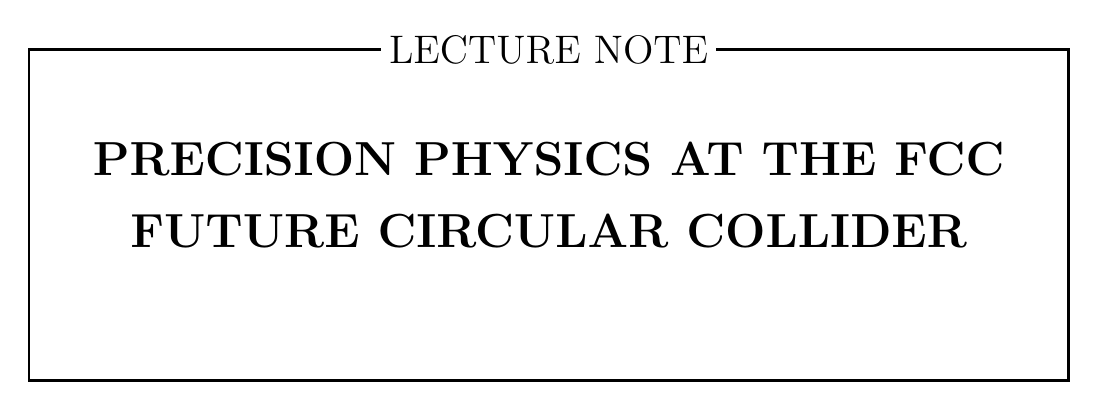
\begin{tikzpicture}
\draw[line width=0.9pt] (0,0) rectangle (13.2,4.2);
\node[fill=white,inner sep=3pt,font=\Large] at (6.6,4.2) {LECTURE NOTE};
\node[font=\bfseries\fontsize{17}{21}\selectfont,align=center] at (6.6,2.35) {PRECISION PHYSICS AT THE FCC\\[0.25em]FUTURE CIRCULAR COLLIDER};
\end{tikzpicture}

\vspace{1.3cm}
{\Large Graduate-level supporting lecture notes\par}
\vspace{0.35cm}
{\large Higgs, electroweak, top, flavour, SMEFT and BSM precision physics\par}
\vspace{1.2cm}

\begin{guidelinebox}
\vspace{0.25cm}
\itshape
These notes provide a polished teaching draft for a graduate lecture note on precision physics at the Future Circular Collider. The emphasis is on the FCC-ee precision programme as a Higgs, electroweak, top, flavour and BSM search machine, and on the way FCC-hh completes the programme at the energy frontier. The text combines formulas, process definitions, figures, guided checks, examples and exercises. Numerical projections are quoted as baseline or illustrative projections and are source-attributed to the FCC Feasibility Study, FCC CDR, ESPPU-era documents, or dedicated studies as indicated.
\end{guidelinebox}

\vfill
{\normalsize Prepared for advanced MSc/PhD teaching and FCC study preparation\par}
{\textbf{Hamzeh Khanpour}\par}
{\normalsize \texttt{hamzeh.khanpour@fis.agh.edu.pl}\par}
{\texttt{https://view.fis.agh.edu.pl/staff/hamzeh.khanpour/}\par}
{\normalsize \today\par}
\end{titlepage}

\tableofcontents
\newpage

\section*{Preface}
\addcontentsline{toc}{section}{Preface}
This lecture note is a compile-ready graduate teaching draft designed to support a course or advanced seminar on precision physics at the Future Circular Collider, using the FCC Feasibility Study Report as the main baseline and the FCC Conceptual Design Report for historical context~\cite{FCCFSRVol1,FCCFSRVol2,FCCFSRVol3,FCCCDRVol1,FCCCDRVol2,FCCCDRVol3}. It is based on the FCC Feasibility Study Report, the FCC Conceptual Design Report, the FCC integrated-programme manifesto, recent ECFA Higgs/electroweak/top factory material, top-threshold studies, SMEFT interpretation papers, and curated figures from the local \texttt{Figs/} directory.

The note is deliberately pedagogical. Each major topic is introduced through the physical process, the observable, the leading formula, the uncertainty logic and the interpretation framework. The boxes labelled Definition, Remark, Example, Guided checks and Take-home message are intended to make the material usable in lectures and self-study. The text distinguishes projections from measurements and avoids treating any future precision number as guaranteed.

\section*{Conventions and notation}
\addcontentsline{toc}{section}{Conventions and notation}
\begin{itemize}[leftmargin=1.7em]
\item Natural units are used: \(\hbar=c=1\).
\item Centre-of-mass energy is denoted by \(\sqrt{s}\).
\item Branching ratios are denoted by \(\BR\), and total widths by \(\Gamma\).
\item Higgs coupling modifiers are denoted by \(\kappa_i\).
\item SMEFT Wilson coefficients are denoted by \(C_i\), with scale \(\Lambda\) written explicitly unless stated otherwise.
\item Projected FCC-ee numbers are treated as scenario-dependent estimates, not as measured results.
\end{itemize}


\newpage
\section{Motivation and physics landscape}
\begin{guidelinebox}
This chapter explains why a new precision collider programme is scientifically motivated after the HL-LHC. The guiding idea is that heavy or weakly coupled new physics can leave small but correlated distortions in Standard Model observables, and that the FCC programme is designed to test these distortions with a combination of FCC-ee precision and FCC-hh energy reach.
\end{guidelinebox}

\subsection{Learning goals and key questions}
After this chapter, the reader should be able to explain why precision measurements are a discovery tool, why FCC-ee and FCC-hh are complementary, and why the FCC physics case cannot be reduced to a single flagship observable. The key questions are:
\begin{itemize}[leftmargin=1.6em]
\item What can be learned if no new particle has been produced directly at the LHC or HL-LHC?
\item How can a sub-percent deviation in a low-energy observable probe a multi-TeV scale?
\item Why does FCC-ee need the Z pole, WW threshold, Higgs factory and top threshold rather than only one energy point?
\item Why is FCC-hh not a separate physics programme, but the energy-frontier completion of the precision stage?
\end{itemize}

The present lecture note is built around the central FCC chain
\begin{equation}
\begin{aligned}
  &\text{large clean samples at FCC-ee}
  \longrightarrow \text{overconstrained SM precision tests} \\
  &\longrightarrow \text{indirect BSM sensitivity}
  \longrightarrow \text{direct exploration at FCC-hh} .
\end{aligned}
\end{equation}
This chain is not a slogan; it is the operational logic behind the selection of observables, detector requirements and theory calculations in the FCC Feasibility Study Report~\cite{FCCFSRVol1} and in the integrated FCC physics manifesto~\cite{FCCManifesto2025}.

\begin{definition}{Precision observable}{precision-observable}
A precision observable is a measurable quantity for which the experimental and theoretical uncertainties are small enough that loop effects, interference effects, or suppressed new-physics contributions can become visible. Examples include \(\mZ\), \(\gZ\), \(\mW\), \(\sintw\), \(\sigma_{ZH}\), Higgs branching fractions, top-threshold cross sections and rare flavour observables.
\end{definition}

\subsection{From direct discovery to precision discovery}
The traditional discovery mode of a collider is direct: if a new state has mass below the partonic centre-of-mass energy and couples sufficiently strongly, it can be produced on shell. At a hadron collider this is schematically
\begin{equation}
  pp \to X_{\rm BSM} + \cdots,
  \qquad
  X_{\rm BSM} \to \text{visible or invisible final states} .
\end{equation}
Precision discovery is different. A heavy state with mass \(M\) may be too heavy to be produced directly at FCC-ee, but it can still contribute virtually to an observable. If its low-energy effect is captured by a dimension-six operator, then a typical fractional shift has the form
\begin{equation}
  \frac{\delta \mathcal O}{\mathcal O_{\rm SM}}
  \sim C_i\frac{v^2}{\Lambda^2}
  \quad \text{or} \quad
  \frac{\delta \mathcal O}{\mathcal O_{\rm SM}}
  \sim C_i\frac{E^2}{\Lambda^2},
  \label{eq:precision-scale-intro}
\end{equation}
where \(v\simeq246\\,\GeV\) is the Higgs vacuum expectation value, \(E\) is a characteristic energy of the process, \(C_i\) is a dimensionless Wilson coefficient and \(\Lambda\) is the new-physics scale. Equation~\eqref{eq:precision-scale-intro} is the simplest reason why per-mille measurements are valuable.

\begin{examplebox}{Scale estimate from a per-mille measurement}{scale-estimate}
Suppose a Higgs or electroweak coupling is constrained at the level \(\delta\mathcal O/\mathcal O_{\rm SM}=10^{-3}\), and suppose the coefficient is \(C_i=1\). If the effect scales as \(v^2/\Lambda^2\), then \(\Lambda\sim v/\sqrt{10^{-3}}\simeq7.8\\,\TeV\). If an observable at a higher energy scales instead as \(E^2/\Lambda^2\), with \(E=365\\,\GeV\), the same per-mille precision corresponds to \(\Lambda\sim11.5\\,\TeV\). This estimate is crude because realistic fits include correlations, flavour assumptions and loop factors, but it captures the basic lever arm.
\end{examplebox}

\subsection{The FCC as an integrated programme}
FCC-ee and FCC-hh should be viewed together. FCC-ee is not simply a Higgs factory; it is a Z factory, a WW threshold machine, a Higgs factory, a top-threshold machine, and a high-statistics top/electroweak machine at 365 GeV. FCC-hh then extends the programme to direct production of new states and high-energy precision measurements. The integrated structure is particularly powerful because the two stages test the same physics in different ways. A deviation in a Higgs or electroweak coupling at FCC-ee would suggest which sectors FCC-hh should probe directly; conversely, a discovery at FCC-hh would need the FCC-ee measurements to identify its low-energy footprint.

Figure~\ref{fig:fcc-runsequence} is used here as a visual anchor for the surrounding discussion. The important point is not only the numerical projection shown in the figure, but also the way in which the relevant FCC observable is connected to a physical parameter of the Standard Model or to a possible deviation from it.
\begin{figure}[H]
  \centering
  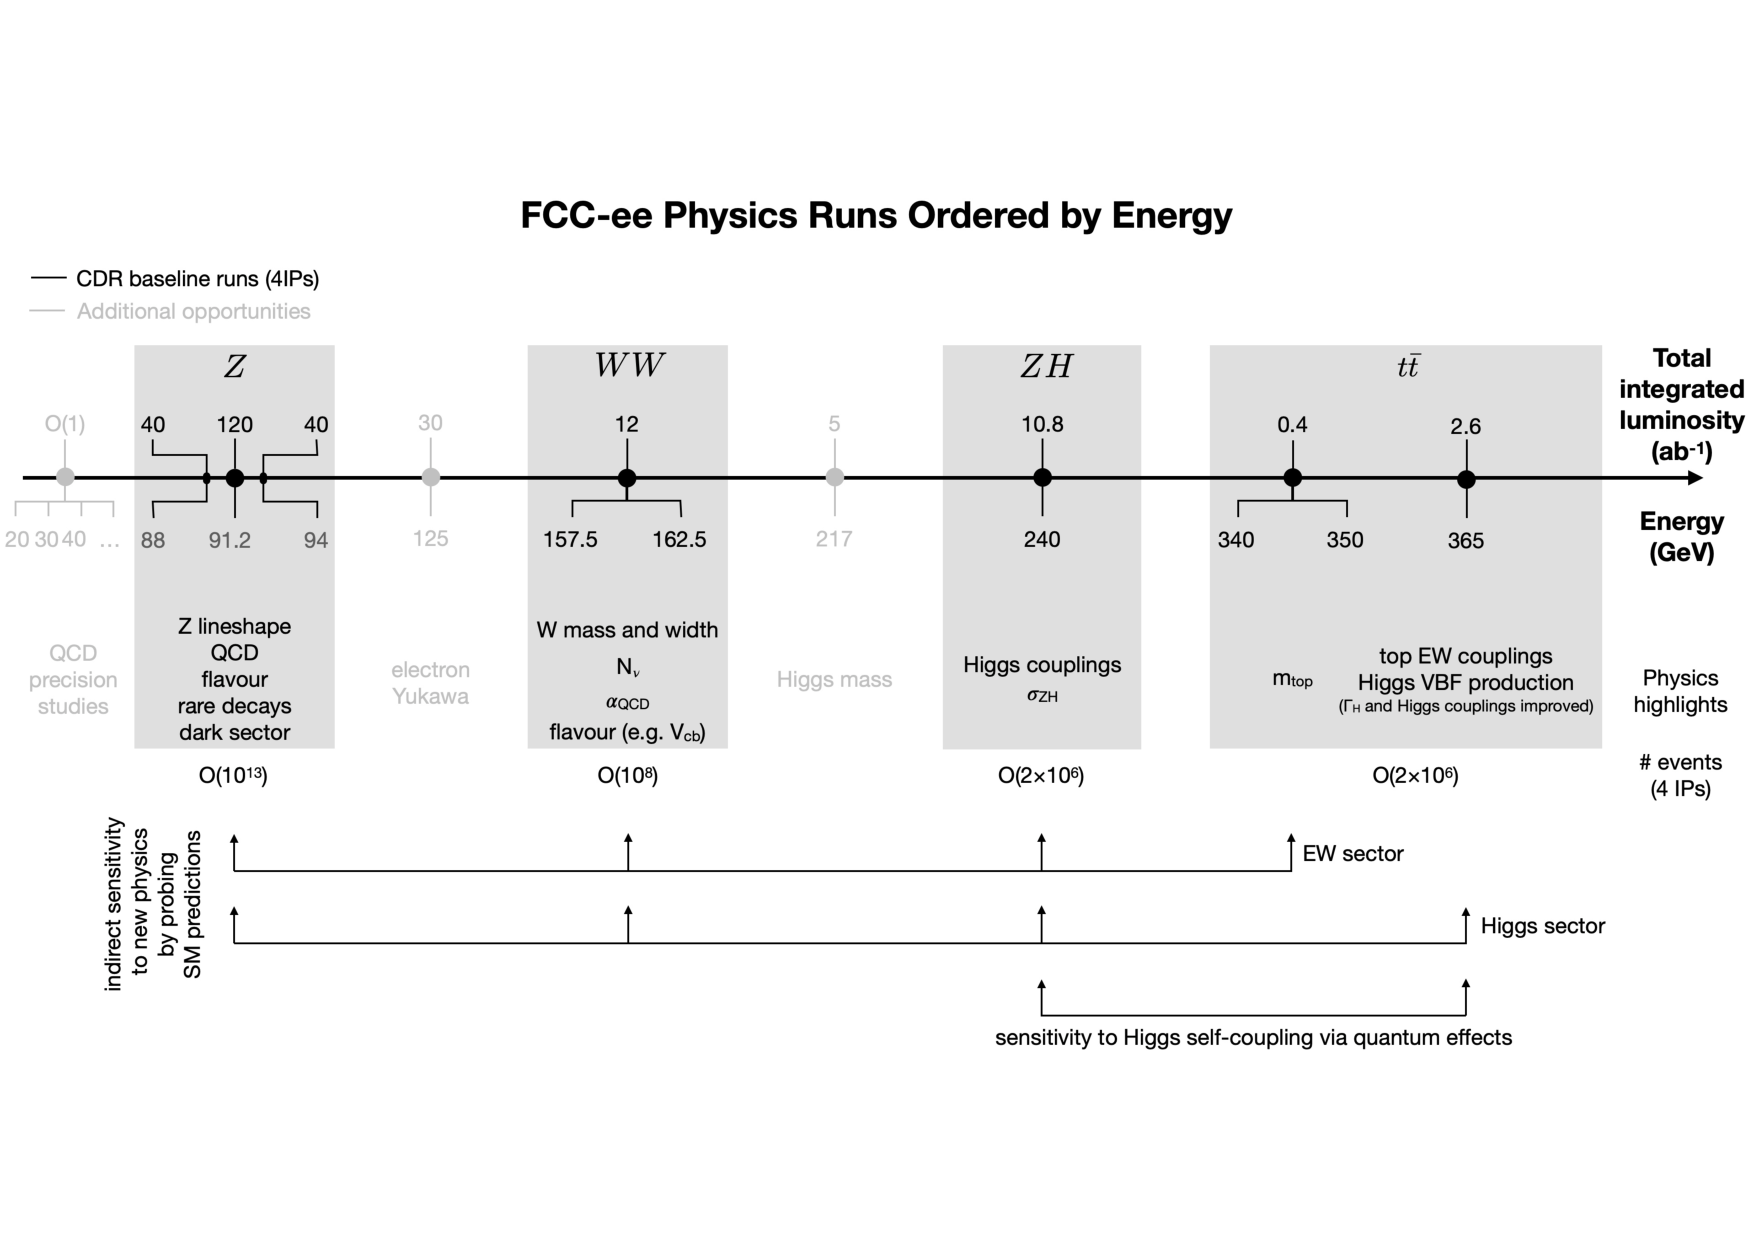
\includegraphics[width=0.95\textwidth]{Figs/FCC-ee_RunSequence_2024_09_26.pdf}
  \caption{Baseline FCC-ee running points and physics programme. The figure summarises how the Z pole, WW threshold, Higgs factory, top threshold and 365 GeV runs form a coherent precision programme. Source: Ref.~\cite{FCCManifesto2025}.}
  \label{fig:fcc-runsequence}
\end{figure}
The key lesson is that a projection is meaningful only after the measured observable, the assumptions entering its extraction, and the dominant uncertainty sources have been identified.

Figure~\ref{fig:circos-fcc-ee} is used here as a visual anchor for the surrounding discussion. The important point is not only the numerical projection shown in the figure, but also the way in which the relevant FCC observable is connected to a physical parameter of the Standard Model or to a possible deviation from it.
\begin{figure}[H]
  \centering
  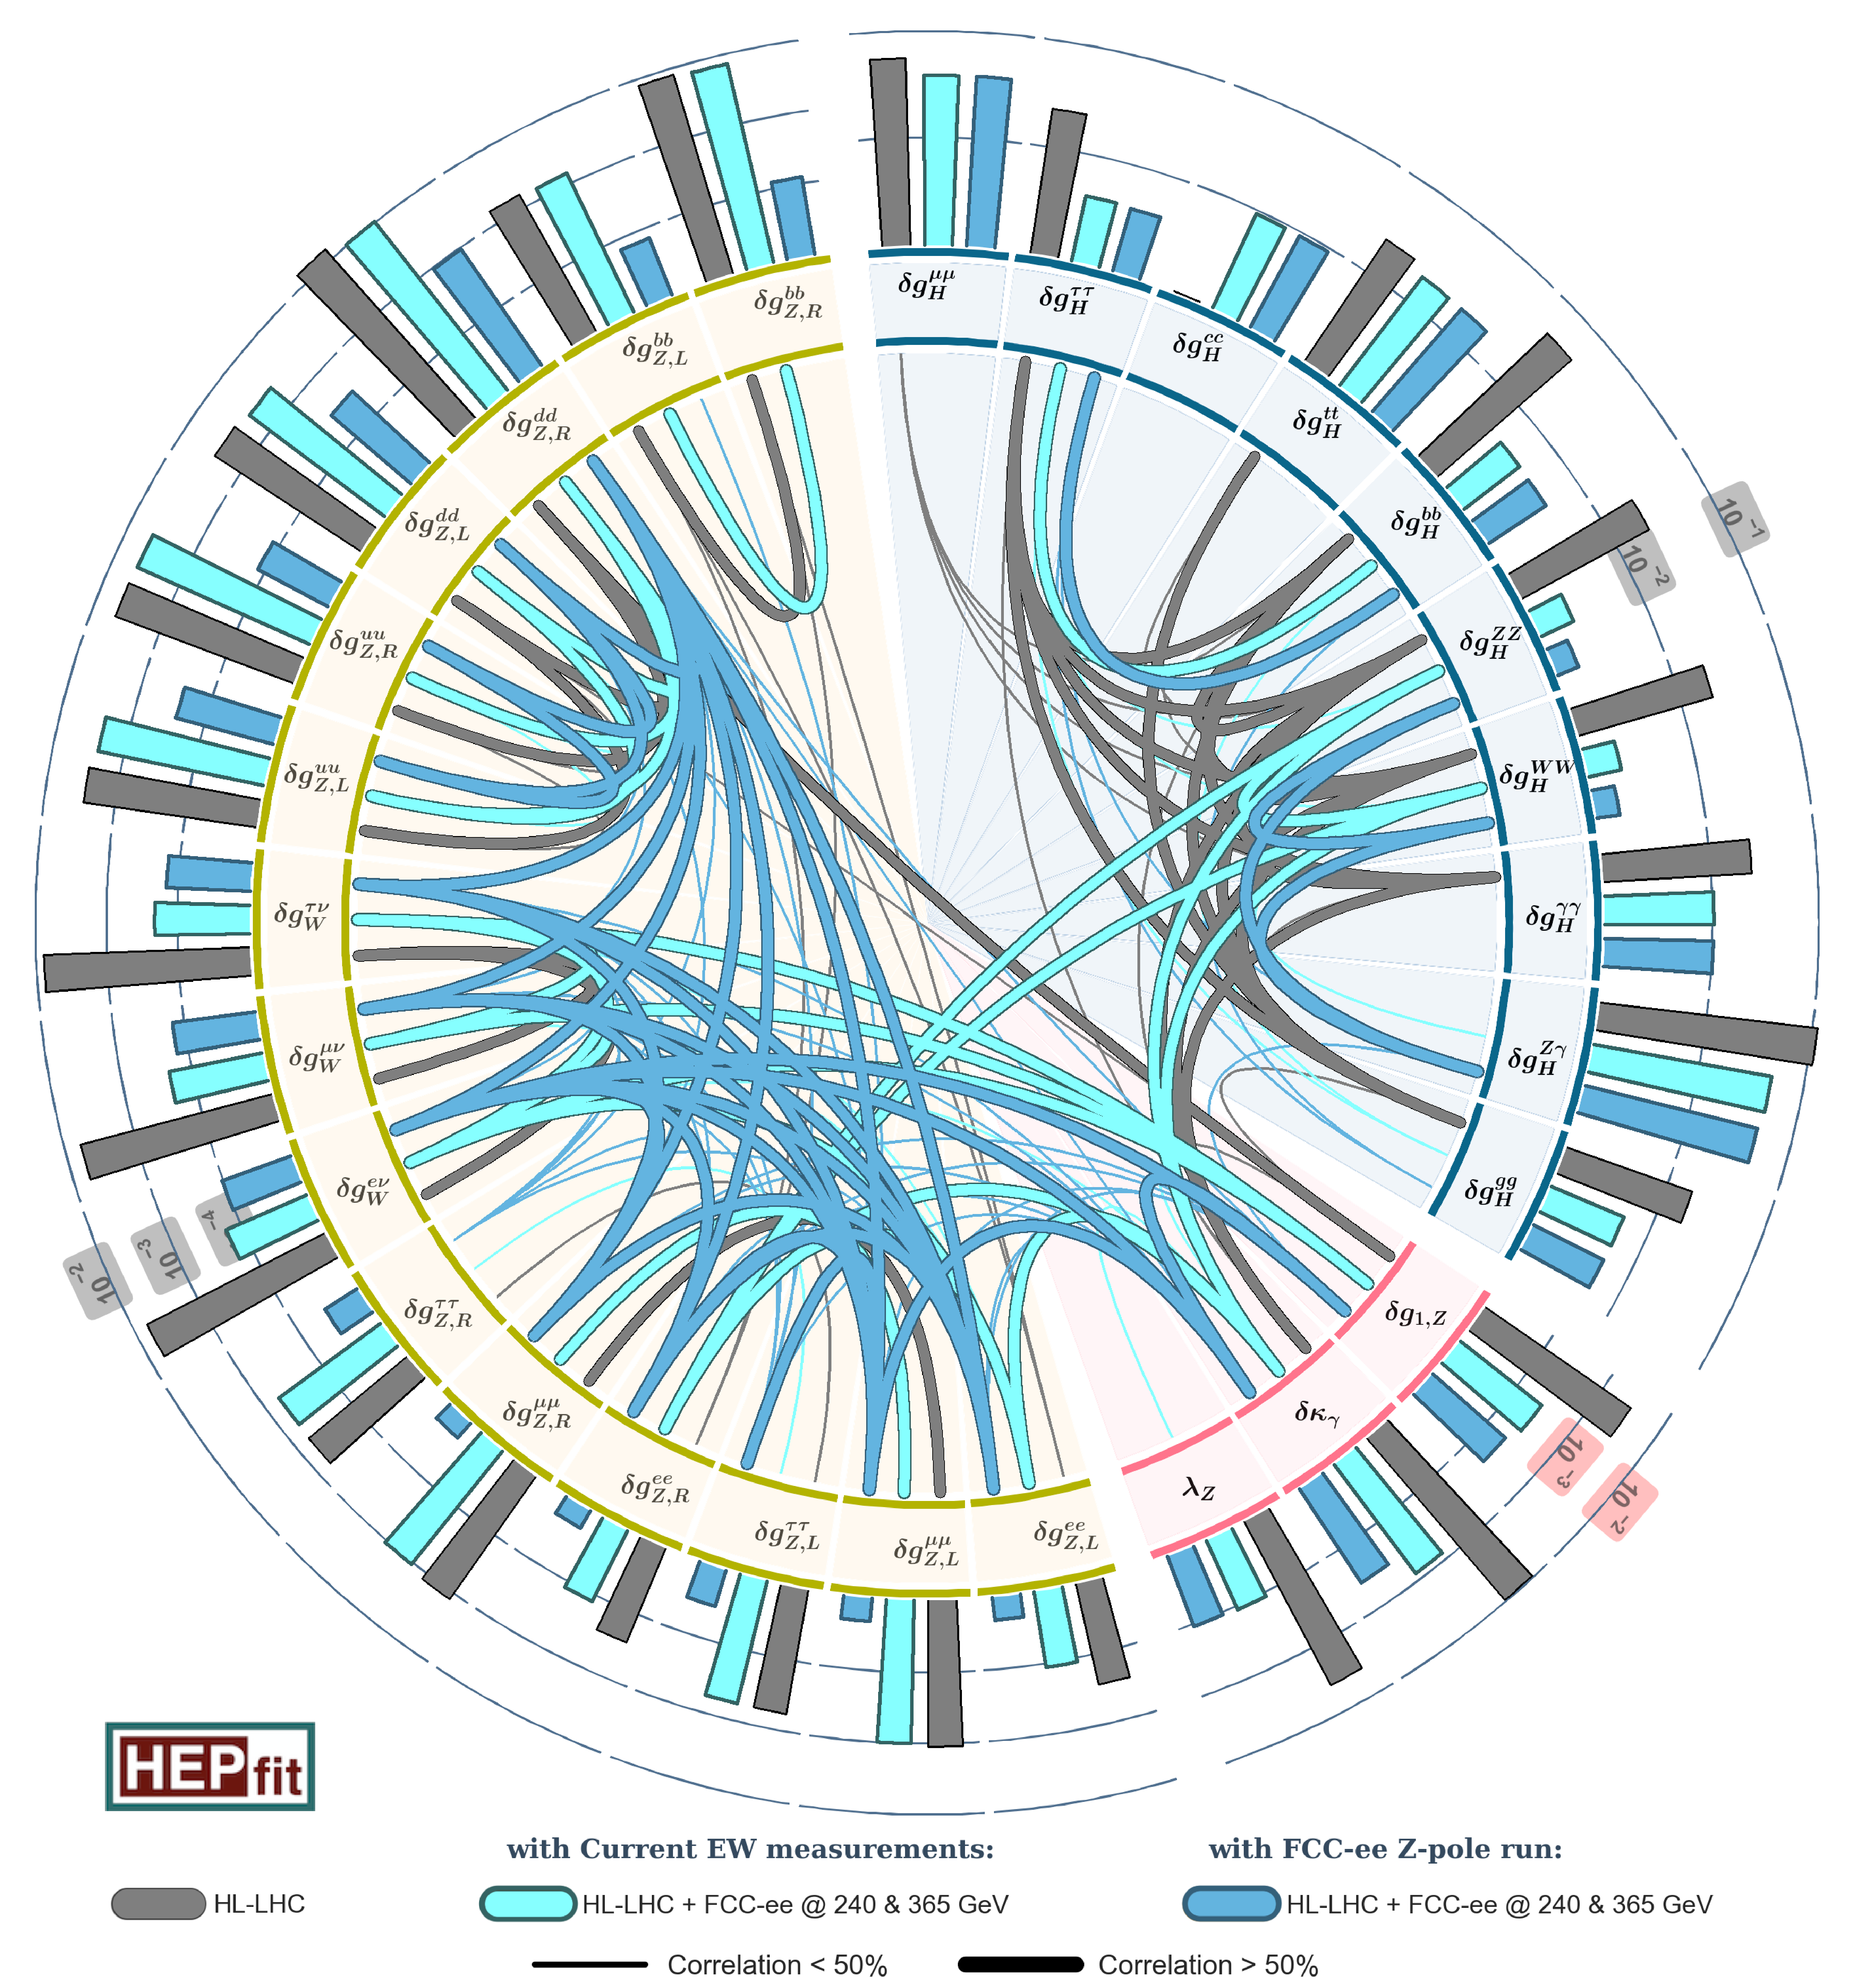
\includegraphics[width=0.92\textwidth]{Figs/circos_FCCee_nomargin_newFSR.pdf}
  \caption{Circular overview of the FCC-ee physics programme and its connections among Higgs, electroweak, top, flavour and BSM observables. Source: Ref.~\cite{FCCFSRVol1}.}
  \label{fig:circos-fcc-ee}
\end{figure}
The key lesson is that a projection is meaningful only after the measured observable, the assumptions entering its extraction, and the dominant uncertainty sources have been identified.

\begin{remarkbox}{Projection versus measurement}{projection-vs-measurement}

Throughout these notes, projected FCC precisions are not treated as measurements. They are estimates obtained under explicit assumptions about luminosity, detector performance, beam-energy calibration, flavour tagging, theoretical calculations and correlations among systematic uncertainties. When the same observable appears in both the Conceptual Design Report and the Feasibility Study Report era, the newer Feasibility Study Report or ESPPU-era numbers should be used as the default baseline, while the older CDR values remain useful for understanding the evolution of assumptions.

\end{remarkbox}

\begin{guidedchecksbox}
\begin{enumerate}[leftmargin=1.6em]
\item Use Eq.~\eqref{eq:precision-scale-intro} to estimate the scale probed by a \(0.3\%\) coupling measurement for \(C_i=1\).
\item Explain why a clean \(e^+e^-\) initial state is valuable even when the centre-of-mass energy is lower than that of a hadron collider.
\item Give one example of a direct search at FCC-hh and one indirect precision test at FCC-ee that could probe related new physics.
\end{enumerate}
\end{guidedchecksbox}

\subsection{A map of the lecture note}
The note proceeds from machine concept to physics interpretation. Chapter~2 describes the run plan. Chapter~3 introduces precision as an indirect discovery tool and sets up the EFT language. Chapters~4--6 treat the core FCC-ee precision pillars: Higgs, electroweak and top physics. Chapter~7 explains how these measurements are combined in global interpretations. Chapters~8 and 9 broaden the programme to flavour, tau and BSM searches. Chapters~10 and 11 discuss the theory and detector requirements that make the precision claims credible. Chapter~12 explains the FCC-hh stage, and Chapter~13 gives a synthesis.

\subsection{Exercises}
\begin{enumerate}[leftmargin=1.6em]
\item Derive the scaling \(\Lambda\sim v/\sqrt{\delta}\) for an observable whose fractional deviation is \(\delta=Cv^2/\Lambda^2\).
\item Explain why precision measurements can probe new physics even if the collider energy is below the mass of the new particle.
\item Write a one-paragraph comparison of FCC-ee and FCC-hh in terms of initial state, dominant strengths and physics role.
\end{enumerate}

\begin{takehomebox}
The FCC precision programme is a redundancy programme: the same underlying physics is tested through Higgs rates, electroweak pseudo-observables, top-threshold observables, flavour transitions, rare decays and high-energy tails. The power is in the correlations.
\end{takehomebox}


\newpage
\section{FCC machine concept and run plan}
\begin{guidelinebox}
This chapter translates the FCC-ee run plan into a physics map. Each energy point is chosen because a particular Standard Model process becomes exceptionally clean or exceptionally abundant there. The FCC-ee design therefore functions as a sequence of specialised precision machines within a single collider programme.
\end{guidelinebox}

\subsection{Learning goals and run-plan logic}
The main goal is to understand why the FCC-ee baseline contains several energy points. A single energy would not provide the needed combination of Higgs, electroweak, top, flavour and BSM observables. The rough sequence is
\begin{equation}
  \begin{array}{rclcl}
  \sqrt{s}\simeq 88,91,94\,\GeV &:& e^+e^-\to Z &\Rightarrow& \text{Tera-Z electroweak, flavour, tau, BSM},\\[0.2em]
  \sqrt{s}\simeq 157,163\,\GeV &:& e^+e^-\to W^+W^- &\Rightarrow& \mW,\ \gW,\ \text{diboson couplings},\\[0.2em]
  \sqrt{s}=240\,\GeV &:& e^+e^-\to ZH &\Rightarrow& \text{Higgs recoil and couplings},\\[0.2em]
  \sqrt{s}\simeq340\text{--}350\,\GeV &:& e^+e^-\to t\bar t &\Rightarrow& \mt,\ \Gt,\ \als,\ y_t,\\[0.2em]
  \sqrt{s}=365\,\GeV &:& e^+e^-\to t\bar t,\nu\bar\nu H &\Rightarrow& \text{top EW couplings and WW fusion}.
  \end{array}
\end{equation}
The values above are nominal working points. The detailed run plan can evolve, and extensions such as Higgs-pole running or additional QCD points are under study. The important conceptual point is that the programme uses energy as a diagnostic knob.

Figure~\ref{fig:fcc-runs} is used here as a visual anchor for the surrounding discussion. The important point is not only the numerical projection shown in the figure, but also the way in which the relevant FCC observable is connected to a physical parameter of the Standard Model or to a possible deviation from it.
\begin{figure}[H]
  \centering
  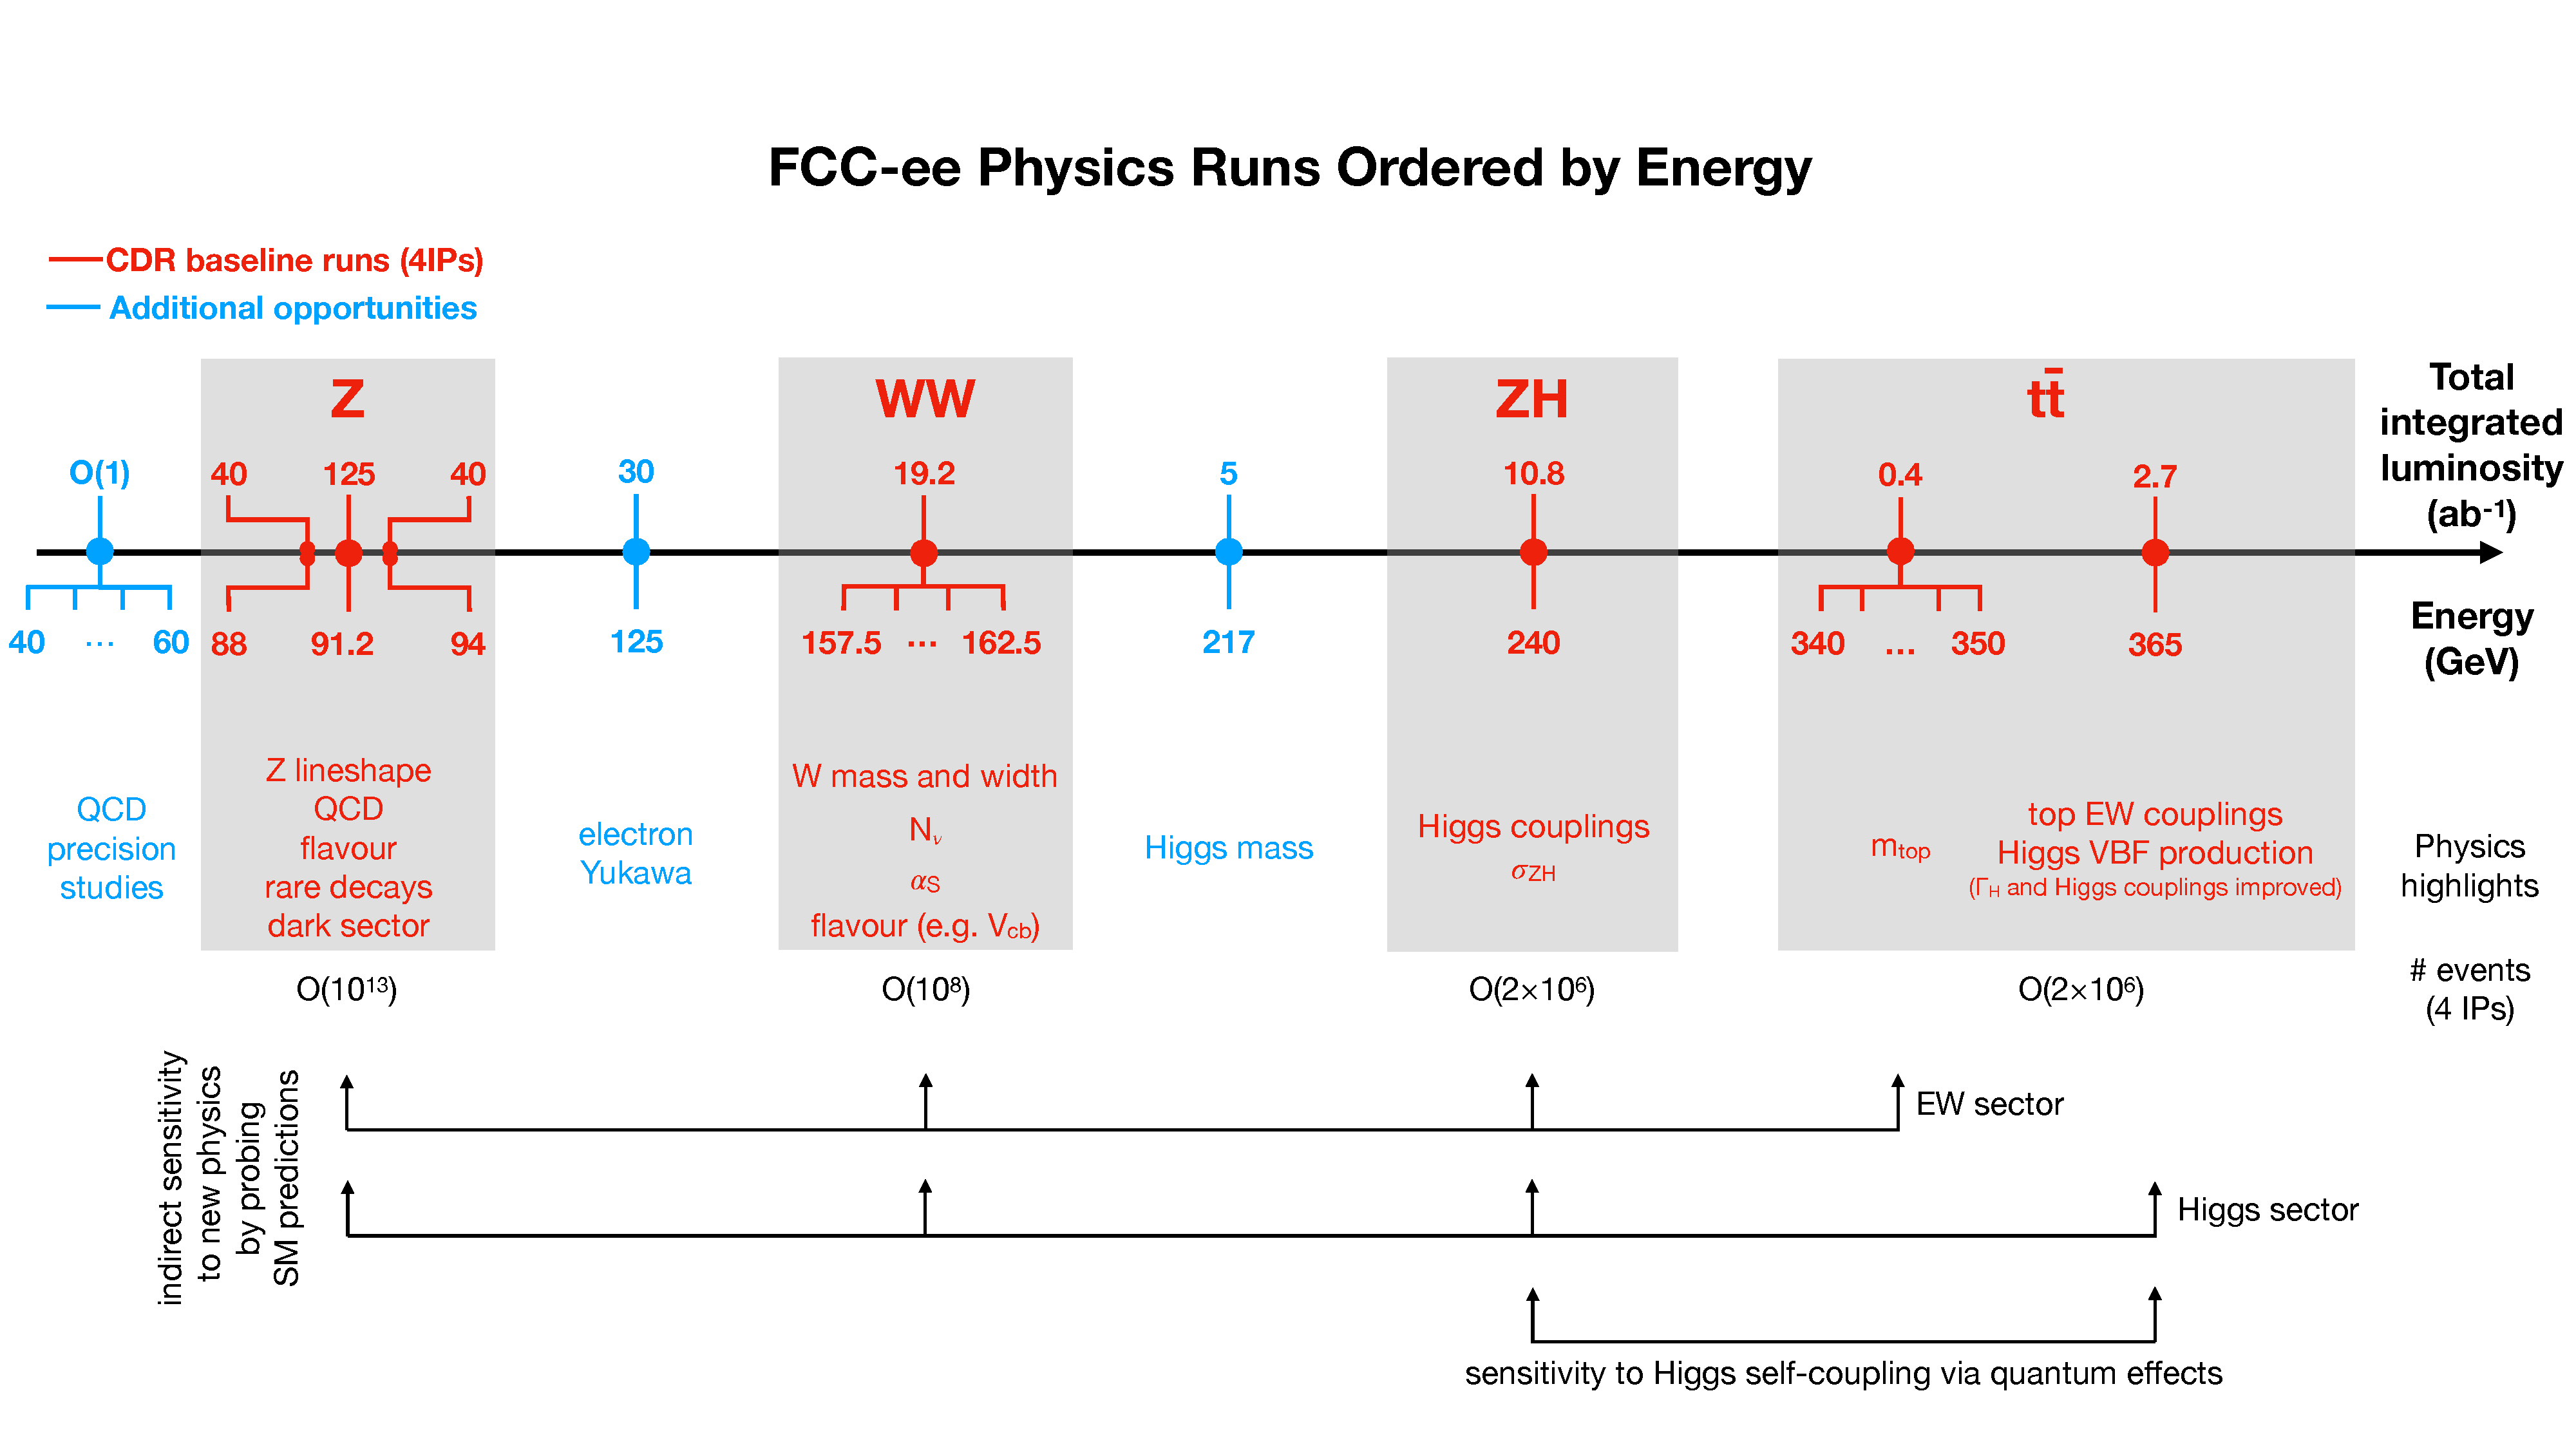
\includegraphics[width=0.95\textwidth]{Figs/FCC-runs.pdf}
  \caption{Potential FCC-ee physics programme ordered by centre-of-mass energy, showing the baseline samples and additional running possibilities. Source: Ref.~\cite{FCCFSRVol1}.}
  \label{fig:fcc-runs}
\end{figure}
The key lesson is that a projection is meaningful only after the measured observable, the assumptions entering its extraction, and the dominant uncertainty sources have been identified.

Figure~\ref{fig:fccee-lumis} is used here as a visual anchor for the surrounding discussion. The important point is not only the numerical projection shown in the figure, but also the way in which the relevant FCC observable is connected to a physical parameter of the Standard Model or to a possible deviation from it.
\begin{figure}[H]
  \centering
  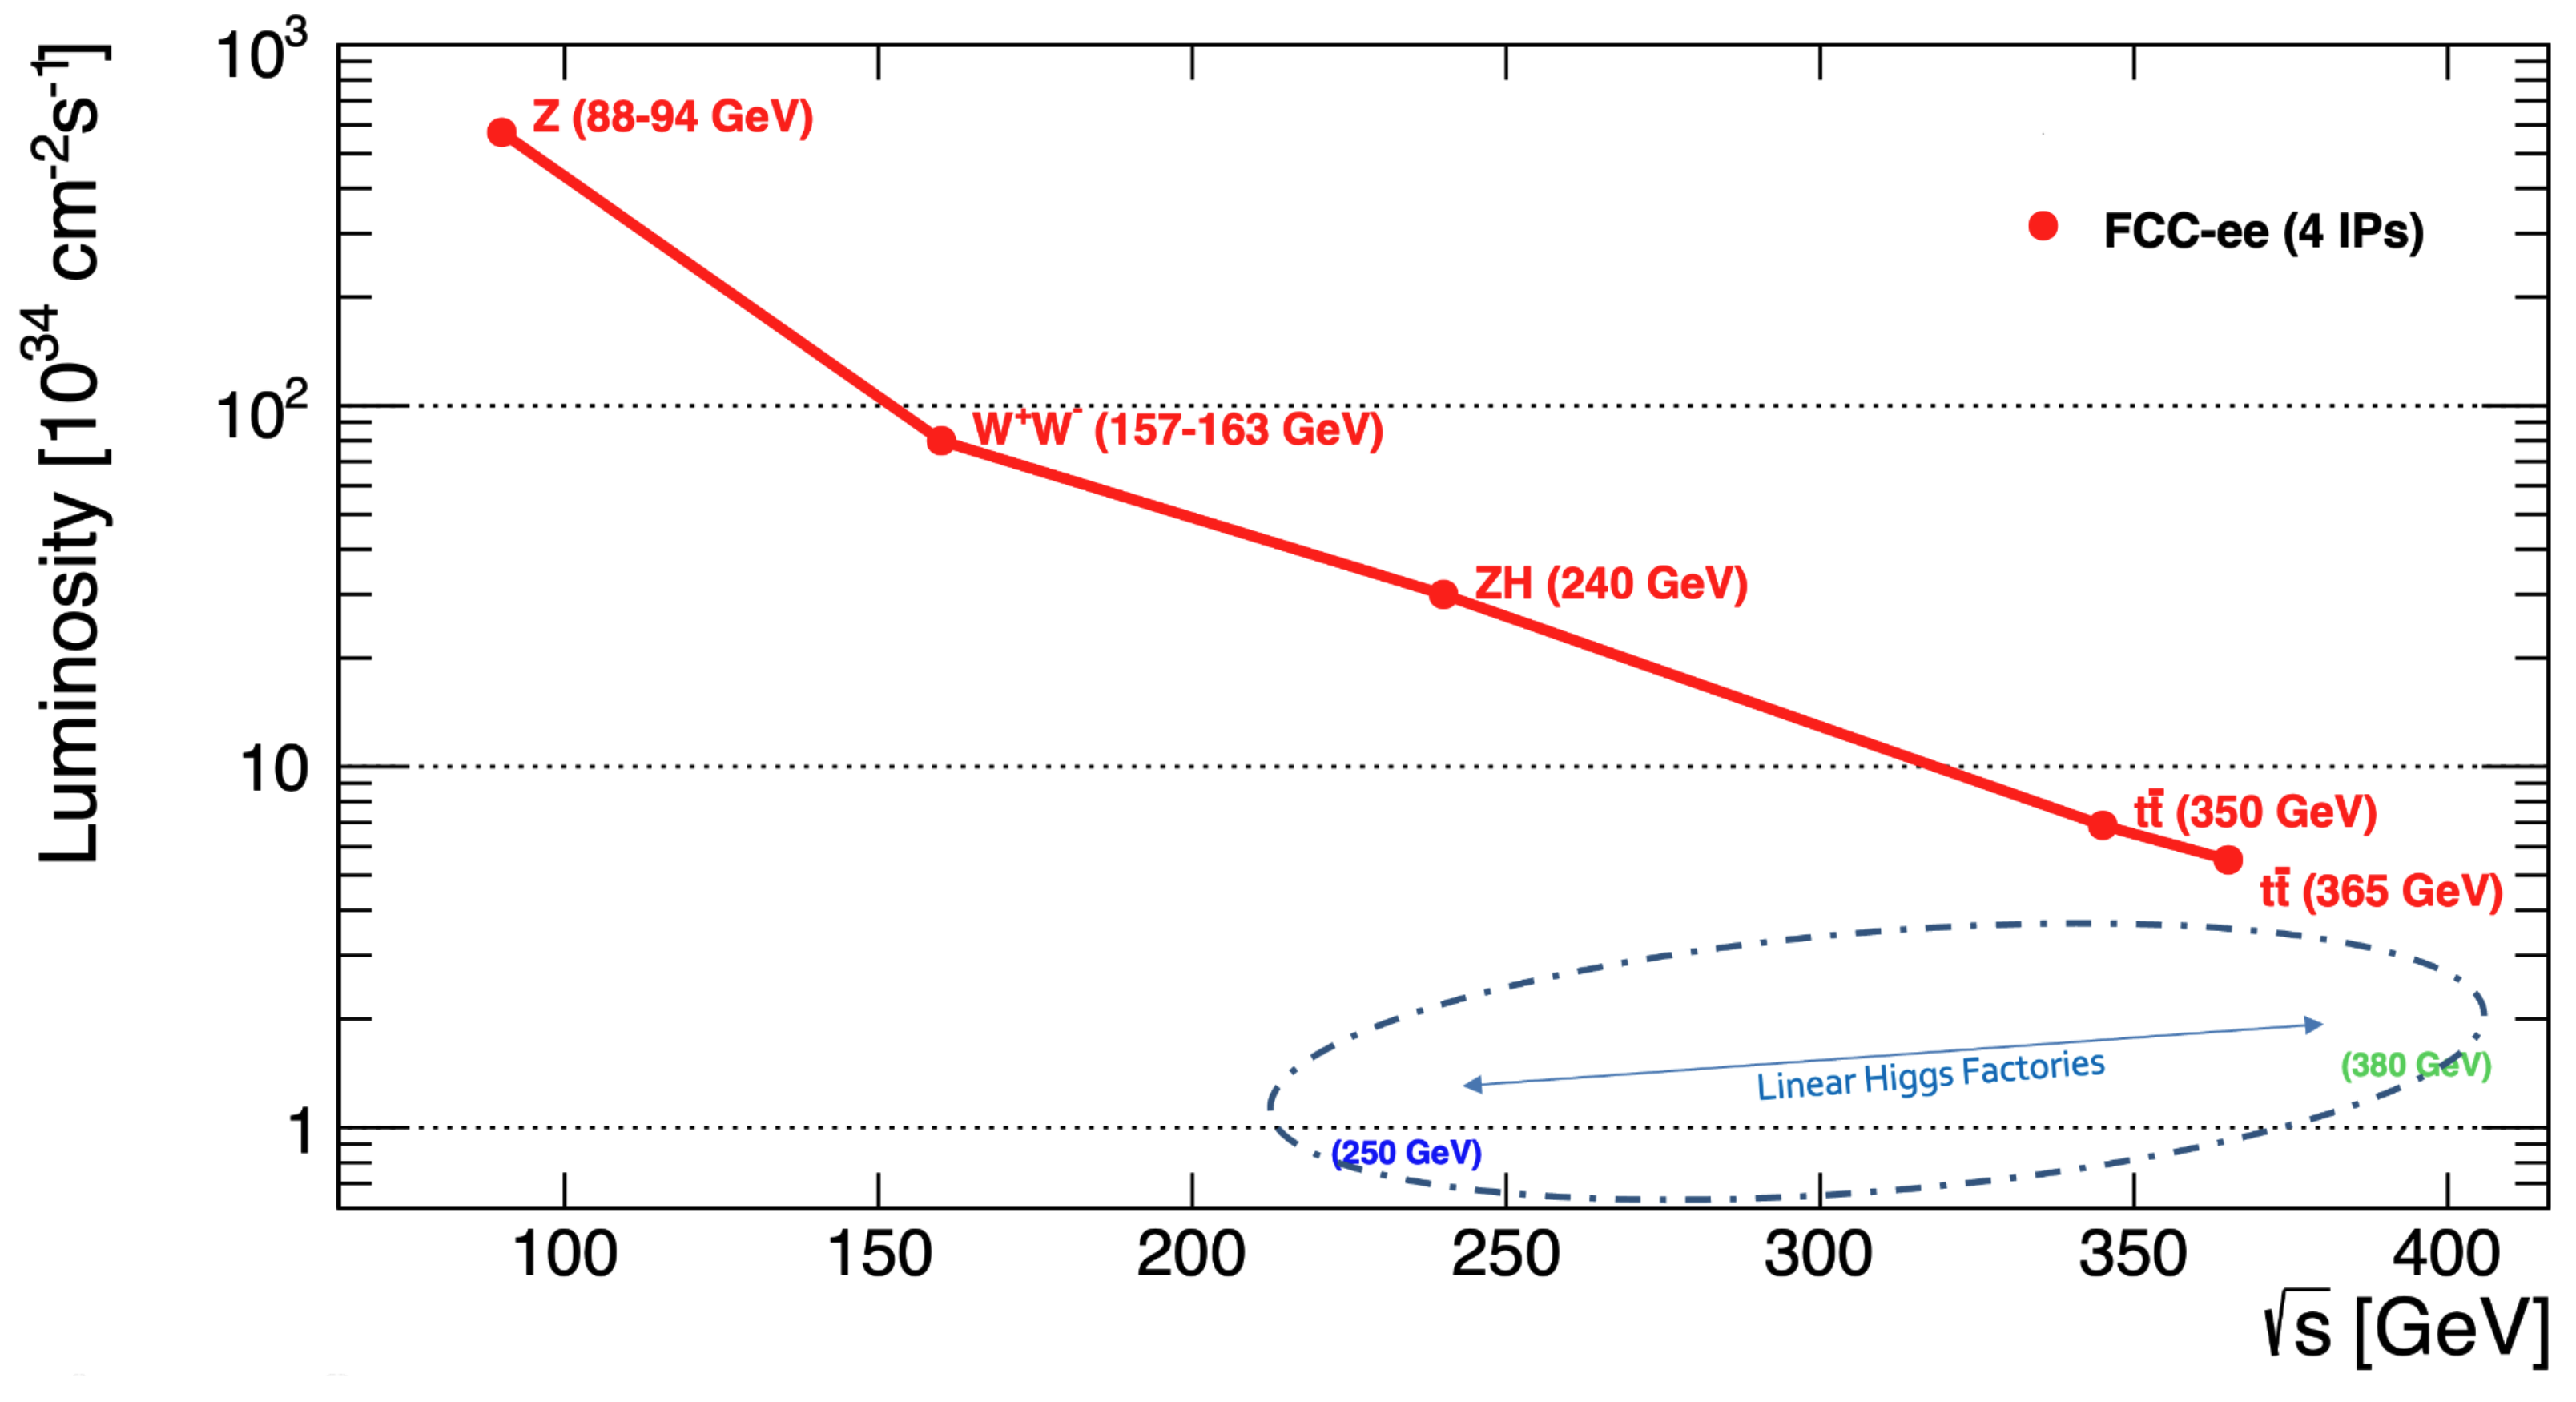
\includegraphics[width=0.95\textwidth]{Figs/FCCeeLumis2024.png}
  \caption{FCC-ee design luminosity as a function of centre-of-mass energy. The high luminosity at the Z pole and the sustained luminosity up to the top region are central ingredients of the precision programme. Source: Ref.~\cite{FCCFSRVol1}.}
  \label{fig:fccee-lumis}
\end{figure}
The key lesson is that a projection is meaningful only after the measured observable, the assumptions entering its extraction, and the dominant uncertainty sources have been identified.

Figure~\ref{fig:fcc-tunnel} is used here as a visual anchor for the surrounding discussion. The important point is not only the numerical projection shown in the figure, but also the way in which the relevant FCC observable is connected to a physical parameter of the Standard Model or to a possible deviation from it.
\begin{figure}[H]
  \centering
  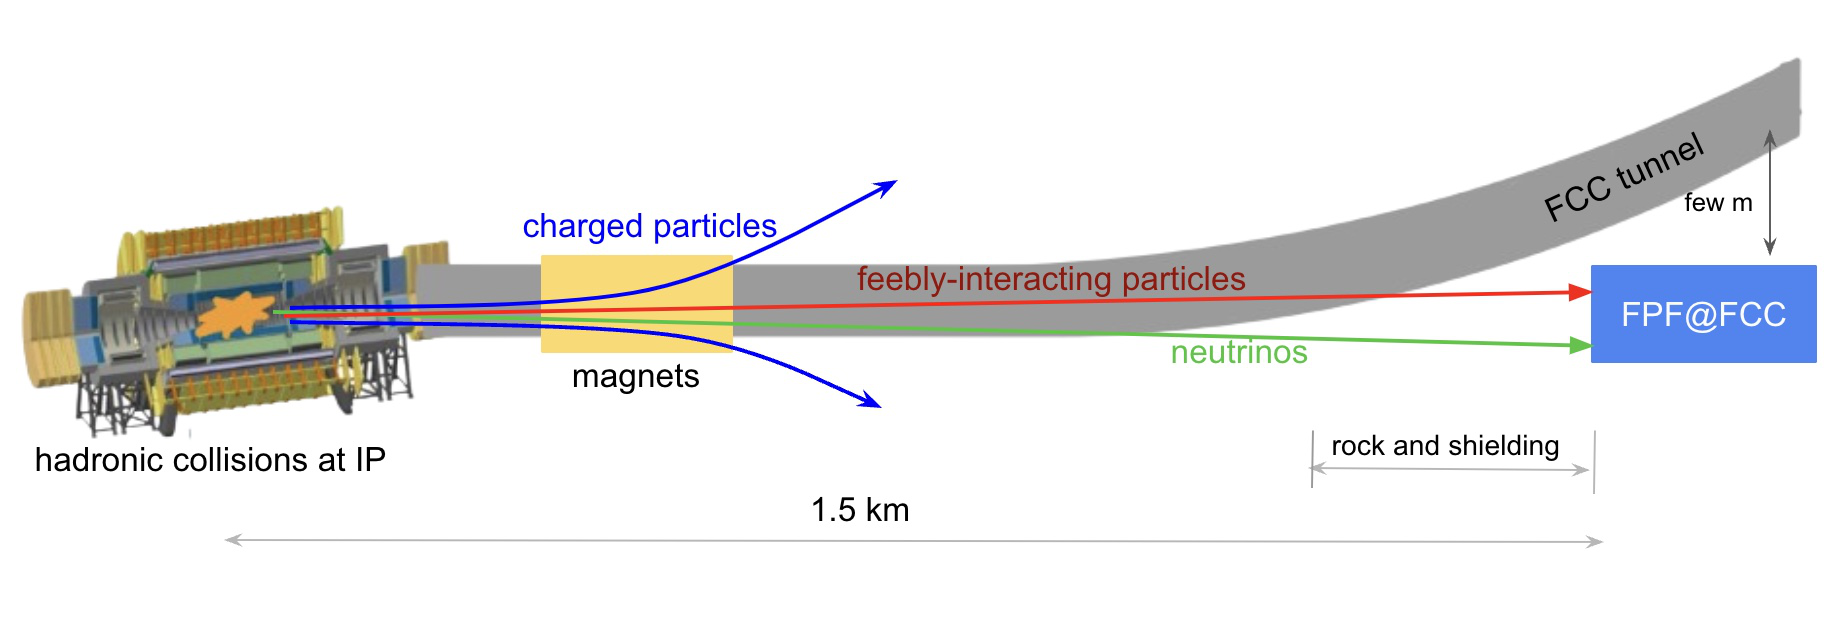
\includegraphics[width=0.80\textwidth]{Figs/FCCtunnel.png}
  \caption{Illustration of the FCC tunnel and integrated infrastructure concept. Source: Ref.~\cite{FCCFSRVol1}.}
  \label{fig:fcc-tunnel}
\end{figure}
The key lesson is that a projection is meaningful only after the measured observable, the assumptions entering its extraction, and the dominant uncertainty sources have been identified.

\begin{definition}{Working point}{working-point}
A working point is a centre-of-mass energy and luminosity configuration chosen to optimise a specific physics objective. At FCC-ee, the working points are not arbitrary: each corresponds to a threshold, resonance, or production maximum that makes a class of observables especially sensitive.
\end{definition}

\subsection{Baseline working points and target samples}
The expected event samples are enormous compared with previous lepton-collider data sets. A schematic summary is given in Table~\ref{tab:run-plan}. The numbers should be read as baseline projections rather than immutable design guarantees.
\begin{table}[H]
\centering
\small
\caption{Baseline FCC-ee working points in the four-interaction-point operation model. The luminosities and event yields are rounded projections from the FCC Feasibility Study Report Vol.~1 and the integrated-programme summary; they should be read as baseline assumptions, not as delivered measurements.}
\label{tab:run-plan}
\begin{tabularx}{\textwidth}{@{}p{2.35cm}p{2.0cm}p{2.35cm}p{2.15cm}X@{}}
\toprule
Working point & Approx. energy & Integrated luminosity & Target sample & Main physics role \\
\midrule
Z pole & 88, 91, 94 GeV & \(205\,\ab^{-1}\) & \(6\times10^{12}\,Z\) & Z lineshape, \(\mZ\), \(\gZ\), asymmetries, \(R_b\), \(R_c\), flavour, tau, rare Z decays and HNL searches.\\
WW threshold & 157, 163 GeV & \(19.2\,\ab^{-1}\) & \(2.4\times10^8\,WW\) & \(\mW\), \(\gW\), W branching fractions and diboson tests.\\
Higgs factory & 240 GeV & \(10.8\,\ab^{-1}\) & \(2.2\times10^6\,ZH\) & Inclusive \(\sigma_{ZH}\), Higgs recoil, absolute couplings and invisible/exotic decays.\\
Top threshold & 340--350 GeV & \(0.42\,\ab^{-1}\) & threshold scan & \(\mt^{\rm PS}\), \(\Gt\), \(\als\), threshold-shape tests and top-Yukawa sensitivity.\\
High energy & 365 GeV & \(2.70\,\ab^{-1}\) & \(2\times10^6\,t\bar t\) plus \(\sim370\)k extra \(ZH\) & Top electroweak couplings, WW fusion and improved Higgs width/couplings.\\
\bottomrule
\end{tabularx}
\end{table}

\begin{remarkbox}{FSR baseline versus older CDR scenarios}{fsr-cdr-baseline}
When a numerical projection has changed between the 2019 Conceptual Design Report and the 2025 Feasibility Study Report, these notes use the FSR/ESPPU-era value as the default. Older CDR values are still useful for historical comparison and for topics not yet updated, but they should not be mixed with the FSR baseline without stating the assumptions.
\end{remarkbox}

\subsection{Four interaction points and redundancy}
The move to four interaction points is not only a luminosity gain. It is also a systematic-control strategy. Four detectors provide redundancy against detector-specific biases, allow different detector technologies to be optimised for different parts of the programme, and create cross-checks that are especially valuable when the statistical uncertainties are far smaller than the systematic uncertainties.

\begin{remarkbox}{Why four experiments matter}{four-ips}
At LEP, comparisons among experiments were essential for identifying detector and beam-related effects. FCC-ee aims at much smaller uncertainties, so redundancy is not a luxury; it is a precision requirement.
\end{remarkbox}

\subsection{Collider process map}
The following process map is useful throughout the note:
\begin{align}
  e^+e^- &\to Z \to f\bar f, && \text{Z-pole electroweak and flavour physics},\\
  e^+e^- &\to W^+W^- \to 4f, && \text{W mass, width and diboson couplings},\\
  e^+e^- &\to ZH, && \text{Higgs recoil and absolute \(HZZ\) coupling},\\
  e^+e^- &\to \nu\bar\nu H, && \text{WW fusion and \(HWW\) coupling},\\
  e^+e^- &\to W^+bW^-\bar b, && \text{top-threshold physics},\\
  pp &\to X, && \text{FCC-hh direct searches and high-energy precision}.
\end{align}
Each line becomes a chapter-level theme later in the note.

\begin{guidedchecksbox}
\begin{enumerate}[leftmargin=1.6em]
\item Identify which FCC-ee working point is most directly connected to \(\sigma_{ZH}\).
\item Explain why a Z-pole run helps Higgs coupling fits, even though it does not produce Higgs bosons directly.
\item Why is the 365 GeV run useful after the 240 GeV Higgs run?
\end{enumerate}
\end{guidedchecksbox}

\subsection{Exercises}
\begin{enumerate}[leftmargin=1.6em]
\item Using the process map, write down one observable from each FCC-ee energy point and identify its dominant physics interpretation.
\item Explain why event yield alone is not enough: give one example where beam-energy calibration or theory uncertainty is expected to limit the measurement.
\item Create a short table comparing the FCC-ee and FCC-hh initial states, centre-of-mass energies, strengths and limitations.
\end{enumerate}


\newpage
\section{Precision as an indirect discovery tool}
\begin{guidelinebox}
This chapter introduces the effective-field-theory language used to connect precision observables to heavy new physics. The goal is not to develop the full SMEFT formalism, but to make clear why FCC-ee measurements must be interpreted globally rather than one observable at a time.
\end{guidelinebox}

\subsection{The EFT expansion}
If new particles are heavier than the experimental energy scale and are not produced on shell, their leading effects can be organised through higher-dimensional operators,
\begin{equation}
  \Lag_{\SMEFT}=\Lag_{\SM}+\sum_i \frac{C_i^{(6)}}{\Lambda^2}O_i^{(6)}
  +\sum_j\frac{C_j^{(8)}}{\Lambda^4}O_j^{(8)}+\cdots .
  \label{eq:smeft-lagrangian-basic}
\end{equation}
The fields and symmetries are those of the Standard Model, but the interactions are extended by all allowed gauge-invariant operators. The SMEFT is therefore not a model of one specific new particle; it is a bookkeeping framework for the low-energy footprints of many possible ultraviolet completions.

\begin{definition}{Wilson coefficient}{wilson-coeff}
The Wilson coefficient \(C_i\) measures the strength of the operator \(O_i\) after the heavy degrees of freedom have been integrated out. A coefficient can be generated at tree level, at loop level, through renormalisation-group evolution, or through matching at the heavy scale. Its interpretation depends on the assumed normalisation of \(\Lambda\).
\end{definition}

For a cross section or decay width, the expansion typically takes the schematic form
\begin{equation}
  \sigma = \sigma_{\SM}
  +\sum_i \frac{C_i}{\Lambda^2}\sigma_i^{\rm int}
  +\sum_{ij}\frac{C_iC_j}{\Lambda^4}\sigma_{ij}^{\rm quad}
  +\sum_k\frac{C_k^{(8)}}{\Lambda^4}\sigma_k^{(8)}+\cdots .
  \label{eq:sigma-expansion}
\end{equation}
The interference term is often the first term retained in a linear SMEFT analysis. The quadratic dimension-six term and dimension-eight terms enter at the same formal order in \(1/\Lambda\), but their phenomenological importance can differ depending on the observable and the model assumptions.

\begin{remarkbox}{EFT validity is an assumption, not a theorem}{eft-validity}
A SMEFT interpretation is meaningful only when the energy scale probed by the measurement is sufficiently below the scale of the new dynamics and when the truncated expansion is under control. In high-energy tails this must be checked carefully; at FCC-ee, the clean environment helps, but the issue does not disappear.
\end{remarkbox}

Figure~\ref{fig:smeft-coefficients} is used here as a visual anchor for the surrounding discussion. The important point is not only the numerical projection shown in the figure, but also the way in which the relevant FCC observable is connected to a physical parameter of the Standard Model or to a possible deviation from it.
\begin{figure}[H]
  \centering
  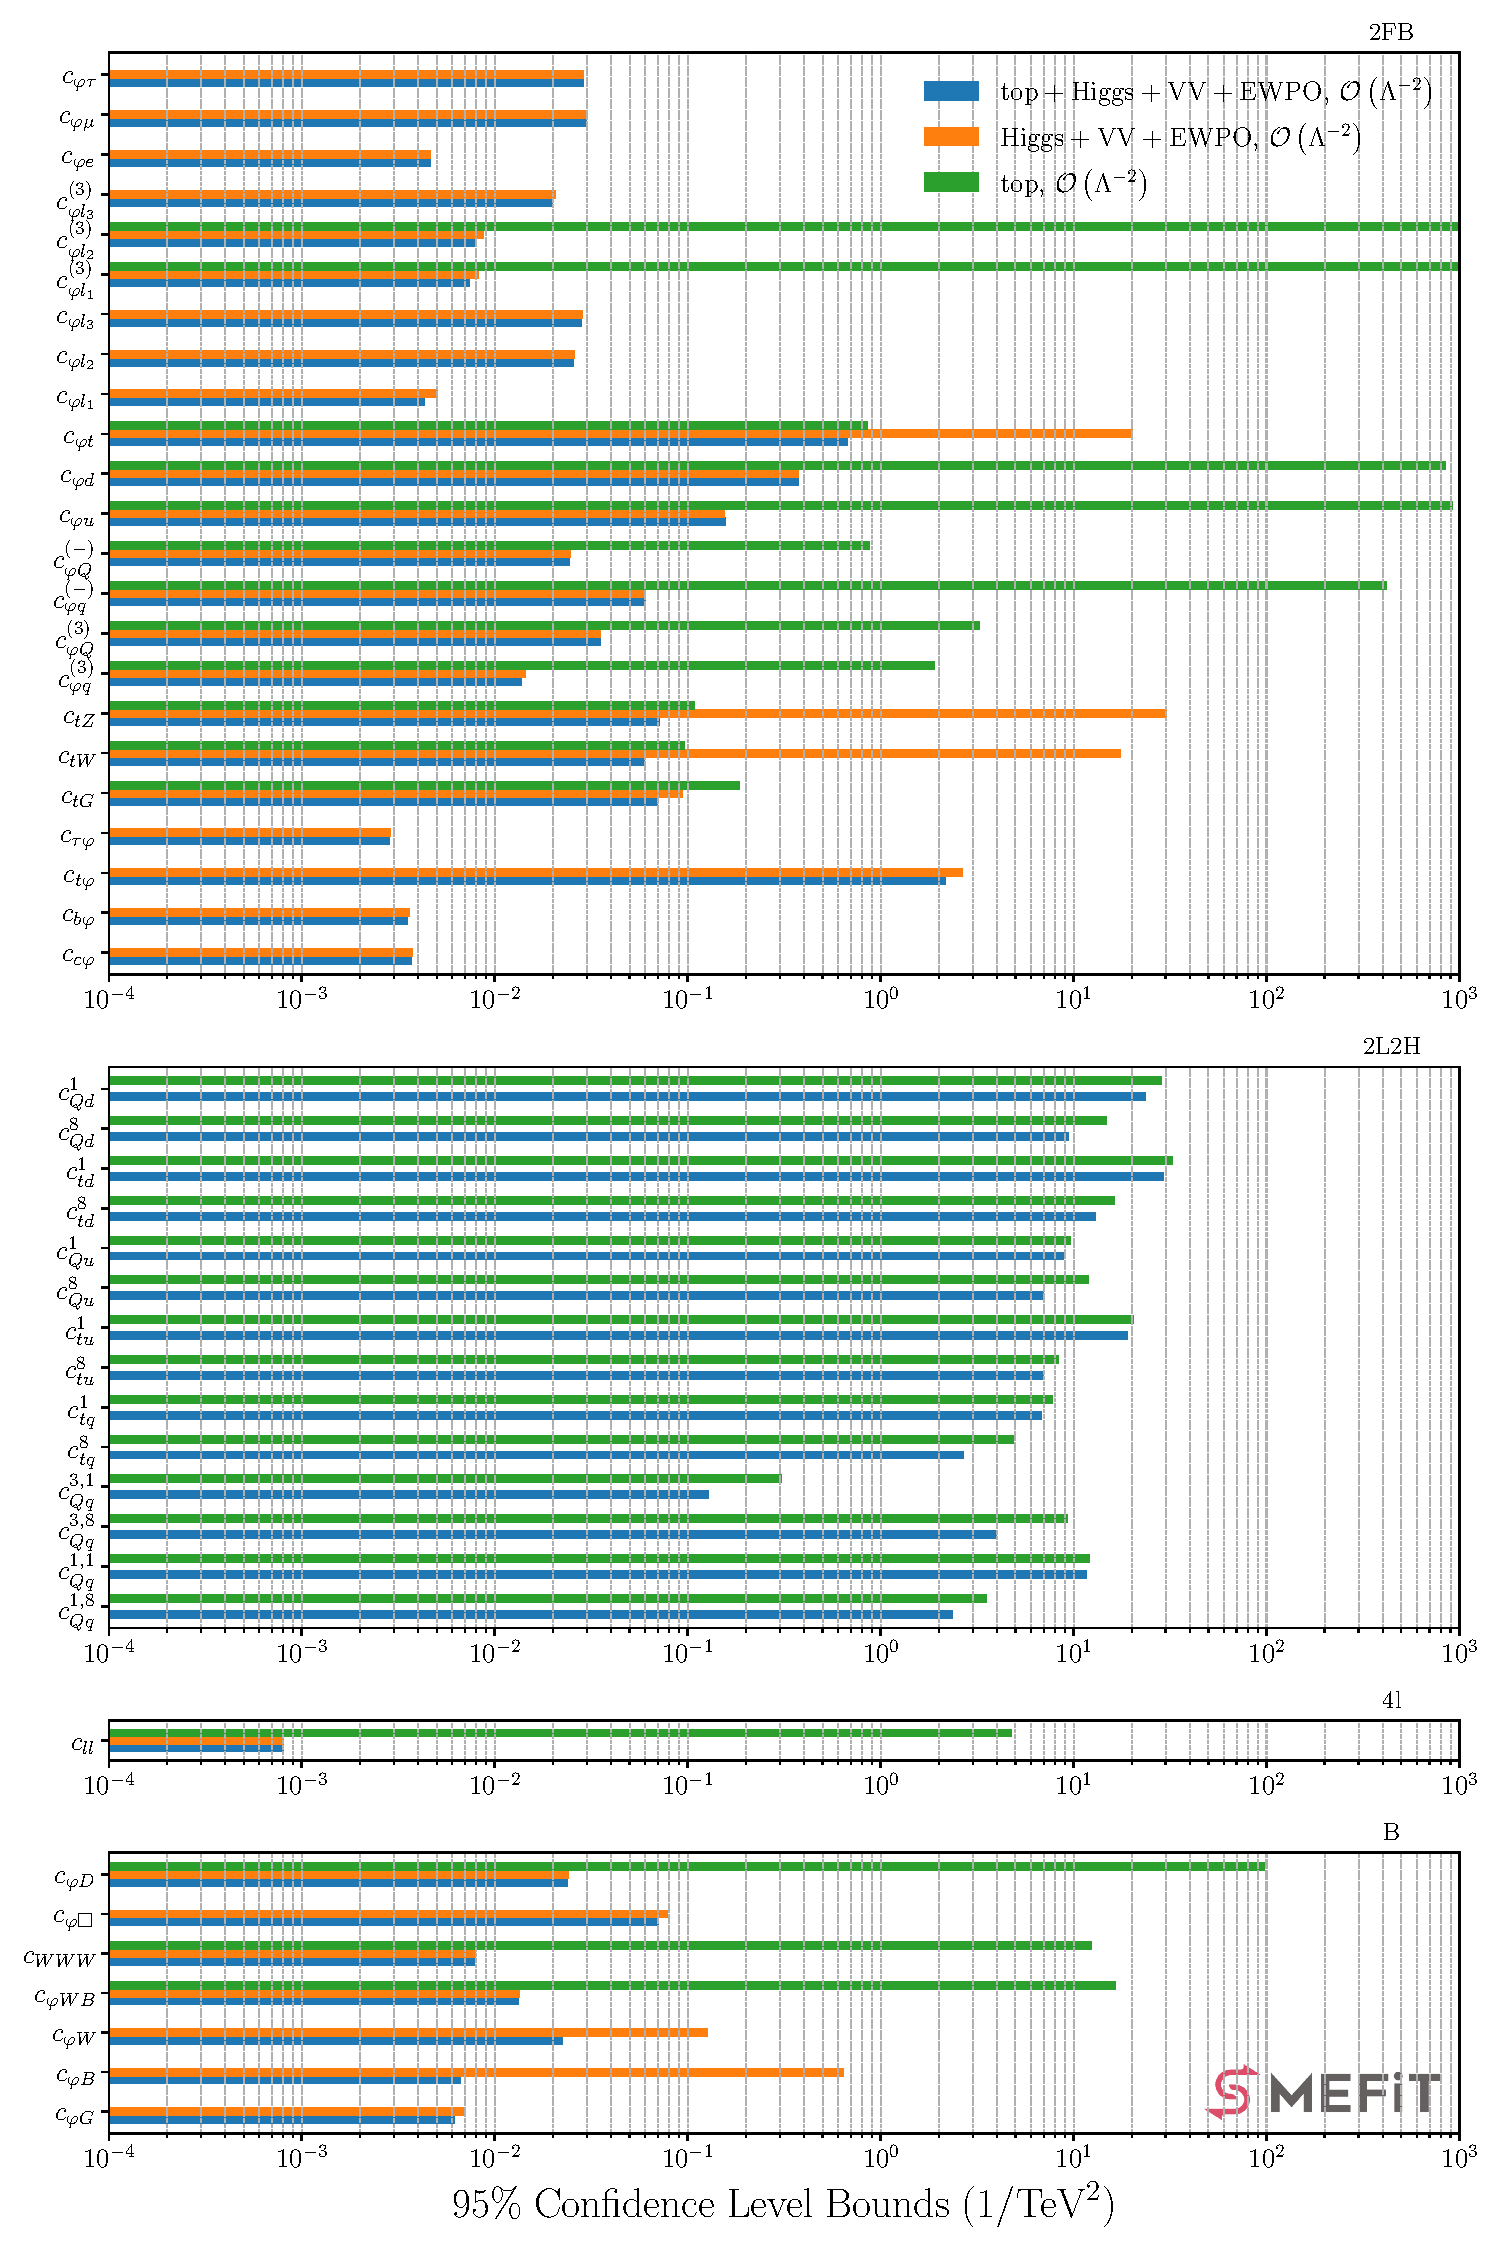
\includegraphics[width=0.92\textwidth]{Figs/Global_Interpretations/coefficient_bar_final.pdf}
  \caption{Representative global SMEFT coefficient constraints from future collider inputs. Source: Ref.~\cite{ArmadilloSMEFiT2026}.}
  \label{fig:smeft-coefficients}
\end{figure}
The key lesson is that a projection is meaningful only after the measured observable, the assumptions entering its extraction, and the dominant uncertainty sources have been identified.

Figure~\ref{fig:smeft-bar} is used here as a visual anchor for the surrounding discussion. The important point is not only the numerical projection shown in the figure, but also the way in which the relevant FCC observable is connected to a physical parameter of the Standard Model or to a possible deviation from it.
\begin{figure}[H]
  \centering
  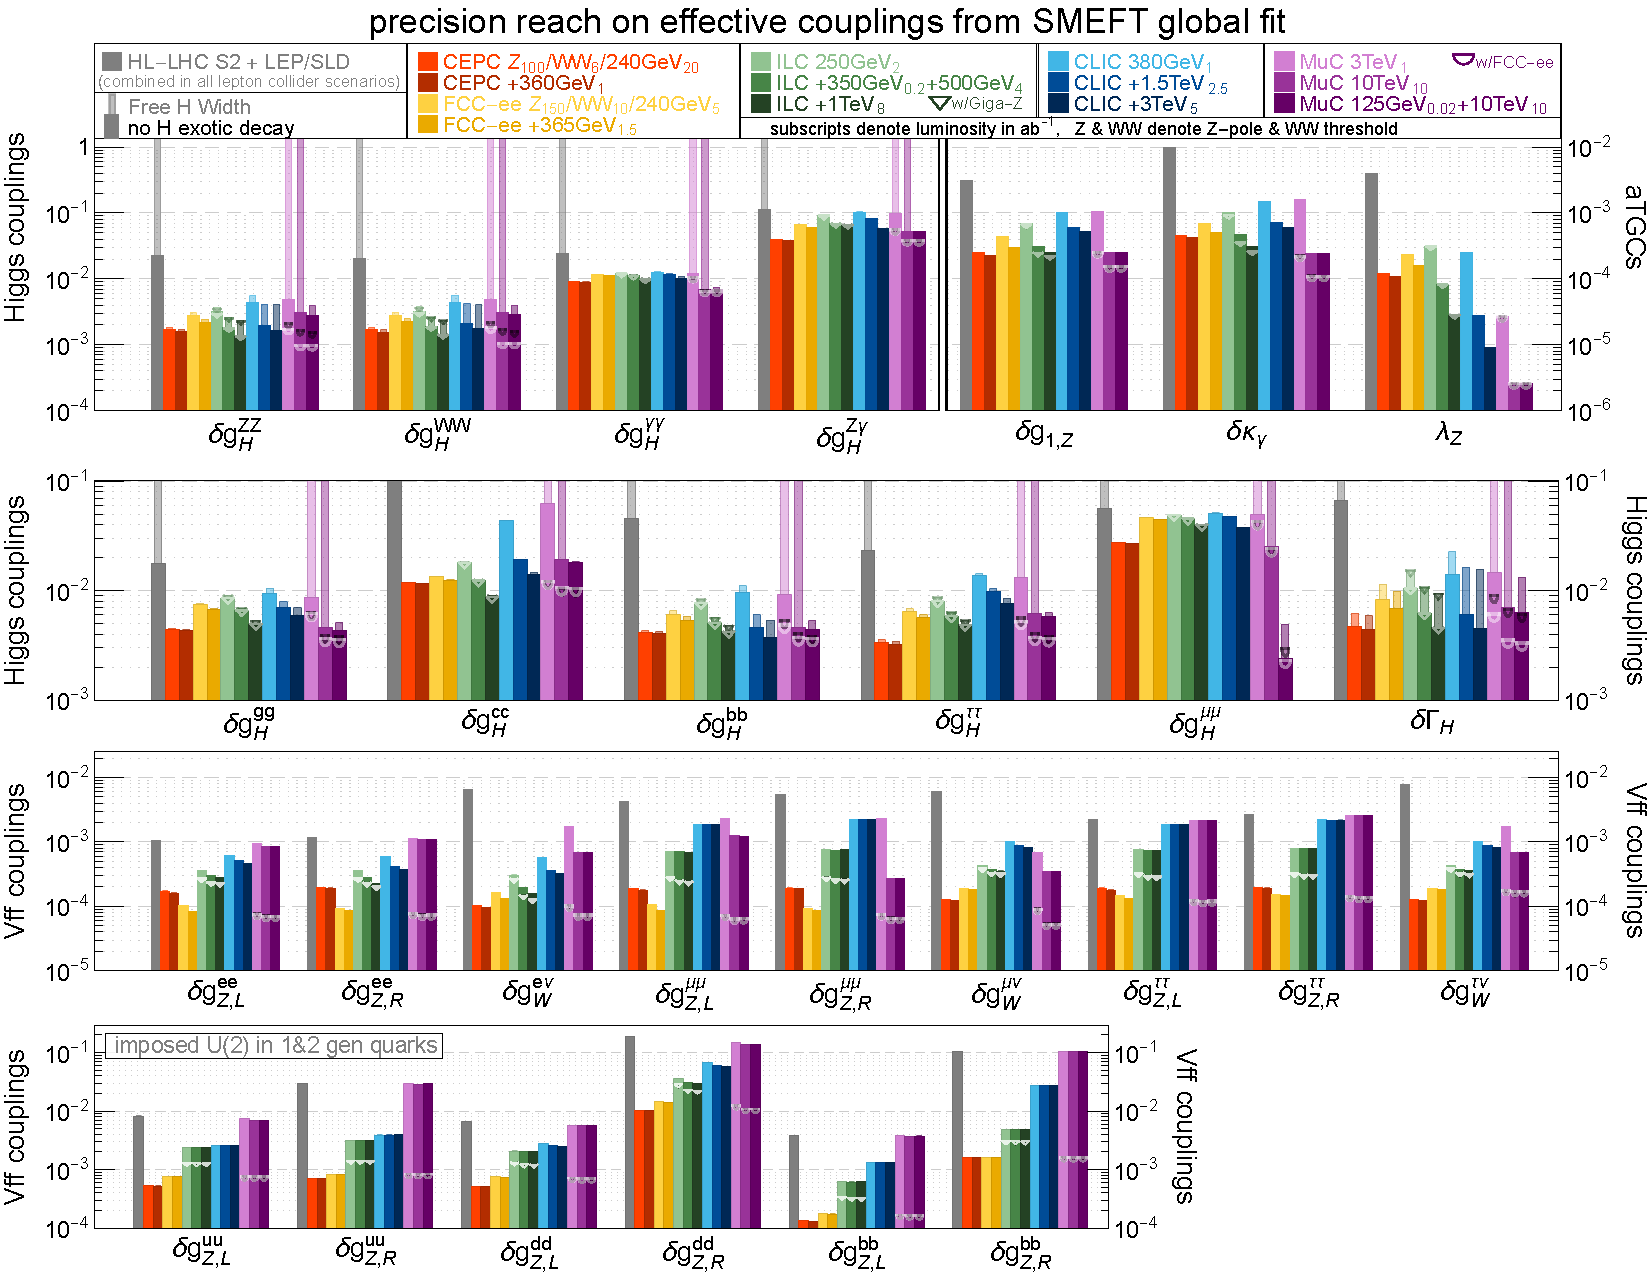
\includegraphics[width=0.92\textwidth]{Figs/Global_Interpretations/barplotsnow-xo1-smpar.pdf}
  \caption{Comparison of projected precision in a global interpretation framework. Source: Ref.~\cite{ECFAFactories2025}.}
  \label{fig:smeft-bar}
\end{figure}
The key lesson is that a projection is meaningful only after the measured observable, the assumptions entering its extraction, and the dominant uncertainty sources have been identified.

\subsection{Why global fits are necessary}
A single Wilson coefficient can affect many observables, and a single observable can depend on many Wilson coefficients. For example, the same operator that shifts a Higgs coupling may also shift a Z-pole coupling or a diboson distribution. Therefore a one-observable interpretation is generally not stable. A global fit is a statistical procedure in which the full observable vector
\begin{equation}
  \vec O = (\mZ,\gZ,\sintw,\mW,\sigma_{ZH},\BR(H\to b\bar b),\ldots)
\end{equation}
is compared with theory predictions that depend on a vector of coefficients,
\begin{equation}
  \vec C=(C_{\phi D},C_{\phi\Box},C_{\phi WB},C_{\phi q}^{(1)},C_{\ell\ell},\ldots) .
\end{equation}
The covariance matrix is essential because correlated systematic and theory uncertainties determine whether a deviation appears as a single-channel anomaly or a coherent pattern.

\begin{definition}{Flat direction}{flat-direction}
A flat direction is a linear combination of parameters that leaves the available observables approximately unchanged. New observables or measurements at different energies can lift flat directions by probing different combinations of the same Wilson coefficients.
\end{definition}

Figure~\ref{fig:smeft-quadratic} is used here as a visual anchor for the surrounding discussion. The important point is not only the numerical projection shown in the figure, but also the way in which the relevant FCC observable is connected to a physical parameter of the Standard Model or to a possible deviation from it.
\begin{figure}[H]
  \centering
  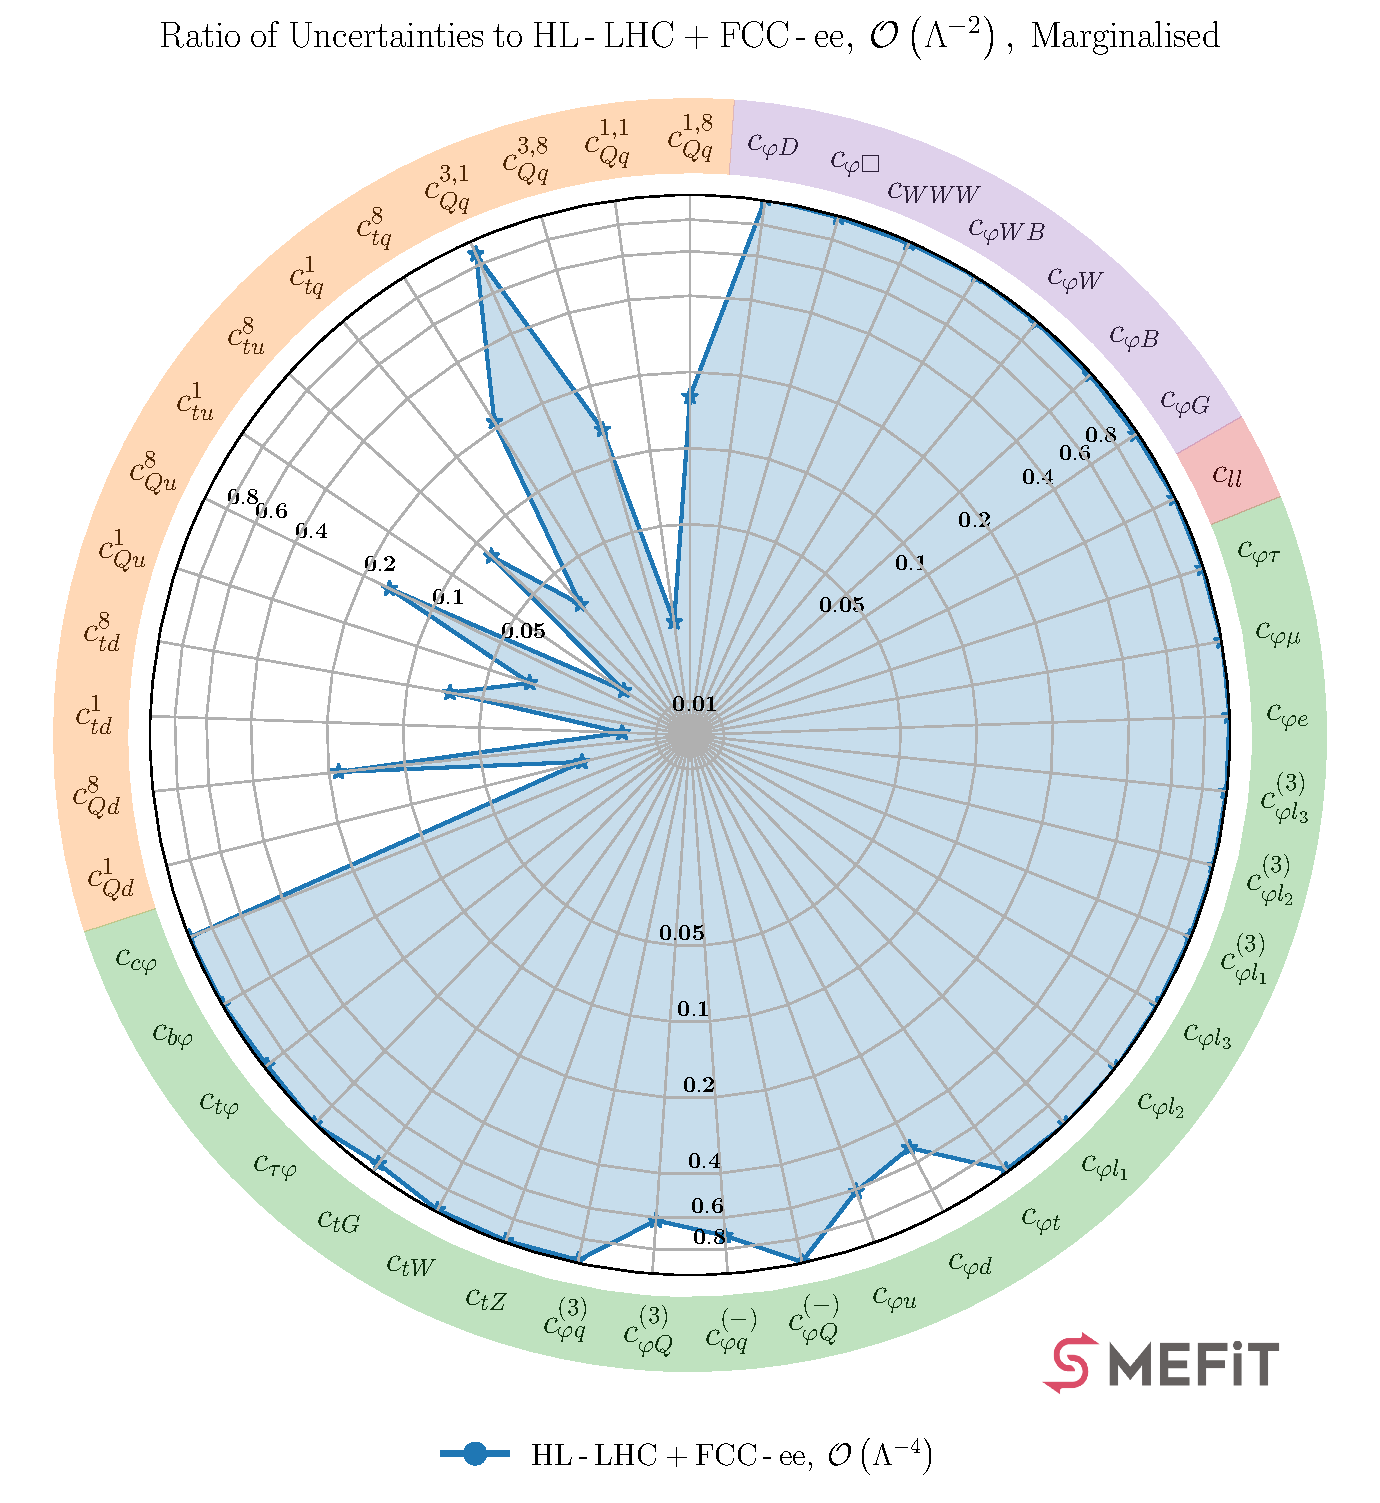
\includegraphics[width=0.88\textwidth]{Figs/Global_Interpretations/spider_plot_Quad_Effects.pdf}
  \caption{Spider plot illustrating the impact of quadratic EFT contributions in global fits. Source: Ref.~\cite{ArmadilloSMEFiT2026}.}
  \label{fig:smeft-quadratic}
\end{figure}
The key lesson is that a projection is meaningful only after the measured observable, the assumptions entering its extraction, and the dominant uncertainty sources have been identified.

Figure~\ref{fig:smeft-uv-spider} is used here as a visual anchor for the surrounding discussion. The important point is not only the numerical projection shown in the figure, but also the way in which the relevant FCC observable is connected to a physical parameter of the Standard Model or to a possible deviation from it.
\begin{figure}[H]
  \centering
  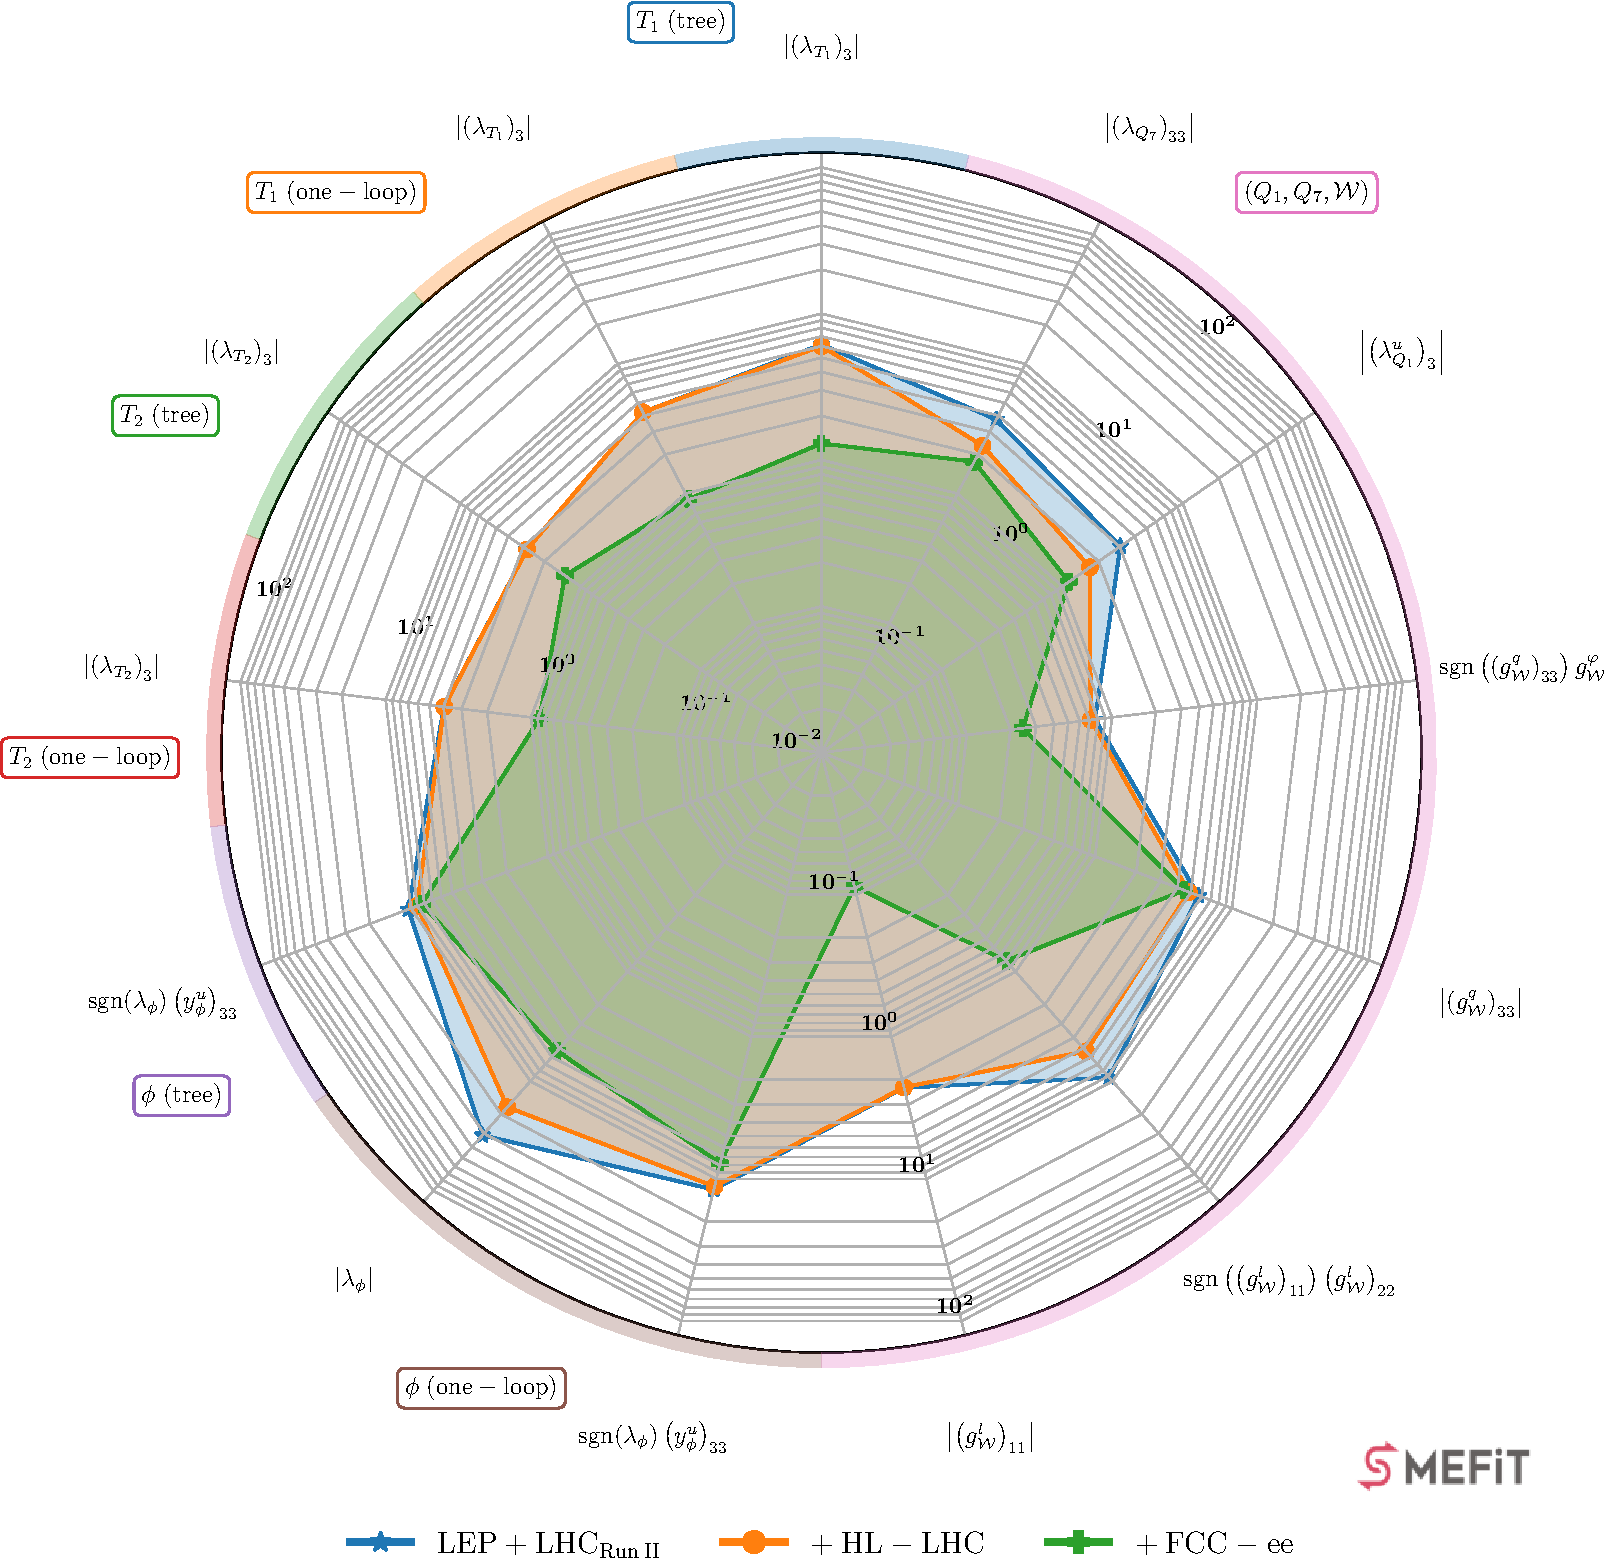
\includegraphics[width=0.88\textwidth]{Figs/Global_Interpretations/spider_plot_uv.pdf}
  \caption{FCC-ee constraints on representative UV models matched onto the SMEFT. Source: Ref.~\cite{ArmadilloSMEFiT2026}.}
  \label{fig:smeft-uv-spider}
\end{figure}
The key lesson is that a projection is meaningful only after the measured observable, the assumptions entering its extraction, and the dominant uncertainty sources have been identified.

\subsection{From Wilson coefficients to mass reach}
For a UV model with a coupling \(g_*\) and a mass \(M\), integrating out the heavy state may generate
\begin{equation}
  \frac{C_i}{\Lambda^2}\sim \frac{g_*^2}{M^2}
\end{equation}
for a tree-level exchange, or
\begin{equation}
  \frac{C_i}{\Lambda^2}\sim \frac{g_*^2}{16\pi^2M^2}
\end{equation}
for a loop-level contribution. This relation explains why the same experimental constraint on a Wilson coefficient corresponds to different mass reaches depending on whether the effect is tree-level, loop-level, chirality-suppressed, flavour-suppressed, or generated only through running.

Figure~\ref{fig:new-scalars} is used here as a visual anchor for the surrounding discussion. The important point is not only the numerical projection shown in the figure, but also the way in which the relevant FCC observable is connected to a physical parameter of the Standard Model or to a possible deviation from it.
\begin{figure}[H]
  \centering
  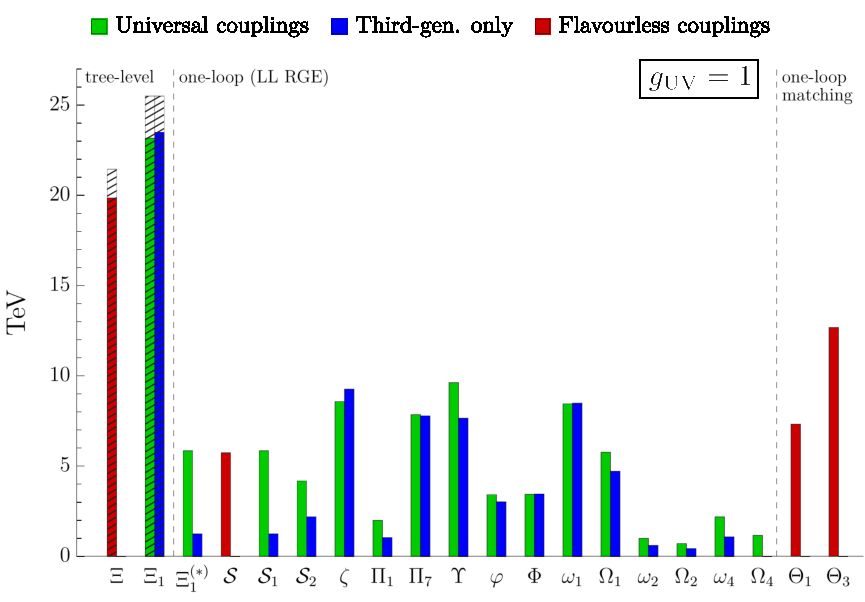
\includegraphics[width=0.88\textwidth]{Figs/Global_Interpretations/newscalars.pdf}
  \caption{Mass reach for representative new scalar fields inferred from precision observables and SMEFT matching. Source: Ref.~\cite{ECFAFactories2025}.}
  \label{fig:new-scalars}
\end{figure}
The key lesson is that a projection is meaningful only after the measured observable, the assumptions entering its extraction, and the dominant uncertainty sources have been identified.

Figure~\ref{fig:new-fermions} is used here as a visual anchor for the surrounding discussion. The important point is not only the numerical projection shown in the figure, but also the way in which the relevant FCC observable is connected to a physical parameter of the Standard Model or to a possible deviation from it.
\begin{figure}[H]
  \centering
  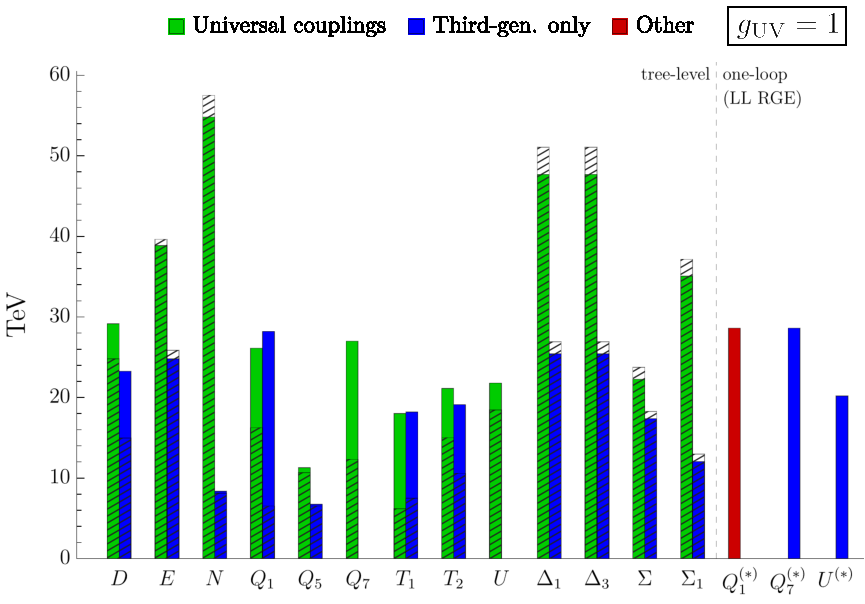
\includegraphics[width=0.88\textwidth]{Figs/Global_Interpretations/newfermions.pdf}
  \caption{Mass reach for representative new fermion fields inferred from precision observables and SMEFT matching. Source: Ref.~\cite{ECFAFactories2025}.}
  \label{fig:new-fermions}
\end{figure}
The key lesson is that a projection is meaningful only after the measured observable, the assumptions entering its extraction, and the dominant uncertainty sources have been identified.

Figure~\ref{fig:new-vectors} is used here as a visual anchor for the surrounding discussion. The important point is not only the numerical projection shown in the figure, but also the way in which the relevant FCC observable is connected to a physical parameter of the Standard Model or to a possible deviation from it.
\begin{figure}[H]
  \centering
  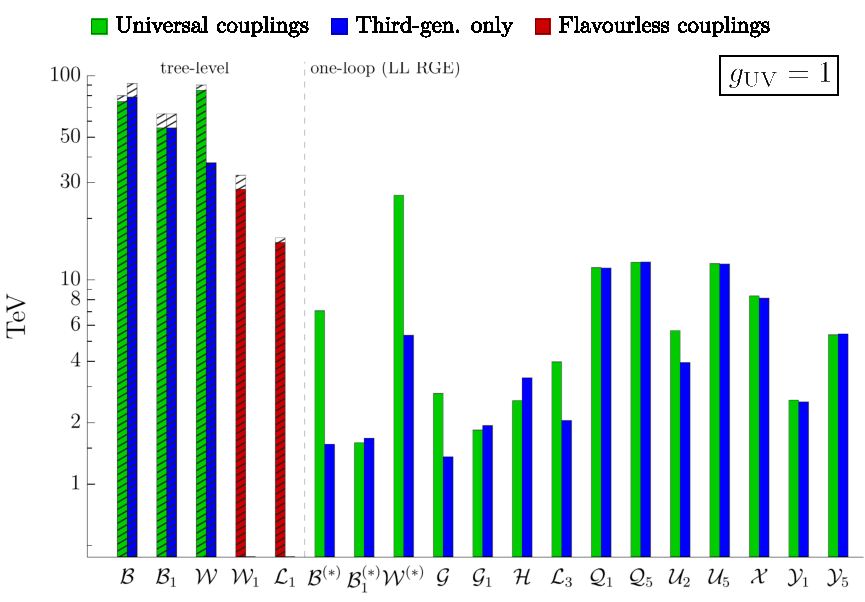
\includegraphics[width=0.88\textwidth]{Figs/Global_Interpretations/newvectorslog.pdf}
  \caption{Mass reach for representative new vector fields inferred from precision observables and SMEFT matching. Source: Ref.~\cite{ECFAFactories2025}.}
  \label{fig:new-vectors}
\end{figure}
The key lesson is that a projection is meaningful only after the measured observable, the assumptions entering its extraction, and the dominant uncertainty sources have been identified.

\begin{examplebox}{A one-operator estimate of mass reach}{mass-reach-example}
Assume an observable constrains \(|C/\Lambda^2|<1/(10\\,\TeV)^2\). A tree-level UV completion with \(g_*=1\) has a nominal reach \(M>10\\,\TeV\). If the same coefficient is loop-generated, the reach is reduced by roughly \(1/(4\pi)\), giving a mass scale of order \(M>0.8\\,\TeV\) for \(g_*=1\). This simple exercise is why UV matching information is needed before translating SMEFT bars into model statements.
\end{examplebox}

\begin{guidedchecksbox}
\begin{enumerate}[leftmargin=1.6em]
\item In Eq.~\eqref{eq:sigma-expansion}, identify the term that can be negative and the term that is positive semi-definite only in special cases.
\item Explain why including quadratic dimension-six terms may improve numerical sensitivity while also raising questions about dimension-eight effects.
\item Give an example of two FCC-ee measurements that can constrain related electroweak-current operators.
\end{enumerate}
\end{guidedchecksbox}

\subsection{Exercises}
\begin{enumerate}[leftmargin=1.6em]
\item Starting from Eq.~\eqref{eq:smeft-lagrangian-basic}, explain why dimension-six operators are usually the leading BSM correction if baryon and lepton number are conserved.
\item For a two-observable, two-parameter fit, sketch how a new measurement can rotate and shrink an error ellipse.
\item Explain why Z-pole, WW, Higgs and top data should not be interpreted in four independent EFT fits if the goal is a model-independent constraint.
\end{enumerate}


\newpage
\section{Higgs precision physics at FCC-ee}
\begin{guidelinebox}
The Higgs programme is the clearest example of why FCC-ee is more than a high-luminosity counting experiment. The clean initial state and the recoil method allow an inclusive Higgsstrahlung cross section to be measured without specifying the Higgs decay. This is the key step that converts relative Higgs rates into absolute couplings and a total-width determination.
\end{guidelinebox}

\subsection{Processes and learning goals}
The main Higgs production modes at FCC-ee are
\begin{align}
  e^+e^- &\to ZH, && \text{Higgsstrahlung, dominant near } 240\,\GeV,\\
  e^+e^- &\to \nu\bar\nu H, && \text{WW fusion, increasingly important at }365\,\GeV,\\
  e^+e^- &\to e^+e^-H, && \text{ZZ fusion, smaller but conceptually related}.
\end{align}
The main decay modes entering coupling fits include
\begin{equation}
  H\to b\bar b,\ c\bar c,\ gg,\ WW^*,\ ZZ^*,\tau^+\tau^-,\mu^+\mu^-,\gamma\gamma,\ Z\gamma,\ \text{invisible},\ \text{exotic}.
\end{equation}
The reader should understand how measurements of \(\sigma_{ZH}\), \(\sigma_{ZH}\times\BR(H\to X)\), and \(\sigma_{\nu\bar\nu H}\times\BR(H\to X)\) are combined to extract absolute Higgs couplings.

Figure~\ref{fig:higgsstrahlung} is used here as a visual anchor for the surrounding discussion. The important point is not only the numerical projection shown in the figure, but also the way in which the relevant FCC observable is connected to a physical parameter of the Standard Model or to a possible deviation from it.
\begin{figure}[H]
  \centering
  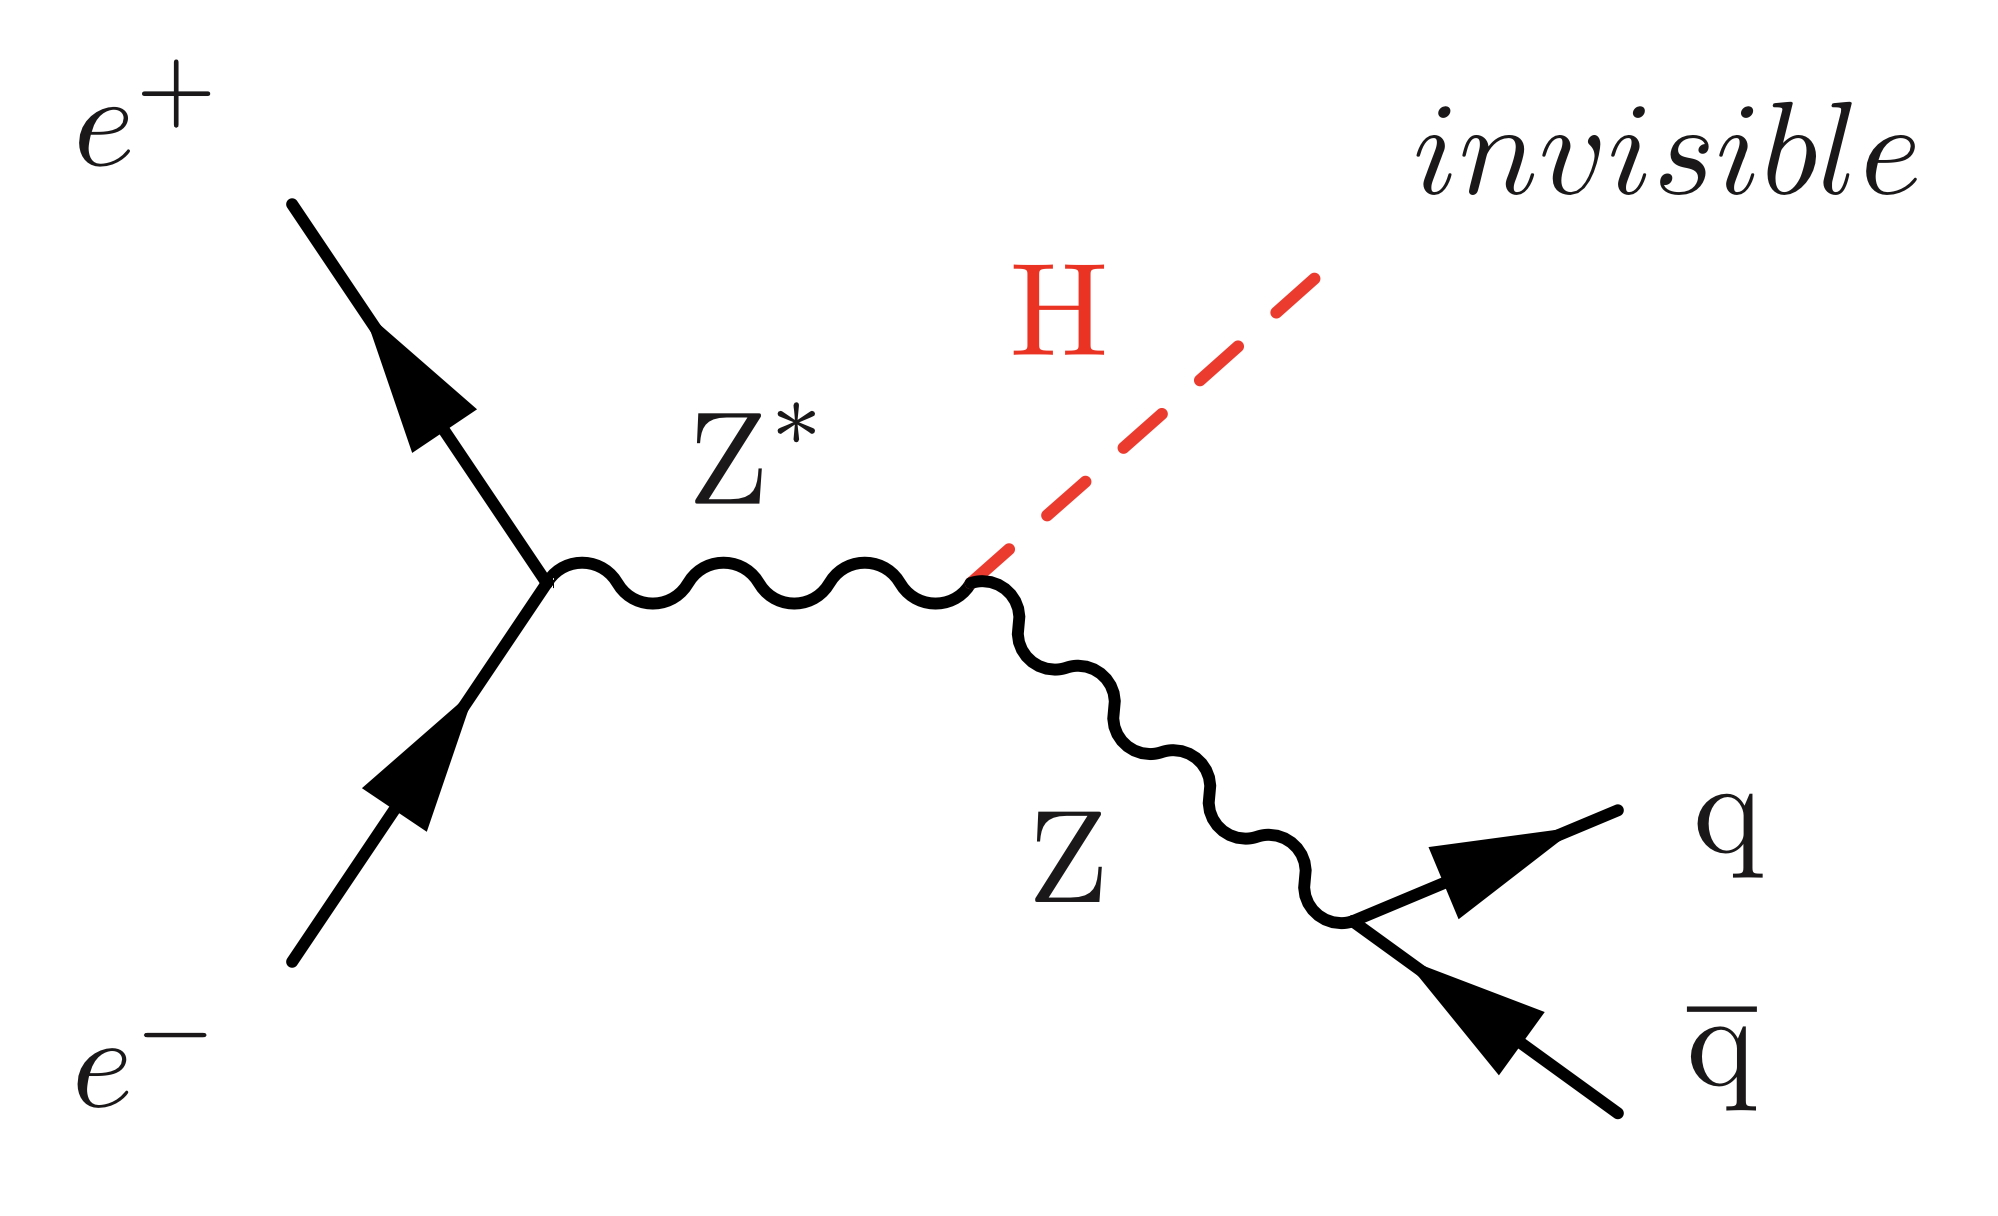
\includegraphics[width=0.70\textwidth]{Figs/Higgs/higgsstrahlung.jpg}
  \caption{Leading-order Higgsstrahlung process, \(e^+e^-\to ZH\), the central production mode for model-independent Higgs measurements at 240 GeV. Source: Ref.~\cite{ECFAFactories2025}.}
  \label{fig:higgsstrahlung}
\end{figure}
The key lesson is that a projection is meaningful only after the measured observable, the assumptions entering its extraction, and the dominant uncertainty sources have been identified.

\begin{definition}{Higgsstrahlung}{higgsstrahlung}
Higgsstrahlung is the associated production process \(e^+e^-\to ZH\). At FCC-ee it is the primary Higgs process at \(\sqrt{s}=240\\,\GeV\). It is especially powerful because the Z boson can be reconstructed and used to infer the Higgs recoil system independently of the Higgs decay.
\end{definition}

\subsection{The recoil-mass method}
Consider the process
\begin{equation}
  e^+(p_1)+e^-(p_2)\to Z(k)+H(q),
\end{equation}
with total incoming momentum \(P=p_1+p_2\) and \(P^2=s\). The recoil momentum is \(q=P-k\), hence
\begin{equation}
  m_{\rm rec}^2 = q^2 = (P-k)^2=s+m_Z^2-2P\cdot k .
\end{equation}
In the centre-of-mass frame, \(P=(\sqrt{s},\vec 0)\), giving
\begin{equation}
  m_{\rm rec}^2=s+m_Z^2-2\sqrt{s}E_Z .
  \label{eq:recoil-mass}
\end{equation}
Equation~\eqref{eq:recoil-mass} is one of the defining formulas of a lepton-collider Higgs factory. It allows the inclusive process \(e^+e^-\to ZH\) to be counted using only the reconstructed Z boson.

Figure~\ref{fig:higgs-recoil} is used here as a visual anchor for the surrounding discussion. The important point is not only the numerical projection shown in the figure, but also the way in which the relevant FCC observable is connected to a physical parameter of the Standard Model or to a possible deviation from it.
\begin{figure}[H]
  \centering
  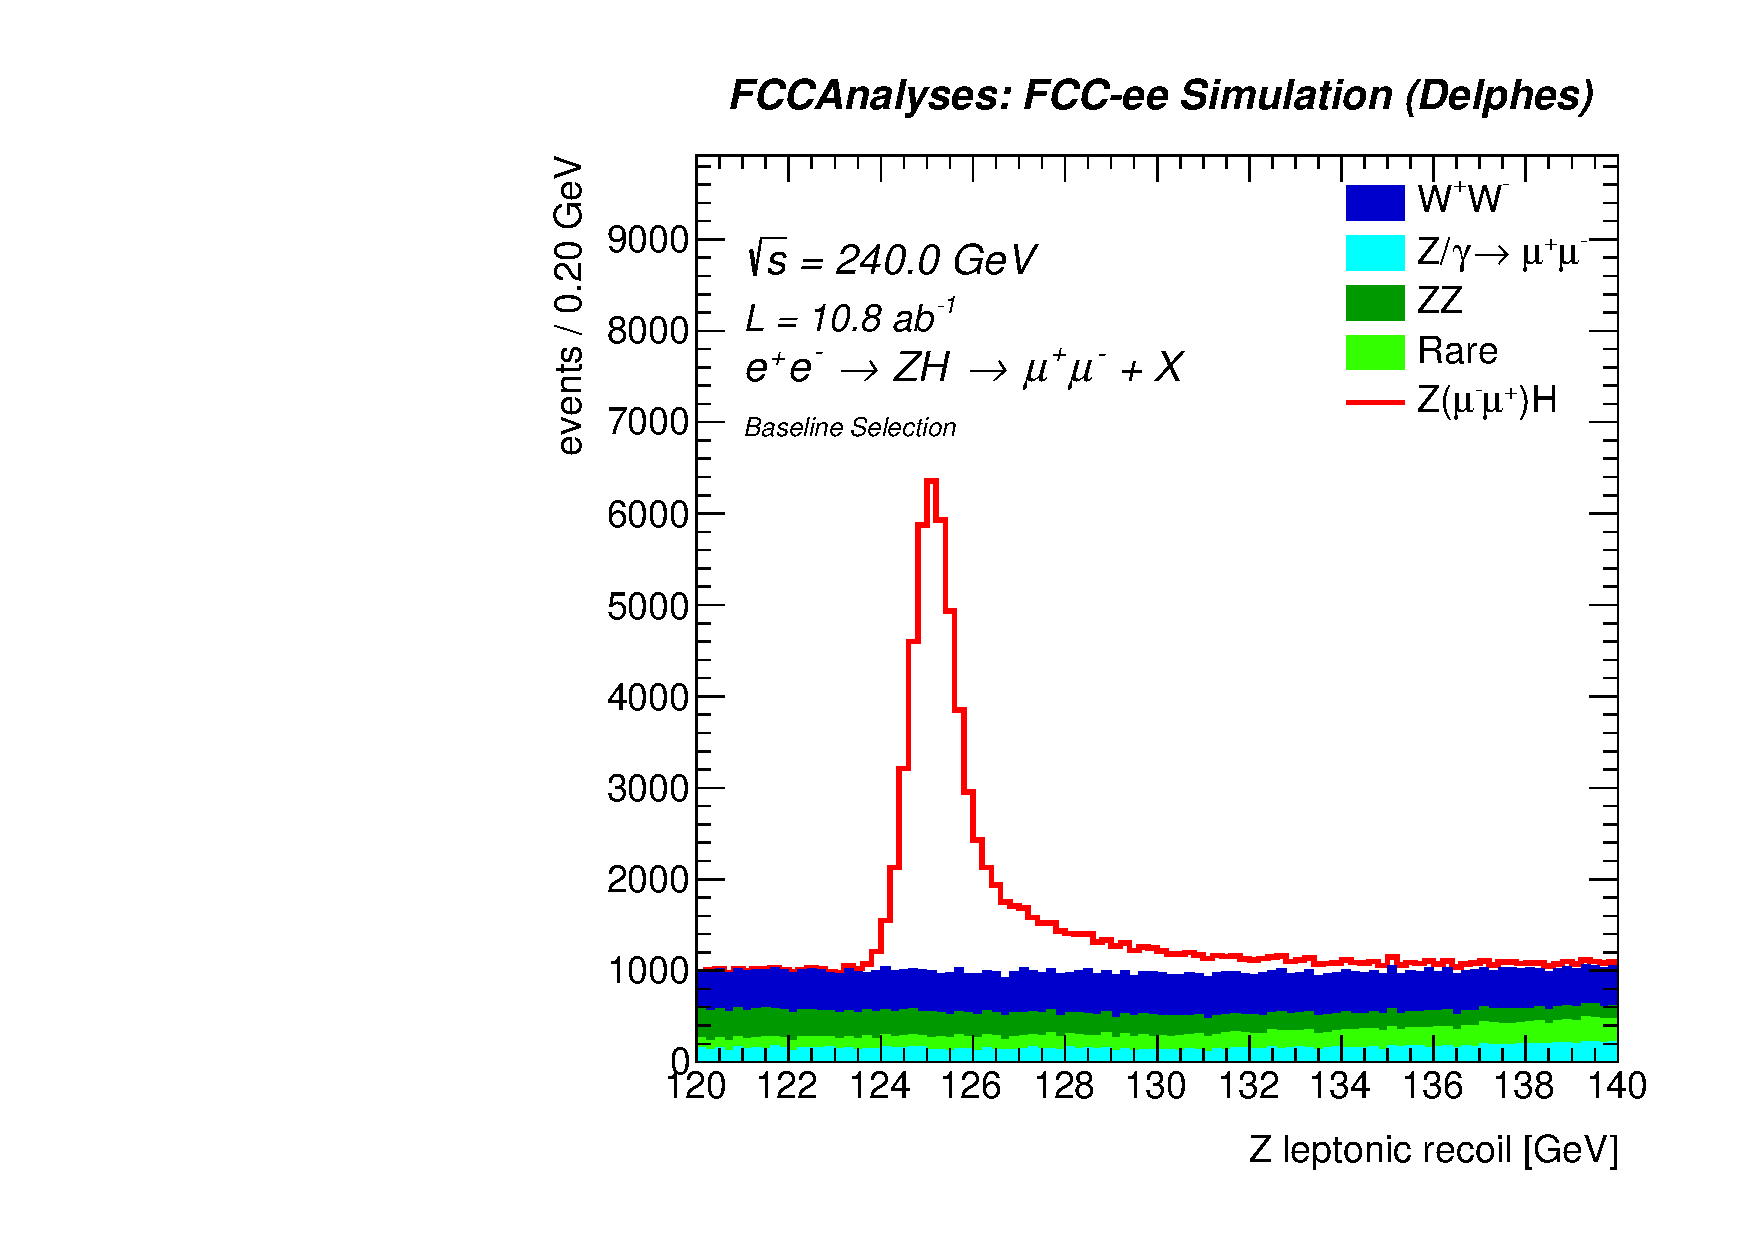
\includegraphics[width=0.78\textwidth]{Figs/Higgs/recoil.pdf}
  \caption{Representative recoil-mass distribution after selections in \(e^+e^-\to ZH\) at \(\sqrt{s}=240\,\GeV\). The peak position and normalisation encode the Higgs mass and inclusive \(ZH\) rate. Source: Ref.~\cite{ECFAFactories2025}.}
  \label{fig:higgs-recoil}
\end{figure}
The key lesson is that a projection is meaningful only after the measured observable, the assumptions entering its extraction, and the dominant uncertainty sources have been identified.

Figure~\ref{fig:recoz-mass} is used here as a visual anchor for the surrounding discussion. The important point is not only the numerical projection shown in the figure, but also the way in which the relevant FCC observable is connected to a physical parameter of the Standard Model or to a possible deviation from it.
\begin{figure}[H]
  \centering
  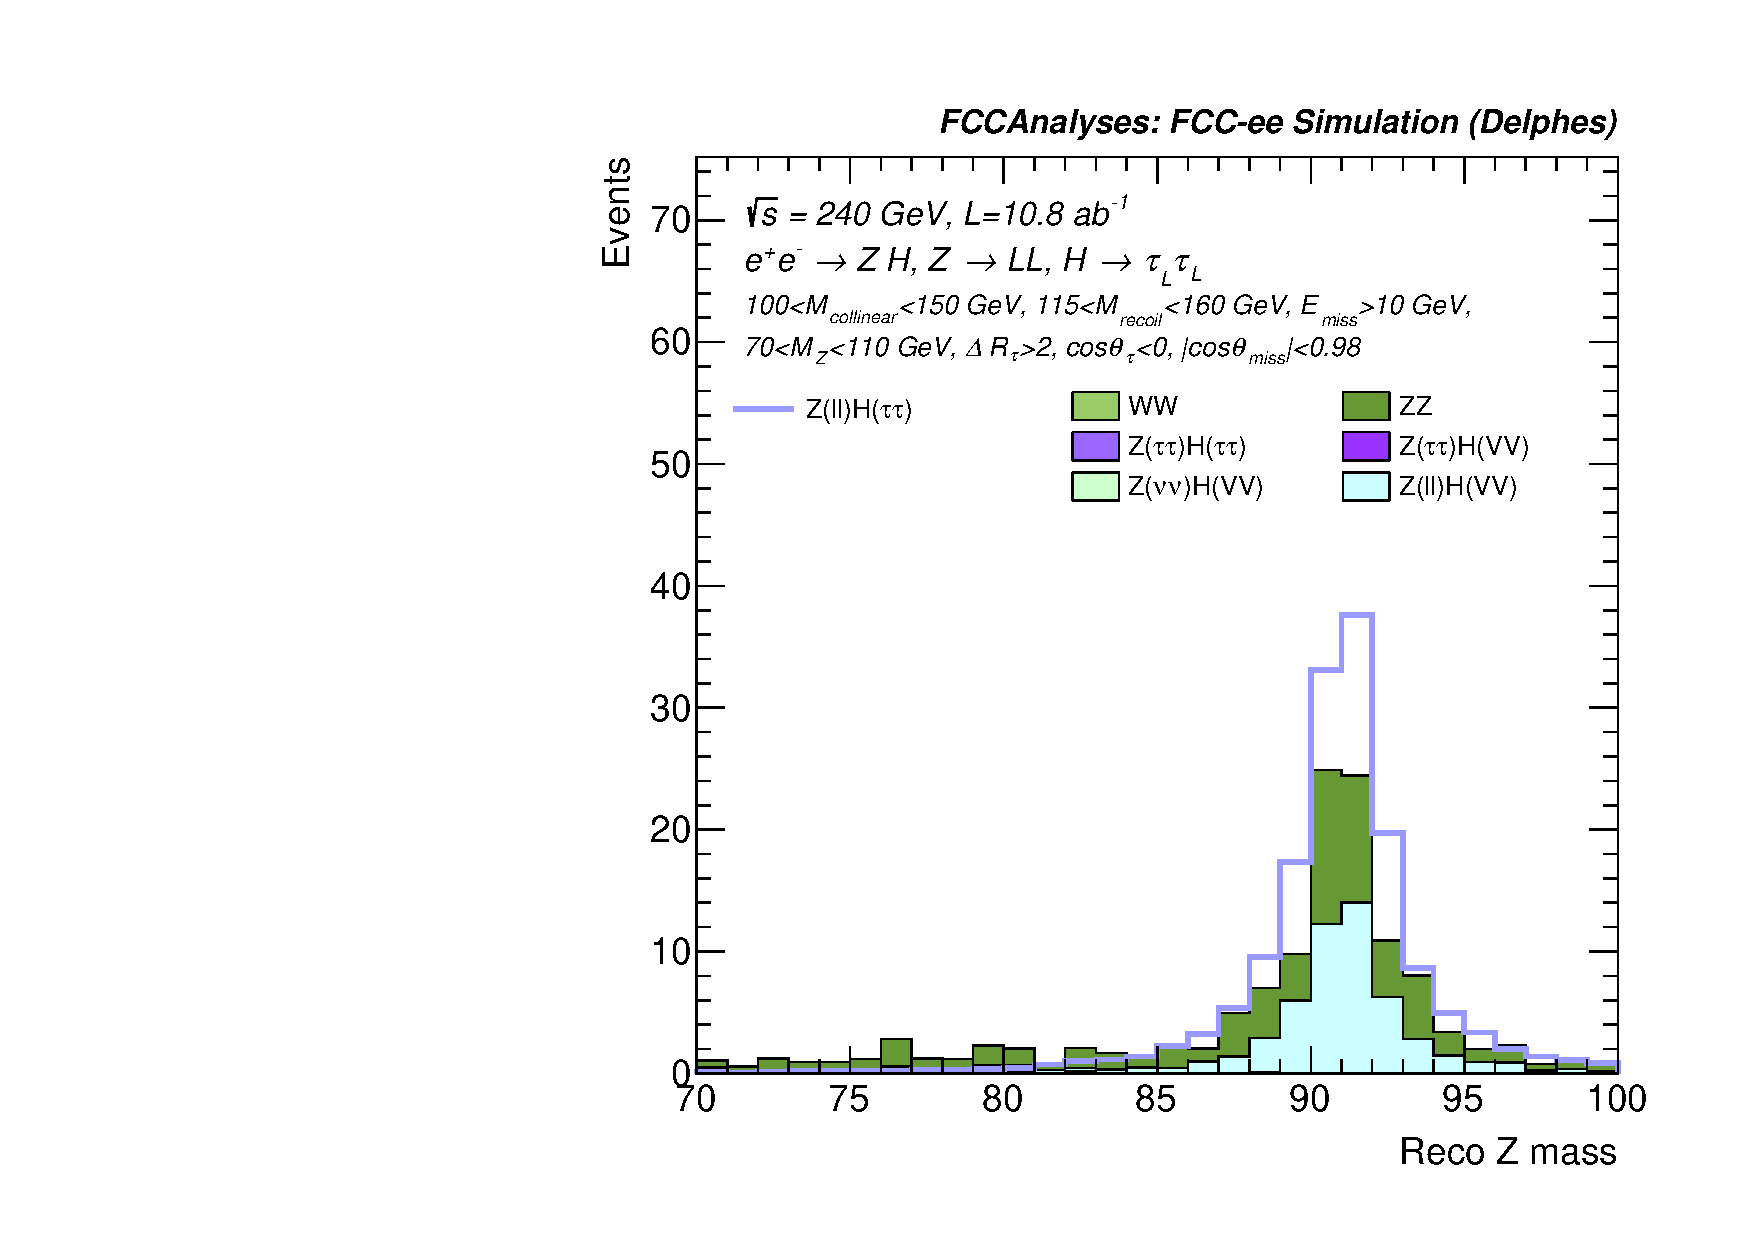
\includegraphics[width=0.75\textwidth]{Figs/Higgs/RecoZ_mass.pdf}
  \caption{Reconstructed Z-boson mass distribution used in Higgsstrahlung selections. Source: Ref.~\cite{ECFAFactories2025}.}
  \label{fig:recoz-mass}
\end{figure}
The key lesson is that a projection is meaningful only after the measured observable, the assumptions entering its extraction, and the dominant uncertainty sources have been identified.

\begin{examplebox}{Deriving the recoil mass}{recoil-derivation}
Starting with four-momentum conservation, \(q=P-k\). Squaring gives \(q^2=P^2+k^2-2P\cdot k\). Since \(P^2=s\), \(k^2=m_Z^2\), and \(P\cdot k=\sqrt{s}E_Z\) in the centre-of-mass frame, Eq.~\eqref{eq:recoil-mass} follows. The important point is that the Higgs decay products never entered the derivation.
\end{examplebox}

\subsection{From rates to couplings}
At leading order, the inclusive Higgsstrahlung cross section is proportional to the square of the \(HZZ\) coupling,
\begin{equation}
  \sigma_{ZH}\propto g_{HZZ}^2 .
\end{equation}
Exclusive rates measure products of production and decay factors divided by the total width,
\begin{equation}
  \sigma_{ZH}\times \BR(H\to X)
  \propto
  \frac{g_{HZZ}^2 g_{HXX}^2}{\Gamma_H} .
  \label{eq:zh-rate-couplings}
\end{equation}
Similarly, WW fusion gives
\begin{equation}
  \sigma_{\nu\bar\nu H}\times \BR(H\to X)
  \propto
  \frac{g_{HWW}^2 g_{HXX}^2}{\Gamma_H} .
  \label{eq:wwfusion-rate-couplings}
\end{equation}
The pair of Eqs.~\eqref{eq:zh-rate-couplings} and~\eqref{eq:wwfusion-rate-couplings} explains why the 240 GeV and 365 GeV runs are complementary: the first fixes the absolute \(ZH\) normalisation, while the second strengthens the WW-fusion lever arm and hence the width extraction.

\begin{definition}{Signal strength}{signal-strength}
For a production mode \(i\) and decay final state \(f\), the signal strength is \(\mu_i^f=(\sigma_i\BR_f)/(\sigma_i\BR_f)_{\rm SM}\). At hadron colliders it is often the natural Higgs observable. At FCC-ee, the recoil measurement makes it possible to go beyond signal strengths and determine absolute normalisations.
\end{definition}

Figure~\ref{fig:higgs-couplings} is used here as a visual anchor for the surrounding discussion. The important point is not only the numerical projection shown in the figure, but also the way in which the relevant FCC observable is connected to a physical parameter of the Standard Model or to a possible deviation from it.
\begin{figure}[H]
  \centering
  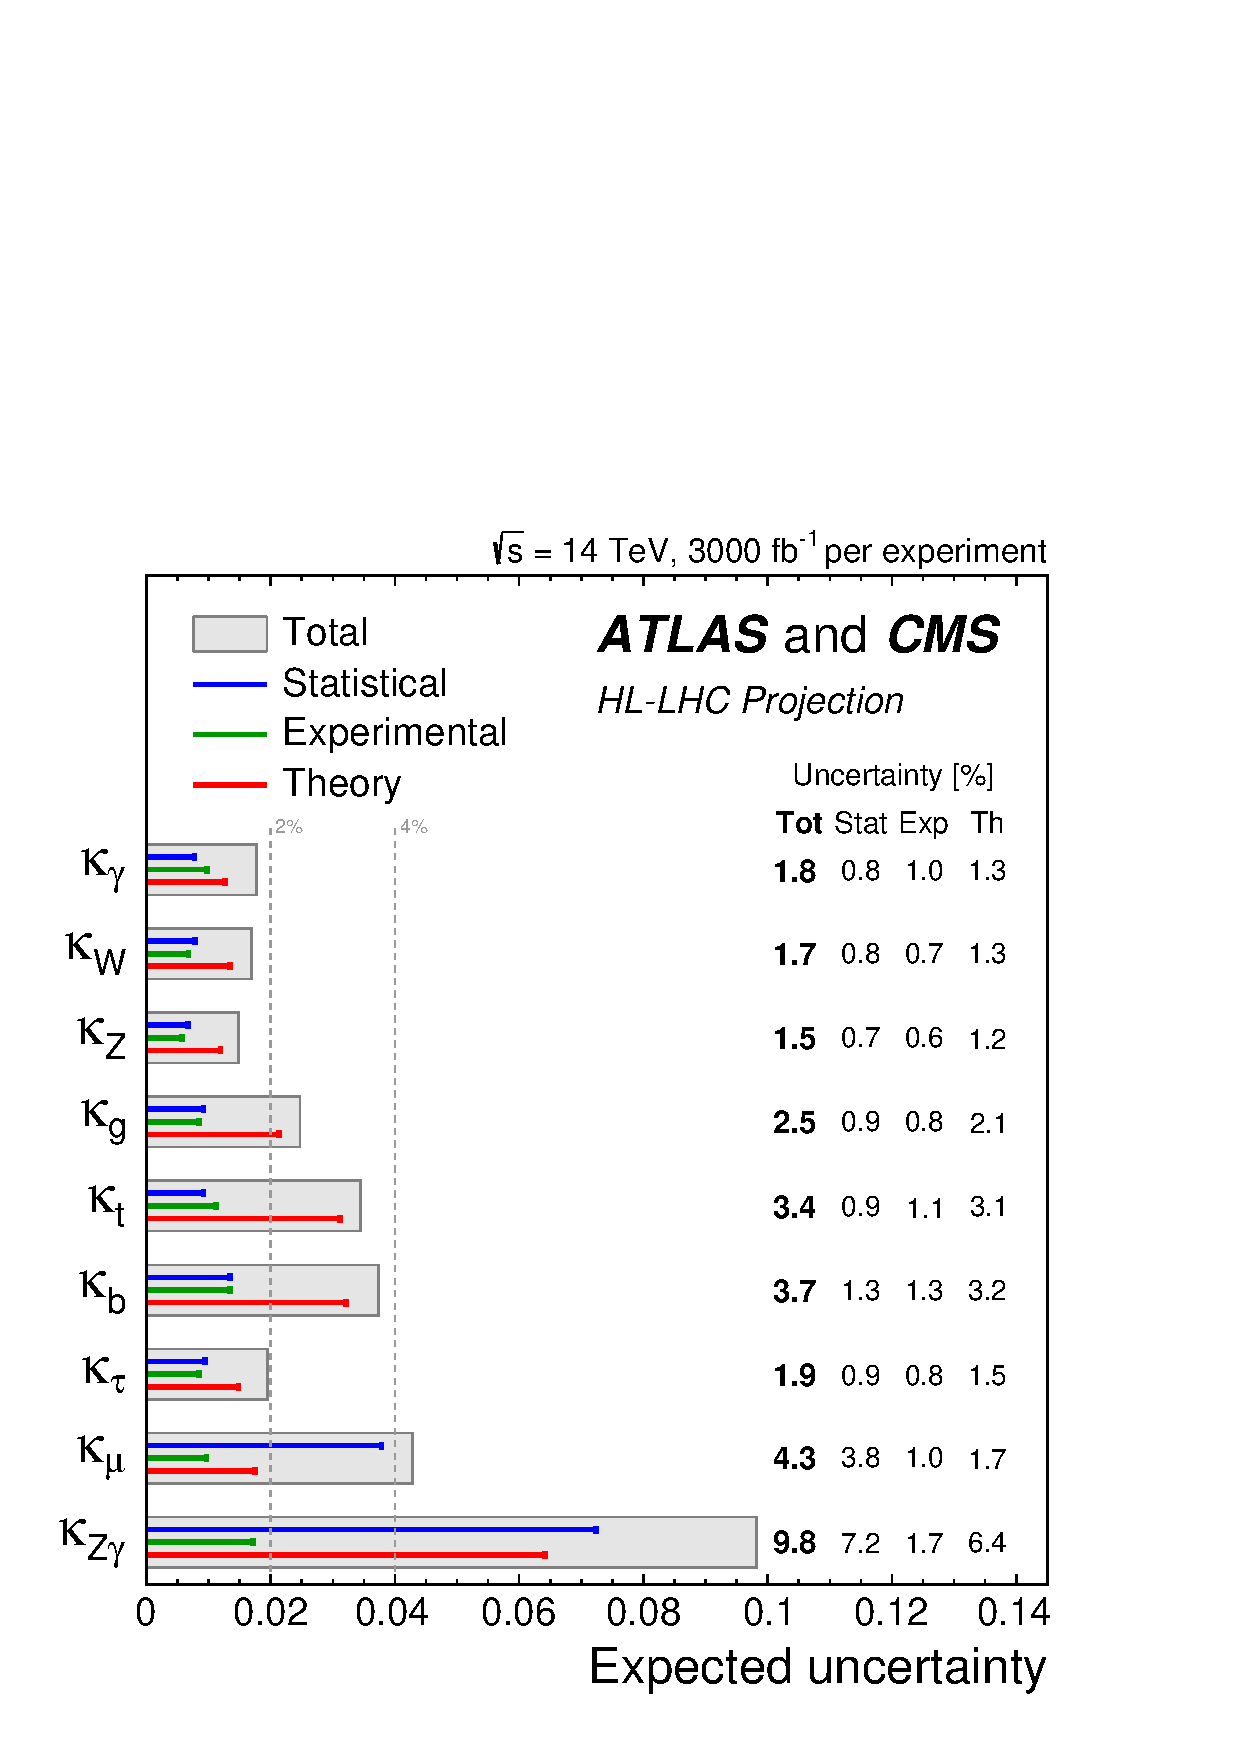
\includegraphics[width=0.88\textwidth]{Figs/Higgs/ATLAS_CMS_Higgs_couplings.pdf}
  \caption{Comparison of Higgs coupling precision projections, illustrating the transition from LHC-style rate measurements to lepton-collider absolute coupling determinations. Source: Ref.~\cite{ECFAFactories2025}.}
  \label{fig:higgs-couplings}
\end{figure}
The key lesson is that a projection is meaningful only after the measured observable, the assumptions entering its extraction, and the dominant uncertainty sources have been identified.

\begin{table}[H]
\centering
\small
\caption{Representative 68\% CL Higgs-coupling projections in the FCC Feasibility Study baseline. The FCC-ee column assumes combination with HL-LHC where indicated in the source table; the last column illustrates the gain from the integrated FCC-ee+FCC-hh programme. Values are relative uncertainties unless stated otherwise. Source: Ref.~\cite{FCCFSRVol1}.}
\label{tab:higgs-projection-benchmarks}
\begin{tabular}{@{}lcc@{}}
\toprule
Quantity & FCC-ee & FCC-ee+FCC-hh \\
\midrule
\(\kappa_Z\) & 0.10\% & 0.10\% \\
\(\kappa_W\) & 0.29\% & 0.25\% \\
\(\kappa_b\) & 0.38/0.49\% & 0.33/0.45\% \\
\(\kappa_c\) & 0.70/0.87\% & 0.68/0.85\% \\
\(\kappa_\tau\) & 0.46\% & 0.40\% \\
\(\kappa_g\) & 0.49/0.54\% & 0.41/0.44\% \\
\(\kappa_\gamma\) & 1.1\% & 0.30\% \\
\(\kappa_{Z\gamma}\) & 4.3\% & 0.67\% \\
\(\kappa_t\) & 3.1\% & 0.75\% \\
\(\Gamma_H\) & 0.78\% & 0.69\% \\
\(\BR_{\rm inv}\) 95\% CL upper limit & \(5\times10^{-4}\) & \(2.3\times10^{-4}\) \\
\(\BR_{\rm unt}\) 95\% CL upper limit & \(6.8\times10^{-3}\) & \(6.7\times10^{-3}\) \\
\bottomrule
\end{tabular}
\end{table}
The slash in some entries indicates the impact of projected Standard Model parametric uncertainties, for example from heavy-quark masses. The table is therefore also a useful reminder that sub-percent Higgs physics is limited not only by event counts but also by external inputs and theory assumptions.

Figure~\ref{fig:higgs-fermion-eff} is used here as a visual anchor for the surrounding discussion. The important point is not only the numerical projection shown in the figure, but also the way in which the relevant FCC observable is connected to a physical parameter of the Standard Model or to a possible deviation from it.
\begin{figure}[H]
  \centering
  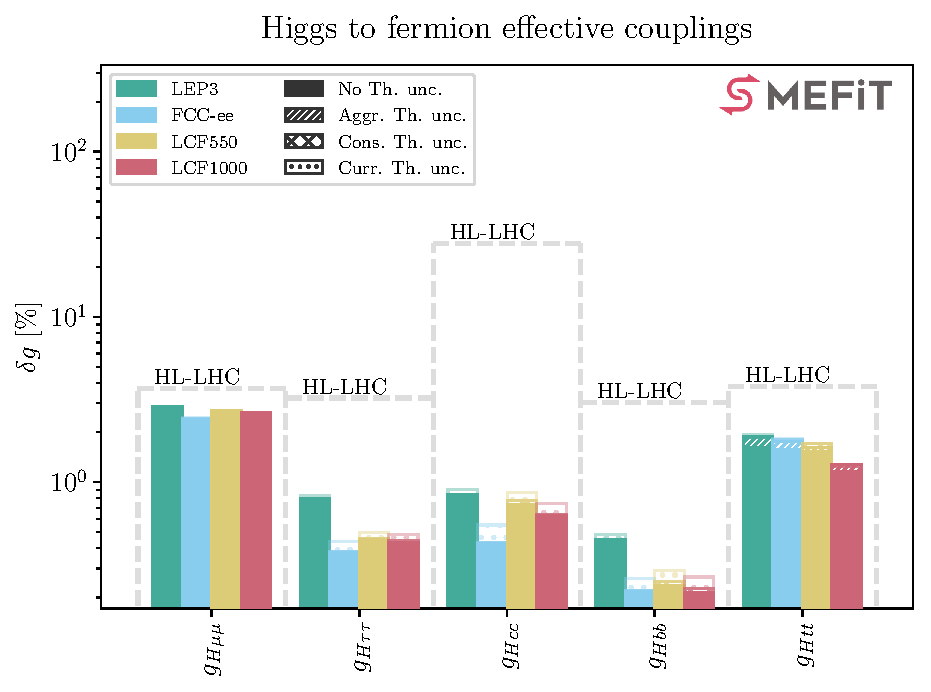
\includegraphics[width=0.78\textwidth]{Figs/Higgs_to_fermion_effective_couplings.pdf}
  \caption{Projected constraints on effective Higgs couplings to fermions. Source: Ref.~\cite{ArmadilloSMEFiT2026}.}
  \label{fig:higgs-fermion-eff}
\end{figure}
The key lesson is that a projection is meaningful only after the measured observable, the assumptions entering its extraction, and the dominant uncertainty sources have been identified.

Figure~\ref{fig:higgs-vector-eff} is used here as a visual anchor for the surrounding discussion. The important point is not only the numerical projection shown in the figure, but also the way in which the relevant FCC observable is connected to a physical parameter of the Standard Model or to a possible deviation from it.
\begin{figure}[H]
  \centering
  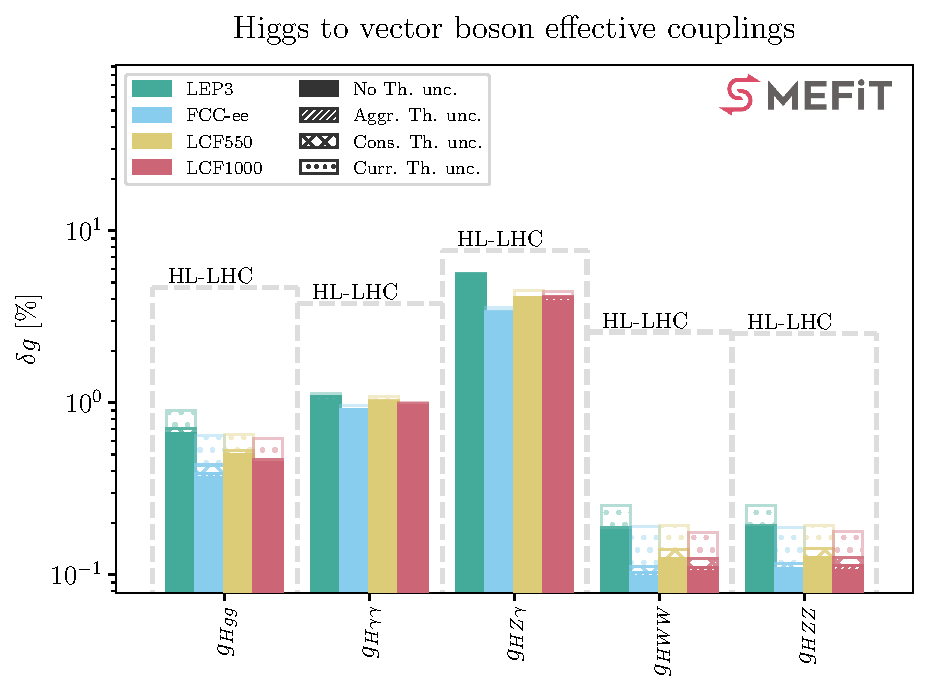
\includegraphics[width=0.78\textwidth]{Figs/Higgs_to_vector_boson_effective_couplings.pdf}
  \caption{Projected constraints on effective Higgs couplings to electroweak vector bosons. Source: Ref.~\cite{ArmadilloSMEFiT2026}.}
  \label{fig:higgs-vector-eff}
\end{figure}
The key lesson is that a projection is meaningful only after the measured observable, the assumptions entering its extraction, and the dominant uncertainty sources have been identified.

\subsection{The total Higgs width}
The Standard Model Higgs width is too narrow to be resolved directly in a lineshape measurement at 125 GeV. Instead it is inferred from combinations of rates. A useful schematic relation is
\begin{equation}
  \Gamma_H \sim \frac{\Gamma(H\to WW^*)}{\BR(H\to WW^*)} .
\end{equation}
In practice, the extraction is done in a global fit using \(ZH\), WW fusion and branching-ratio measurements. The recoil measurement is crucial because it gives an inclusive normalisation that does not assume a specific Higgs decay pattern.

\begin{guidedchecksbox}
\begin{enumerate}[leftmargin=1.6em]
\item Use Eq.~\eqref{eq:zh-rate-couplings} to explain why \(\sigma_{ZH}\times\BR(H\to b\bar b)\) alone does not determine \(g_{Hbb}\) without information on \(\Gamma_H\).
\item Explain why an invisible Higgs decay changes branching ratios but not the inclusive recoil count.
\item Describe how adding WW-fusion information helps break the width-coupling degeneracy.
\end{enumerate}
\end{guidedchecksbox}

\subsection{The kappa framework}
A compact way to report Higgs coupling sensitivities is the kappa framework,
\begin{equation}
  \kappa_i = \frac{g_i}{g_i^{\rm SM}} .
\end{equation}
For a production mode \(i\) and decay mode \(f\), the signal strength is
\begin{equation}
  \mu_i^f = \frac{\kappa_i^2\kappa_f^2}{\kappa_H^2},
  \qquad
  \kappa_H^2=\sum_f \kappa_f^2\BR_f^{\rm SM}
\end{equation}
if no invisible or untagged BSM decays are allowed. If additional Higgs decays are included, one may write schematically
\begin{equation}
  \Gamma_H = \frac{\kappa_H^2}{1-\BR_{\rm inv}-\BR_{\rm unt}}\Gamma_H^{\rm SM} .
  \label{eq:kappa-width-bsm}
\end{equation}
The kappa framework is intuitive, but it is not a complete EFT. It ignores momentum-dependent effects and gauge-invariance correlations that appear naturally in the SMEFT.

Figure~\ref{fig:kappa-universal} is used here as a visual anchor for the surrounding discussion. The important point is not only the numerical projection shown in the figure, but also the way in which the relevant FCC observable is connected to a physical parameter of the Standard Model or to a possible deviation from it.
\begin{figure}[H]
  \centering
  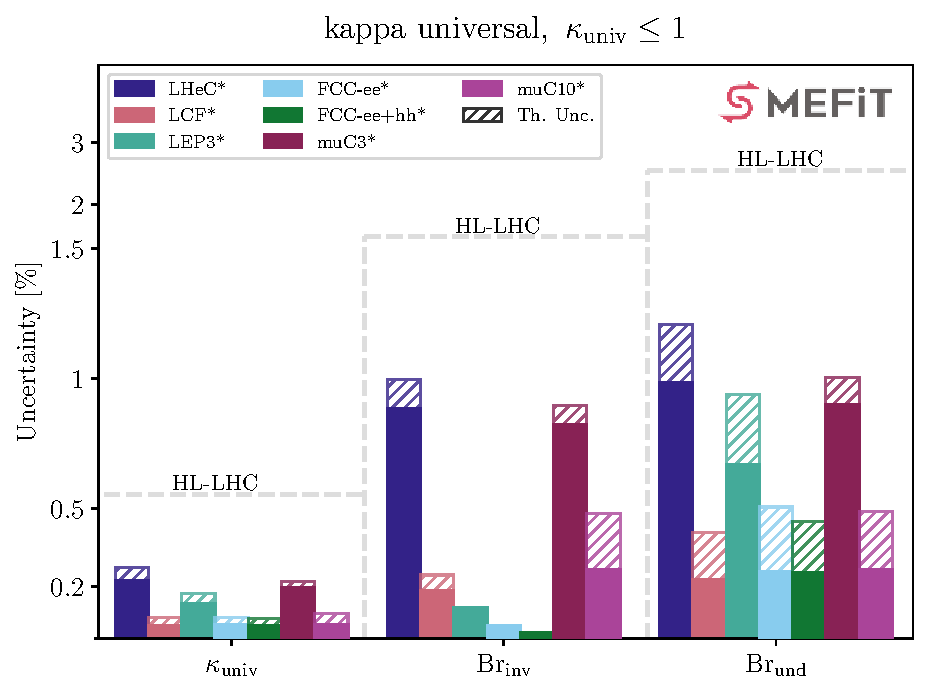
\includegraphics[width=0.78\textwidth]{Figs/kappa2025/k_universal.pdf}
  \caption{Example of a universal Higgs-coupling modifier interpretation. Source: Ref.~\cite{ArmadilloSMEFiT2026}.}
  \label{fig:kappa-universal}
\end{figure}
The key lesson is that a projection is meaningful only after the measured observable, the assumptions entering its extraction, and the dominant uncertainty sources have been identified.

\begin{remarkbox}{Kappa framework versus SMEFT}{kappa-vs-smeft}
The kappa framework is valuable for communicating projected Higgs precision, but it should not be confused with a model-independent quantum-field-theory interpretation. A shift in \(HZZ\) is generally correlated with shifts in electroweak observables, diboson processes and possibly fermionic currents. This is why Chapter~7 returns to SMEFT global fits.
\end{remarkbox}

\subsection{Higgs self-coupling}
The Higgs potential can be written as
\begin{equation}
  V(\Phi)=-\mu^2\Phi^\dagger\Phi+\lambda(\Phi^\dagger\Phi)^2 .
\end{equation}
After electroweak symmetry breaking, the physical Higgs field has cubic and quartic self-interactions,
\begin{equation}
  V(H)=\frac12 m_H^2H^2+\lambda_3 v H^3+\frac14\lambda_4H^4+\cdots .
\end{equation}
It is conventional to define
\begin{equation}
  \kappa_\lambda=\frac{\lambda_3}{\lambda_3^{\rm SM}} .
\end{equation}
FCC-ee can constrain \(\kappa_\lambda\) indirectly through loop effects in single-Higgs observables, while FCC-hh can probe it directly through double-Higgs production. The two approaches are complementary because they depend on different observables and different assumptions.

Figure~\ref{fig:hh-diagrams} is used here as a visual anchor for the surrounding discussion. The important point is not only the numerical projection shown in the figure, but also the way in which the relevant FCC observable is connected to a physical parameter of the Standard Model or to a possible deviation from it.
\begin{figure}[H]
  \centering
  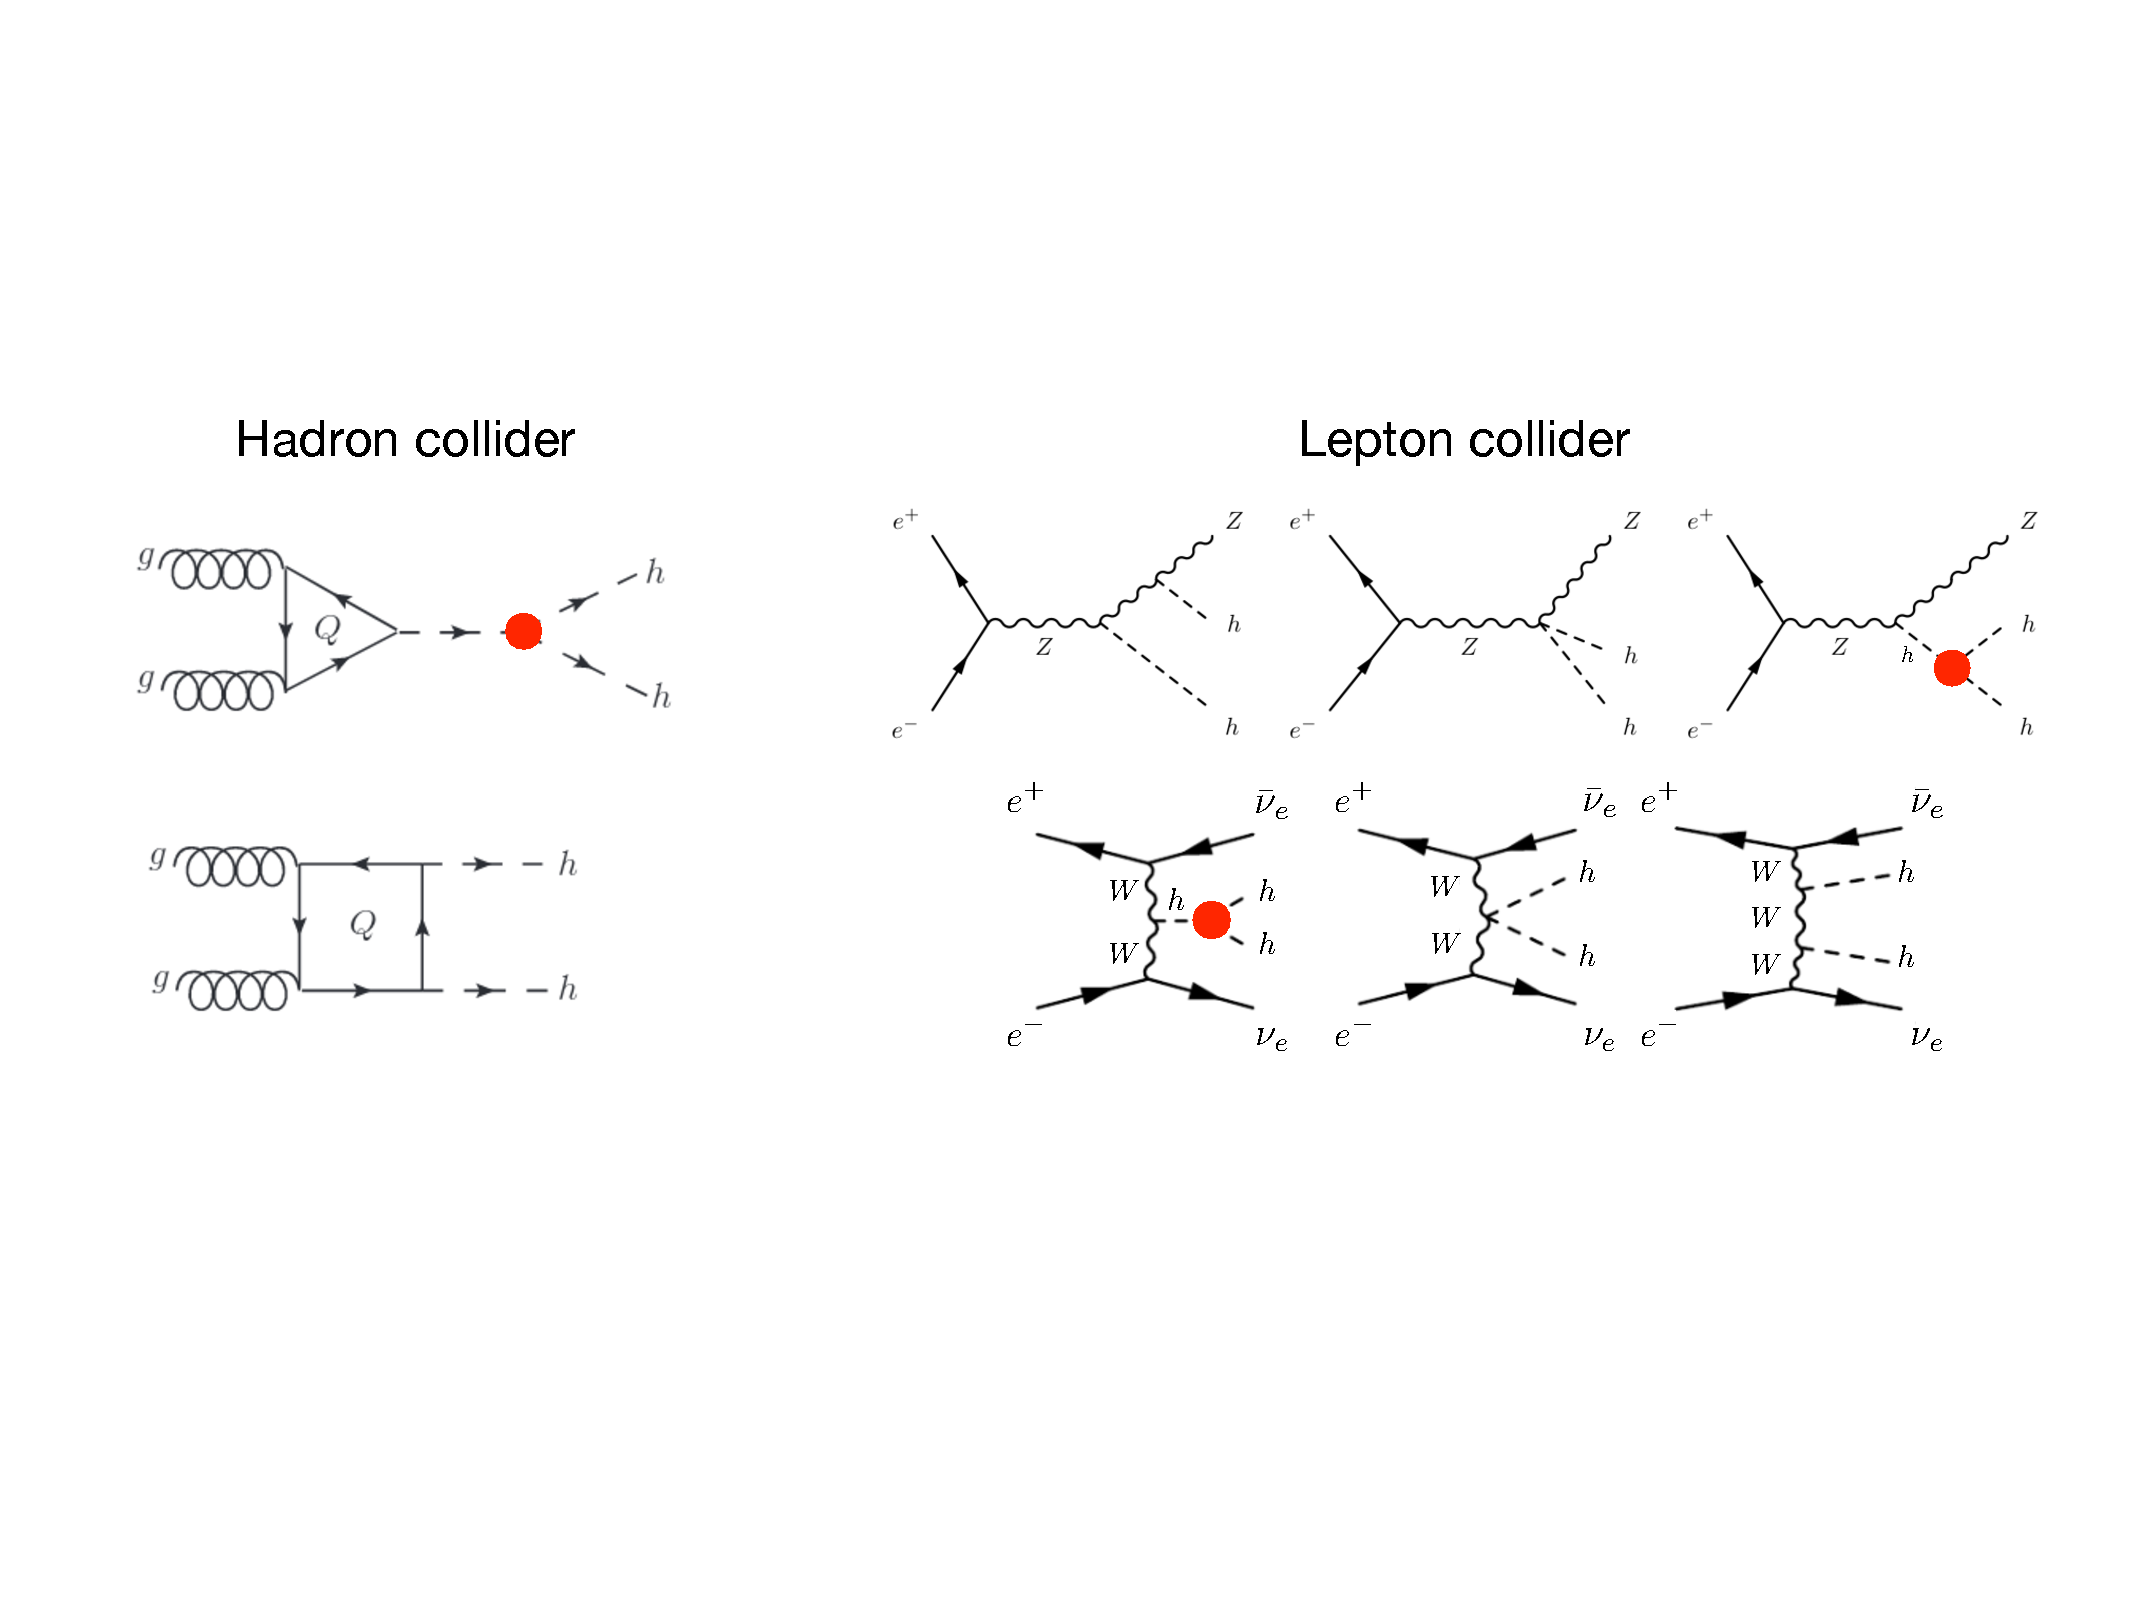
\includegraphics[width=0.80\textwidth]{Figs/Hself/HH-Feynman-all_v2.pdf}
  \caption{Representative diagrams contributing to Higgs pair production and the Higgs self-coupling programme. Source: Ref.~\cite{ECFAFactories2025}.}
  \label{fig:hh-diagrams}
\end{figure}
The key lesson is that a projection is meaningful only after the measured observable, the assumptions entering its extraction, and the dominant uncertainty sources have been identified.

Figure~\ref{fig:hh-cross-section} is used here as a visual anchor for the surrounding discussion. The important point is not only the numerical projection shown in the figure, but also the way in which the relevant FCC observable is connected to a physical parameter of the Standard Model or to a possible deviation from it.
\begin{figure}[H]
  \centering
  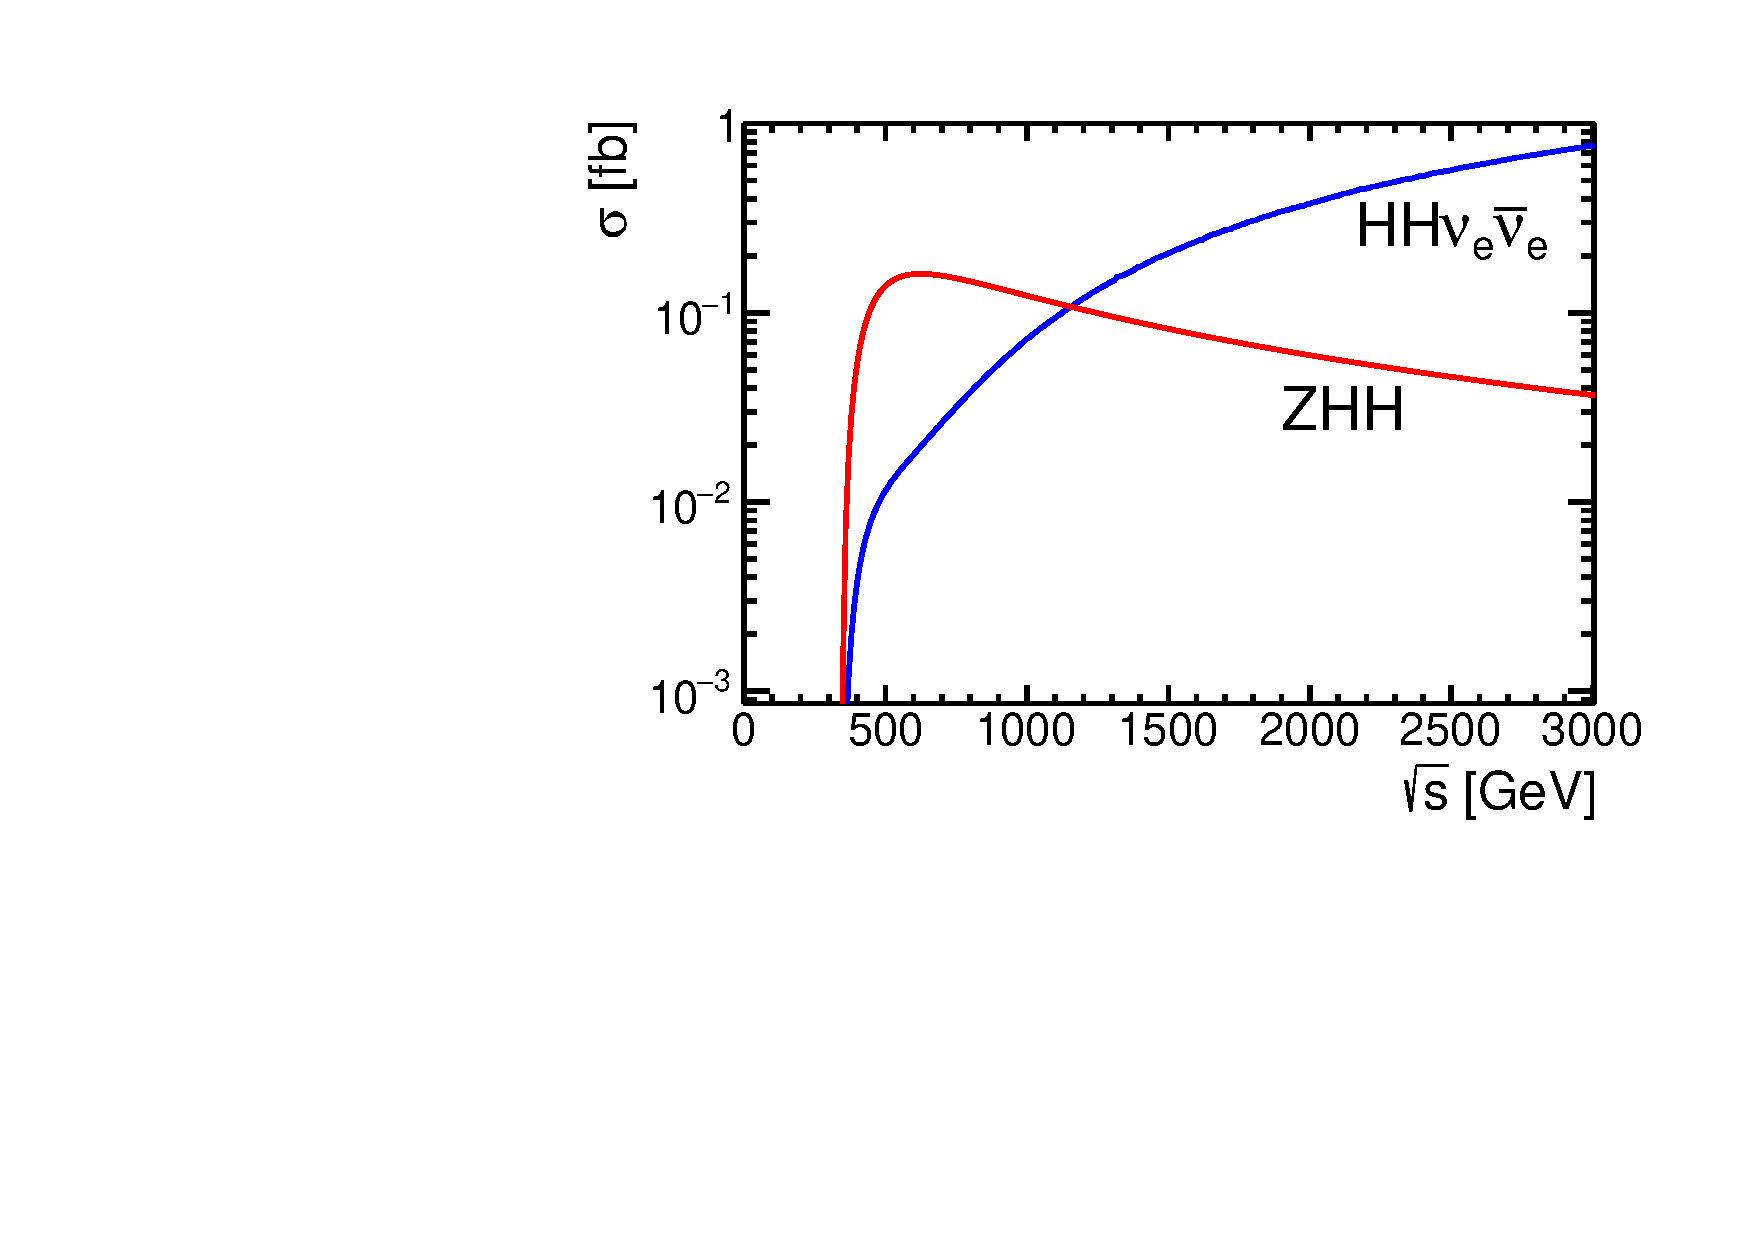
\includegraphics[width=0.85\textwidth]{Figs/Hself/CrossSectionPlot.pdf}
  \caption{Dependence of Higgs pair-production cross sections on the trilinear Higgs coupling at hadron and lepton colliders. Source: Ref.~\cite{ECFAFactories2025}.}
  \label{fig:hh-cross-section}
\end{figure}
The key lesson is that a projection is meaningful only after the measured observable, the assumptions entering its extraction, and the dominant uncertainty sources have been identified.

Figure~\ref{fig:kappalambda-fccee} is used here as a visual anchor for the surrounding discussion. The important point is not only the numerical projection shown in the figure, but also the way in which the relevant FCC observable is connected to a physical parameter of the Standard Model or to a possible deviation from it.
\begin{figure}[H]
  \centering
  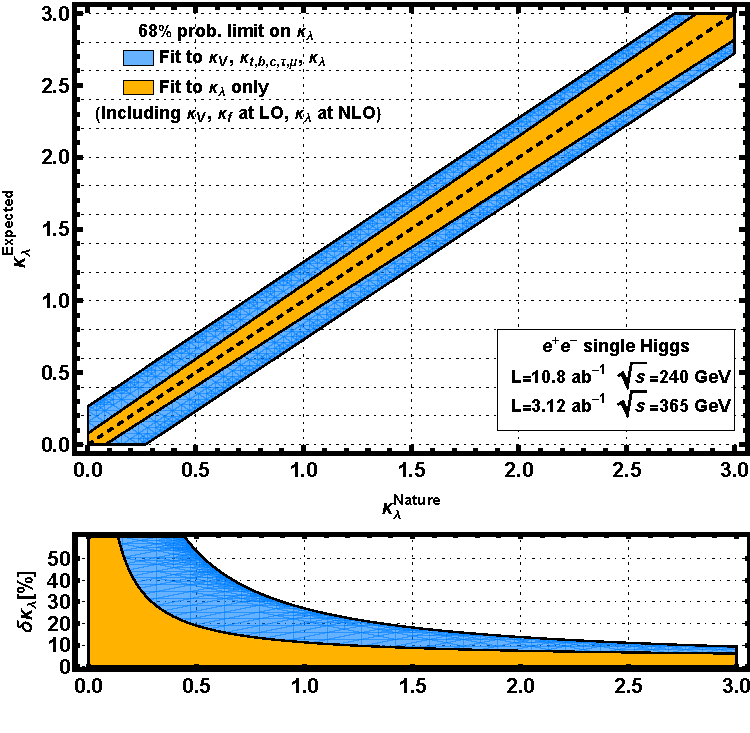
\includegraphics[width=0.80\textwidth]{Figs/Hself/KappaLambdaHEFT_FCCee.pdf}
  \caption{FCC-ee loop sensitivity to the Higgs self-coupling in effective-field-theory interpretations. Source: Ref.~\cite{MauraHiggsSelf2025}.}
  \label{fig:kappalambda-fccee}
\end{figure}
The key lesson is that a projection is meaningful only after the measured observable, the assumptions entering its extraction, and the dominant uncertainty sources have been identified.

Figure~\ref{fig:hhh-ecm} is used here as a visual anchor for the surrounding discussion. The important point is not only the numerical projection shown in the figure, but also the way in which the relevant FCC observable is connected to a physical parameter of the Standard Model or to a possible deviation from it.
\begin{figure}[H]
  \centering
  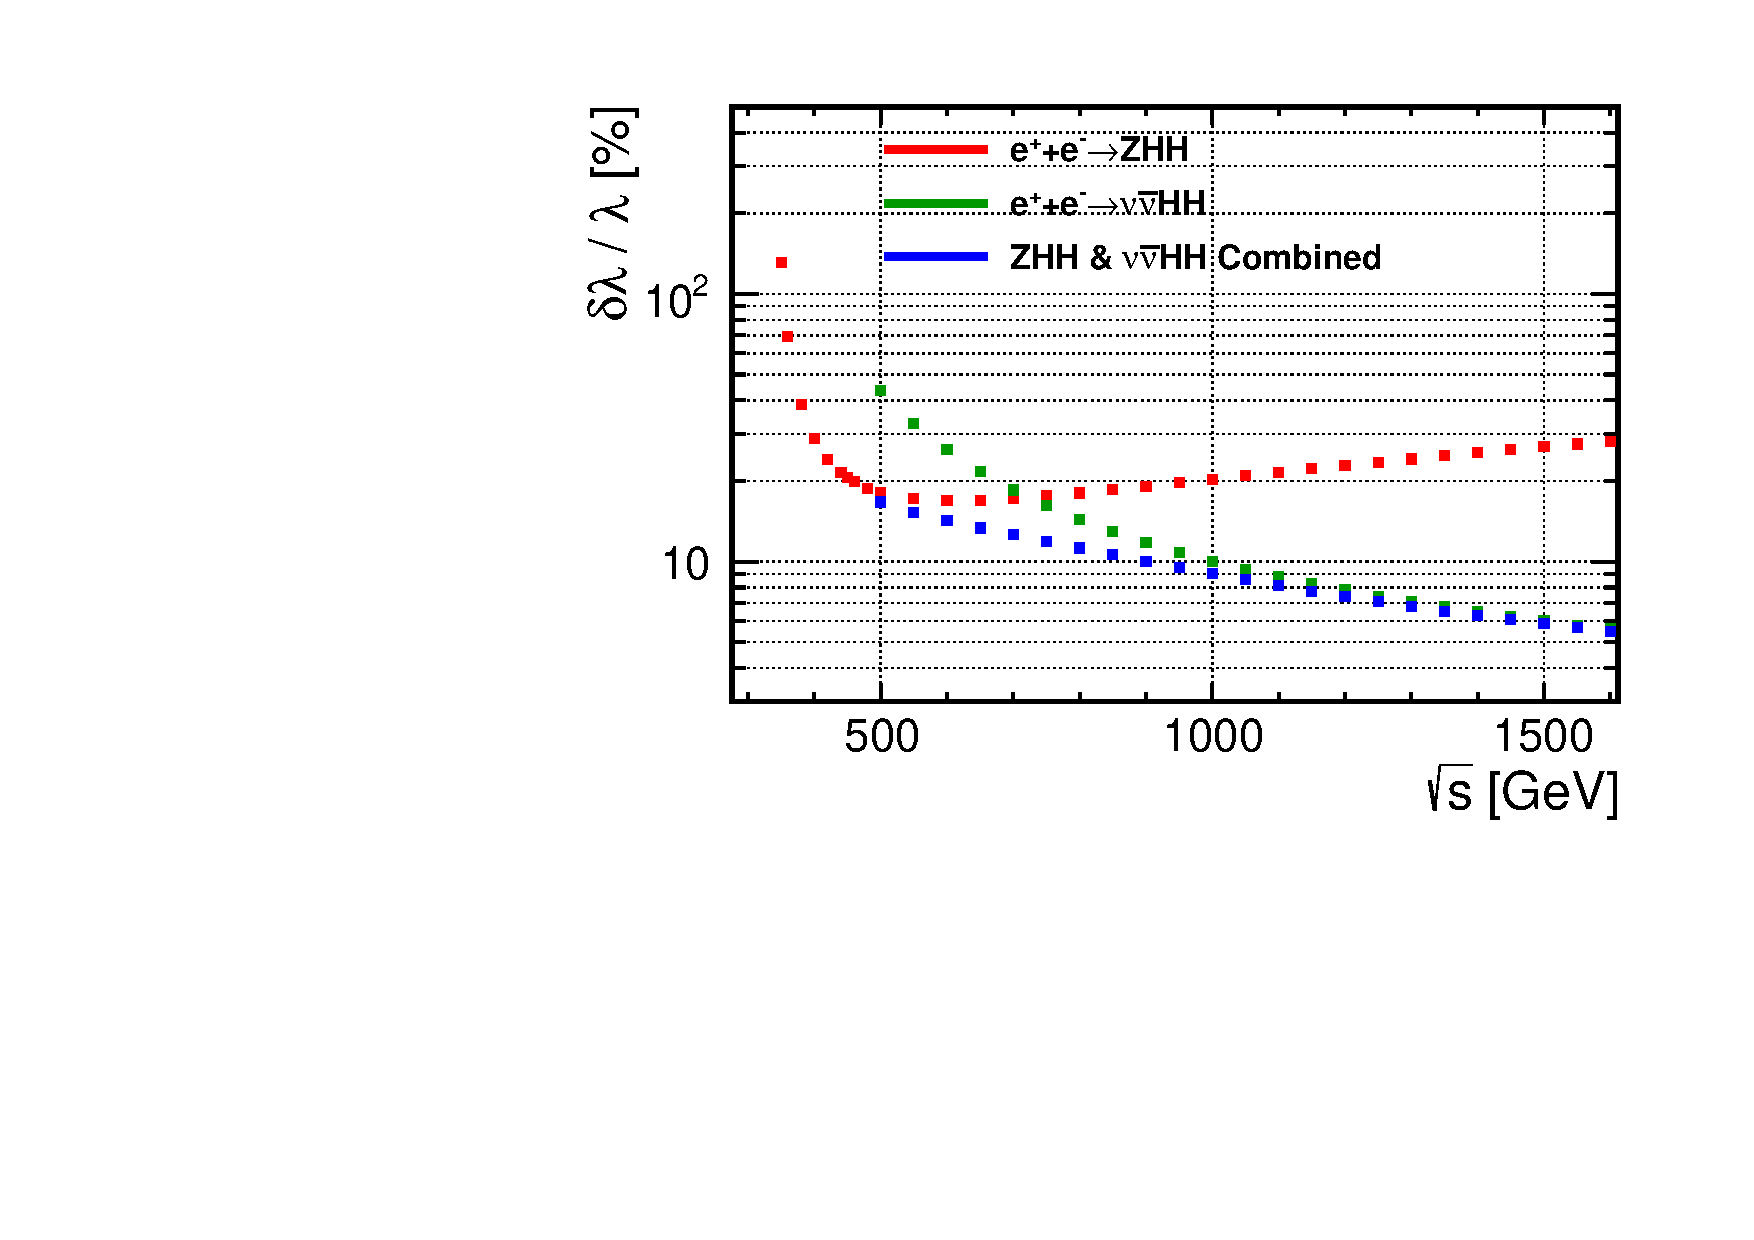
\includegraphics[width=0.82\textwidth]{Figs/Hself/HHH_ECM_Combined_new.pdf}
  \caption{Sensitivity to the Higgs self-coupling as a function of centre-of-mass energy and collider programme. Source: Ref.~\cite{ECFAFactories2025}.}
  \label{fig:hhh-ecm}
\end{figure}
The key lesson is that a projection is meaningful only after the measured observable, the assumptions entering its extraction, and the dominant uncertainty sources have been identified.

\begin{examplebox}{Extracting \(g_{Hbb}\) from Higgsstrahlung}{ghbb-example}
Suppose \(\sigma_{ZH}\) determines \(g_{HZZ}^2\), and the rate \(\sigma_{ZH}\BR(H\to b\bar b)\) is measured. Dividing the exclusive rate by the inclusive rate gives \(\BR(H\to b\bar b)\), but the partial width satisfies \(\Gamma_{bb}\propto g_{Hbb}^2\). Therefore \(g_{Hbb}\) requires either \(\Gamma_H\) or a global fit that determines \(\Gamma_H\) simultaneously. This is why the width extraction is a central part of the FCC-ee Higgs programme.
\end{examplebox}

\subsection{Exercises}
\begin{enumerate}[leftmargin=1.6em]
\item Derive Eq.~\eqref{eq:recoil-mass} and explain why the result is independent of the Higgs decay mode.
\item Starting from \(\mu_i^f=\kappa_i^2\kappa_f^2/\kappa_H^2\), show why a universal rescaling of all Higgs couplings can be difficult to determine without an absolute width constraint.
\item Explain qualitatively why \(\kappa_\lambda\) affects single-Higgs observables at loop level.
\item Write the list of detector capabilities required to separate \(H\to b\bar b\), \(H\to c\bar c\) and \(H\to gg\).
\end{enumerate}

\begin{takehomebox}
The recoil measurement is the conceptual cornerstone of FCC-ee Higgs physics. It changes Higgs measurements from relative rate comparisons into an absolute coupling and width programme.
\end{takehomebox}


\newpage
\section{Electroweak precision physics}
\begin{guidelinebox}
The electroweak programme is the precision backbone of FCC-ee, as emphasised in the FCC Feasibility Study and in dedicated Z-lineshape and W-threshold studies~\cite{FCCFSRVol1,ZLineshape2021,WMassWidth2021}. The Z pole supplies enormous statistics and exceptionally clean pseudo-observables, while the WW threshold determines the W mass and width. Together with the top and Higgs measurements, these observables form a high-precision closure test of the Standard Model.
\end{guidelinebox}

\subsection{Z-pole observables}
At the Z pole the basic process is
\begin{equation}
  e^+e^-\to Z\to f\bar f .
\end{equation}
The key pseudo-observables include
\begin{equation}
  \mZ,\quad \gZ,\quad \sigma^0_{\rm had},\quad R_\ell,\quad R_b,\quad R_c,\quad A_{\rm FB}^{0,f},\quad A_f,\quad \sin^2\theta_{\rm eff}^{\ell} .
\end{equation}
The hadronic pole cross section is
\begin{equation}
  \sigma^0_{\rm had}=\frac{12\pi}{m_Z^2}\frac{\Gamma_e\Gamma_{\rm had}}{\Gamma_Z^2} .
  \label{eq:sigma-had-pole}
\end{equation}
Ratios of partial widths are defined by
\begin{equation}
  R_\ell=\frac{\Gamma_{\rm had}}{\Gamma_{\ell\ell}},\qquad
  R_b=\frac{\Gamma_{b\bar b}}{\Gamma_{\rm had}},\qquad
  R_c=\frac{\Gamma_{c\bar c}}{\Gamma_{\rm had}} .
\end{equation}

Figure~\ref{fig:z-pole} is used here as a visual anchor for the surrounding discussion. The important point is not only the numerical projection shown in the figure, but also the way in which the relevant FCC observable is connected to a physical parameter of the Standard Model or to a possible deviation from it.
\begin{figure}[H]
  \centering
  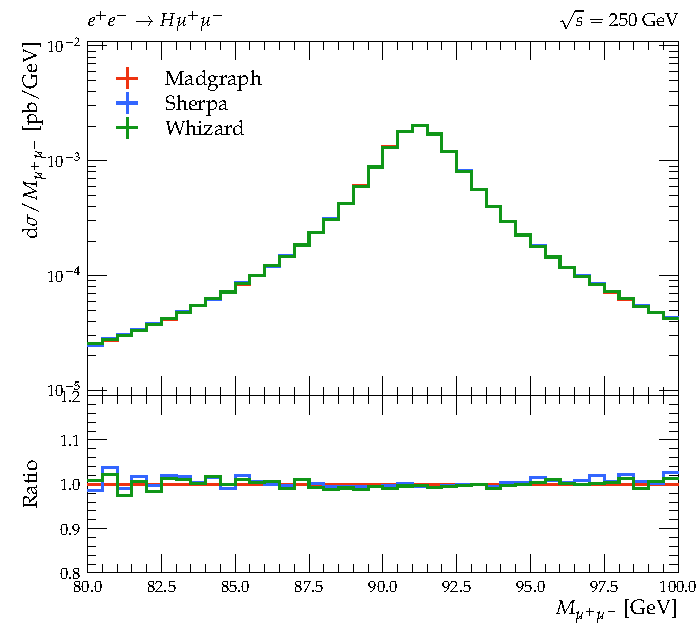
\includegraphics[width=0.80\textwidth]{Figs/commontools/Z_mass_pole.pdf}
  \caption{Illustration of the Z pole as a precision laboratory for mass, width, asymmetry and flavour observables. Source: Ref.~\cite{ECFAFactories2025}.}
  \label{fig:z-pole}
\end{figure}
The key lesson is that a projection is meaningful only after the measured observable, the assumptions entering its extraction, and the dominant uncertainty sources have been identified.

\begin{table}[H]
\centering
\small
\caption{Sample FCC-ee electroweak precision targets and theory requirements. The entries summarise representative values from the FCC Feasibility Study Report Vol.~1, Table~10; statistical and systematic components are quoted where the source separates them.}
\label{tab:ew-precision-benchmarks}
\begin{tabularx}{\textwidth}{@{}p{2.3cm}p{2.25cm}p{2.7cm}X@{}}
\toprule
Quantity & Current precision & FCC-ee projected precision & Main theory input \\
\midrule
\(m_Z\) & \(2.0\,\mathrm{MeV}\) & \(0.004\,(0.1)\,\mathrm{MeV}\) & Lineshape modelling, non-resonant \(e^+e^-\to f\bar f\), ISR and NNLO corrections.\\
\(\Gamma_Z\) & \(2.3\,\mathrm{MeV}\) & \(0.004\,(0.012)\,\mathrm{MeV}\) & Z-pole lineshape theory and radiative corrections.\\
\(\sin^2\theta_{\rm eff}^{\ell}\) & \(1.6\times10^{-4}\) & \(1.2(1.2)\times10^{-6}\) & Higher-order electroweak vertex corrections and input-parameter control.\\
\(m_W\) & \(9.9\,\mathrm{MeV}\) & \(0.18\,(0.16)\,\mathrm{MeV}\) & \(e^+e^-\to WW\) threshold lineshape, EFT setup and NNLO calculations.\\
\(HZZ\) coupling & -- & \(0.1\%\) & Precision \(e^+e^-\to ZH\) cross-section theory.\\
\(m_t\) & \(290\,\mathrm{MeV}\) & \(4.2(4.9)\,\mathrm{MeV}\) experimental components & \(t\bar t\) threshold theory, matching, resummation and \(\alpha_s\) input.\\
\bottomrule
\end{tabularx}
\end{table}
These targets are so precise that the limiting uncertainty can move from data statistics to theory and calibration. This is why electroweak physics at FCC-ee is inseparable from beam-energy calibration, luminosity theory and multi-loop calculations.

\begin{definition}{Electroweak pseudo-observable}{ewpo}
An electroweak pseudo-observable is a quantity extracted from measured cross sections and asymmetries after unfolding well-defined QED and experimental effects, so that it can be compared to Standard Model predictions in a convention-independent way. Examples include \(\mZ\), \(\gZ\), \(\sigma^0_{\rm had}\), \(R_b\), and \(A_{\rm FB}^{0,f}\).
\end{definition}

\subsection{Asymmetries and effective weak mixing angle}
The vector and axial couplings of the Z boson to a fermion \(f\) can be written as
\begin{equation}
  g_A^f=T_3^f,\qquad
  g_V^f=T_3^f-2Q_f\sin^2\theta_{\rm eff}^f .
\end{equation}
The asymmetry parameter is
\begin{equation}
  A_f=\frac{2g_V^fg_A^f}{(g_V^f)^2+(g_A^f)^2},
\end{equation}
and the pole forward-backward asymmetry is
\begin{equation}
  A_{\rm FB}^{0,f}=\frac34 A_eA_f .
  \label{eq:afb}
\end{equation}
Because \(g_V^\ell\) is numerically small for charged leptons, leptonic asymmetries are extremely sensitive to \(\sin^2\theta_{\rm eff}^\ell\). This is why the Tera-Z programme is a powerful electroweak microscope.

Figure~\ref{fig:mw-mt-plane} is used here as a visual anchor for the surrounding discussion. The important point is not only the numerical projection shown in the figure, but also the way in which the relevant FCC observable is connected to a physical parameter of the Standard Model or to a possible deviation from it.
\begin{figure}[H]
  \centering
  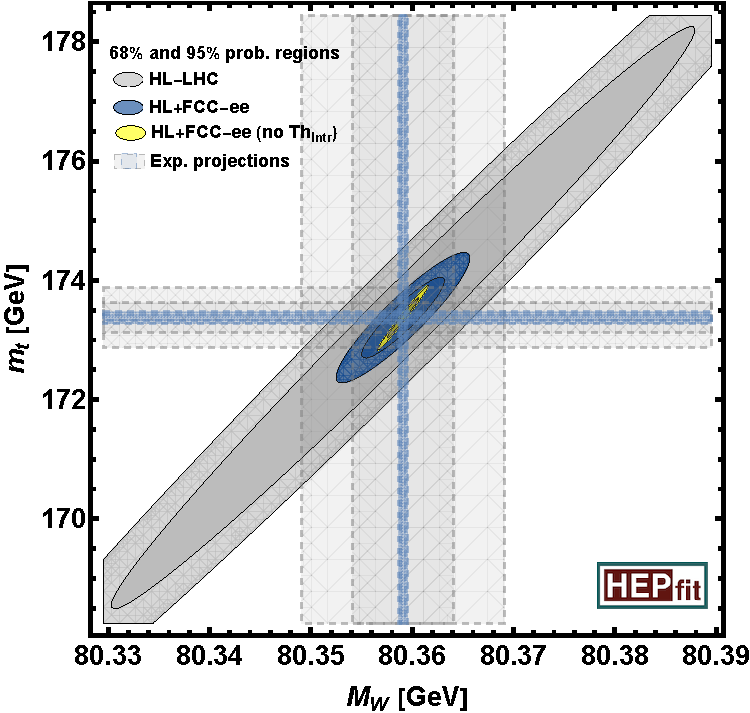
\includegraphics[width=0.80\textwidth]{Figs/EWfit/MWmtplot_FCCee.pdf}
  \caption{Electroweak closure test in the \((m_W,m_t)\) plane, illustrating how direct measurements and indirect fits sharpen consistency tests of the Standard Model. Source: Ref.~\cite{DefranchisTopThreshold2025}.}
  \label{fig:mw-mt-plane}
\end{figure}
The key lesson is that a projection is meaningful only after the measured observable, the assumptions entering its extraction, and the dominant uncertainty sources have been identified.

Figure~\ref{fig:mt-mw-uncert} is used here as a visual anchor for the surrounding discussion. The important point is not only the numerical projection shown in the figure, but also the way in which the relevant FCC observable is connected to a physical parameter of the Standard Model or to a possible deviation from it.
\begin{figure}[H]
  \centering
  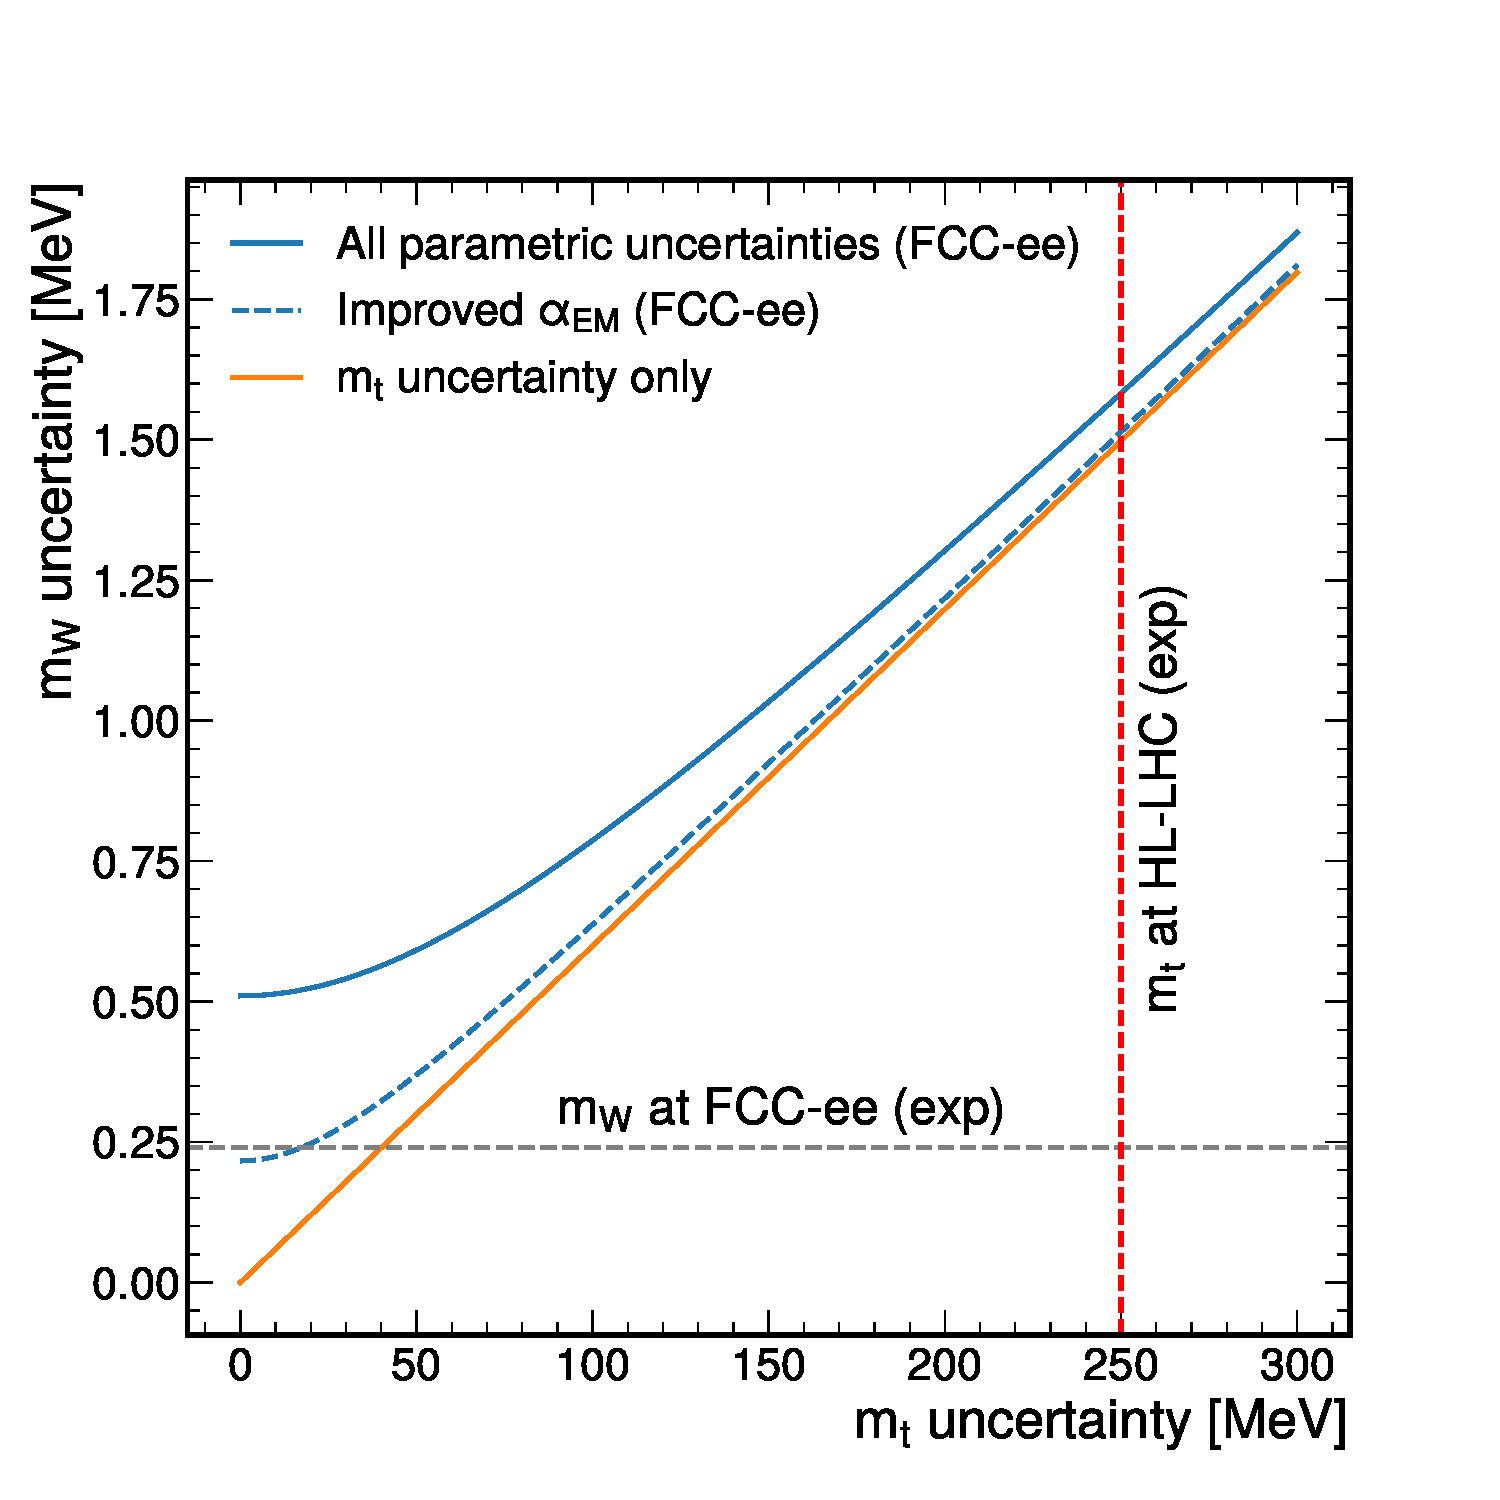
\includegraphics[width=0.78\textwidth]{Figs/EWfit/mt_mW_uncert.pdf}
  \caption{Impact of top-mass precision on the Standard Model prediction for the W mass. Source: Ref.~\cite{DefranchisTopThreshold2025}.}
  \label{fig:mt-mw-uncert}
\end{figure}
The key lesson is that a projection is meaningful only after the measured observable, the assumptions entering its extraction, and the dominant uncertainty sources have been identified.

\subsection{WW threshold}
Near threshold, the cross section
\begin{equation}
  e^+e^-\to W^+W^-\to 4f
\end{equation}
changes rapidly with the W mass. A threshold scan therefore determines \(\mW\) from the energy dependence of \(\sigma_{WW}\), and \(\gW\) from the shape and normalisation. The relevant observables include
\begin{equation}
  \mW,\qquad \gW,\qquad \BR(W\to \ell\nu),\qquad \BR(W\to q\bar q') .
\end{equation}
The WW threshold is also sensitive to triple gauge couplings and to electroweak corrections that must be controlled at the level implied by the projected experimental uncertainty.

Figure~\ref{fig:mwmt-new} is used here as a visual anchor for the surrounding discussion. The important point is not only the numerical projection shown in the figure, but also the way in which the relevant FCC observable is connected to a physical parameter of the Standard Model or to a possible deviation from it.
\begin{figure}[H]
  \centering
  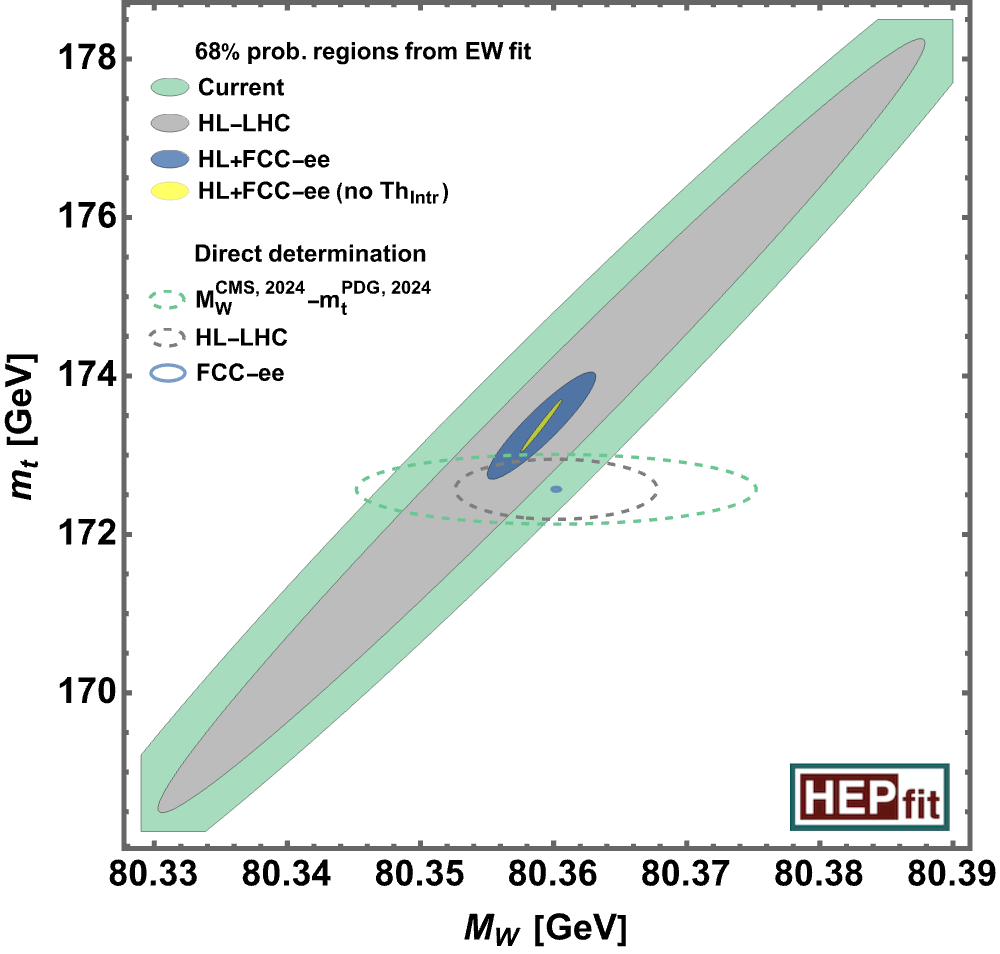
\includegraphics[width=0.80\textwidth]{Figs/MWmtplot_FCCee_New.png}
  \caption{Projected FCC-ee improvement in the electroweak-fit closure relation between \(m_W\) and \(m_t\). Source: Ref.~\cite{FCCManifesto2025}.}
  \label{fig:mwmt-new}
\end{figure}
The key lesson is that a projection is meaningful only after the measured observable, the assumptions entering its extraction, and the dominant uncertainty sources have been identified.

\subsection{Beam-energy calibration and resonant depolarisation}
Electroweak precision at FCC-ee depends critically on knowing the centre-of-mass energy. Resonant depolarisation provides a unique calibration handle at circular lepton colliders. If the beam energy is shifted by an amount comparable to or larger than the target uncertainty on \(\mZ\) or \(\mW\), the measurement becomes systematics limited even with enormous statistics. This is why accelerator physics and precision phenomenology are tightly coupled in the FCC-ee programme.

\begin{remarkbox}{Statistics are not the main difficulty}{statistics-ew}
At the Z pole, the number of events is so large that statistical uncertainty is often not the limiting challenge. The limiting issues become beam energy, luminosity, acceptance, flavour tagging, QED radiation, electroweak higher orders and correlations among experiments.
\end{remarkbox}

Figure~\ref{fig:w-effective-couplings} is used here as a visual anchor for the surrounding discussion. The important point is not only the numerical projection shown in the figure, but also the way in which the relevant FCC observable is connected to a physical parameter of the Standard Model or to a possible deviation from it.
\begin{figure}[H]
  \centering
  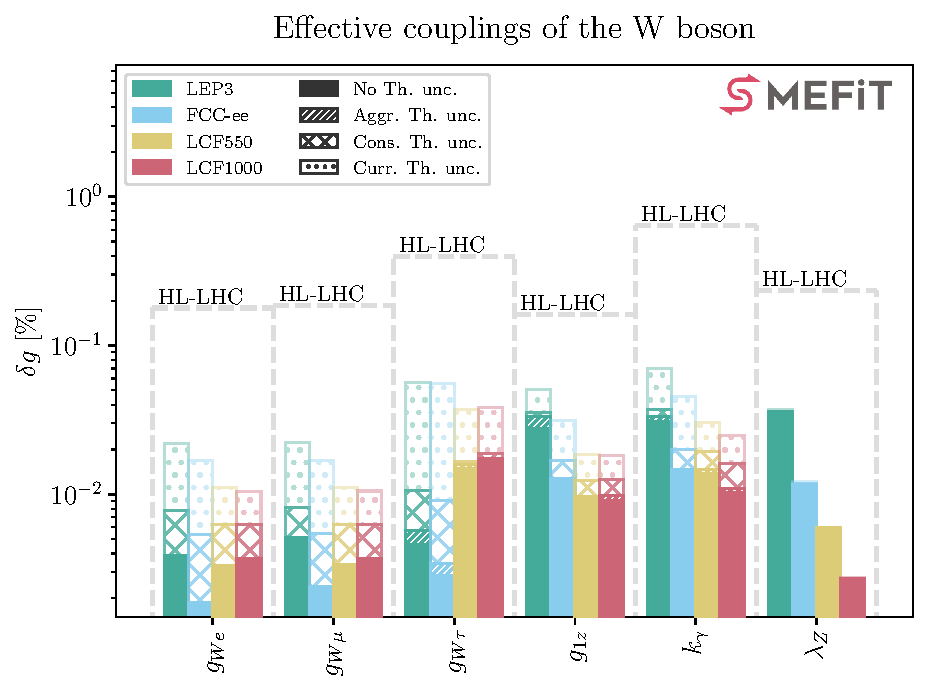
\includegraphics[width=0.78\textwidth]{Figs/Effective_couplings_of_the_W_boson.pdf}
  \caption{Projected constraints on effective W-boson couplings in future collider fits. Source: Ref.~\cite{ArmadilloSMEFiT2026}.}
  \label{fig:w-effective-couplings}
\end{figure}
The key lesson is that a projection is meaningful only after the measured observable, the assumptions entering its extraction, and the dominant uncertainty sources have been identified.

Figure~\ref{fig:left-ew-couplings} is used here as a visual anchor for the surrounding discussion. The important point is not only the numerical projection shown in the figure, but also the way in which the relevant FCC observable is connected to a physical parameter of the Standard Model or to a possible deviation from it.
\begin{figure}[H]
  \centering
  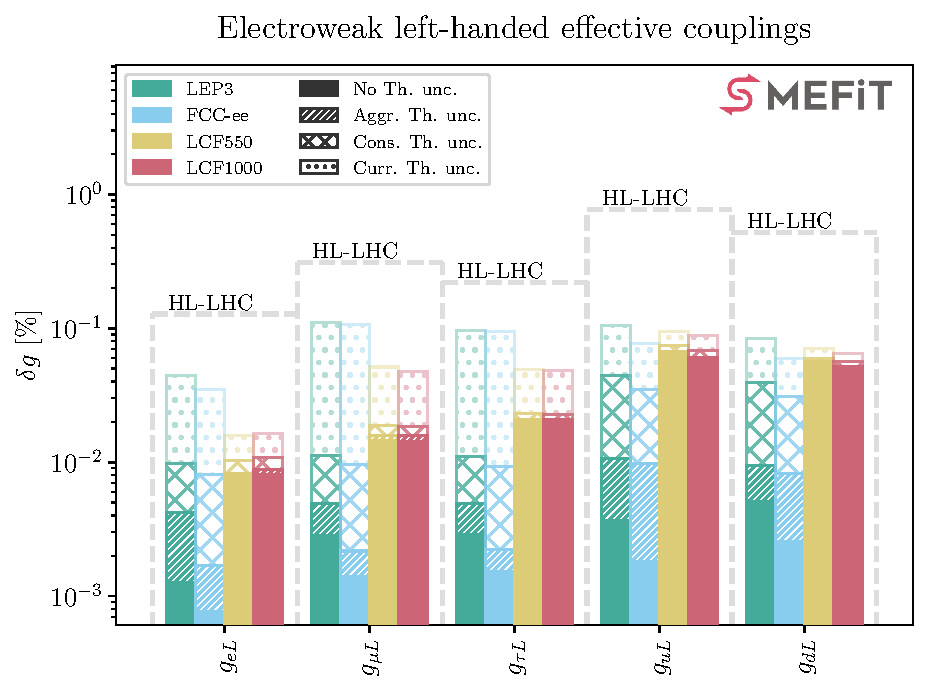
\includegraphics[width=0.78\textwidth]{Figs/Electroweak_left-handed_effective_couplings.pdf}
  \caption{Projected constraints on left-handed electroweak effective couplings. Source: Ref.~\cite{ArmadilloSMEFiT2026}.}
  \label{fig:left-ew-couplings}
\end{figure}
The key lesson is that a projection is meaningful only after the measured observable, the assumptions entering its extraction, and the dominant uncertainty sources have been identified.

Figure~\ref{fig:right-ew-couplings} is used here as a visual anchor for the surrounding discussion. The important point is not only the numerical projection shown in the figure, but also the way in which the relevant FCC observable is connected to a physical parameter of the Standard Model or to a possible deviation from it.
\begin{figure}[H]
  \centering
  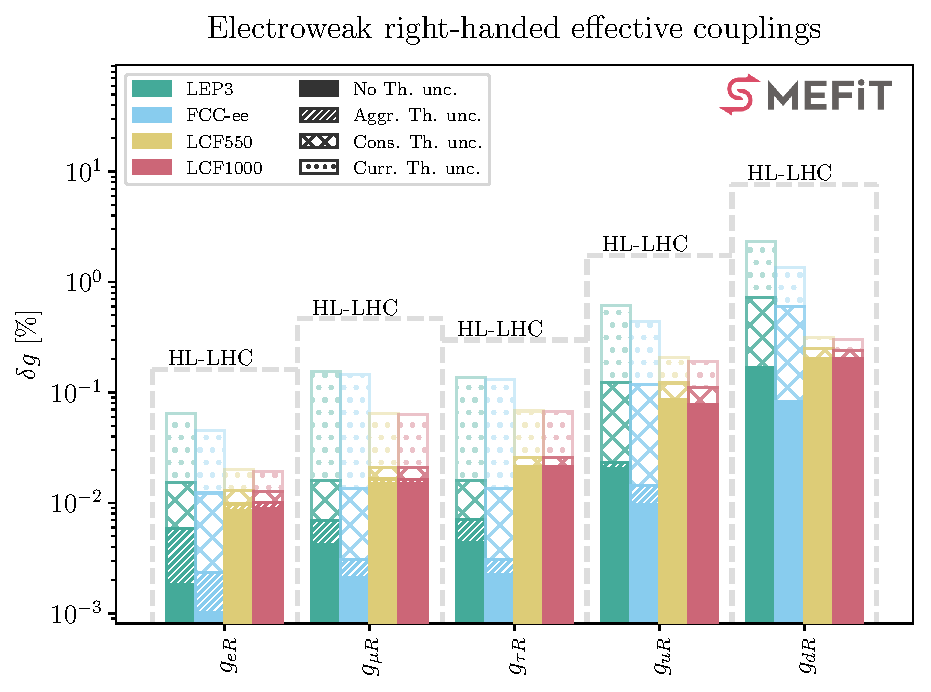
\includegraphics[width=0.78\textwidth]{Figs/Electroweak_right-handed_effective_couplings.pdf}
  \caption{Projected constraints on right-handed electroweak effective couplings. Source: Ref.~\cite{ArmadilloSMEFiT2026}.}
  \label{fig:right-ew-couplings}
\end{figure}
The key lesson is that a projection is meaningful only after the measured observable, the assumptions entering its extraction, and the dominant uncertainty sources have been identified.

For every precision observable it is useful to separate the total error into conceptually distinct pieces,
\begin{equation}
  \delta_{\rm tot}^2 = \delta_{\rm stat}^2 + \delta_{\rm exp\,syst}^2
  + \delta_{\rm th}^2 + \delta_{\rm param}^2 + \delta_{\rm model}^2 .
\end{equation}
The last term is not always quoted explicitly, but it is often the most subtle one: it includes choices of event generator, hadronisation model, flavour-tagging calibration, fit parametrisation, and assumptions used to project detector performance. A lecture-note treatment should therefore avoid saying that an uncertainty is ``small'' without stating relative to which component of the analysis.

\begin{examplebox}{Sensitivity of an asymmetry to \(\sin^2\theta_{\rm eff}\)}{asymmetry-example}
For a charged lepton, \(T_3=-1/2\) and \(Q=-1\), so \(g_V=-1/2+2\sin^2\theta_{\rm eff}\). Since \(\sin^2\theta_{\rm eff}\simeq0.23\), the vector coupling is small. A small change in \(\sin^2\theta_{\rm eff}\) therefore produces a relatively large fractional change in \(g_V/g_A\), which explains the power of asymmetry measurements.
\end{examplebox}

\begin{guidedchecksbox}
\begin{enumerate}[leftmargin=1.6em]
\item Derive Eq.~\eqref{eq:afb} from the angular distribution of \(e^+e^-\to Z\to f\bar f\).
\item Explain why \(\sigma^0_{\rm had}\) depends on \(\Gamma_Z^{-2}\).
\item Identify which uncertainty sources are experimental and which are theoretical in a W-threshold scan.
\end{enumerate}
\end{guidedchecksbox}

\subsection{Exercises}
\begin{enumerate}[leftmargin=1.6em]
\item Starting from the Z couplings, compute \(g_V^e\) and \(g_A^e\) for \(\sin^2\theta_{\rm eff}=0.231\).
\item Explain why the W mass, top mass and Higgs mass enter electroweak closure tests.
\item Discuss why a direct measurement of \(\alpha_{\rm QED}(m_Z^2)\) would reduce parametric uncertainties in the electroweak fit.
\end{enumerate}


\newpage
\section{Top-quark precision physics}
\begin{guidelinebox}
The top-quark threshold scan is one of the cleanest methods for measuring the top mass in a well-defined short-distance scheme. It is also a precision bridge between QCD, electroweak physics and Higgs physics, because the threshold line shape depends on \(m_t\), \(\Gamma_t\), \(\alpha_s\) and the top Yukawa coupling.
\end{guidelinebox}

\subsection{Processes and observables}
The idealised process is
\begin{equation}
  e^+e^-\to t\bar t,
\end{equation}
but the experimentally relevant final state is
\begin{equation}
  e^+e^-\to W^+bW^-\bar b .
\end{equation}
Near threshold, the cross section is a function of several parameters,
\begin{equation}
  \sigma_{WbWb}=\sigma_{WbWb}\left(\sqrt{s};m_t,\Gamma_t,\alpha_s,y_t,\ldots\right) .
  \label{eq:top-threshold-cross-section}
\end{equation}
The line shape shifts with \(m_t\), broadens with \(\Gamma_t\), and changes normalisation and shape with \(\alpha_s\) and \(y_t\). This is why the threshold scan is both powerful and theory demanding.

Figure~\ref{fig:top-threshold-ps} is used here as a visual anchor for the surrounding discussion. The important point is not only the numerical projection shown in the figure, but also the way in which the relevant FCC observable is connected to a physical parameter of the Standard Model or to a possible deviation from it.
\begin{figure}[H]
  \centering
  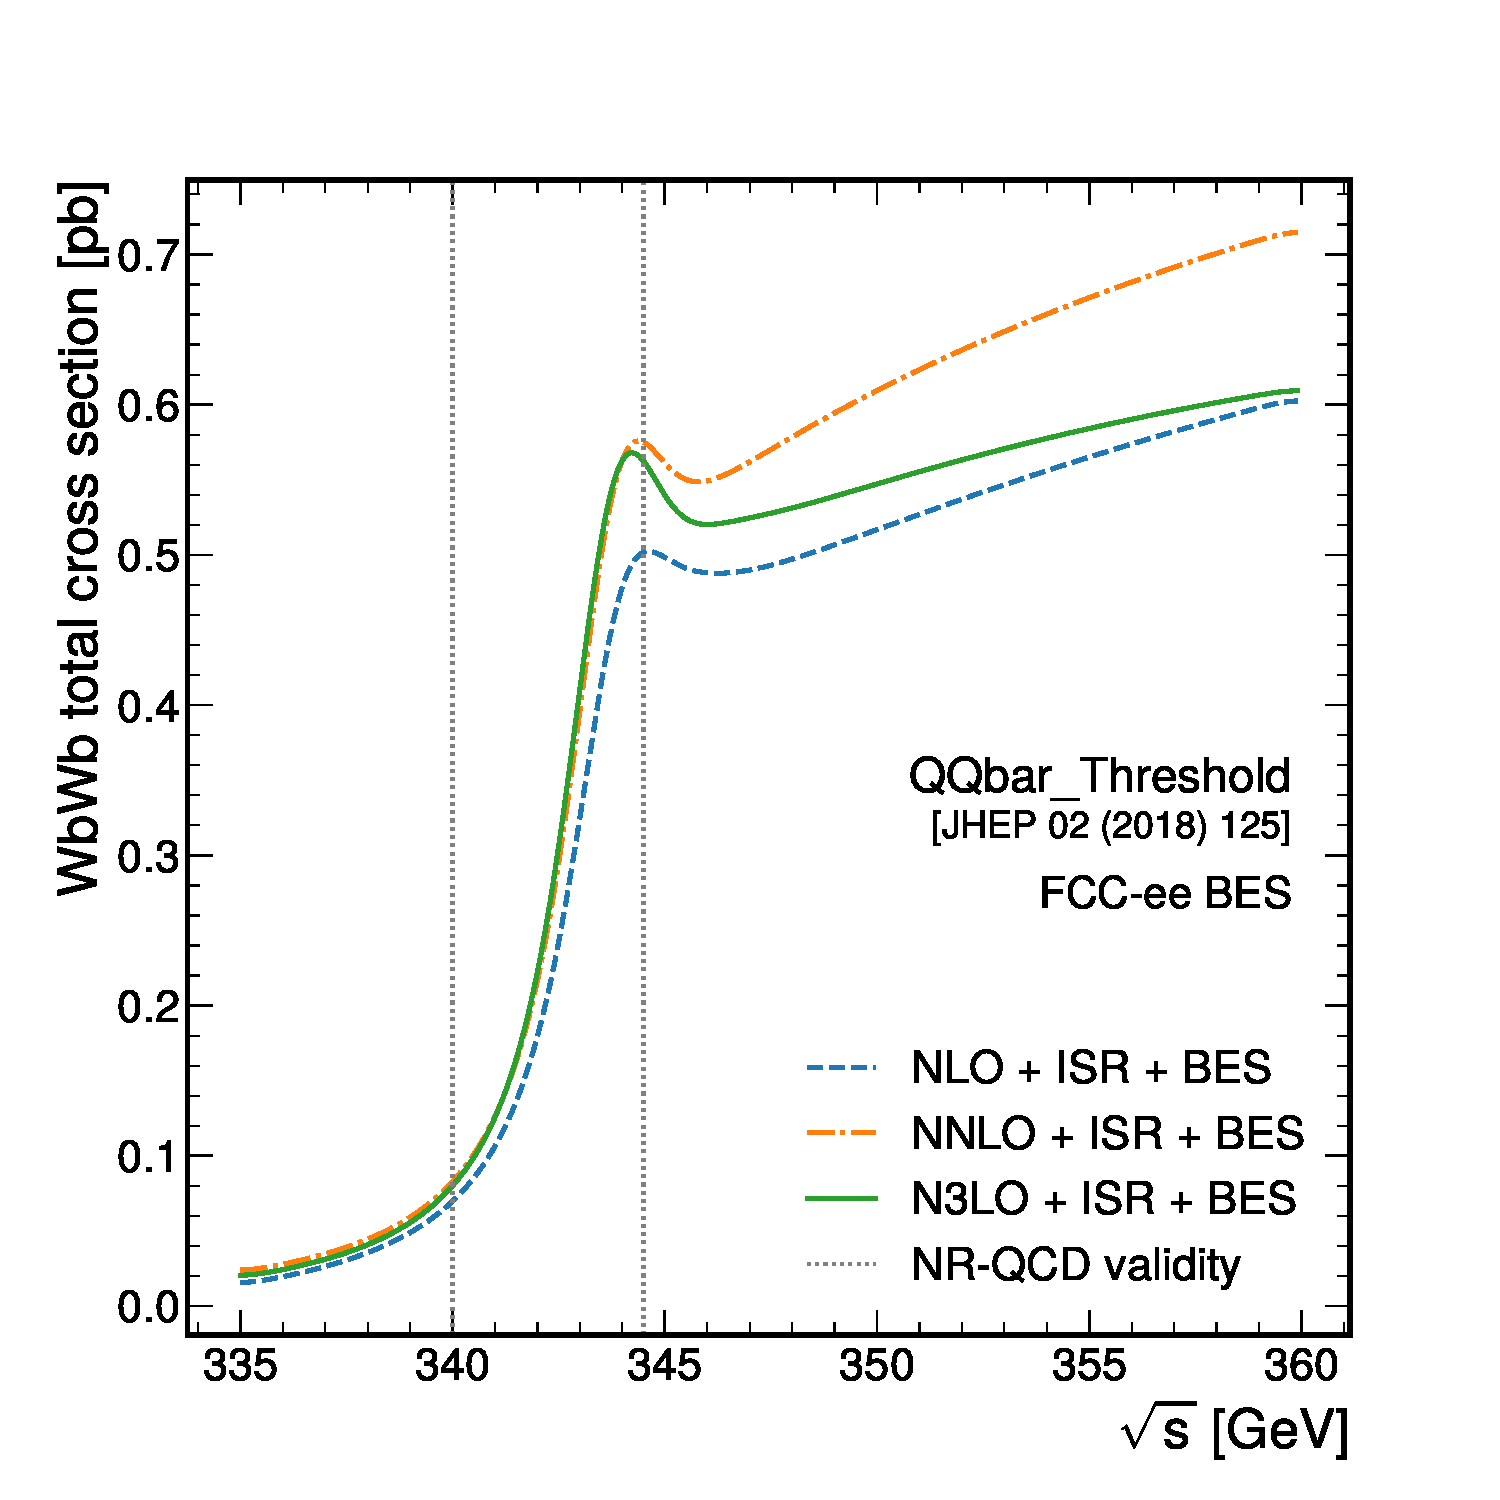
\includegraphics[width=0.85\textwidth]{Figs/scan/plot_PS.pdf}
  \caption{N3LO threshold prediction for \(e^+e^-\to W^+bW^-\bar b\), including effects relevant for the FCC-ee top threshold scan. Source: Ref.~\cite{DefranchisTopThreshold2025}.}
  \label{fig:top-threshold-ps}
\end{figure}
The key lesson is that a projection is meaningful only after the measured observable, the assumptions entering its extraction, and the dominant uncertainty sources have been identified.

Figure~\ref{fig:top-isr-bes} is used here as a visual anchor for the surrounding discussion. The important point is not only the numerical projection shown in the figure, but also the way in which the relevant FCC observable is connected to a physical parameter of the Standard Model or to a possible deviation from it.
\begin{figure}[H]
  \centering
  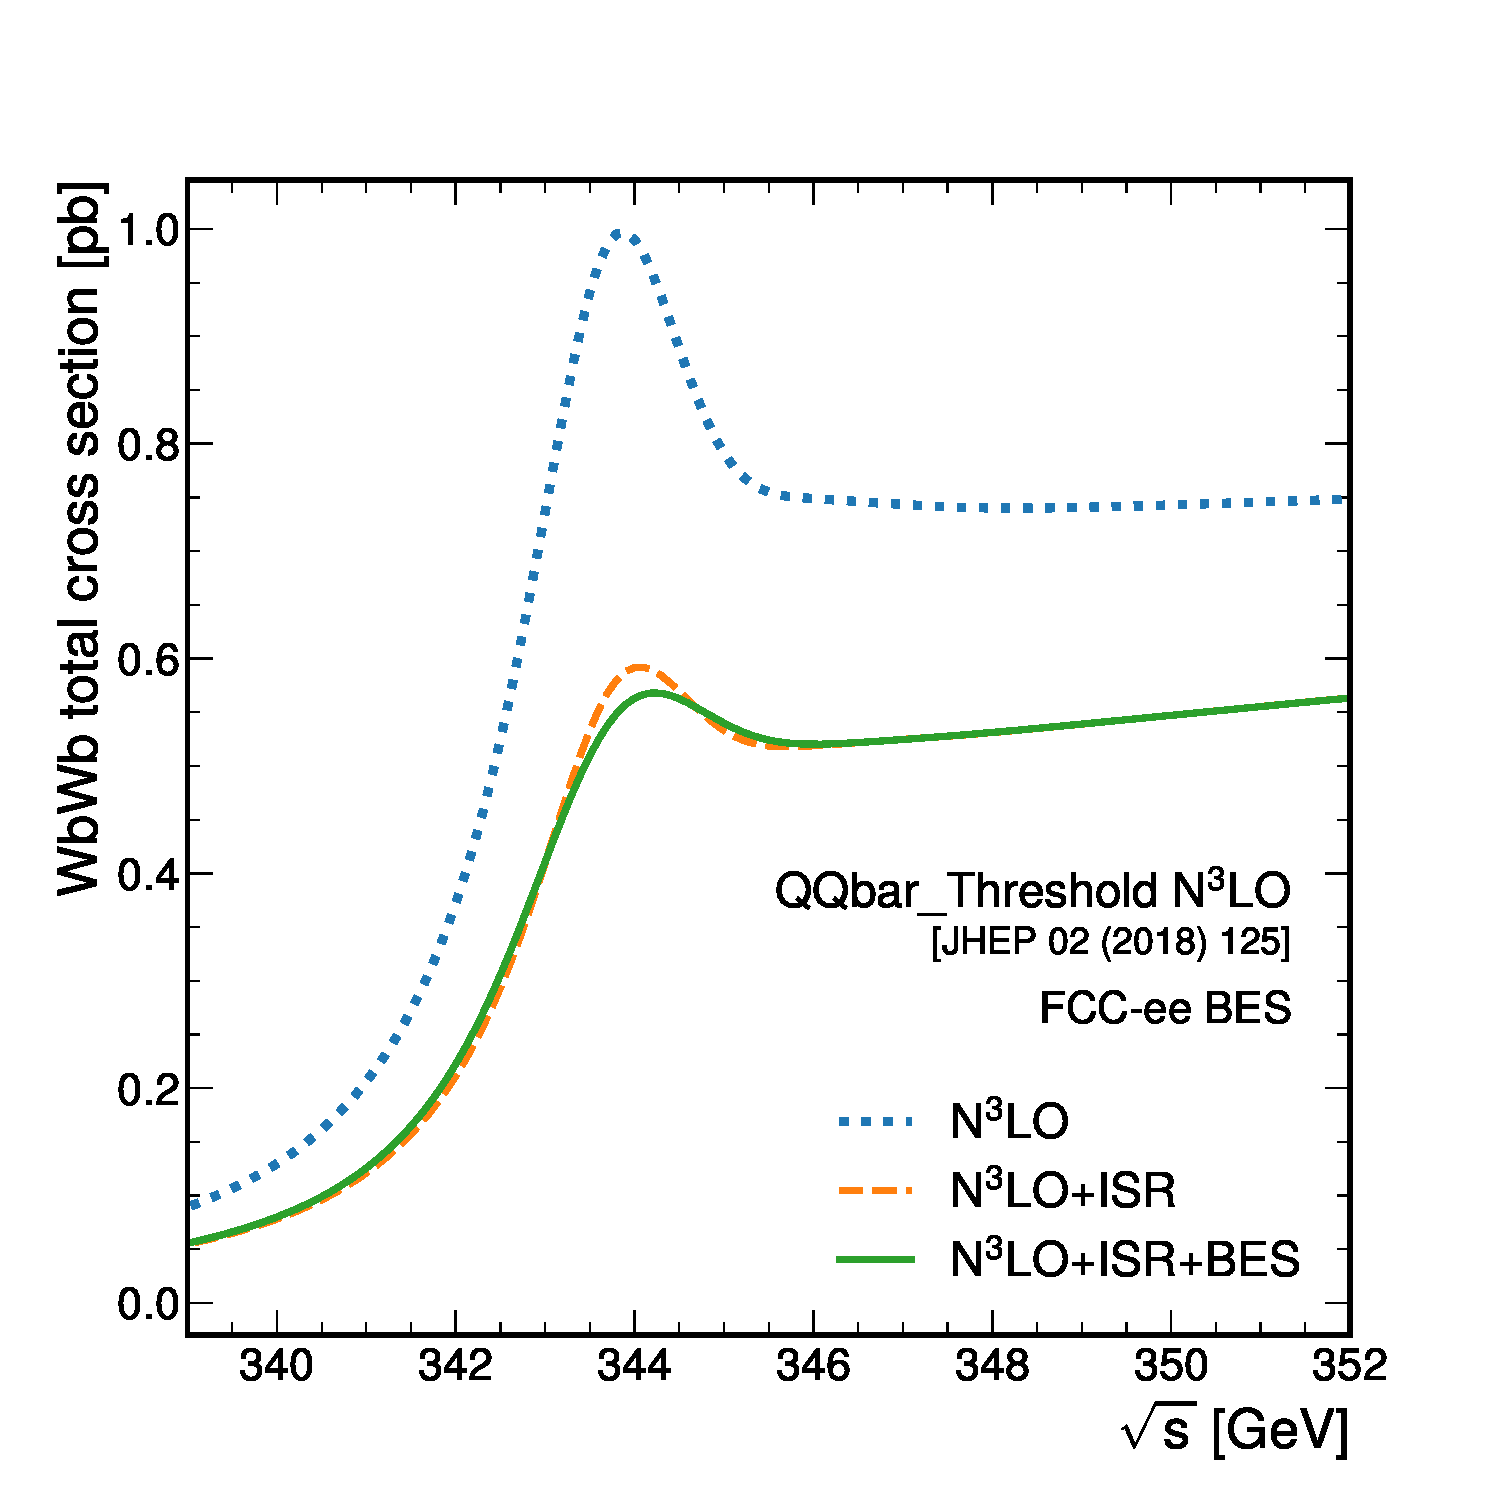
\includegraphics[width=0.85\textwidth]{Figs/scan/ISR_comparison_N3LO.pdf}
  \caption{Effect of initial-state radiation and beam-energy spread on the top-threshold line shape. Source: Ref.~\cite{DefranchisTopThreshold2025}.}
  \label{fig:top-isr-bes}
\end{figure}
The key lesson is that a projection is meaningful only after the measured observable, the assumptions entering its extraction, and the dominant uncertainty sources have been identified.

Figure~\ref{fig:top-param-dependence} is used here as a visual anchor for the surrounding discussion. The important point is not only the numerical projection shown in the figure, but also the way in which the relevant FCC observable is connected to a physical parameter of the Standard Model or to a possible deviation from it.
\begin{figure}[H]
  \centering
  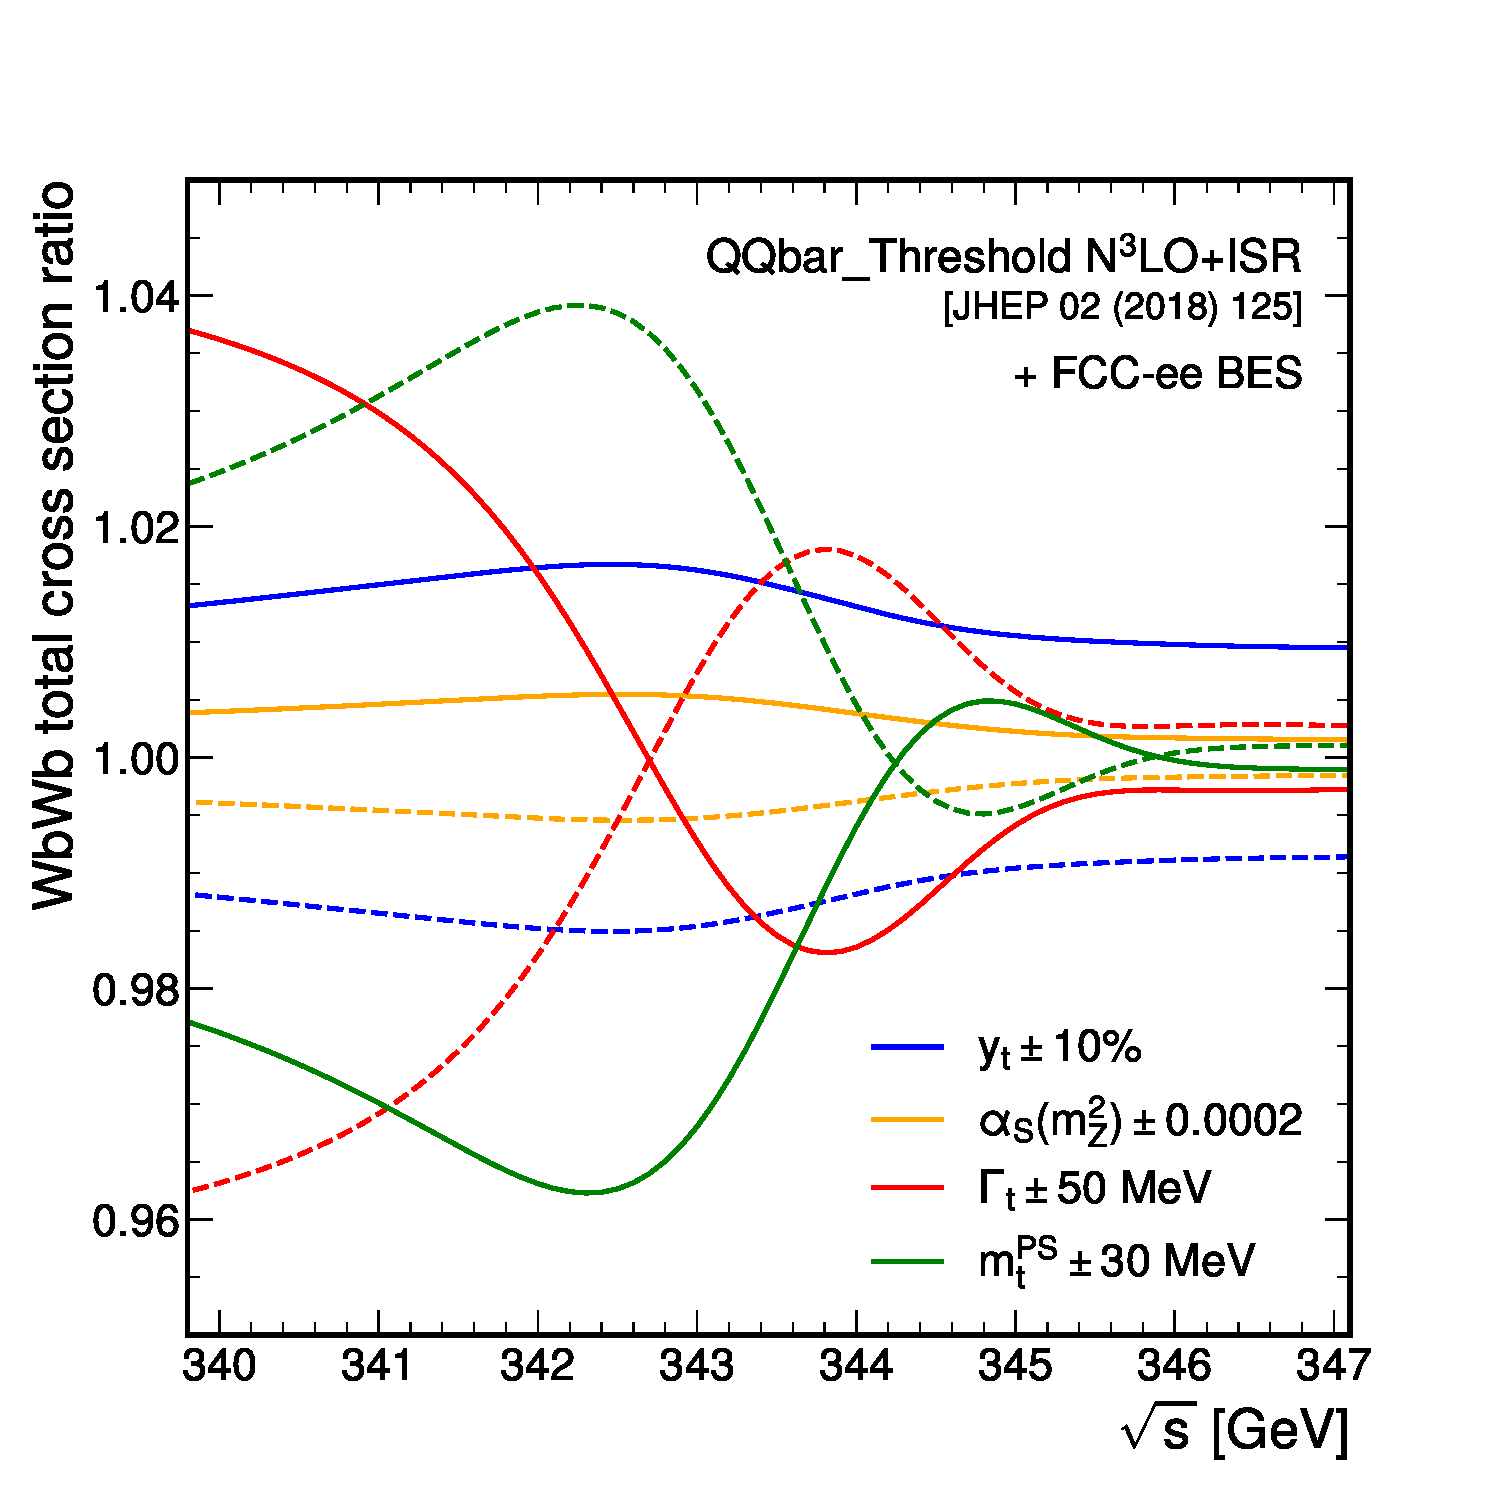
\includegraphics[width=0.85\textwidth]{Figs/scan/plot_N3LO_PS_yukawa_alphaS_ratio.pdf}
  \caption{Relative dependence of the threshold line shape on \(m_t\), \(\Gamma_t\), \(\alpha_s\) and the top Yukawa coupling. Source: Ref.~\cite{DefranchisTopThreshold2025}.}
  \label{fig:top-param-dependence}
\end{figure}
The key lesson is that a projection is meaningful only after the measured observable, the assumptions entering its extraction, and the dominant uncertainty sources have been identified.

\begin{definition}{Threshold mass}{threshold-mass}
A threshold mass is a short-distance top-quark mass definition designed for non-relativistic threshold calculations. The potential-subtracted mass \(m_t^{\rm PS}(\mu_f)\) is one example. It avoids the leading pole-mass renormalon ambiguity and is therefore better suited to a precision threshold extraction than the pole mass.
\end{definition}

\begin{table}[H]
\centering
\small
\caption{Representative precision components for the FCC-ee \(t\bar t\) threshold programme. The quoted experimental projection uses a \(410\,\fb^{-1}\) threshold scan and defines the top mass in the potential-subtracted scheme. The larger theory entries illustrate why higher-order calculations remain central to the final interpretation. Source: Ref.~\cite{DefranchisTopThreshold2025}.}
\label{tab:top-threshold-benchmarks}
\begin{tabular}{@{}lcc@{}}
\toprule
Quantity & Experimental projection & Missing-higher-order theory impact \\
\midrule
\(m_t^{\rm PS}\) & \(6.8\,\mathrm{MeV}\) & about \(35\,\mathrm{MeV}\) \\
\(\Gamma_t\) & \(11.5\,\mathrm{MeV}\) & about \(25\,\mathrm{MeV}\) \\
Threshold luminosity & \multicolumn{2}{c}{\(410\,\fb^{-1}\) baseline scan} \\
Main measured object & \multicolumn{2}{c}{\(\sigma(e^+e^-\to W^+bW^-\bar b)\) versus \(\sqrt{s}\)} \\
\bottomrule
\end{tabular}
\end{table}
This table deliberately separates experimental and theory components. Quoting only the few-MeV experimental precision would overstate the final physics interpretation unless the threshold calculation and input-parameter uncertainties are also specified.


\subsection{Why the threshold is special}
At threshold the top quarks are non-relativistic. The QCD potential, finite top width, initial-state radiation, beam-energy spread and electroweak corrections all shape the observed cross section. A useful conceptual expression is
\begin{equation}
  \sigma_{t\bar t}^{\rm thresh}\sim \mathrm{Im}\,G(E+\ii\Gamma_t;\mathbf{0},\mathbf{0}),
\end{equation}
where \(G\) is a non-relativistic Green function and \(E=\sqrt{s}-2m_t\). This expression is not used directly in the experimental fit in this note, but it explains why the threshold region is sensitive to both mass and width.

Figure~\ref{fig:top-chi2} is used here as a visual anchor for the surrounding discussion. The important point is not only the numerical projection shown in the figure, but also the way in which the relevant FCC observable is connected to a physical parameter of the Standard Model or to a possible deviation from it.
\begin{figure}[H]
  \centering
  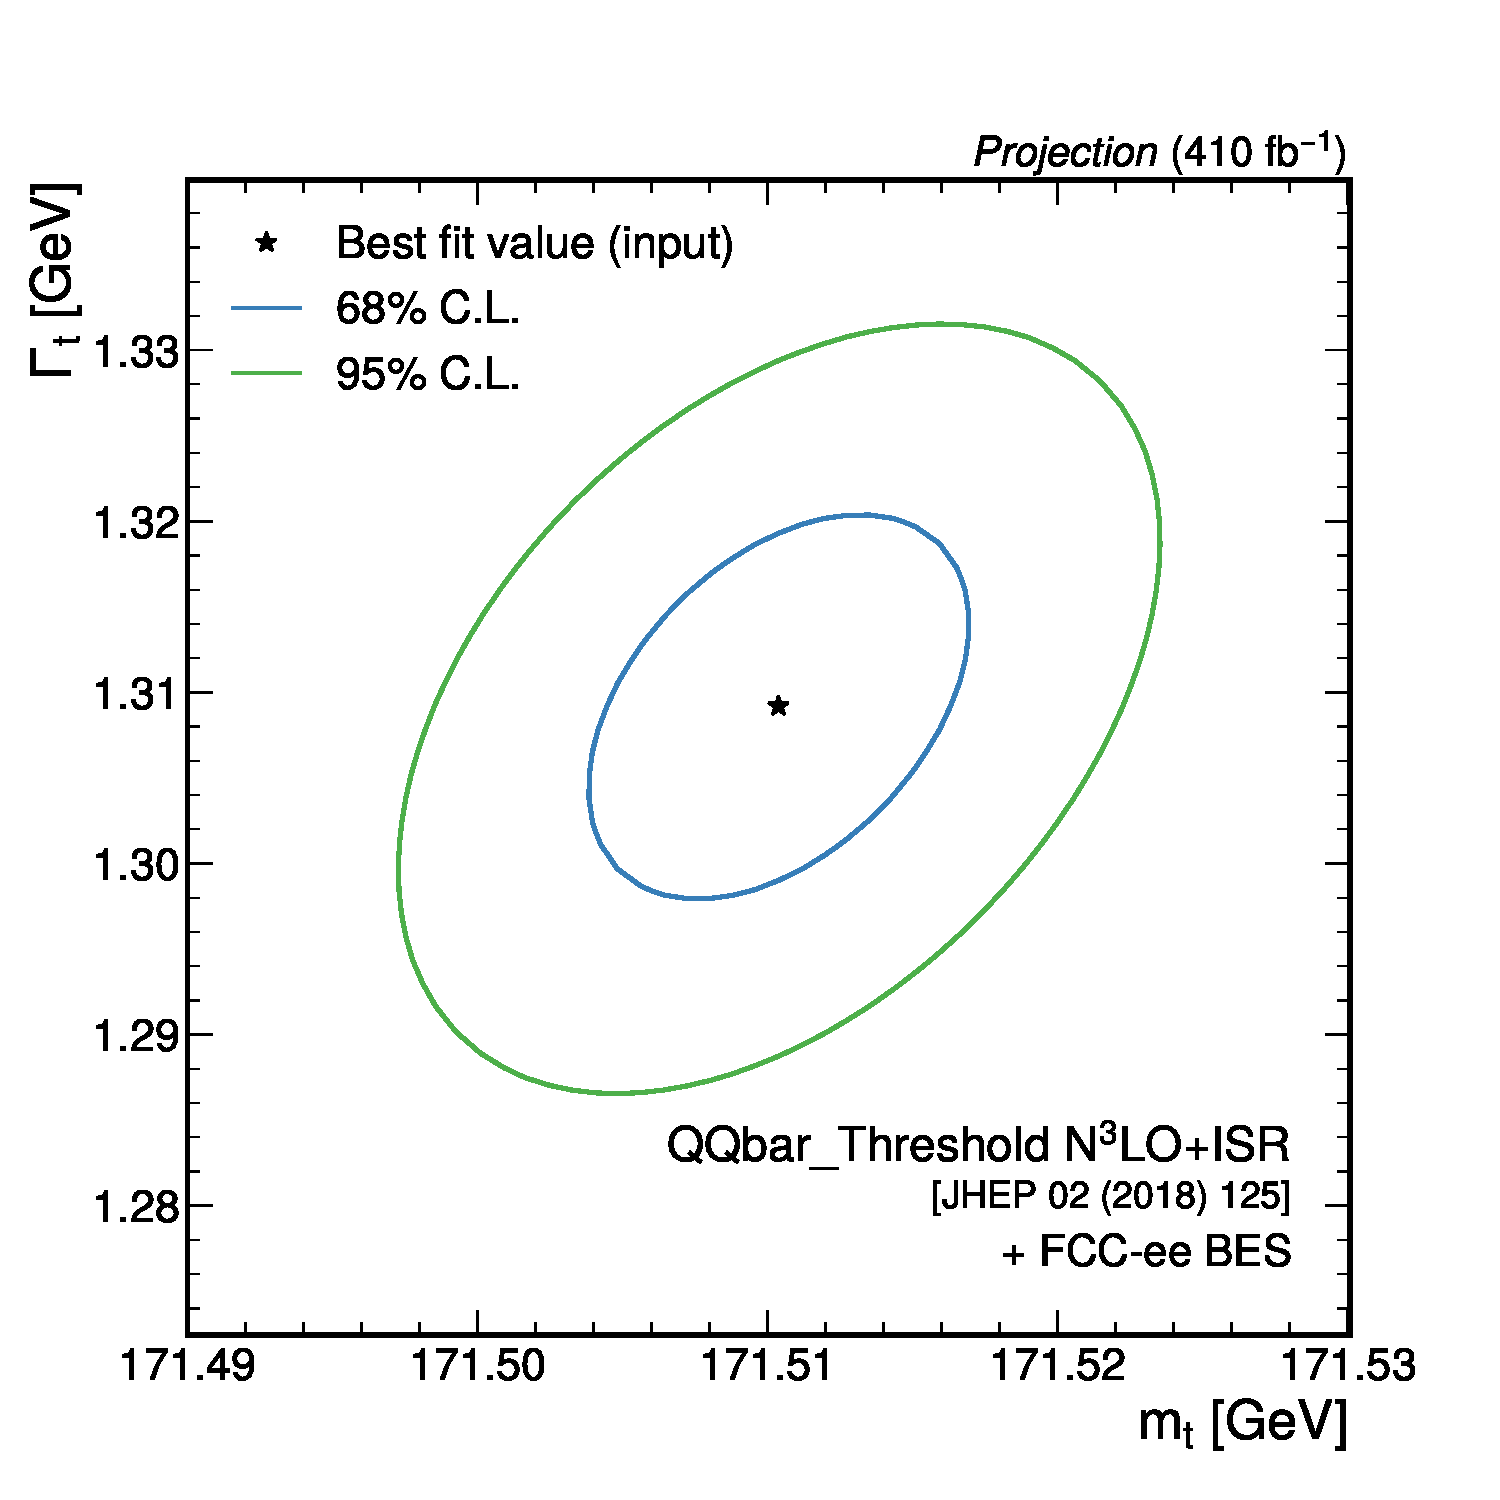
\includegraphics[width=0.75\textwidth]{Figs/scan/chi2_scan_mass_width.pdf}
  \caption{Two-parameter \(m_t\)-\(\Gamma_t\) likelihood structure for the top-threshold scan. Source: Ref.~\cite{DefranchisTopThreshold2025}.}
  \label{fig:top-chi2}
\end{figure}
The key lesson is that a projection is meaningful only after the measured observable, the assumptions entering its extraction, and the dominant uncertainty sources have been identified.

Figure~\ref{fig:top-alpha-uncert} is used here as a visual anchor for the surrounding discussion. The important point is not only the numerical projection shown in the figure, but also the way in which the relevant FCC observable is connected to a physical parameter of the Standard Model or to a possible deviation from it.
\begin{figure}[H]
  \centering
  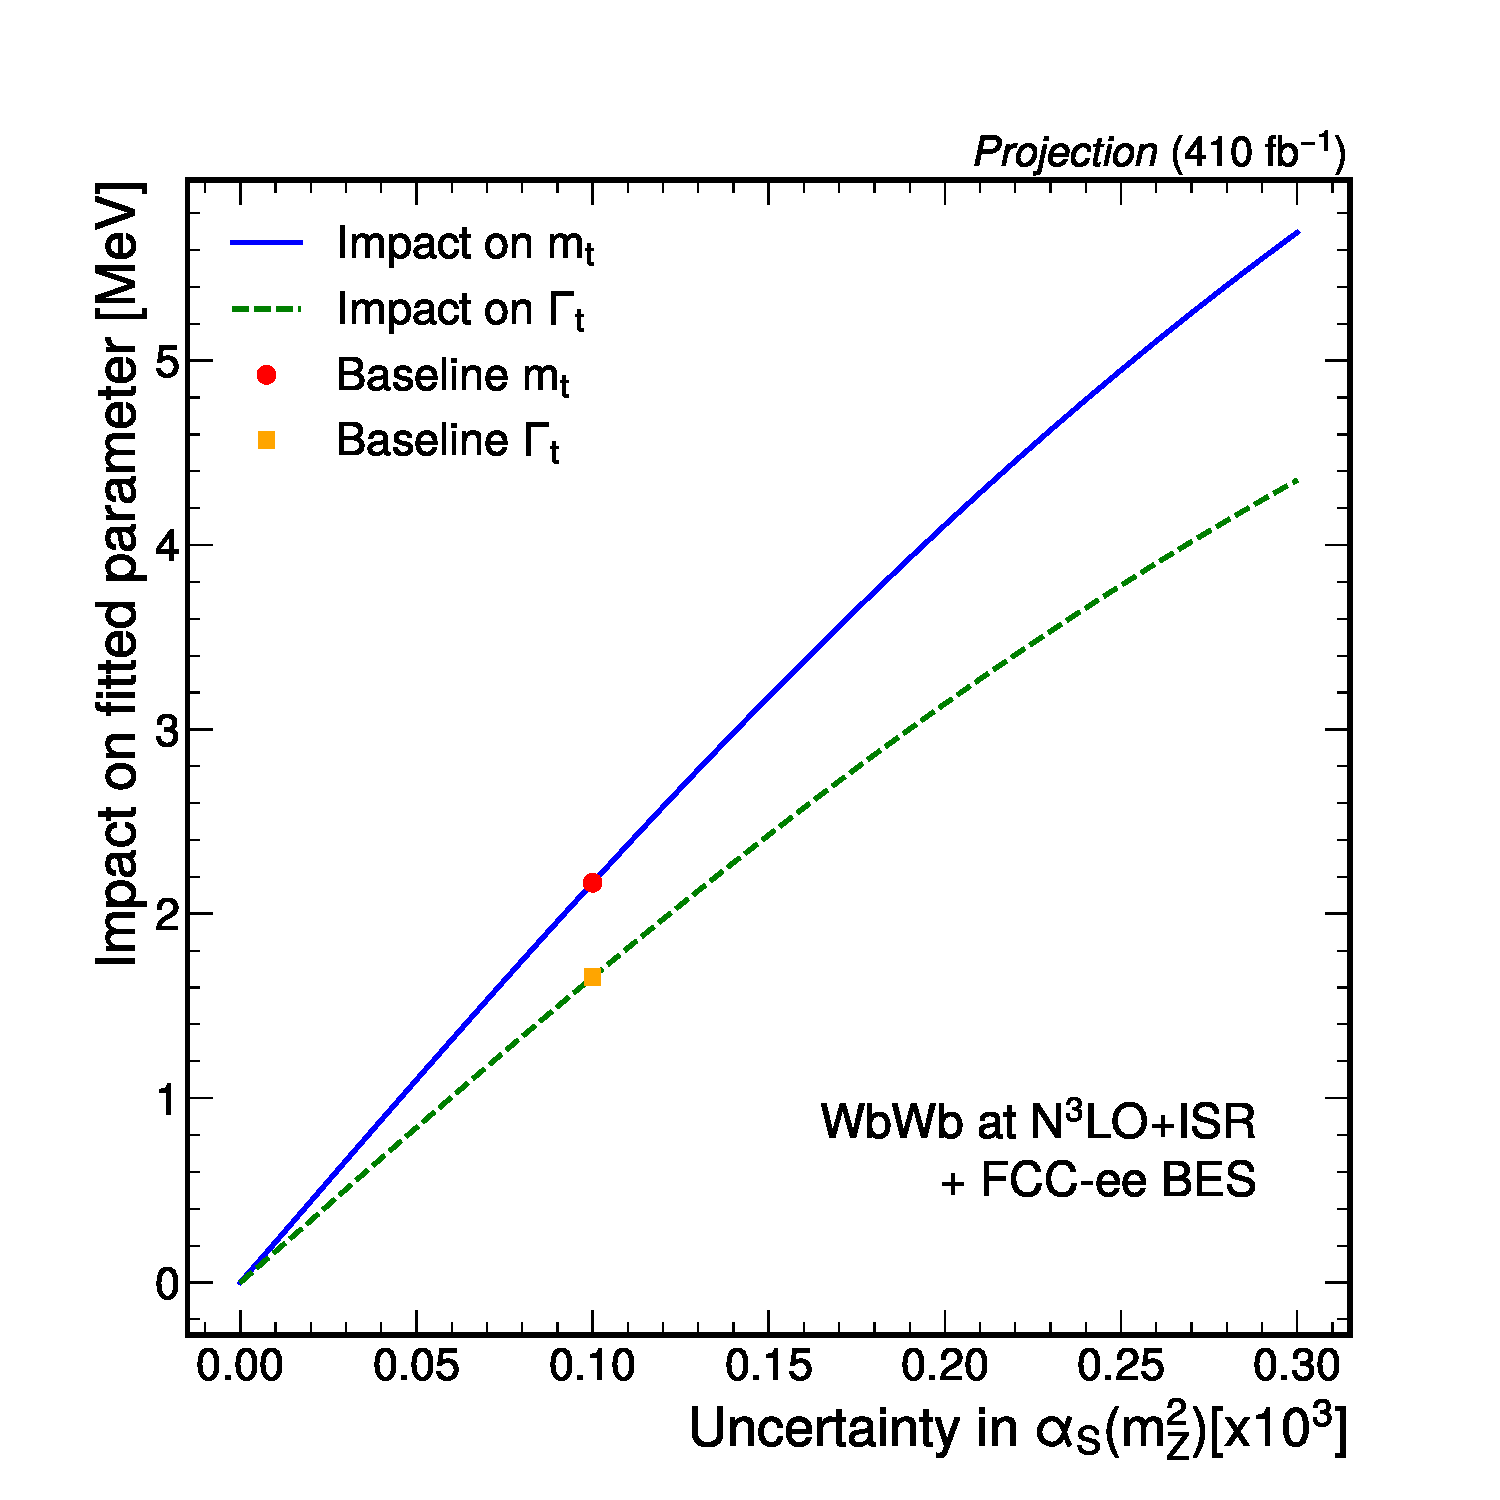
\includegraphics[width=0.75\textwidth]{Figs/scan/uncert_mass_width_vs_alphas.pdf}
  \caption{Parametric impact of the strong coupling on the top-threshold extraction. Source: Ref.~\cite{DefranchisTopThreshold2025}.}
  \label{fig:top-alpha-uncert}
\end{figure}
The key lesson is that a projection is meaningful only after the measured observable, the assumptions entering its extraction, and the dominant uncertainty sources have been identified.

\subsection{Top electroweak couplings at higher energy}
Above threshold, one can study
\begin{equation}
  e^+e^-\to \gamma^*,Z^*\to t\bar t .
\end{equation}
The Z-top interaction can be parametrised as
\begin{equation}
  \Lag_{ttZ}=\frac{g}{2c_W}\bar t\gamma^\mu\left(g_V^t-g_A^t\gamma_5\right)tZ_\mu .
\end{equation}
Angular distributions and polarisation-sensitive observables constrain deviations in \(g_V^t\), \(g_A^t\) and related EFT operators. The 365 GeV run is therefore not only an extension of the threshold scan; it probes the top electroweak sector directly.

Figure~\ref{fig:top-reco} is used here as a visual anchor for the surrounding discussion. The important point is not only the numerical projection shown in the figure, but also the way in which the relevant FCC observable is connected to a physical parameter of the Standard Model or to a possible deviation from it.
\begin{figure}[H]
  \centering
  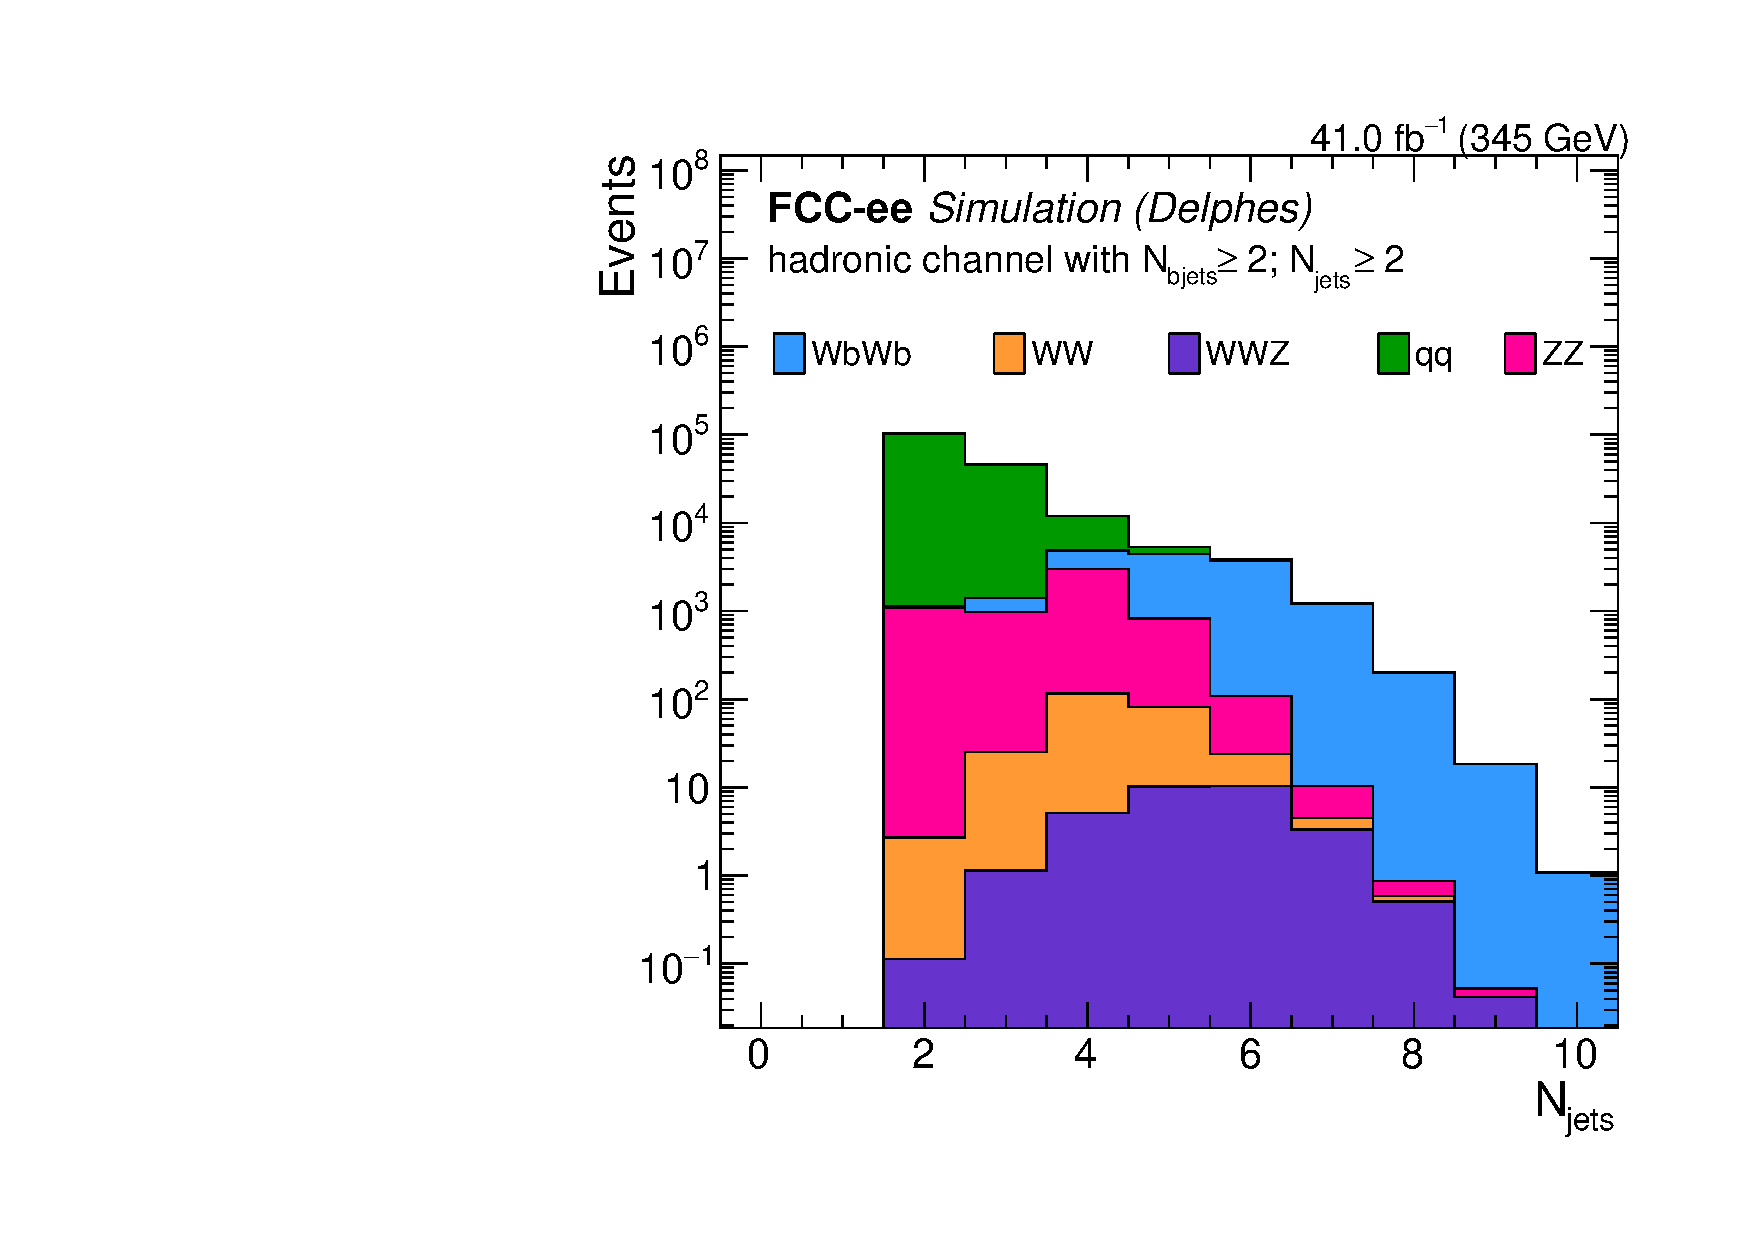
\includegraphics[width=0.78\textwidth]{Figs/reco/njgt1_effp9_twob_njets_R5_had_345_log.pdf}
  \caption{Example jet-multiplicity distribution in the hadronic \(WbWb\) final state with at least two b-tagged jets. Source: Ref.~\cite{DefranchisTopThreshold2025}.}
  \label{fig:top-reco}
\end{figure}
The key lesson is that a projection is meaningful only after the measured observable, the assumptions entering its extraction, and the dominant uncertainty sources have been identified.

Figure~\ref{fig:top-higgs-interplay} is used here as a visual anchor for the surrounding discussion. The important point is not only the numerical projection shown in the figure, but also the way in which the relevant FCC observable is connected to a physical parameter of the Standard Model or to a possible deviation from it.
\begin{figure}[H]
  \centering
  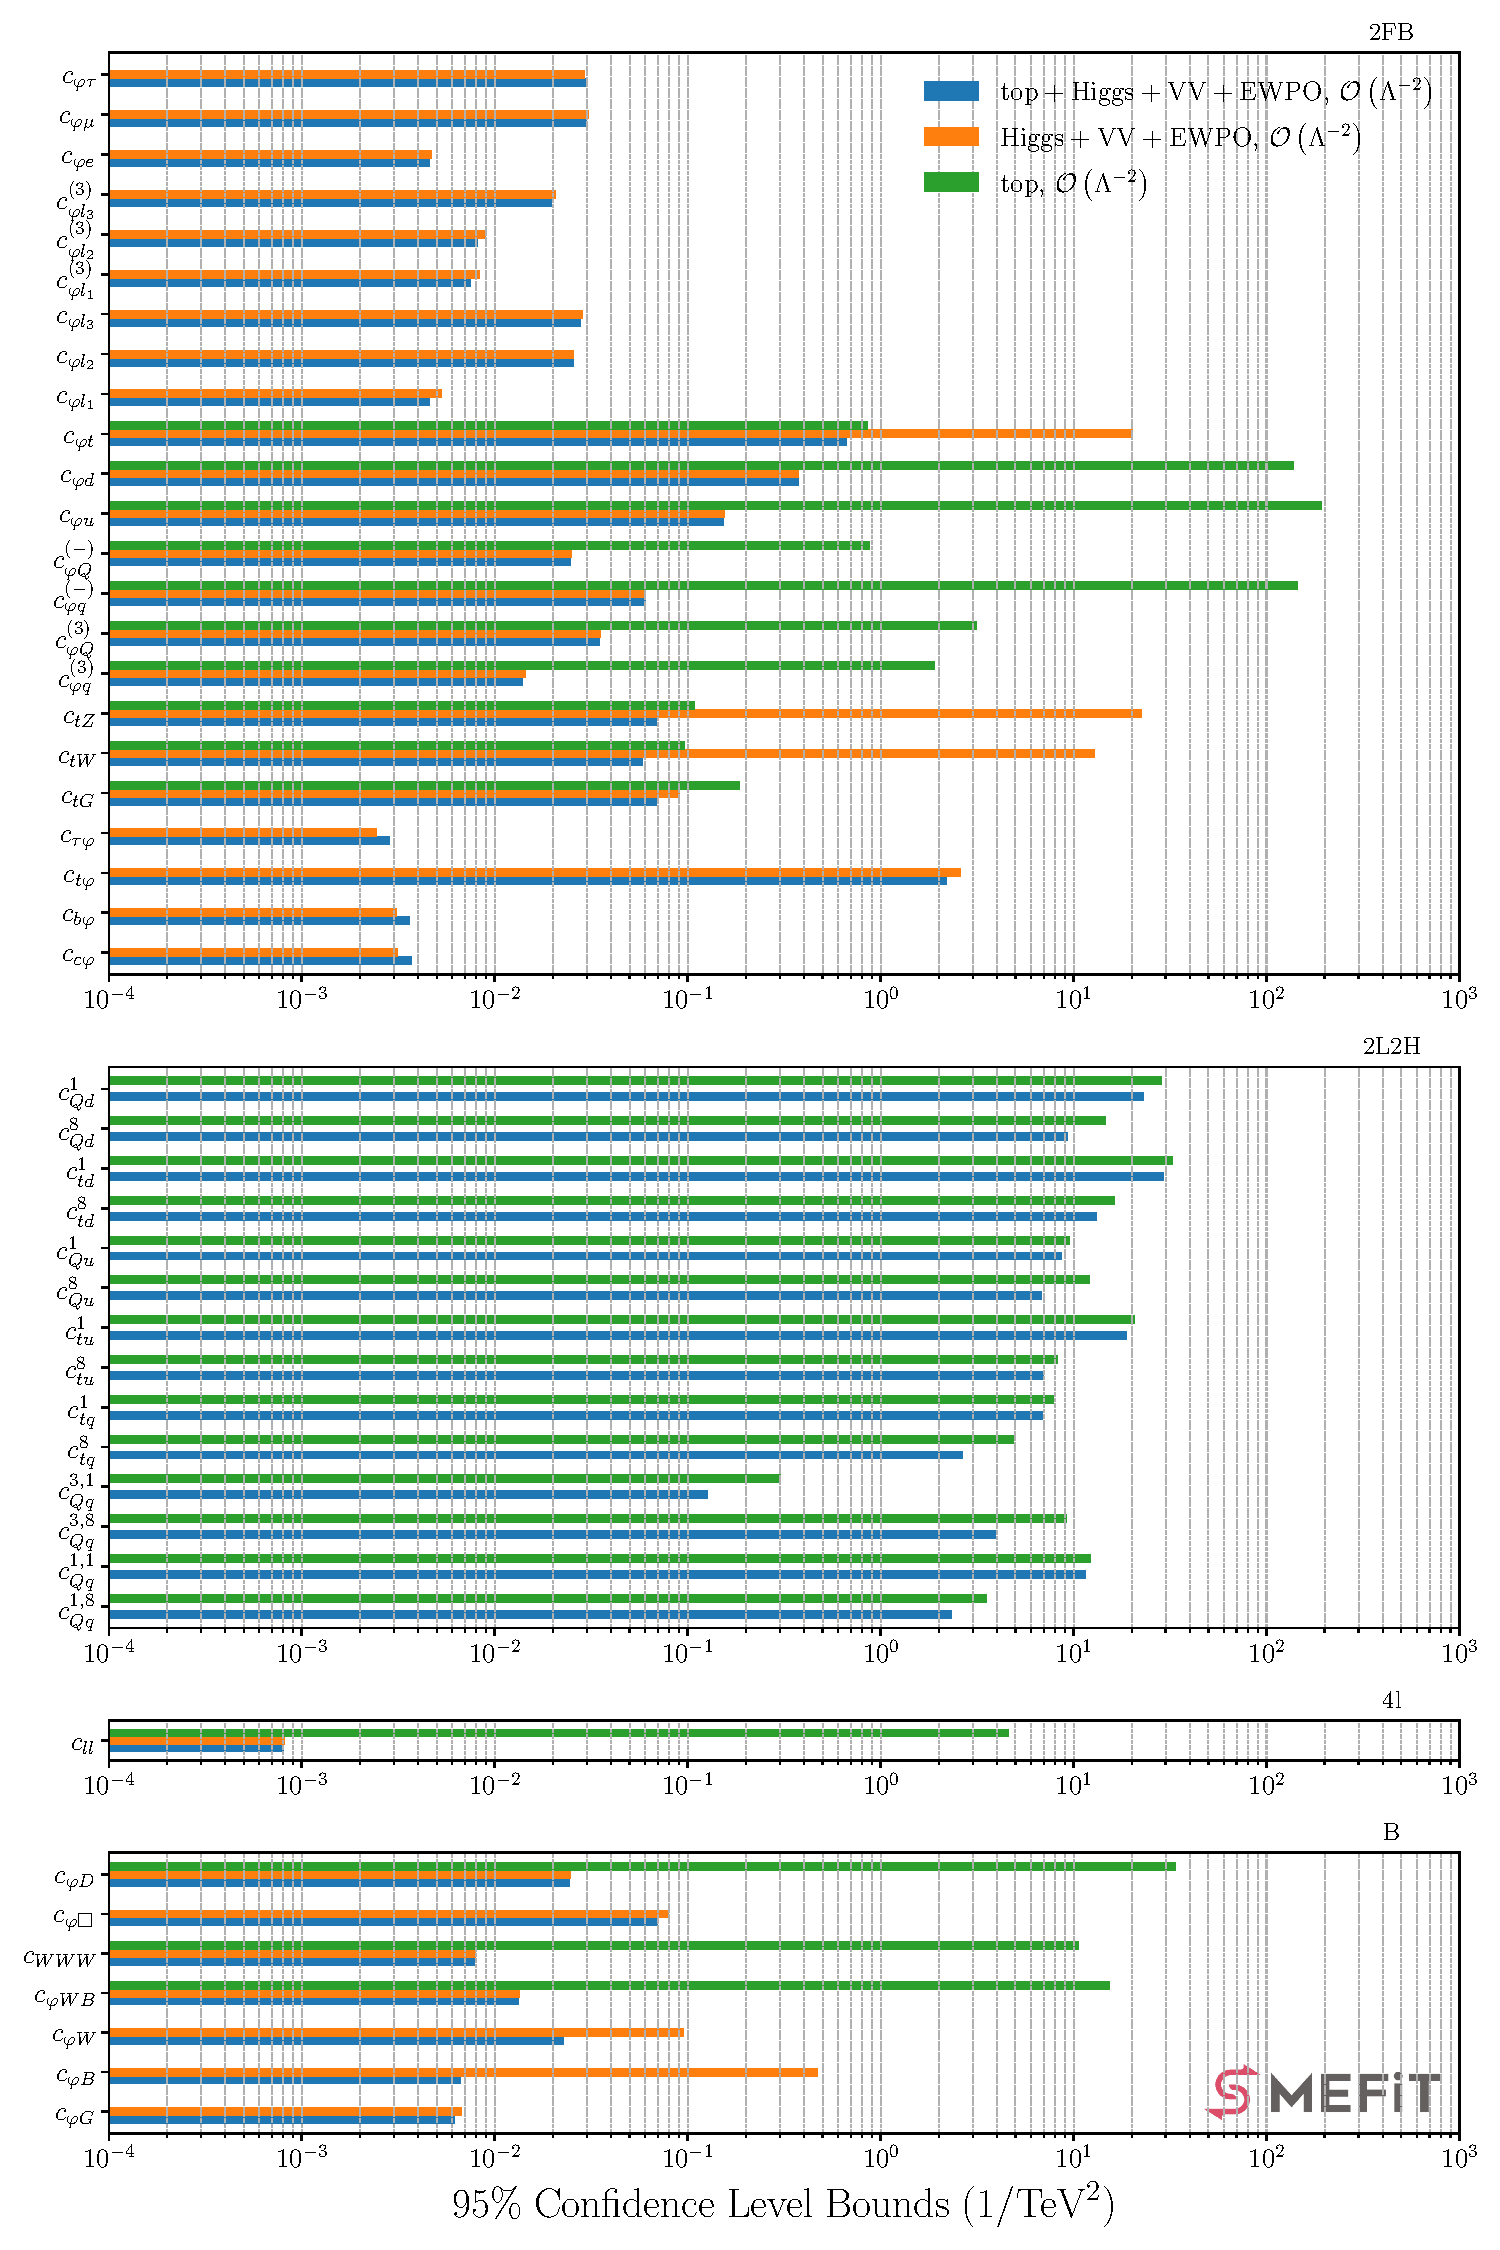
\includegraphics[width=0.85\textwidth]{Figs/Global_Interpretations/top-higgs-interplay-fcc.pdf}
  \caption{Interplay between Higgs and top measurements in global interpretations. Source: Ref.~\cite{ECFAFactories2025}.}
  \label{fig:top-higgs-interplay}
\end{figure}
The key lesson is that a projection is meaningful only after the measured observable, the assumptions entering its extraction, and the dominant uncertainty sources have been identified.

\subsection{Top FCNC as a rare-process case study}
Flavour-changing neutral currents in the top sector are highly suppressed in the Standard Model. Representative processes include
\begin{equation}
  e^+e^-\to t\bar q,\ \bar t q,
  \qquad
  t\to qZ,\quad t\to q\gamma,\quad t\to qH,
\end{equation}
where \(q=u,c\). Even if a detailed FCNC analysis is beyond the scope of this general lecture note, the topic illustrates the same logic as the rest of FCC precision physics: rare processes, clean event reconstruction and EFT interpretation combine to probe BSM flavour structures.

\begin{definition}{Top width}{top-width}
The top width \(\Gamma_t\) controls the lifetime of the top quark and enters the threshold line shape. Because the top decays before hadronising, \(\Gamma_t\) is accessible in a way that is qualitatively different from the widths of lighter quarks.
\end{definition}

\begin{examplebox}{Mass-scheme discipline}{mass-scheme-example}
A threshold scan may determine \(m_t^{\rm PS}(20\,\GeV)\) with a small experimental uncertainty. This number should not be quoted as a pole mass without a perturbative conversion and an associated theoretical uncertainty. Conversely, comparing it directly with a Monte-Carlo mass from hadron-collider reconstruction is conceptually misleading unless the scheme relation is specified.
\end{examplebox}

\begin{guidedchecksbox}
\begin{enumerate}[leftmargin=1.6em]
\item Explain why the threshold line shape is more sensitive to \(m_t\) through its horizontal position than through its normalisation.
\item Why are \(\alpha_s\) and \(y_t\) partially correlated in threshold observables?
\item List the experimental ingredients needed to separate \(WbWb\) signal from \(WW\), \(ZZ\), \(q\bar q\) and \(WWZ\) backgrounds.
\end{enumerate}
\end{guidedchecksbox}

\subsection{Exercises}
\begin{enumerate}[leftmargin=1.6em]
\item Explain why a top-threshold mass is theoretically cleaner than the pole mass for this measurement.
\item Describe how beam-energy spread modifies the apparent threshold line shape.
\item Write the leading EFT operators you would expect to affect \(e^+e^-\to t\bar t\) at 365 GeV.
\end{enumerate}


\newpage
\section{SMEFT and global interpretations}
\begin{guidelinebox}
This chapter turns the Higgs, electroweak and top measurements into a common interpretation problem. The SMEFT correlates observables that are often discussed separately. A credible FCC precision analysis therefore needs a global fit, not a list of independent coupling errors.
\end{guidelinebox}

\subsection{Operator classes}
Dimension-six SMEFT operators relevant for FCC-ee precision include bosonic operators, Higgs-current operators, Yukawa-like operators, dipoles, four-fermion operators and top operators. Schematically,
\begin{equation}
  \Lag_{\SMEFT}=\Lag_{\SM}+\sum_i c_iO_i,
\end{equation}
where the scale convention is absorbed into \(c_i\), or equivalently
\begin{equation}
  \Lag_{\SMEFT}=\Lag_{\SM}+\sum_i\frac{C_i}{\Lambda^2}O_i .
\end{equation}
Examples include
\begin{align}
  O_{\phi D}&=(\phi^\dagger D^\mu\phi)^*(\phi^\dagger D_\mu\phi),\\
  O_{\phi WB}&=(\phi^\dagger\tau^I\phi)W^I_{\mu\nu}B^{\mu\nu},\\
  O_{u\phi}&=(\phi^\dagger\phi)(\bar q u\tilde\phi),\\
  O_{\ell\ell}&=(\bar\ell\gamma_\mu\ell)(\bar\ell\gamma^\mu\ell).
\end{align}
Each of these examples affects more than one observable, which is why correlations are essential.

Figure~\ref{fig:smeft-coefficients-2} is used here as a visual anchor for the surrounding discussion. The important point is not only the numerical projection shown in the figure, but also the way in which the relevant FCC observable is connected to a physical parameter of the Standard Model or to a possible deviation from it.
\begin{figure}[H]
  \centering
  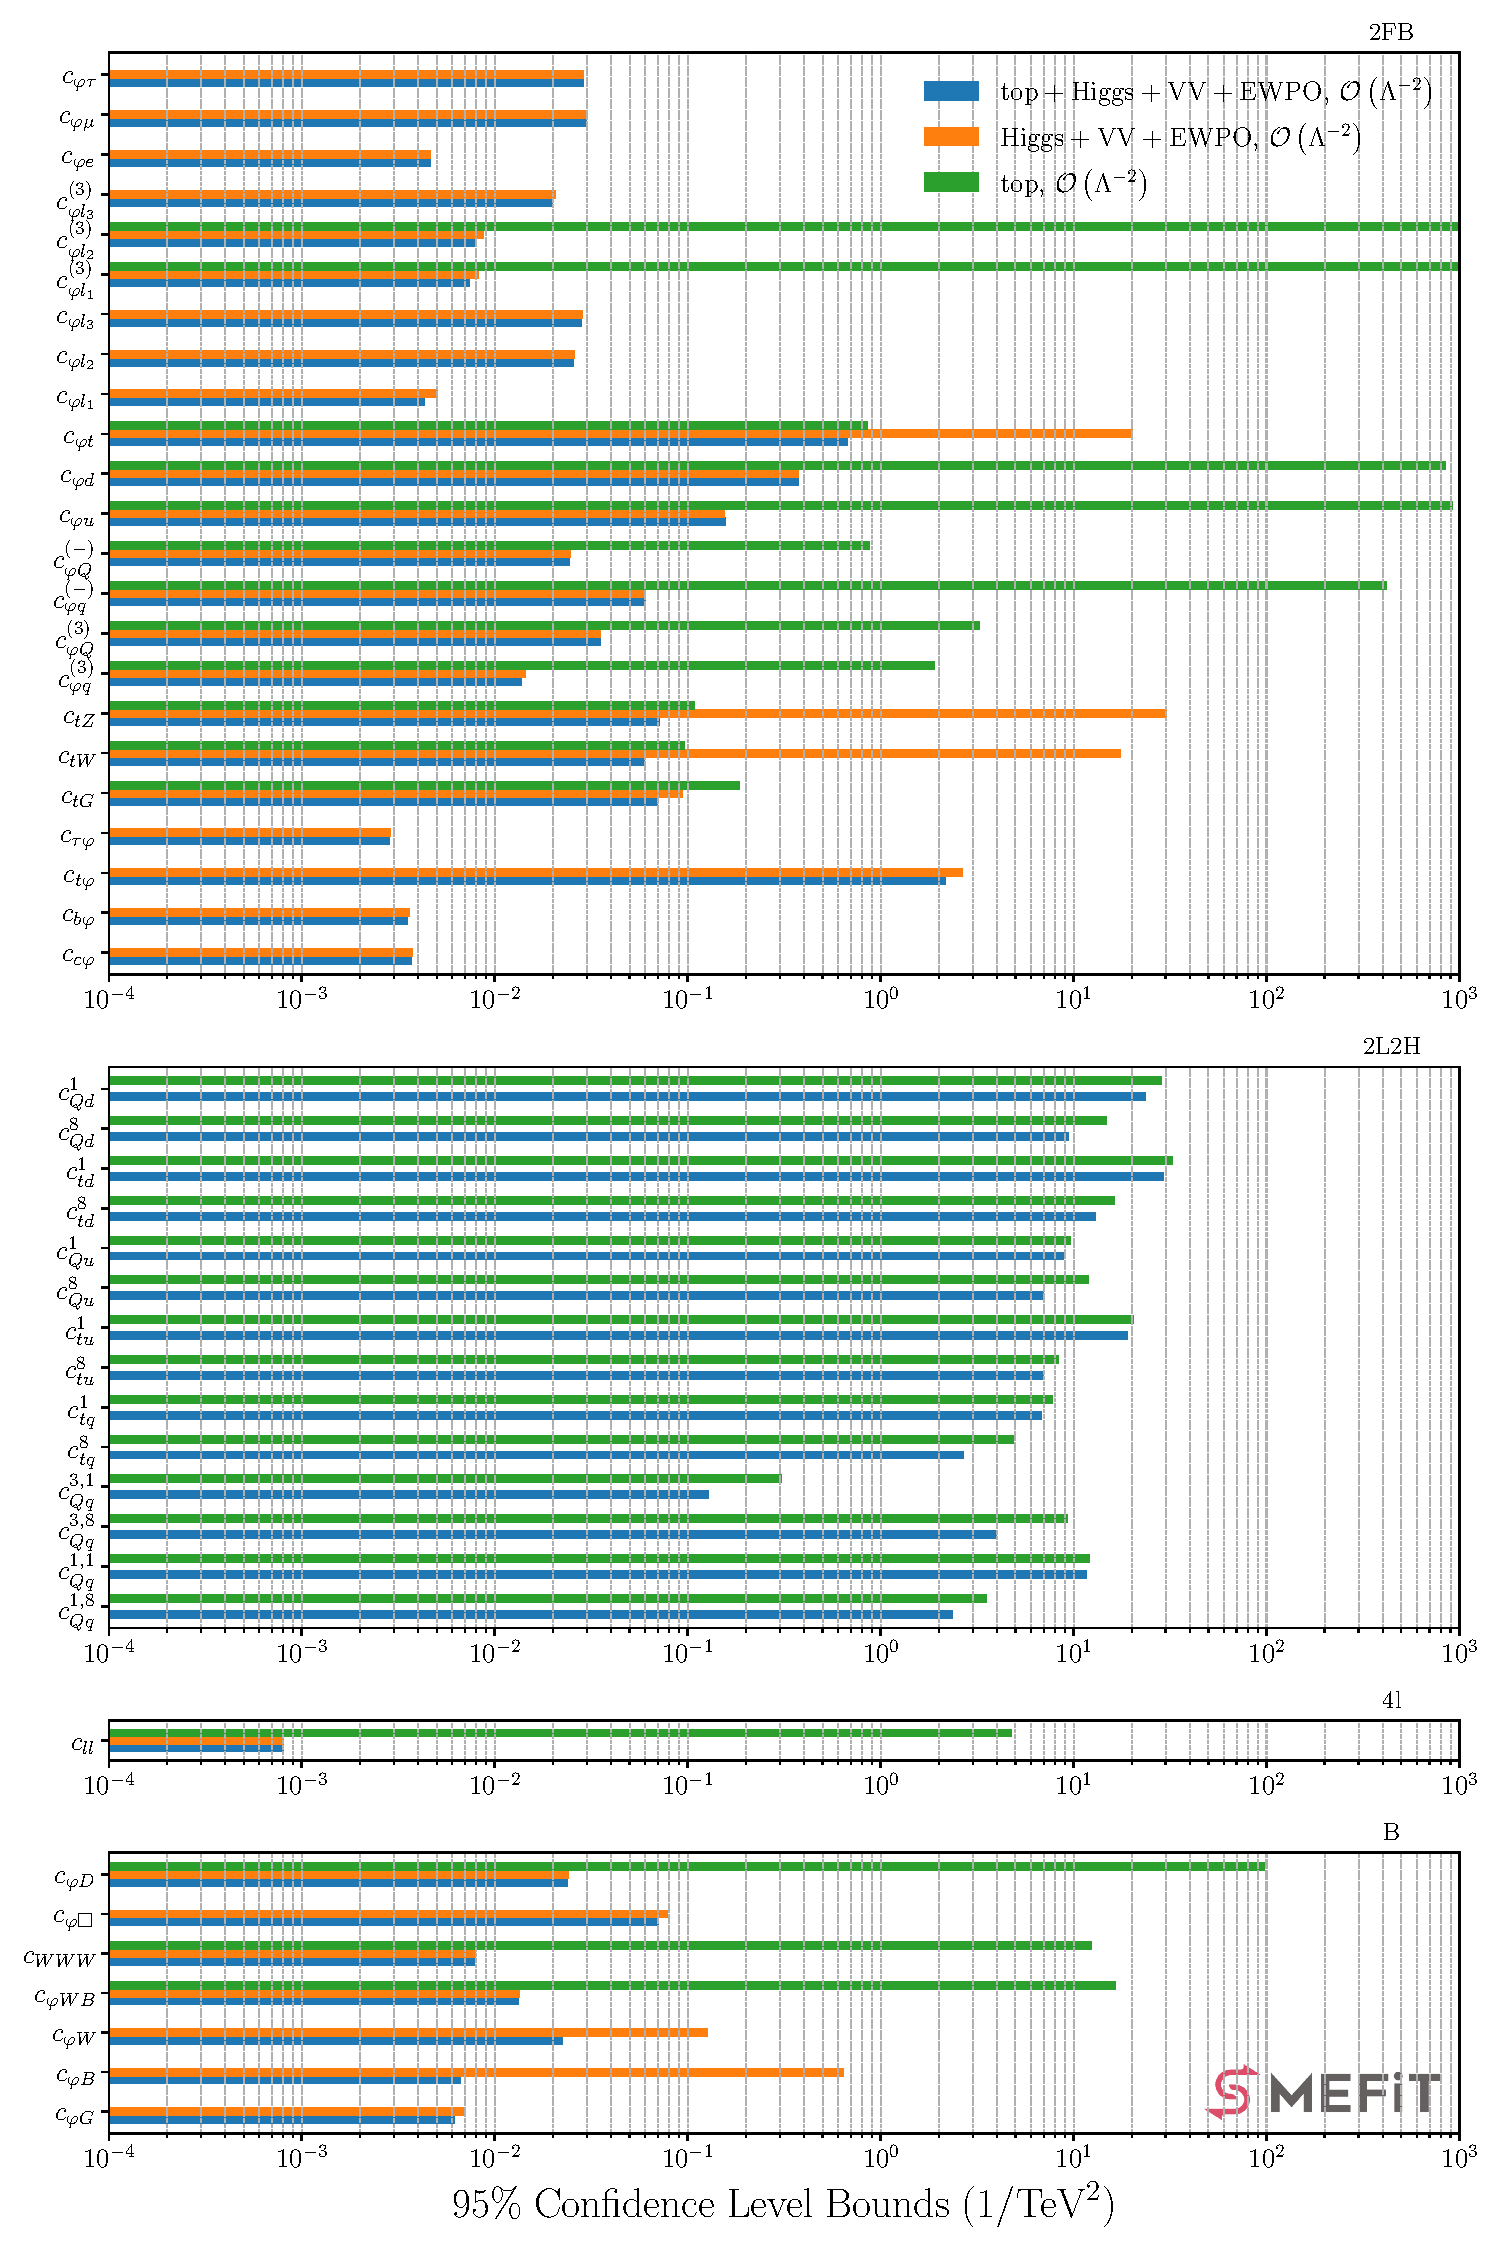
\includegraphics[width=0.92\textwidth]{Figs/Global_Interpretations/coefficient_bar_final.pdf}
  \caption{Representative global SMEFT coefficient constraints from future collider inputs. Source: Ref.~\cite{ArmadilloSMEFiT2026}.}
  \label{fig:smeft-coefficients-2}
\end{figure}
The key lesson is that a projection is meaningful only after the measured observable, the assumptions entering its extraction, and the dominant uncertainty sources have been identified.

Figure~\ref{fig:smeft-bar-2} is used here as a visual anchor for the surrounding discussion. The important point is not only the numerical projection shown in the figure, but also the way in which the relevant FCC observable is connected to a physical parameter of the Standard Model or to a possible deviation from it.
\begin{figure}[H]
  \centering
  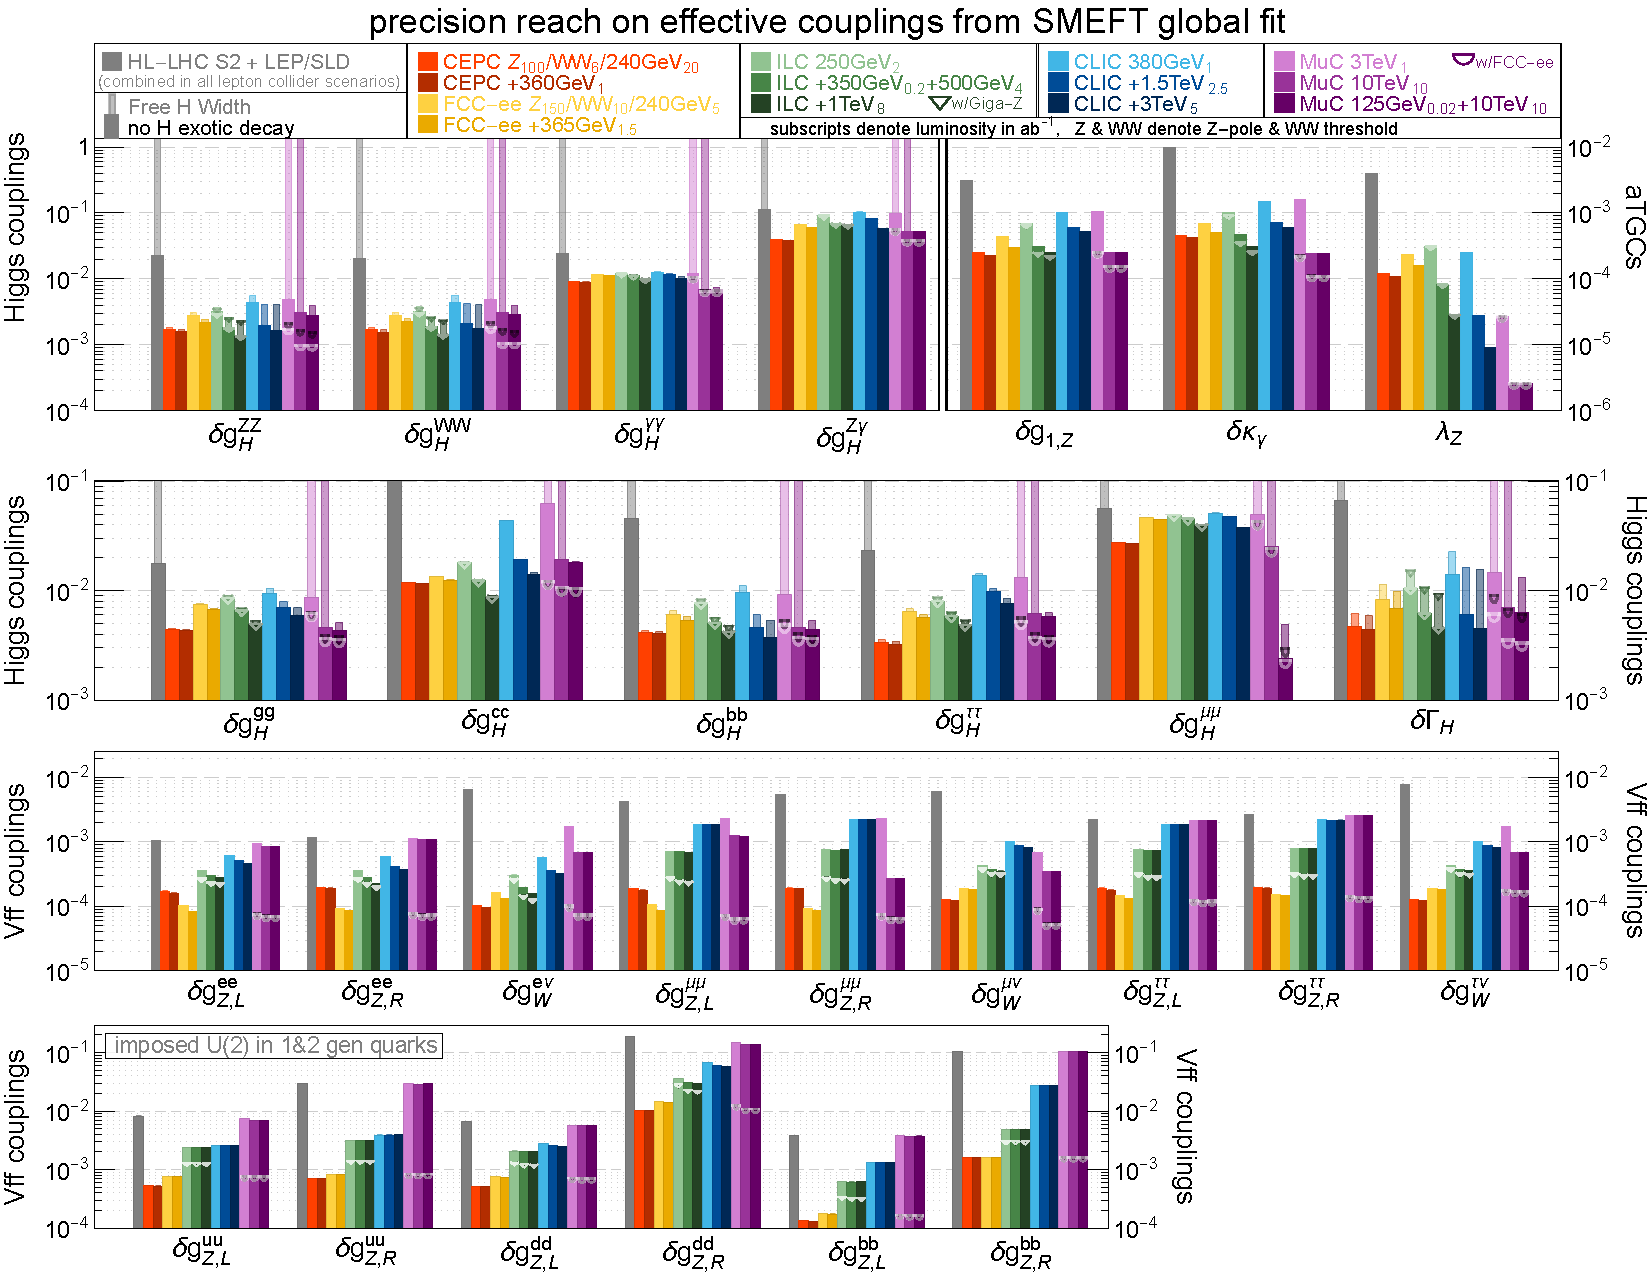
\includegraphics[width=0.92\textwidth]{Figs/Global_Interpretations/barplotsnow-xo1-smpar.pdf}
  \caption{Comparison of projected precision in a global interpretation framework. Source: Ref.~\cite{ECFAFactories2025}.}
  \label{fig:smeft-bar-2}
\end{figure}
The key lesson is that a projection is meaningful only after the measured observable, the assumptions entering its extraction, and the dominant uncertainty sources have been identified.

Figure~\ref{fig:smeft-uv-spider-2} is used here as a visual anchor for the surrounding discussion. The important point is not only the numerical projection shown in the figure, but also the way in which the relevant FCC observable is connected to a physical parameter of the Standard Model or to a possible deviation from it.
\begin{figure}[H]
  \centering
  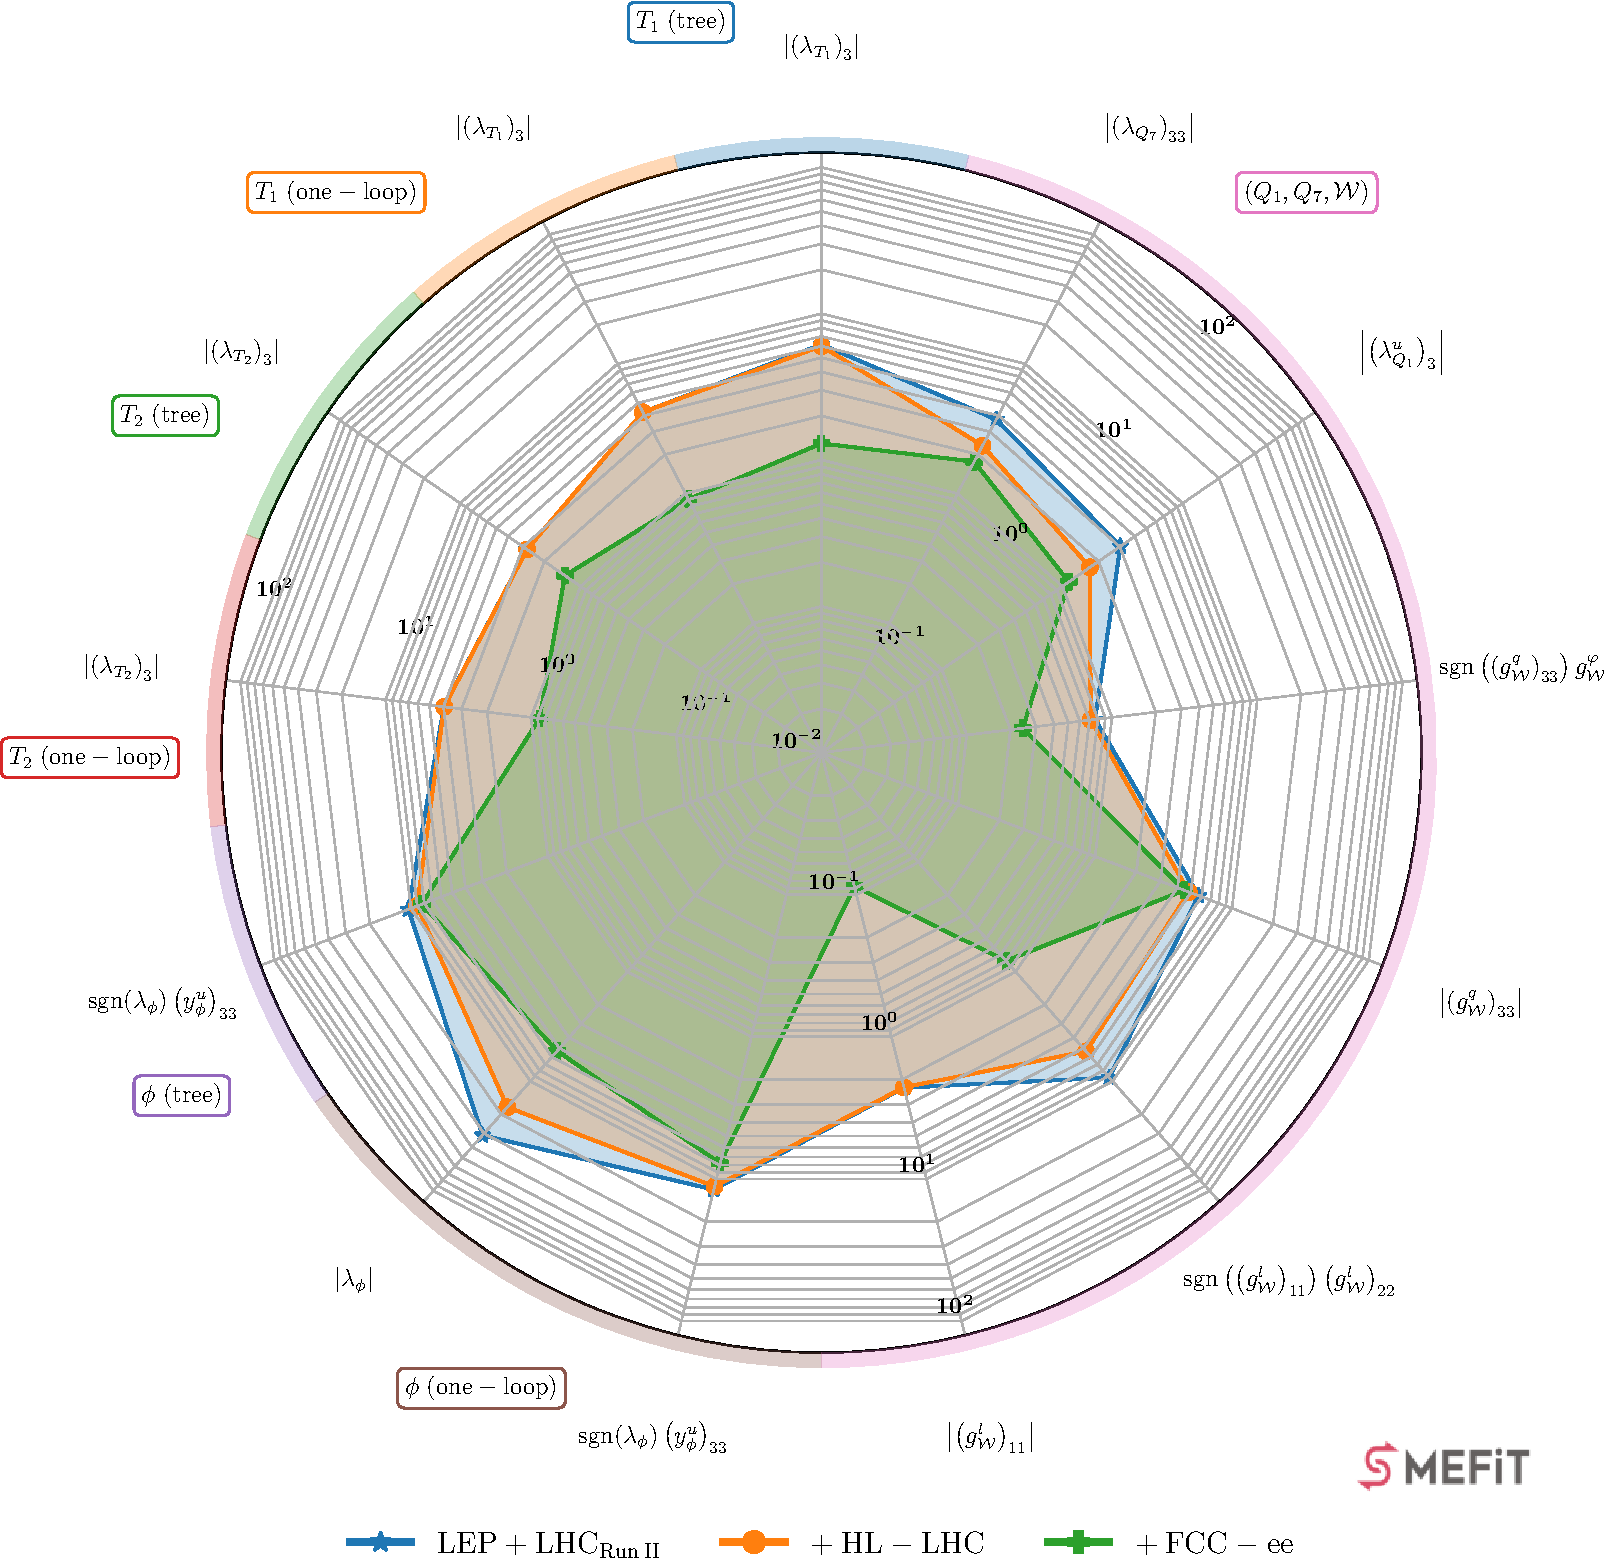
\includegraphics[width=0.88\textwidth]{Figs/Global_Interpretations/spider_plot_uv.pdf}
  \caption{FCC-ee constraints on representative UV models matched onto the SMEFT. Source: Ref.~\cite{ArmadilloSMEFiT2026}.}
  \label{fig:smeft-uv-spider-2}
\end{figure}
The key lesson is that a projection is meaningful only after the measured observable, the assumptions entering its extraction, and the dominant uncertainty sources have been identified.

\subsection{Observable expansion and fit logic}
A general observable can be expanded as
\begin{equation}
  \mathcal O_a(\vec C)=\mathcal O_{a,\SM}
  +\sum_i C_i\,\mathcal O_{a,i}^{(6)}
  +\sum_{ij}C_iC_j\,\mathcal O_{a,ij}^{(6,6)}+\cdots .
\end{equation}
A Gaussian approximation to the likelihood has the form
\begin{equation}
  \chi^2(\vec C)=
  \left[\vec O_{\rm exp}-\vec O_{\rm th}(\vec C)\right]^T
  V^{-1}
  \left[\vec O_{\rm exp}-\vec O_{\rm th}(\vec C)\right],
\end{equation}
where \(V\) is the covariance matrix. More refined analyses include non-Gaussian likelihoods, nuisance parameters and theory-covariance assumptions.

\begin{definition}{Global SMEFT fit}{global-fit}
A global SMEFT fit simultaneously constrains many Wilson coefficients using many observables. The purpose is not simply to obtain smaller error bars, but to correctly account for correlations, degeneracies and the fact that gauge invariance links Higgs, electroweak, top and diboson measurements.
\end{definition}

\subsection{Effective couplings and pseudo-observables}
Between the kappa framework and the full SMEFT lies an effective-coupling description. Higgs effective couplings can be defined through partial widths, for example
\begin{equation}
  g_{HX}^{\rm eff}=\sqrt{\frac{\Gamma(H\to X)}{\Gamma(H\to X)_{\SM}}} .
\end{equation}
Similarly, electroweak effective couplings describe shifts in Z and W couplings to fermions. These quantities are experimentally intuitive and closer to pseudo-observables, but the SMEFT dictionary is needed to connect them to gauge-invariant operator coefficients.

Figure~\ref{fig:higgs-fermion-eff-2} is used here as a visual anchor for the surrounding discussion. The important point is not only the numerical projection shown in the figure, but also the way in which the relevant FCC observable is connected to a physical parameter of the Standard Model or to a possible deviation from it.
\begin{figure}[H]
  \centering
  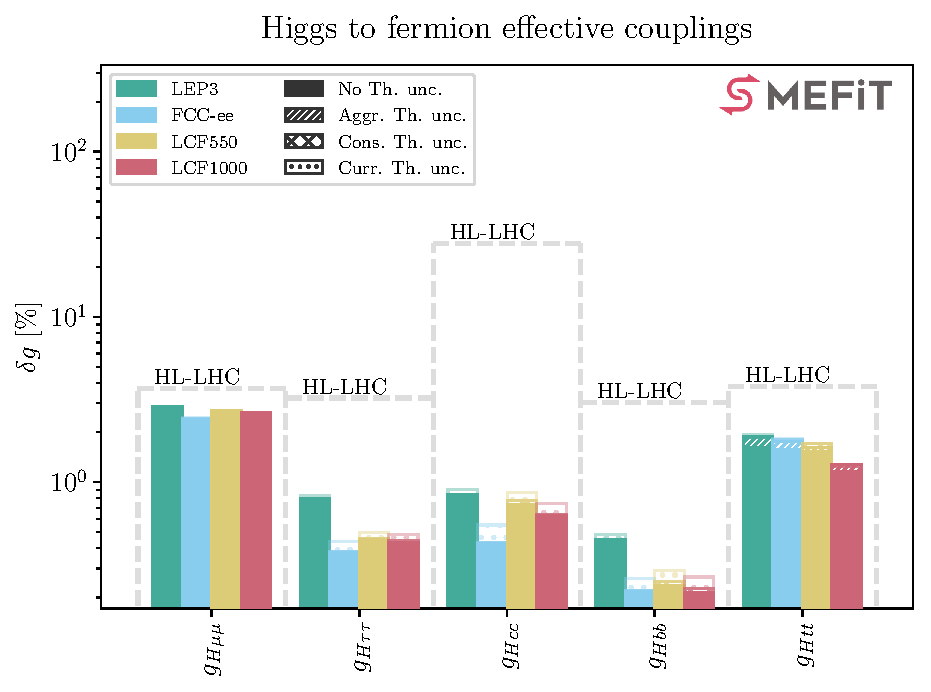
\includegraphics[width=0.78\textwidth]{Figs/Higgs_to_fermion_effective_couplings.pdf}
  \caption{Projected constraints on effective Higgs couplings to fermions. Source: Ref.~\cite{ArmadilloSMEFiT2026}.}
  \label{fig:higgs-fermion-eff-2}
\end{figure}
The key lesson is that a projection is meaningful only after the measured observable, the assumptions entering its extraction, and the dominant uncertainty sources have been identified.

Figure~\ref{fig:higgs-vector-eff-2} is used here as a visual anchor for the surrounding discussion. The important point is not only the numerical projection shown in the figure, but also the way in which the relevant FCC observable is connected to a physical parameter of the Standard Model or to a possible deviation from it.
\begin{figure}[H]
  \centering
  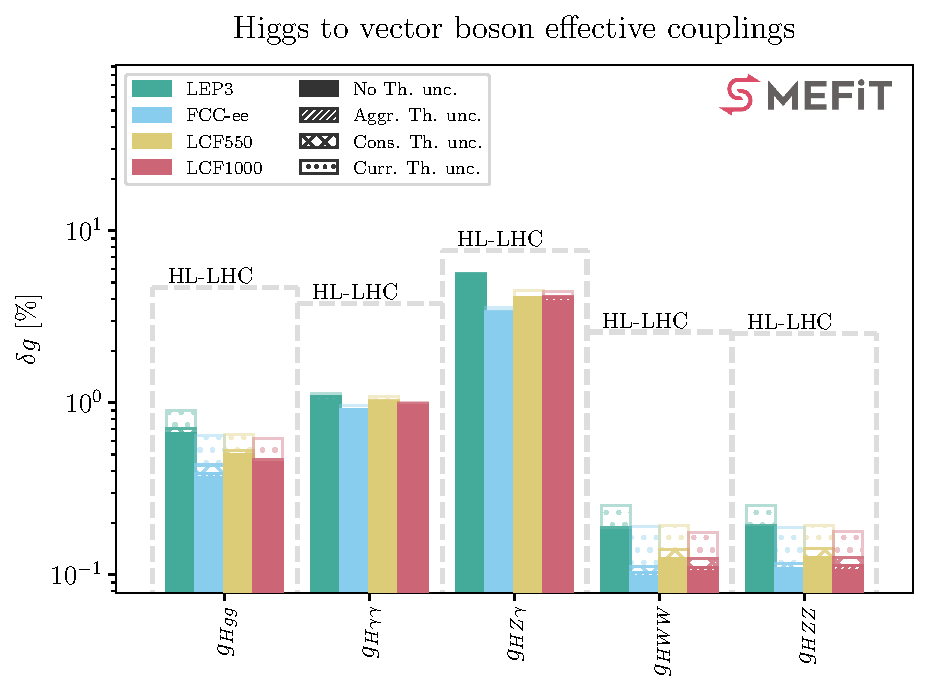
\includegraphics[width=0.78\textwidth]{Figs/Higgs_to_vector_boson_effective_couplings.pdf}
  \caption{Projected constraints on effective Higgs couplings to electroweak vector bosons. Source: Ref.~\cite{ArmadilloSMEFiT2026}.}
  \label{fig:higgs-vector-eff-2}
\end{figure}
The key lesson is that a projection is meaningful only after the measured observable, the assumptions entering its extraction, and the dominant uncertainty sources have been identified.

Figure~\ref{fig:w-effective-couplings-2} is used here as a visual anchor for the surrounding discussion. The important point is not only the numerical projection shown in the figure, but also the way in which the relevant FCC observable is connected to a physical parameter of the Standard Model or to a possible deviation from it.
\begin{figure}[H]
  \centering
  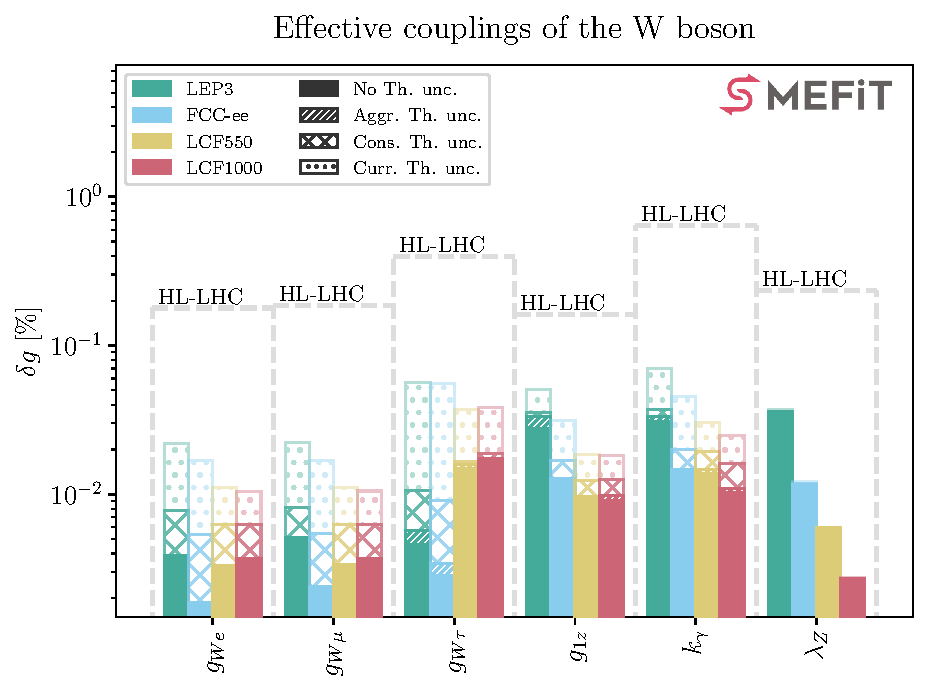
\includegraphics[width=0.78\textwidth]{Figs/Effective_couplings_of_the_W_boson.pdf}
  \caption{Projected constraints on effective W-boson couplings in future collider fits. Source: Ref.~\cite{ArmadilloSMEFiT2026}.}
  \label{fig:w-effective-couplings-2}
\end{figure}
The key lesson is that a projection is meaningful only after the measured observable, the assumptions entering its extraction, and the dominant uncertainty sources have been identified.

\subsection{UV matching and model interpretation}
Once a SMEFT fit constrains Wilson coefficients, a UV model can be matched onto those coefficients. If a heavy scalar, vector or fermion is integrated out, the resulting pattern of operators depends on its quantum numbers and couplings. Two models with similar mass reach in a direct search can have very different indirect footprints. Conversely, two very different UV models can generate similar low-energy coefficient patterns, producing degeneracies that only additional observables can resolve.

Figure~\ref{fig:new-scalars-2} is used here as a visual anchor for the surrounding discussion. The important point is not only the numerical projection shown in the figure, but also the way in which the relevant FCC observable is connected to a physical parameter of the Standard Model or to a possible deviation from it.
\begin{figure}[H]
  \centering
  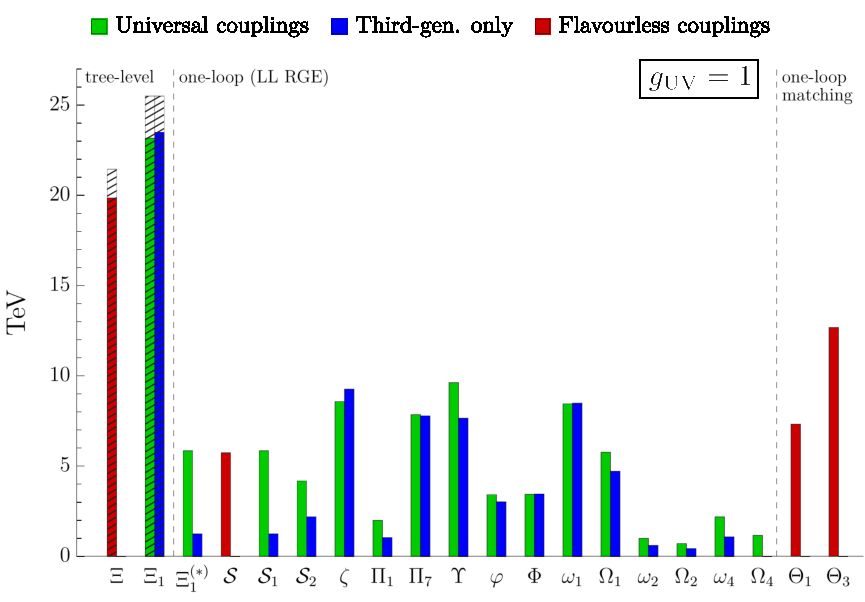
\includegraphics[width=0.88\textwidth]{Figs/Global_Interpretations/newscalars.pdf}
  \caption{Mass reach for representative new scalar fields inferred from precision observables and SMEFT matching. Source: Ref.~\cite{ECFAFactories2025}.}
  \label{fig:new-scalars-2}
\end{figure}
The key lesson is that a projection is meaningful only after the measured observable, the assumptions entering its extraction, and the dominant uncertainty sources have been identified.

Figure~\ref{fig:new-fermions-2} is used here as a visual anchor for the surrounding discussion. The important point is not only the numerical projection shown in the figure, but also the way in which the relevant FCC observable is connected to a physical parameter of the Standard Model or to a possible deviation from it.
\begin{figure}[H]
  \centering
  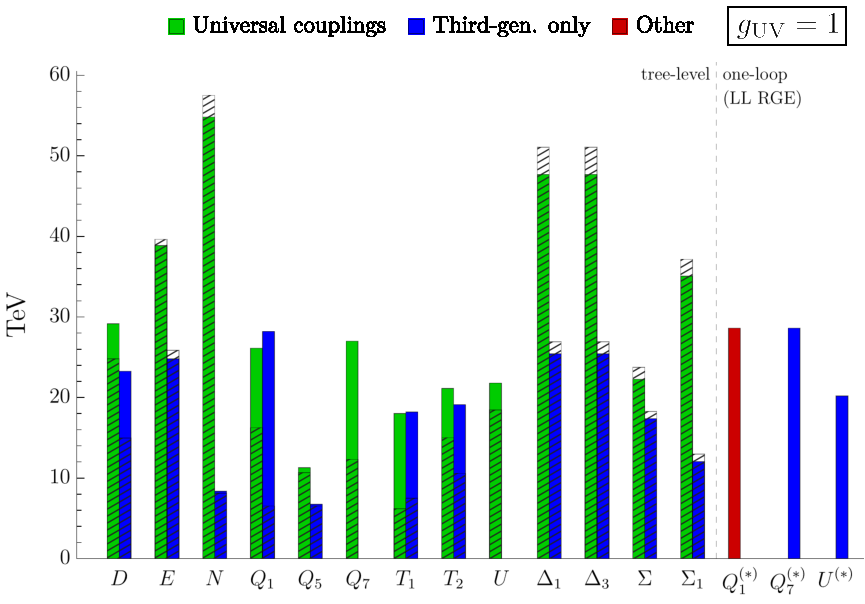
\includegraphics[width=0.88\textwidth]{Figs/Global_Interpretations/newfermions.pdf}
  \caption{Mass reach for representative new fermion fields inferred from precision observables and SMEFT matching. Source: Ref.~\cite{ECFAFactories2025}.}
  \label{fig:new-fermions-2}
\end{figure}
The key lesson is that a projection is meaningful only after the measured observable, the assumptions entering its extraction, and the dominant uncertainty sources have been identified.

Figure~\ref{fig:new-vectors-2} is used here as a visual anchor for the surrounding discussion. The important point is not only the numerical projection shown in the figure, but also the way in which the relevant FCC observable is connected to a physical parameter of the Standard Model or to a possible deviation from it.
\begin{figure}[H]
  \centering
  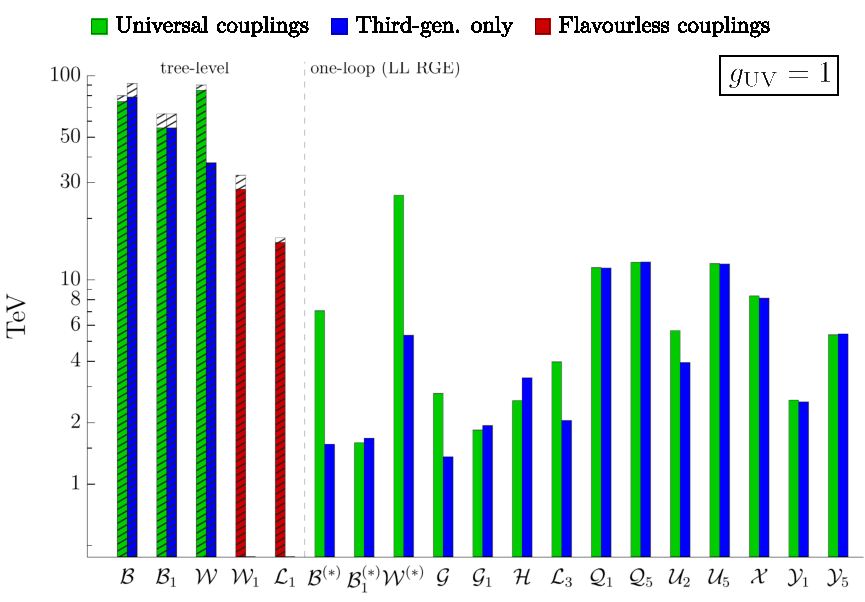
\includegraphics[width=0.88\textwidth]{Figs/Global_Interpretations/newvectorslog.pdf}
  \caption{Mass reach for representative new vector fields inferred from precision observables and SMEFT matching. Source: Ref.~\cite{ECFAFactories2025}.}
  \label{fig:new-vectors-2}
\end{figure}
The key lesson is that a projection is meaningful only after the measured observable, the assumptions entering its extraction, and the dominant uncertainty sources have been identified.

\begin{remarkbox}{A single coupling deviation is rarely enough}{single-deviation}
A deviation in a Higgs coupling should not be interpreted in isolation. The same new physics may shift Z-pole observables, WW production, top couplings and four-fermion contact interactions. The pattern of deviations is usually more informative than any single number.
\end{remarkbox}

\begin{guidedchecksbox}
\begin{enumerate}[leftmargin=1.6em]
\item Why can \(O_{\phi WB}\) affect both electroweak precision observables and Higgs processes?
\item Explain the difference between a kappa modifier and a SMEFT Wilson coefficient.
\item What information is lost when only marginalised one-dimensional coefficient bounds are quoted?
\end{enumerate}
\end{guidedchecksbox}

\subsection{Exercises}
\begin{enumerate}[leftmargin=1.6em]
\item Write the schematic effect of a four-fermion operator on \(e^+e^-\to f\bar f\) and explain why high-energy data help.
\item Compare the interpretation of \(\kappa_Z\\neq1\) in the kappa framework and in SMEFT.
\item Choose one UV mass-reach figure and explain which assumptions are needed to translate a Wilson-coefficient bound into a particle-mass bound.
\end{enumerate}


\newpage
\section{Flavour and tau physics at the Z pole}
\begin{guidelinebox}
The Tera-Z programme turns FCC-ee into a heavy-flavour and tau factory, as developed in the FCC flavour and tau studies~\cite{WilkinsonFlavour2025,WilkinsonHeavyQuark2021,DamTau2021}. The clean environment, large boost of heavy hadrons, high statistics and excellent vertexing create opportunities that are complementary to LHCb, Belle II and fixed-target experiments.
\end{guidelinebox}

\subsection{Heavy flavour at the Z pole}
At the Z pole, the processes
\begin{equation}
  e^+e^-\to Z\to b\bar b,
  \qquad
  e^+e^-\to Z\to c\bar c
\end{equation}
produce enormous samples of heavy hadrons. These samples can be used for rare decays, CP violation, lepton-universality tests and searches for forbidden transitions. The clean event environment helps modes with neutral particles, photons, missing energy and tau leptons.

\begin{definition}{Flavour-changing neutral current}{fcnc-def}
A flavour-changing neutral current is a transition in which the flavour of a quark or lepton changes without changing electric charge, such as \(b\to s\) or \(t\to c\) through a neutral mediator. In the Standard Model these processes are absent at tree level and suppressed by loops and flavour mixing, making them sensitive probes of new physics.
\end{definition}

Representative rare transitions include
\begin{equation}
  b\to s\nu\bar\nu,
  \qquad
  b\to s\tau^+\tau^-,
  \qquad
  c\to u\ell^+\ell^-,
  \qquad
  Z\to \ell_i\ell_j .
\end{equation}
The theoretical interpretation depends on hadronic form factors, effective weak Hamiltonians and flavour symmetries. The experimental reach depends strongly on vertexing, particle identification and missing-energy reconstruction.

Figure~\ref{fig:rare-z-decays} is used here as a visual anchor for the surrounding discussion. The important point is not only the numerical projection shown in the figure, but also the way in which the relevant FCC observable is connected to a physical parameter of the Standard Model or to a possible deviation from it.
\begin{figure}[H]
  \centering
  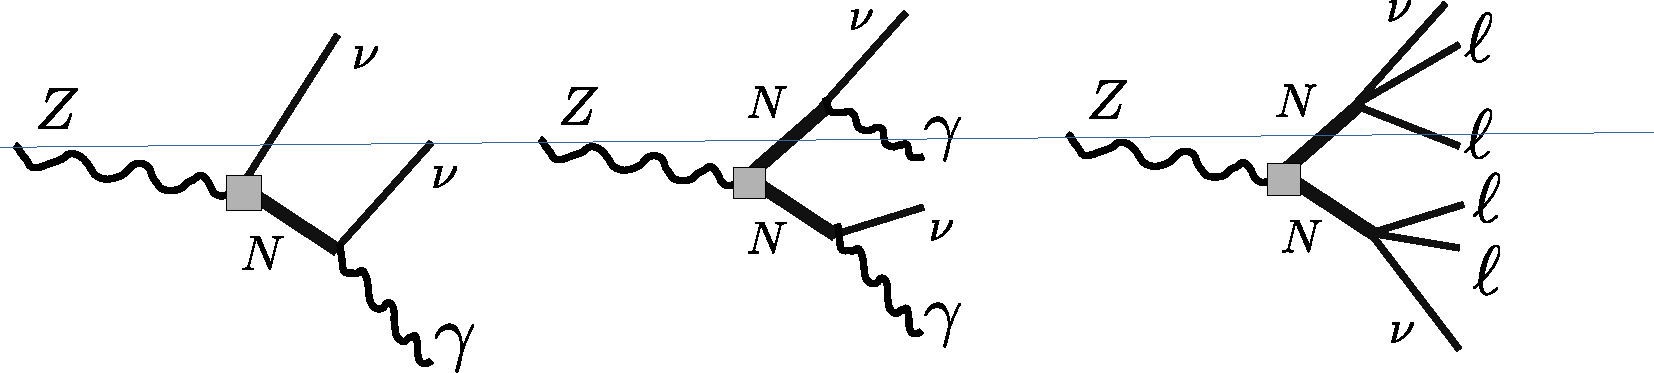
\includegraphics[width=0.82\textwidth]{Figs/rarezdecays-crop.pdf}
  \caption{Rare Z-decay sensitivities as probes of flavour and BSM dynamics. Source: Ref.~\cite{FCCFSRVol1}.}
  \label{fig:rare-z-decays}
\end{figure}
The key lesson is that a projection is meaningful only after the measured observable, the assumptions entering its extraction, and the dominant uncertainty sources have been identified.

Figure~\ref{fig:tau-lfv} is used here as a visual anchor for the surrounding discussion. The important point is not only the numerical projection shown in the figure, but also the way in which the relevant FCC observable is connected to a physical parameter of the Standard Model or to a possible deviation from it.
\begin{figure}[H]
  \centering
  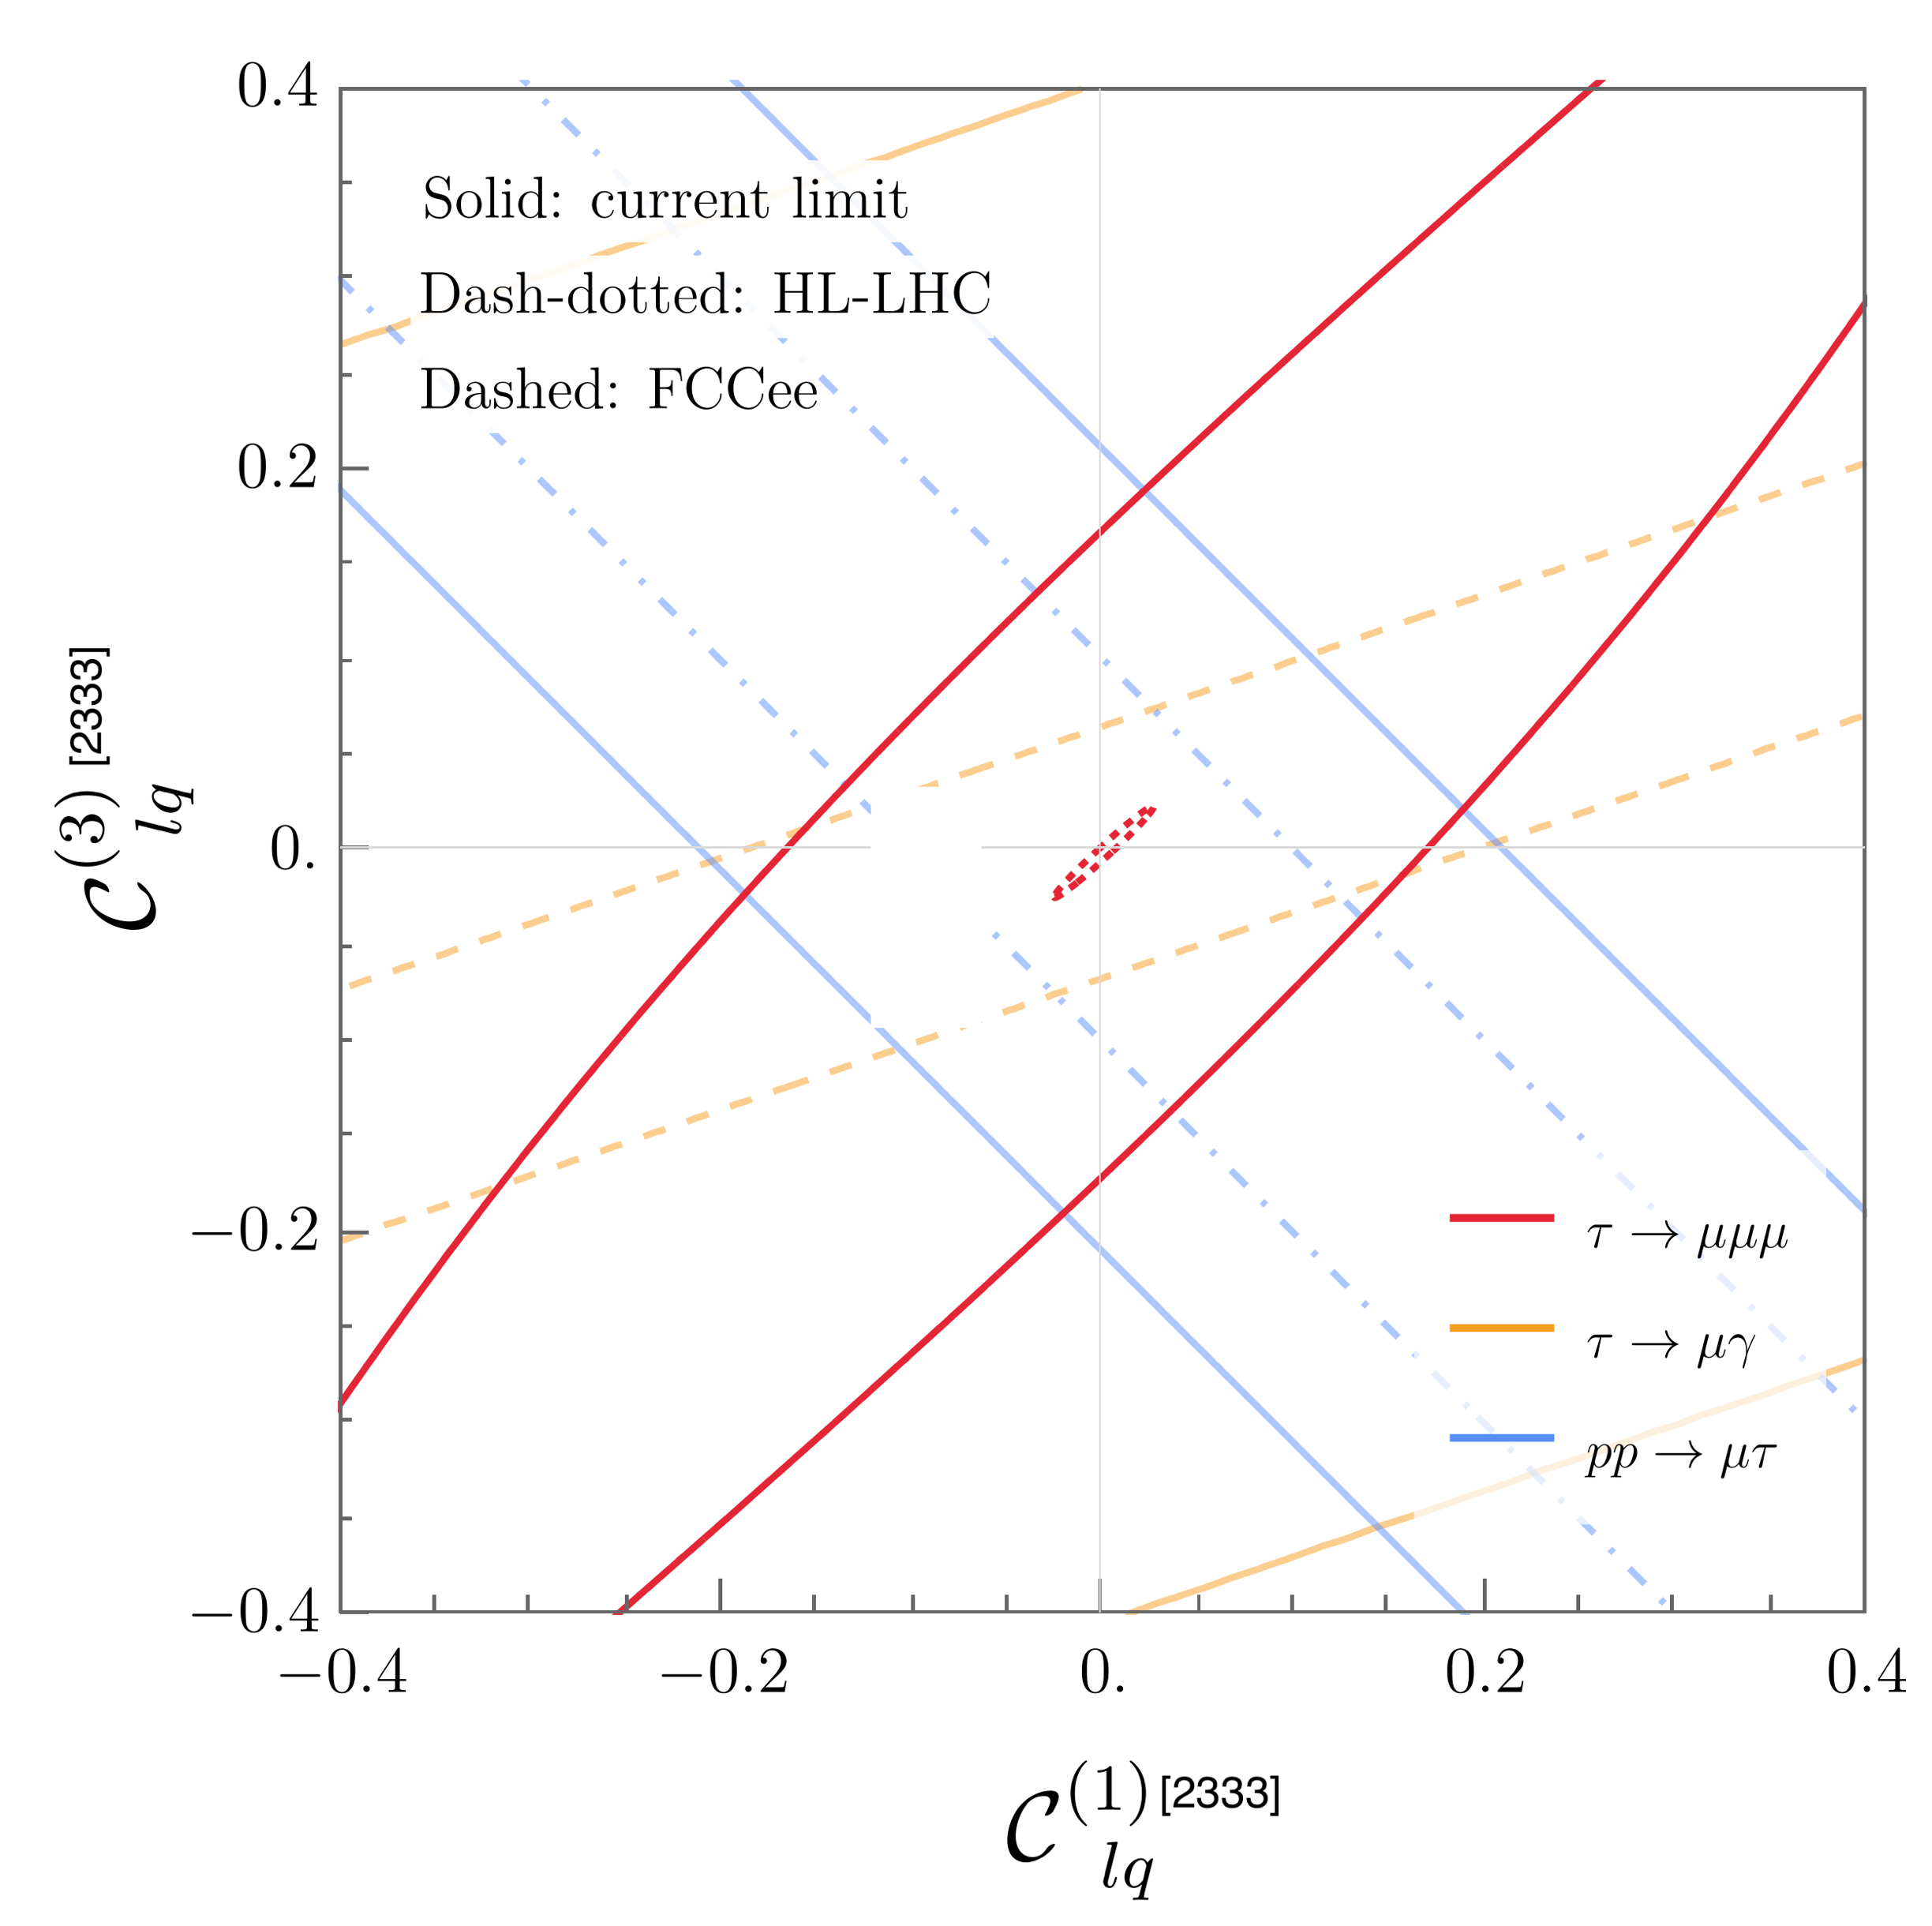
\includegraphics[width=0.82\textwidth]{Figs/Tau_LFV.png}
  \caption{Projected sensitivity to charged-lepton-flavour-violating tau decays at FCC-ee. Source: Ref.~\cite{FCCFSRVol1}.}
  \label{fig:tau-lfv}
\end{figure}
The key lesson is that a projection is meaningful only after the measured observable, the assumptions entering its extraction, and the dominant uncertainty sources have been identified.

Figure~\ref{fig:tau-lfu} is used here as a visual anchor for the surrounding discussion. The important point is not only the numerical projection shown in the figure, but also the way in which the relevant FCC observable is connected to a physical parameter of the Standard Model or to a possible deviation from it.
\begin{figure}[H]
  \centering
  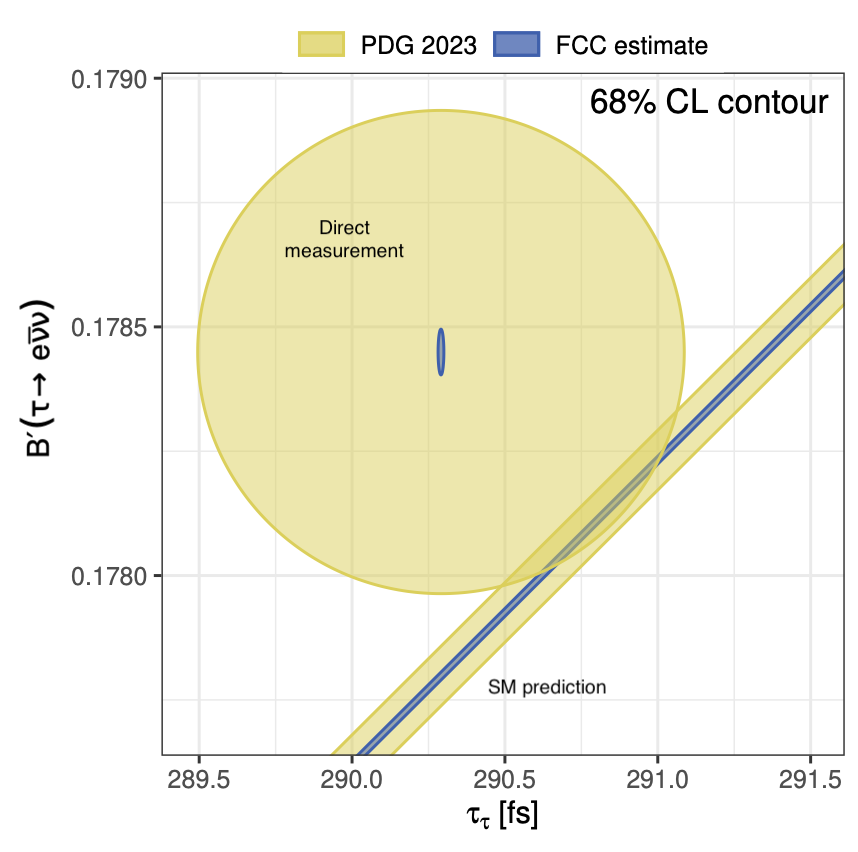
\includegraphics[width=0.82\textwidth]{Figs/tau_LFU_exp.png}
  \caption{Lepton-universality tests in tau observables and the role of high-statistics Z-pole running. Source: Ref.~\cite{DamTau2021}.}
  \label{fig:tau-lfu}
\end{figure}
The key lesson is that a projection is meaningful only after the measured observable, the assumptions entering its extraction, and the dominant uncertainty sources have been identified.

\subsection{Tau physics}
The process
\begin{equation}
  e^+e^-\to Z\to \tau^+\tau^-
\end{equation}
provides a large and clean tau sample. Important observables include the tau lifetime, polarisation, branching fractions, lepton-universality ratios and lepton-flavour-violating decays such as
\begin{equation}
  \tau\to 3\mu,
  \qquad
  \tau\to \mu\gamma,
  \qquad
  \tau\to e\gamma .
\end{equation}
Many BSM scenarios produce enhanced effects in the third generation, making tau physics a natural part of the FCC precision programme rather than a side topic.

\begin{definition}{Lepton universality}{lfu-def}
Lepton universality is the Standard Model property that the electroweak gauge interactions of \(e\), \(\mu\) and \(\tau\) are identical up to mass effects. Ratios of decay rates can test this property with reduced dependence on hadronic uncertainties.
\end{definition}

\begin{examplebox}{Why tau modes are difficult and valuable}{tau-example}
A decay involving tau leptons typically includes one or more neutrinos, making full reconstruction harder than in electron or muon modes. However, the same feature makes tau observables sensitive to interactions that preferentially couple to the third generation. FCC-ee provides a clean environment where the reconstruction challenge can be attacked with high statistics and excellent detector hermeticity.
\end{examplebox}

\begin{guidedchecksbox}
\begin{enumerate}[leftmargin=1.6em]
\item Explain why \(b\to s\nu\bar\nu\) is experimentally difficult but theoretically clean.
\item Give one reason why FCC-ee can be competitive in tau LFV searches despite lower energy than hadron colliders.
\item Identify which detector capabilities are most important for heavy-flavour physics at the Z pole.
\end{enumerate}
\end{guidedchecksbox}

\subsection{Exercises}
\begin{enumerate}[leftmargin=1.6em]
\item Write a short explanation of why rare decays are precision observables.
\item Compare the roles of vertex resolution and particle identification in \(b\)-hadron studies.
\item Explain how lepton-flavour violation differs conceptually from lepton-universality violation.
\end{enumerate}


\newpage
\section{BSM searches enabled by precision and luminosity}
\begin{guidelinebox}
FCC-ee is often described as a precision machine, but precision and direct searches are not separate~\cite{McCulloughBSM2025,AntuschSterile2016,HECATE2021}. The huge Z, W and Higgs samples enable searches for feebly interacting particles, long-lived particles and exotic decays that may be invisible to traditional high-pT searches.
\end{guidelinebox}

\subsection{Heavy neutral leptons}
A minimal extension that addresses neutrino masses introduces heavy neutral leptons \(N\). At the Z pole, a representative process is
\begin{equation}
  Z\to N\nu,
\end{equation}
followed by decays such as
\begin{equation}
  N\to \ell W^*,\qquad N\to \nu Z^*,\qquad N\to \nu H^* .
\end{equation}
The phenomenology depends on the mass of \(N\), its mixing with active neutrinos and its lifetime. Prompt, displaced and detector-stable regimes are all possible.

Figure~\ref{fig:hnl-seesaw} is used here as a visual anchor for the surrounding discussion. The important point is not only the numerical projection shown in the figure, but also the way in which the relevant FCC observable is connected to a physical parameter of the Standard Model or to a possible deviation from it.
\begin{figure}[H]
  \centering
  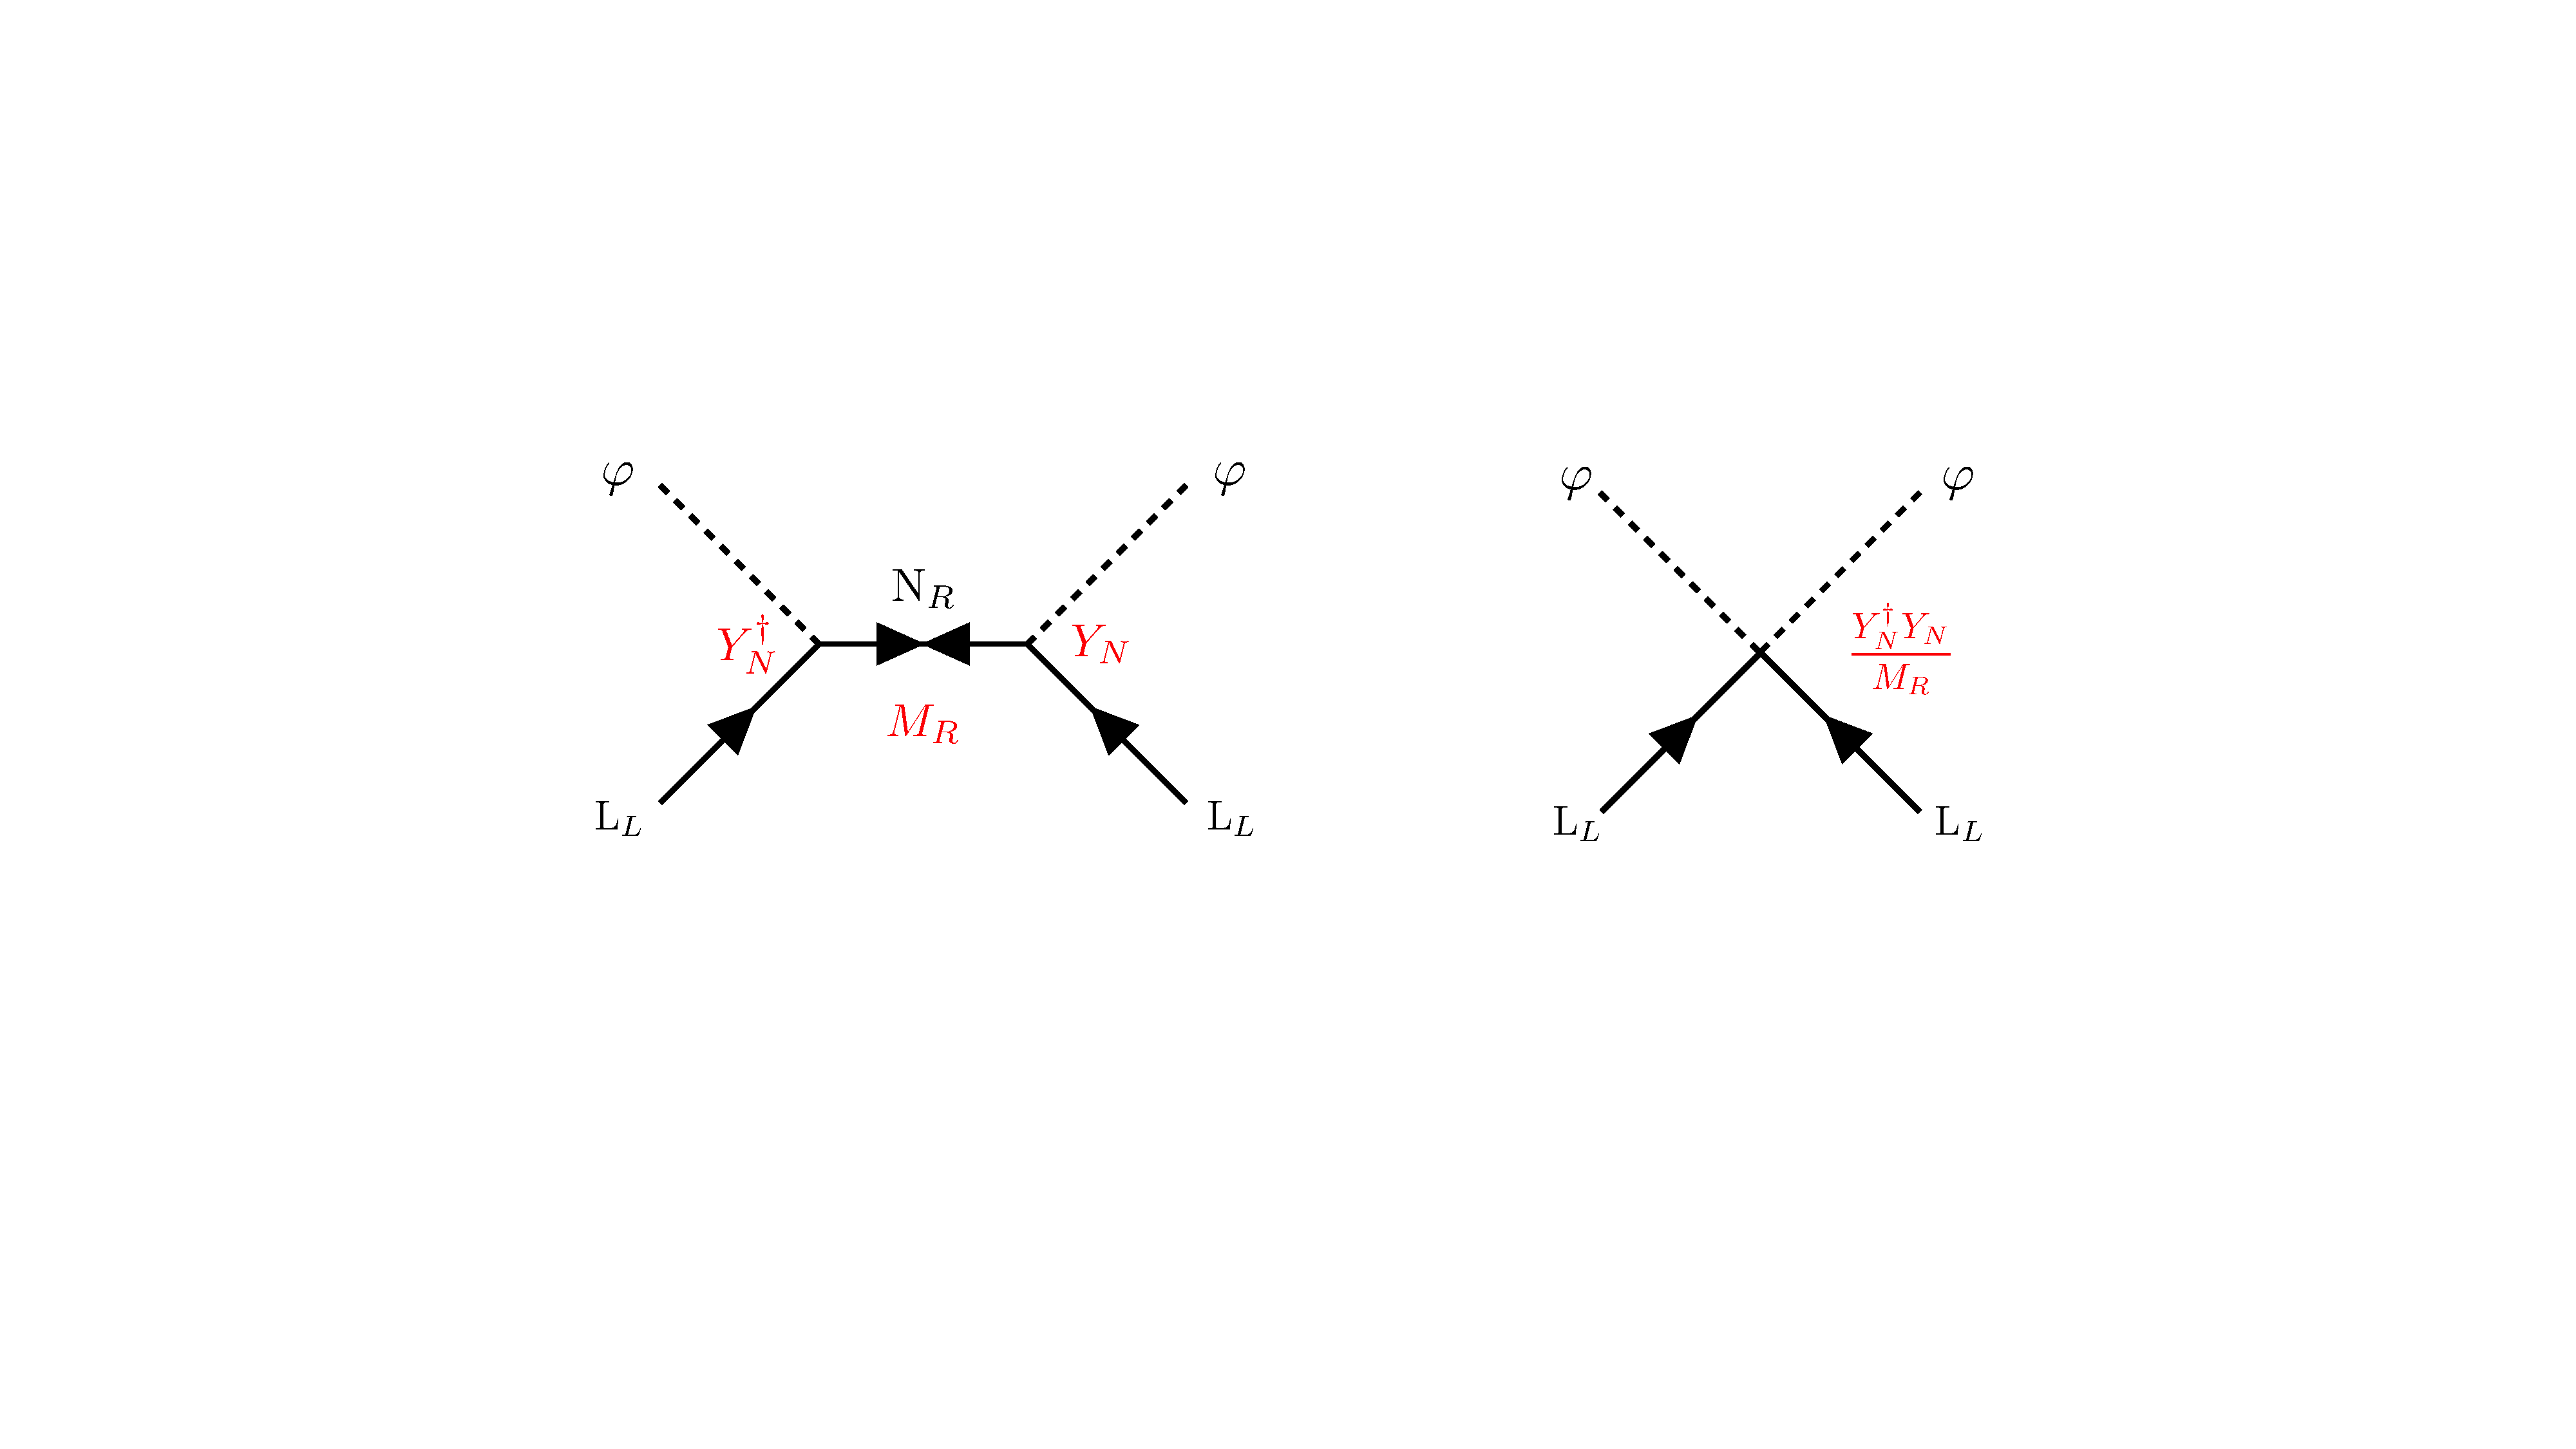
\includegraphics[width=0.86\textwidth]{Figs/TypeISeesaw_FSR.pdf}
  \caption{FCC-ee sensitivity to heavy neutral leptons in type-I seesaw scenarios. Source: Ref.~\cite{FCCFSRVol1}.}
  \label{fig:hnl-seesaw}
\end{figure}
The key lesson is that a projection is meaningful only after the measured observable, the assumptions entering its extraction, and the dominant uncertainty sources have been identified.

\begin{definition}{Long-lived particle}{llp-def}
A long-lived particle is a new state whose decay length is macroscopic on detector scales. Its signature may be a displaced vertex, a displaced lepton or jet, a disappearing track, delayed energy deposition, or missing energy if it decays outside the detector.
\end{definition}

\subsection{Axion-like particles and dark sectors}
Axion-like particles can be produced through processes such as
\begin{equation}
  e^+e^-\to \gamma a,
  \qquad
  a\to \gamma\gamma,\ \ell^+\ell^-,\ \text{hadrons}.
\end{equation}
Dark photons or dark scalars can appear in rare Z or Higgs decays, in radiative return processes, or in displaced signatures. The clean FCC-ee environment is particularly useful when the couplings are too small for high-rate hadron-collider triggers but large enough to yield visible rare decays in enormous samples.

Figure~\ref{fig:alp-sensitivity} is used here as a visual anchor for the surrounding discussion. The important point is not only the numerical projection shown in the figure, but also the way in which the relevant FCC observable is connected to a physical parameter of the Standard Model or to a possible deviation from it.
\begin{figure}[H]
  \centering
  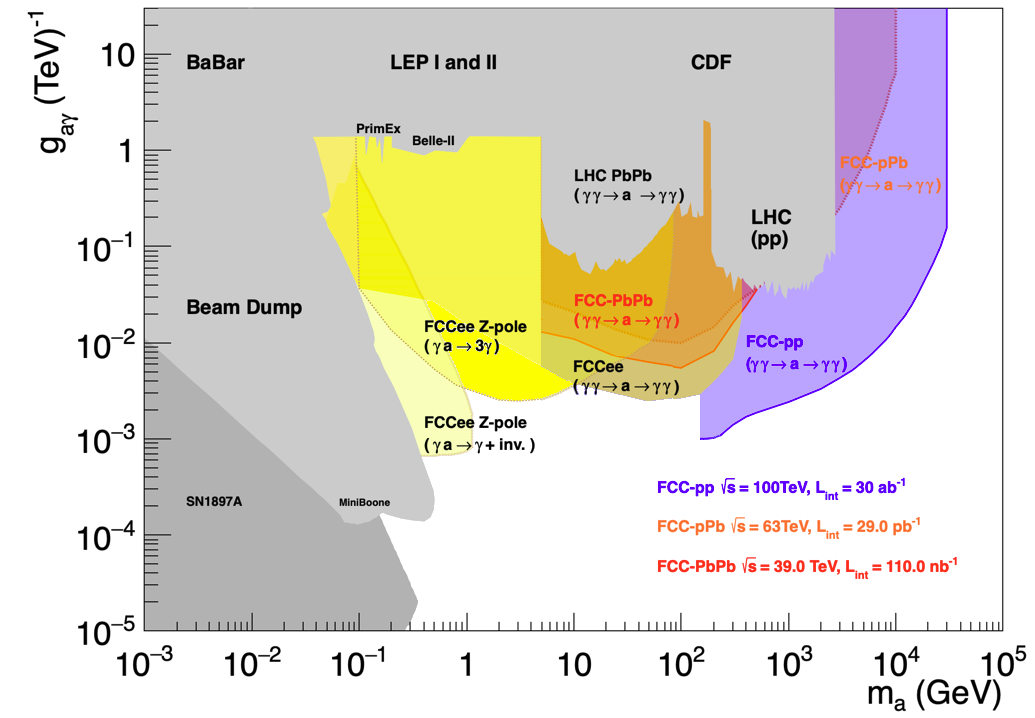
\includegraphics[width=0.86\textwidth]{Figs/alp_final_FCCeehh_col_FSR.png}
  \caption{Sensitivity to axion-like particles across FCC-ee and FCC-hh channels. Source: Ref.~\cite{FCCFSRVol1}.}
  \label{fig:alp-sensitivity}
\end{figure}
The key lesson is that a projection is meaningful only after the measured observable, the assumptions entering its extraction, and the dominant uncertainty sources have been identified.

Figure~\ref{fig:llp-lines} is used here as a visual anchor for the surrounding discussion. The important point is not only the numerical projection shown in the figure, but also the way in which the relevant FCC observable is connected to a physical parameter of the Standard Model or to a possible deviation from it.
\begin{figure}[H]
  \centering
  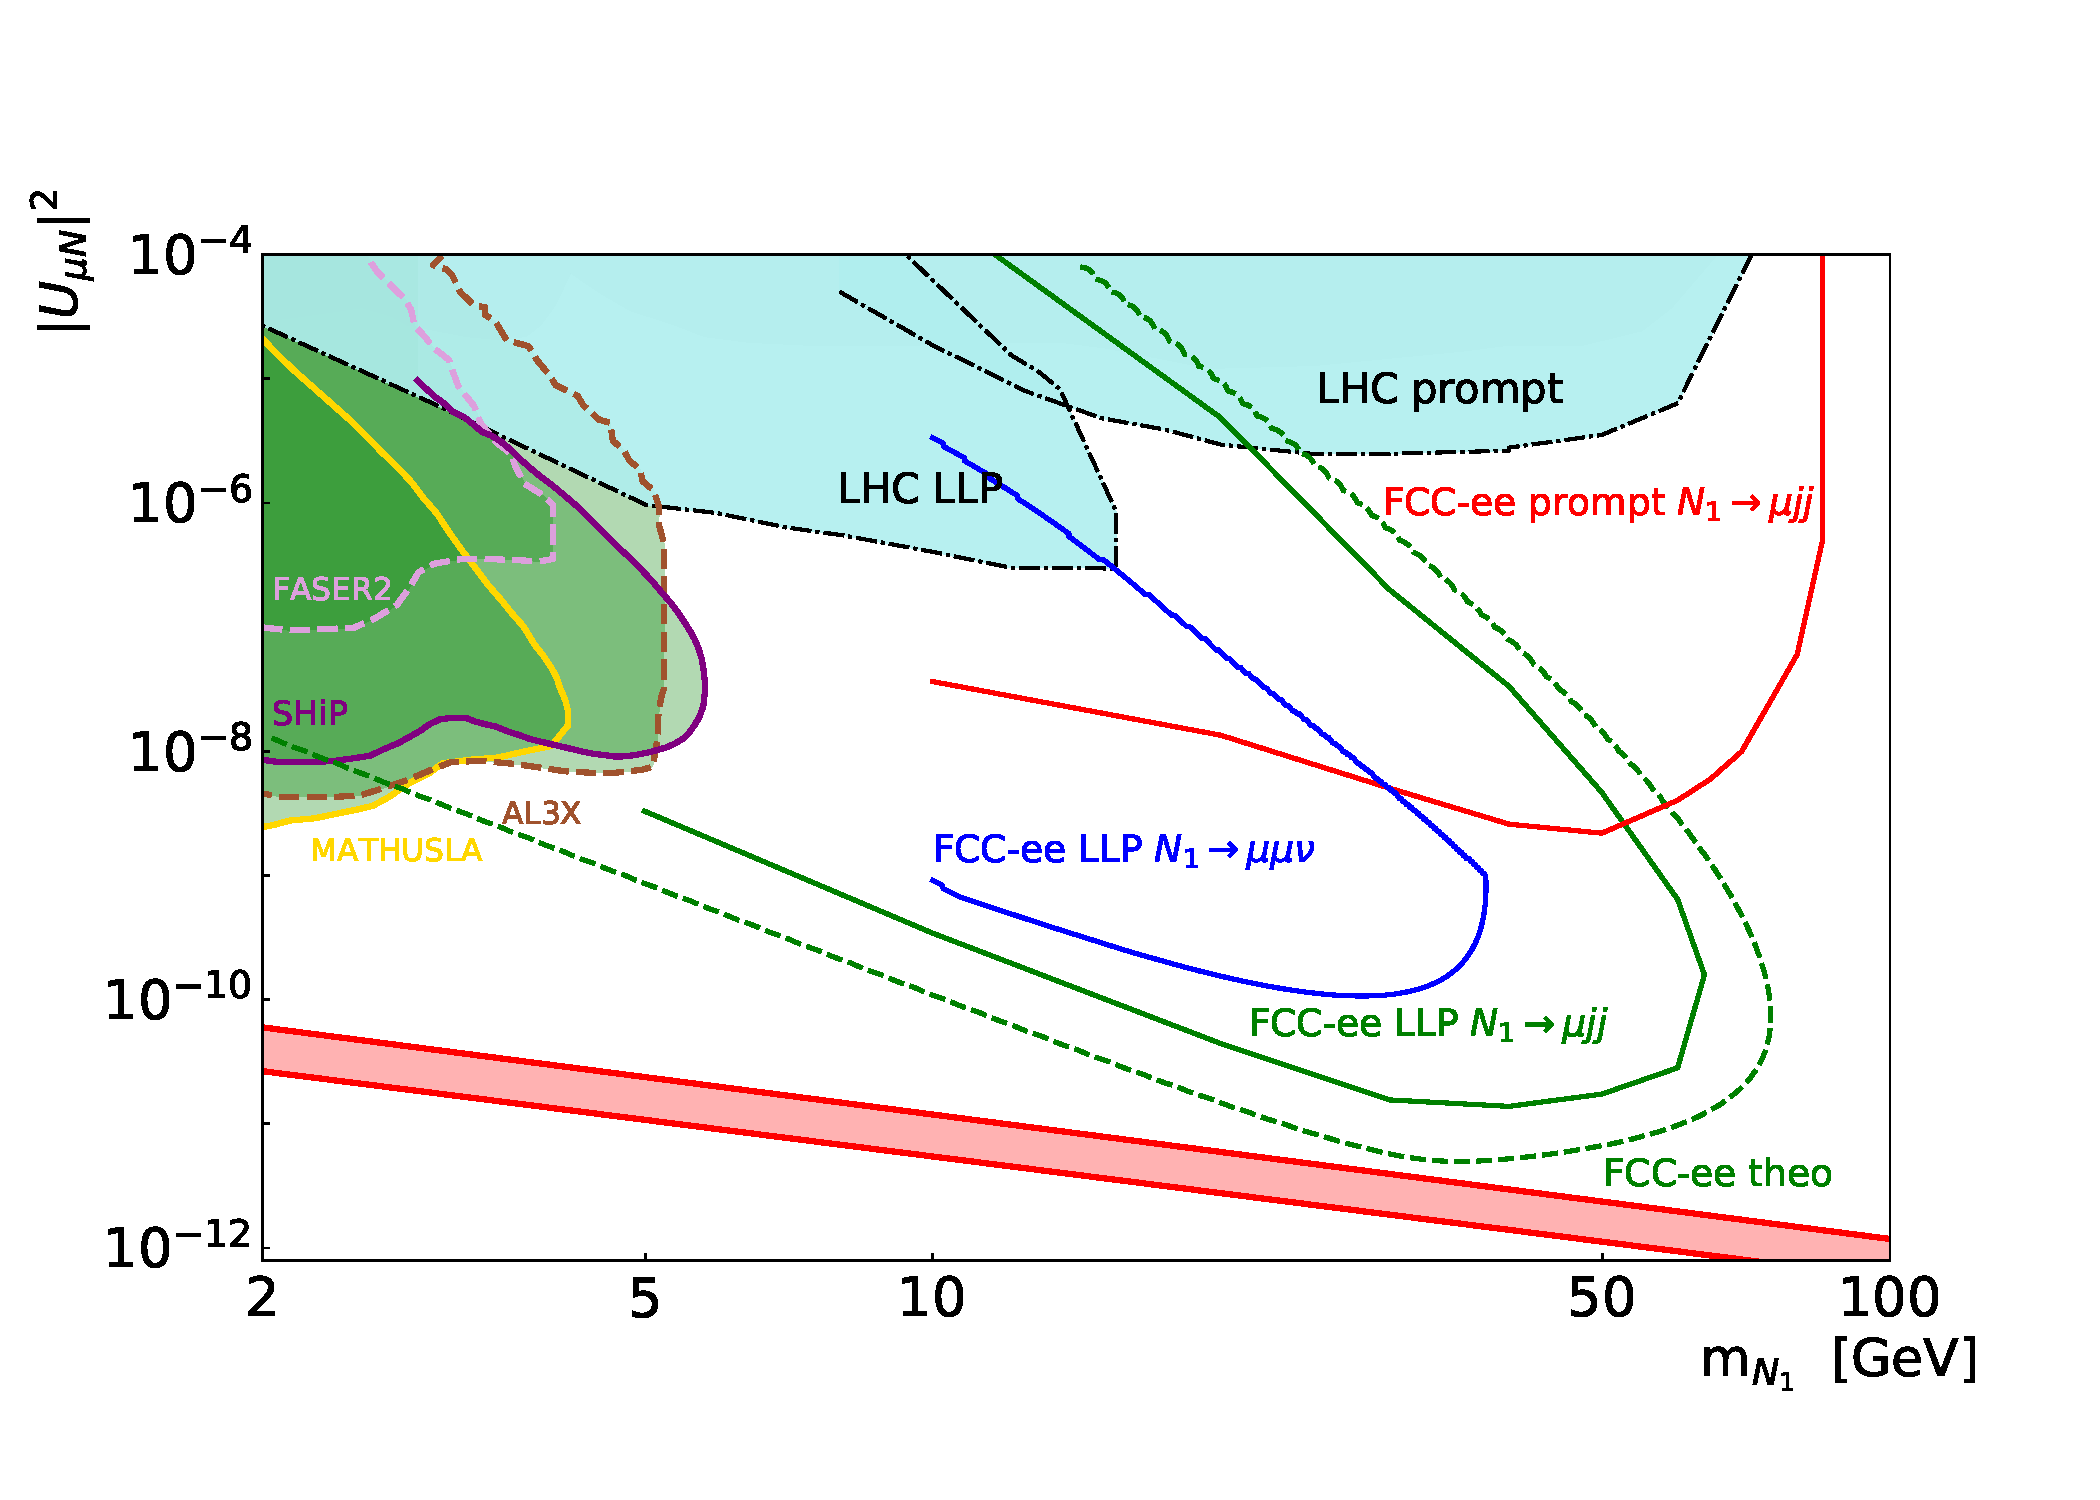
\includegraphics[width=0.86\textwidth]{Figs/fcc_lines_LLP_FSR.pdf}
  \caption{Long-lived-particle sensitivity in representative FCC scenarios. Source: Ref.~\cite{FCCFSRVol1}.}
  \label{fig:llp-lines}
\end{figure}
The key lesson is that a projection is meaningful only after the measured observable, the assumptions entering its extraction, and the dominant uncertainty sources have been identified.

\subsection{Exotic Higgs decays}
The Higgs can act as a portal to a hidden sector. A representative topology is
\begin{equation}
  H\to SS,
  \qquad
  S\to b\bar b,\ \tau^+\tau^-,\ gg,\ \text{invisible},\ \text{or displaced final states}.
\end{equation}
The recoil method is again crucial: exotic or invisible Higgs decays do not prevent the inclusive \(ZH\) process from being counted. This gives FCC-ee a robust handle on non-standard Higgs branching fractions.

Figure~\ref{fig:exotic-higgs-llp} is used here as a visual anchor for the surrounding discussion. The important point is not only the numerical projection shown in the figure, but also the way in which the relevant FCC observable is connected to a physical parameter of the Standard Model or to a possible deviation from it.
\begin{figure}[H]
  \centering
  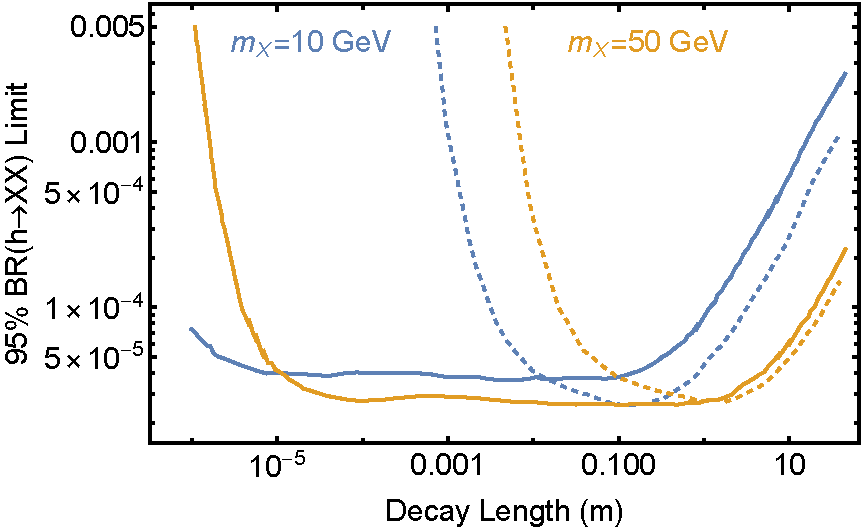
\includegraphics[width=0.86\textwidth]{Figs/ExoticHiggsLLP_FSR.pdf}
  \caption{Projected sensitivity to exotic Higgs decays with long-lived particles. Source: Ref.~\cite{FCCFSRVol1}.}
  \label{fig:exotic-higgs-llp}
\end{figure}
The key lesson is that a projection is meaningful only after the measured observable, the assumptions entering its extraction, and the dominant uncertainty sources have been identified.

Figure~\ref{fig:h2ss-diagram} is used here as a visual anchor for the surrounding discussion. The important point is not only the numerical projection shown in the figure, but also the way in which the relevant FCC observable is connected to a physical parameter of the Standard Model or to a possible deviation from it.
\begin{figure}[H]
  \centering
  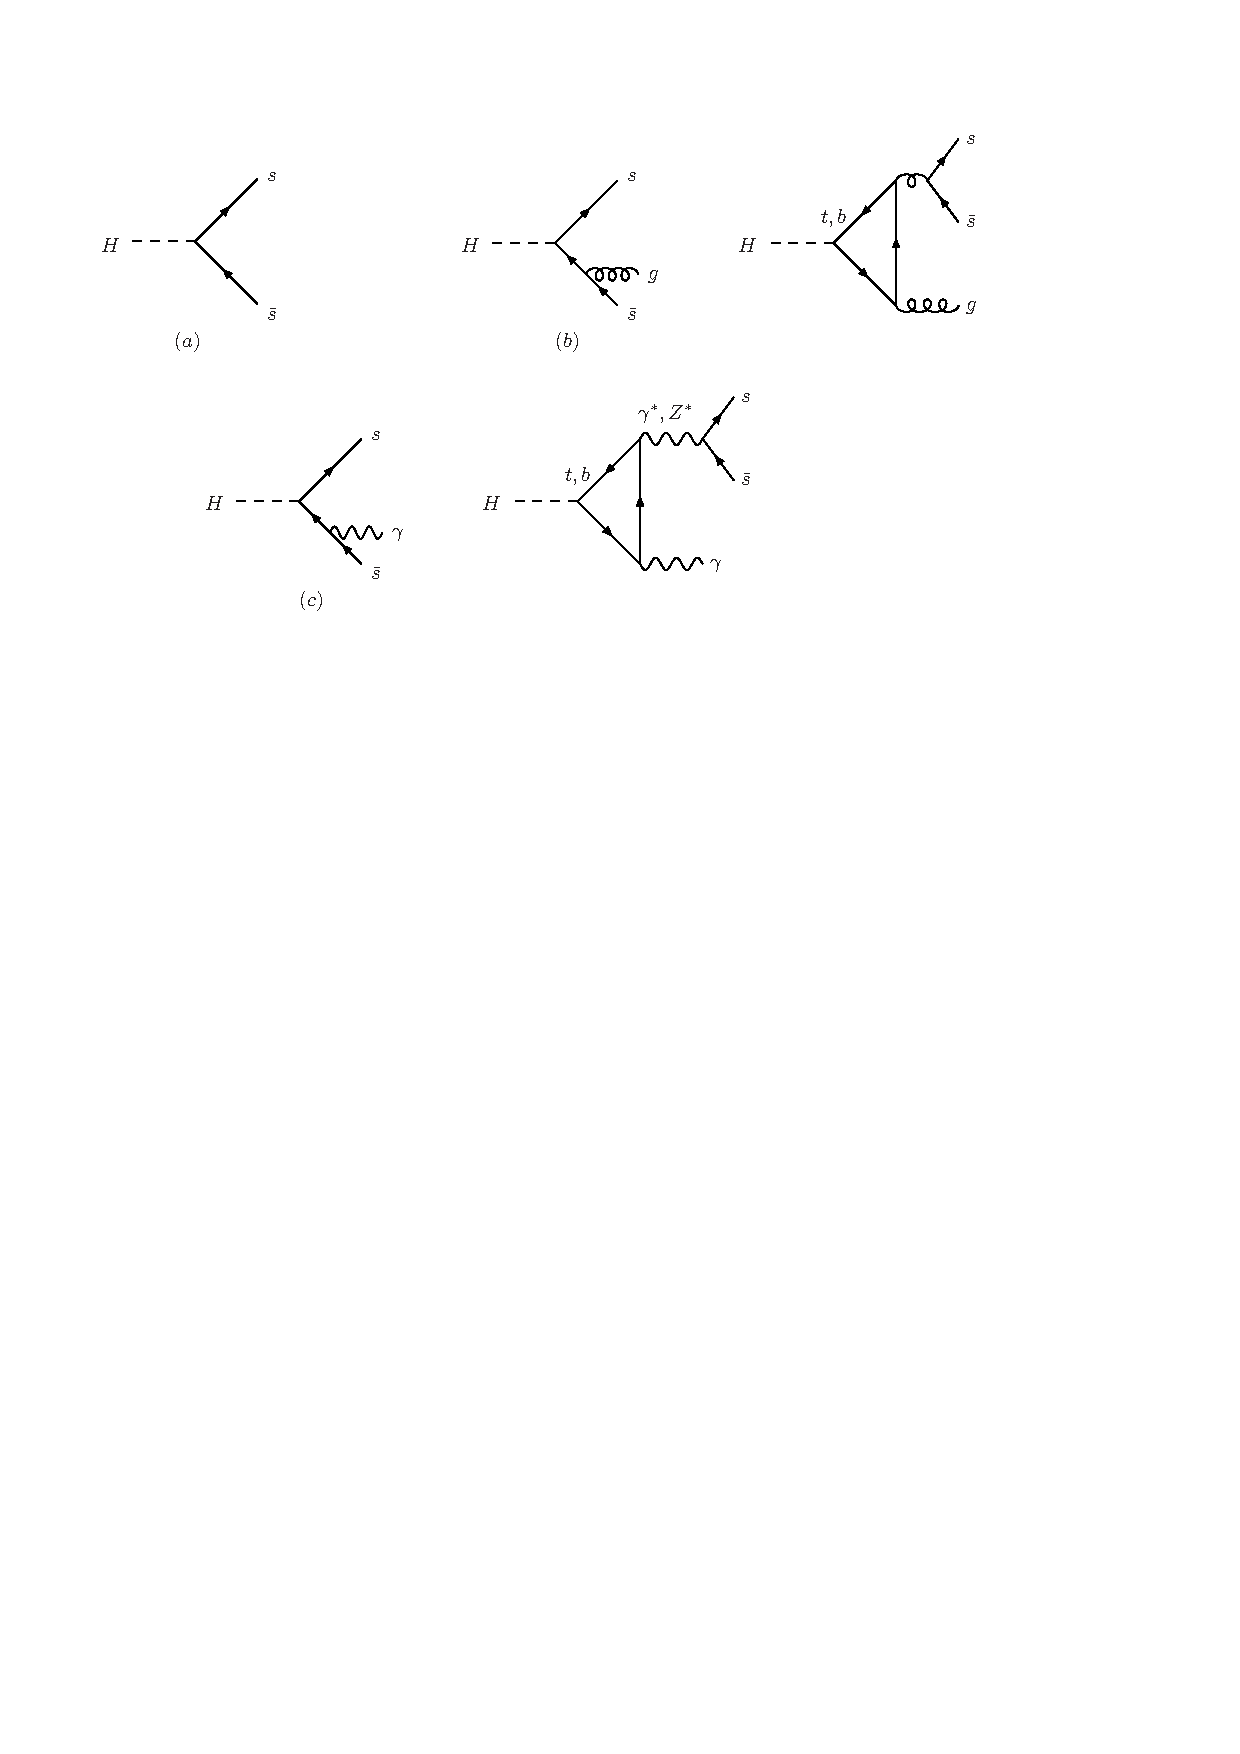
\includegraphics[width=0.70\textwidth]{Figs/HtoSS/h2ss_dia.pdf}
  \caption{Higgs-portal topology \(H\to SS\), with light scalars decaying to visible or invisible final states. Source: Ref.~\cite{ECFAFactories2025}.}
  \label{fig:h2ss-diagram}
\end{figure}
The key lesson is that a projection is meaningful only after the measured observable, the assumptions entering its extraction, and the dominant uncertainty sources have been identified.

Figure~\ref{fig:h2ss-weak} is used here as a visual anchor for the surrounding discussion. The important point is not only the numerical projection shown in the figure, but also the way in which the relevant FCC observable is connected to a physical parameter of the Standard Model or to a possible deviation from it.
\begin{figure}[H]
  \centering
  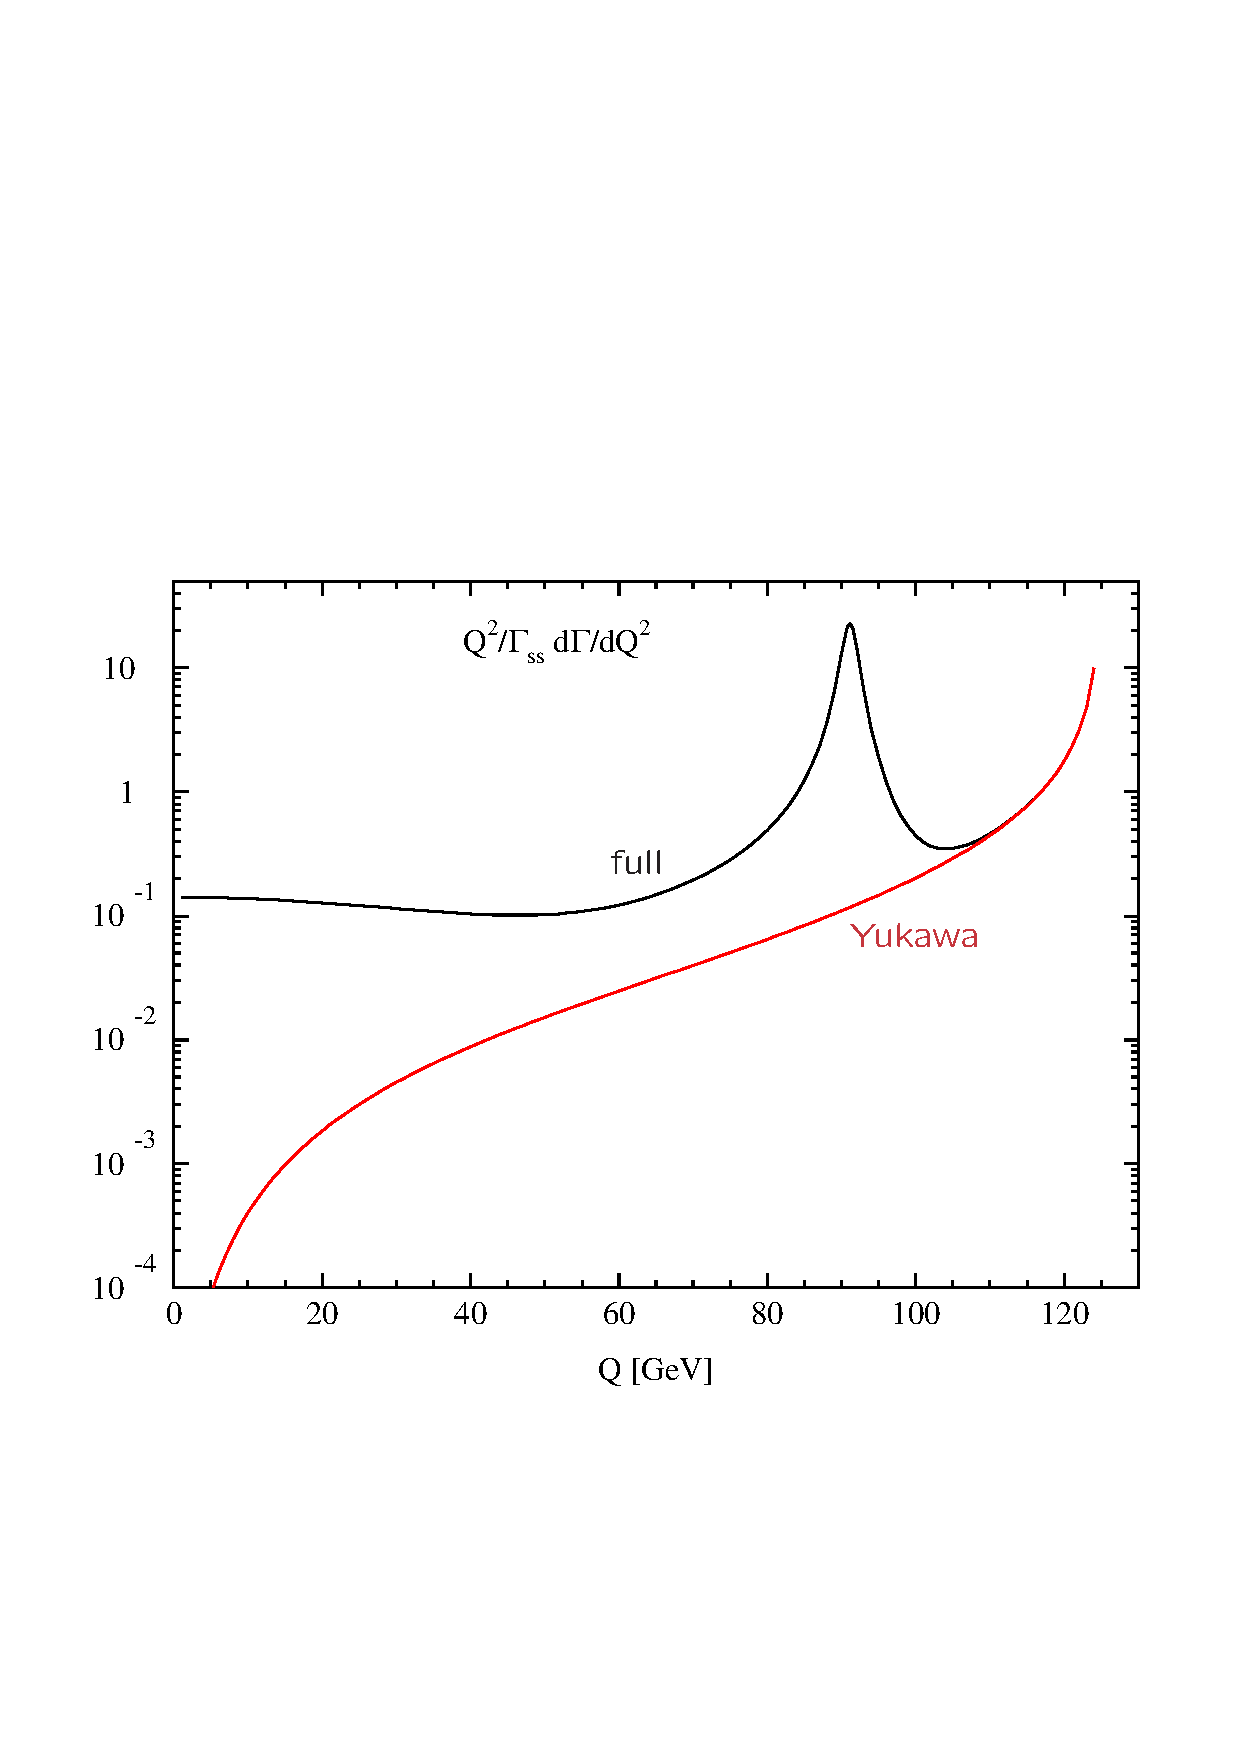
\includegraphics[width=0.82\textwidth]{Figs/HtoSS/h2ss_weak.pdf}
  \caption{Example weakly coupled Higgs-portal sensitivity in exotic Higgs decays. Source: Ref.~\cite{ECFAFactories2025}.}
  \label{fig:h2ss-weak}
\end{figure}
The key lesson is that a projection is meaningful only after the measured observable, the assumptions entering its extraction, and the dominant uncertainty sources have been identified.

\begin{examplebox}{Prompt versus displaced exotic Higgs decays}{prompt-displaced}
If \(S\) decays promptly, the analysis may resemble a multi-jet or multi-lepton resonance search inside a Higgs event. If \(S\) is long lived, the event may contain displaced vertices or tracks that do not point back to the interaction point. The same underlying decay \(H\to SS\) therefore maps to very different detector requirements depending on the lifetime.
\end{examplebox}

\begin{guidedchecksbox}
\begin{enumerate}[leftmargin=1.6em]
\item Why is \(Z\to N\nu\) especially interesting at a Tera-Z machine?
\item Explain why the recoil method is useful for invisible Higgs decays.
\item List three detector signatures of long-lived particles.
\end{enumerate}
\end{guidedchecksbox}

\subsection{Exercises}
\begin{enumerate}[leftmargin=1.6em]
\item Draw the topology for \(Z\to N\nu\) followed by \(N\to \ell jj\).
\item Explain how the sensitivity to a long-lived particle depends on detector radius and vertex resolution.
\item Compare exotic Z decays and exotic Higgs decays as BSM search channels at FCC-ee.
\end{enumerate}


\newpage
\section{Theory precision requirements}
\begin{guidelinebox}
FCC-ee precision can be limited by theory rather than by event counts. This chapter reviews the main theoretical ingredients: electroweak higher orders, QED radiation, QCD corrections, luminosity theory, hadronic vacuum polarisation, Monte Carlo modelling and parametric uncertainties.
\end{guidelinebox}

\subsection{The precision budget}
A useful decomposition is
\begin{equation}
  \delta_{\rm tot}^2=\delta_{\rm stat}^2+\delta_{\rm syst}^2+\delta_{\rm th}^2+\delta_{\rm param}^2 .
  \label{eq:uncert-budget}
\end{equation}
At FCC-ee, \(\delta_{\rm stat}\) can become extremely small. The limiting terms may therefore be theoretical missing higher orders, input-parameter uncertainties, beam-energy modelling, luminosity theory, or non-perturbative effects.

Figure~\ref{fig:vacuum-polarization} is used here as a visual anchor for the surrounding discussion. The important point is not only the numerical projection shown in the figure, but also the way in which the relevant FCC observable is connected to a physical parameter of the Standard Model or to a possible deviation from it.
\begin{figure}[H]
  \centering
  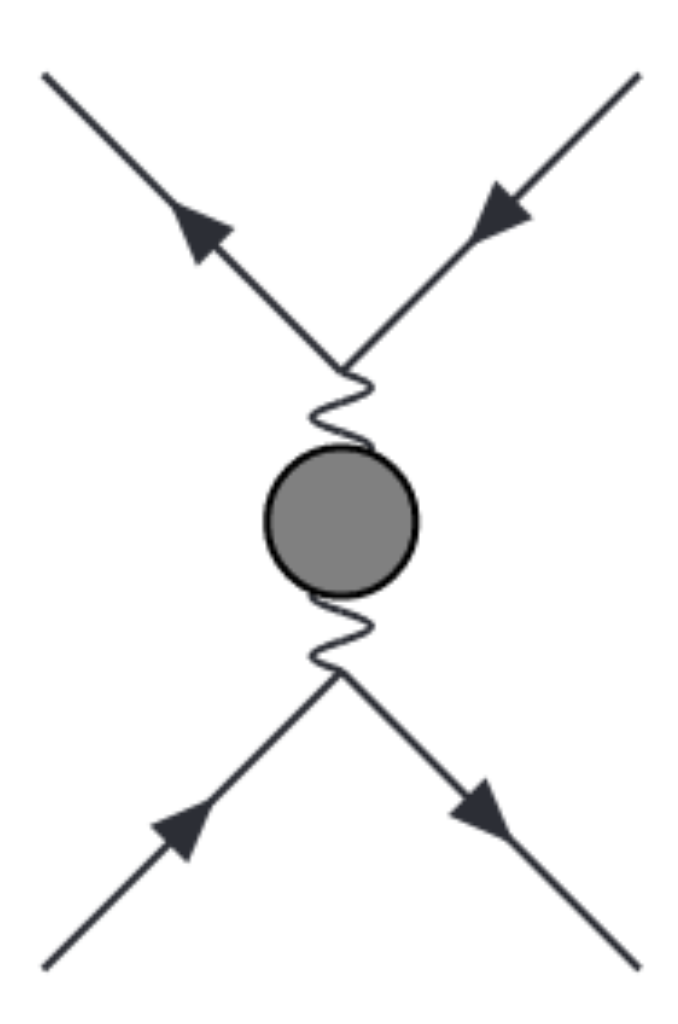
\includegraphics[width=0.58\textwidth]{Figs/VacuumPolarization.png}
  \caption{Vacuum-polarisation correction entering precision electroweak inputs and luminosity theory. Source: Ref.~\cite{ECFAFactories2025}.}
  \label{fig:vacuum-polarization}
\end{figure}
The key lesson is that a projection is meaningful only after the measured observable, the assumptions entering its extraction, and the dominant uncertainty sources have been identified.

Figure~\ref{fig:light-by-light} is used here as a visual anchor for the surrounding discussion. The important point is not only the numerical projection shown in the figure, but also the way in which the relevant FCC observable is connected to a physical parameter of the Standard Model or to a possible deviation from it.
\begin{figure}[H]
  \centering
  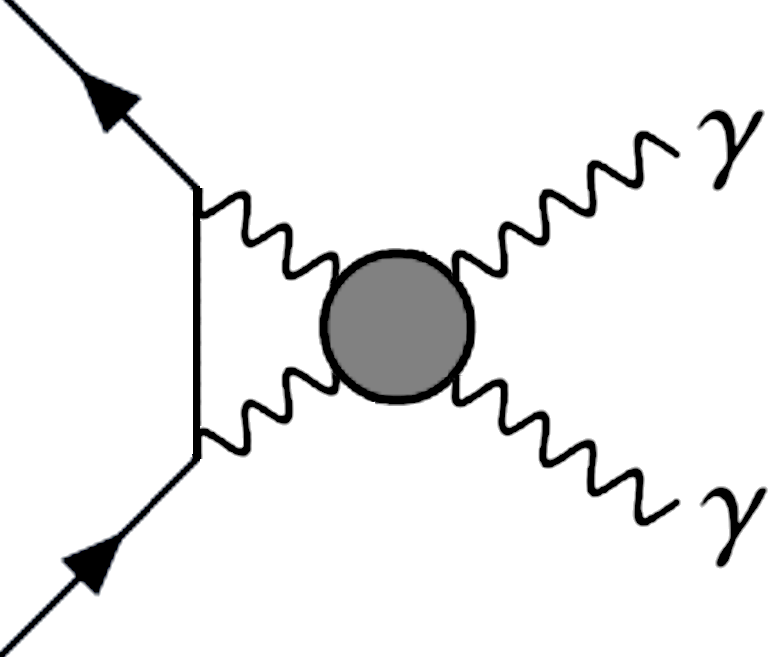
\includegraphics[width=0.58\textwidth]{Figs/LbL_diphoton_diag.png}
  \caption{Light-by-light contribution relevant for precision QED and photon final states. Source: Ref.~\cite{ECFAFactories2025}.}
  \label{fig:light-by-light}
\end{figure}
The key lesson is that a projection is meaningful only after the measured observable, the assumptions entering its extraction, and the dominant uncertainty sources have been identified.

Figure~\ref{fig:gamma-gamma-lbl} is used here as a visual anchor for the surrounding discussion. The important point is not only the numerical projection shown in the figure, but also the way in which the relevant FCC observable is connected to a physical parameter of the Standard Model or to a possible deviation from it.
\begin{figure}[H]
  \centering
  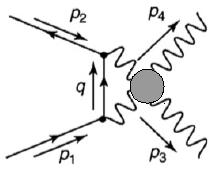
\includegraphics[width=0.58\textwidth]{Figs/gg_lbl.png}
  \caption{Representative photon-induced light-by-light topology in precision calculations. Source: Ref.~\cite{ECFAFactories2025}.}
  \label{fig:gamma-gamma-lbl}
\end{figure}
The key lesson is that a projection is meaningful only after the measured observable, the assumptions entering its extraction, and the dominant uncertainty sources have been identified.

\subsection{Running electromagnetic coupling}
The effective electromagnetic coupling at momentum transfer \(q^2\) can be written as
\begin{equation}
  \alpha(q^2)=\frac{\alpha(0)}{1-\Delta\alpha(q^2)} ,
\end{equation}
with
\begin{equation}
  \Delta\alpha(q^2)=\Delta\alpha_{\rm lep}(q^2)+\Delta\alpha_{\rm had}^{(5)}(q^2)+\Delta\alpha_{\rm top}(q^2) .
\end{equation}
The hadronic contribution is a major parametric input to electroweak fits. FCC-ee can both benefit from and contribute to improved determinations of \(\alpha_{\rm QED}(m_Z^2)\).

\begin{definition}{Parametric uncertainty}{parametric-uncertainty}
A parametric uncertainty is the uncertainty induced in a prediction by imperfect knowledge of an input parameter such as \(m_t\), \(m_H\), \(\alpha_s(m_Z)\), \(\alpha_{\rm QED}(m_Z)\), or quark masses. It is distinct from missing higher-order uncertainty, although the two can interact in global fits.
\end{definition}

\subsection{QCD and non-perturbative effects}
QCD enters FCC-ee precision in many places: hadronic Z and W decays, event shapes, jet rates, flavour tagging, Higgs decays to gluons and heavy quarks, top-threshold calculations, and hadronisation uncertainties. The strong coupling can be extracted from several observables, but the interpretation requires careful control of perturbative orders, hadronisation corrections and correlations.
\begin{equation}
  R_Z = \frac{\Gamma(Z\to \text{hadrons})}{\Gamma(Z\to \ell^+\ell^-)}
  = R_Z^{(0)}\left[1+c_1\frac{\alpha_s}{\pi}+c_2\left(\frac{\alpha_s}{\pi}\right)^2+\cdots\right] .
\end{equation}

\subsection{Monte Carlo generators and radiation}
Initial-state radiation changes the effective collision energy event by event. Beamstrahlung and beam-energy spread further smear threshold observables. Final-state radiation, parton showers and hadronisation affect reconstructed masses, jet observables and flavour-tagging templates. A precision lecture note should therefore treat event generators not as black boxes, but as theory tools with assumptions and uncertainties.

\begin{remarkbox}{Theory precision is part of the experimental design}{theory-design}
If a projected measurement is more precise than the available theory prediction, the quoted experimental uncertainty does not by itself define the physics reach. The theory-improvement programme is therefore part of the FCC physics case, not a later optional refinement.
\end{remarkbox}

\begin{guidedchecksbox}
\begin{enumerate}[leftmargin=1.6em]
\item Identify one FCC-ee observable limited mainly by beam-energy calibration and one limited mainly by QCD modelling.
\item Explain why hadronic vacuum polarisation affects electroweak precision tests.
\item Give an example where a Monte Carlo modelling uncertainty could bias a coupling extraction.
\end{enumerate}
\end{guidedchecksbox}

\subsection{Exercises}
\begin{enumerate}[leftmargin=1.6em]
\item Use Eq.~\eqref{eq:uncert-budget} to discuss a case where reducing statistics does not improve the final precision.
\item Explain why ISR must be included in the top-threshold line-shape prediction.
\item Discuss how measurements at the Z pole can improve QCD knowledge used in Higgs and top analyses.
\end{enumerate}


\newpage
\section{Detector and reconstruction requirements}
\begin{guidelinebox}
The detector is part of the precision argument, with requirements studied for FCC-ee detector concepts and common software frameworks~\cite{DamDetector2025,IDEA2025,AzziPerez2021,Key4hep2022}. Vertexing, tracking, calorimetry, particle identification, timing and software all determine whether the theoretical reach of FCC-ee can be realised experimentally.
\end{guidelinebox}

\subsection{From physics goals to detector requirements}
The same detector must support several distinct tasks: reconstructing \(Z\) bosons for Higgs recoil, separating \(H\to b\bar b\), \(H\to c\bar c\) and \(H\to gg\), measuring tau polarisation and lifetime, identifying displaced vertices from LLPs, and controlling the momentum scale for precision electroweak observables. Representative processes include
\begin{equation}
  H\to b\bar b,\quad H\to c\bar c,\quad Z\to b\bar b,
  \quad \tau\to X\nu,\quad e^+e^-\to ZH.
\end{equation}

Figure~\ref{fig:cld-view} is used here as a visual anchor for the surrounding discussion. The important point is not only the numerical projection shown in the figure, but also the way in which the relevant FCC observable is connected to a physical parameter of the Standard Model or to a possible deviation from it.
\begin{figure}[H]
  \centering
  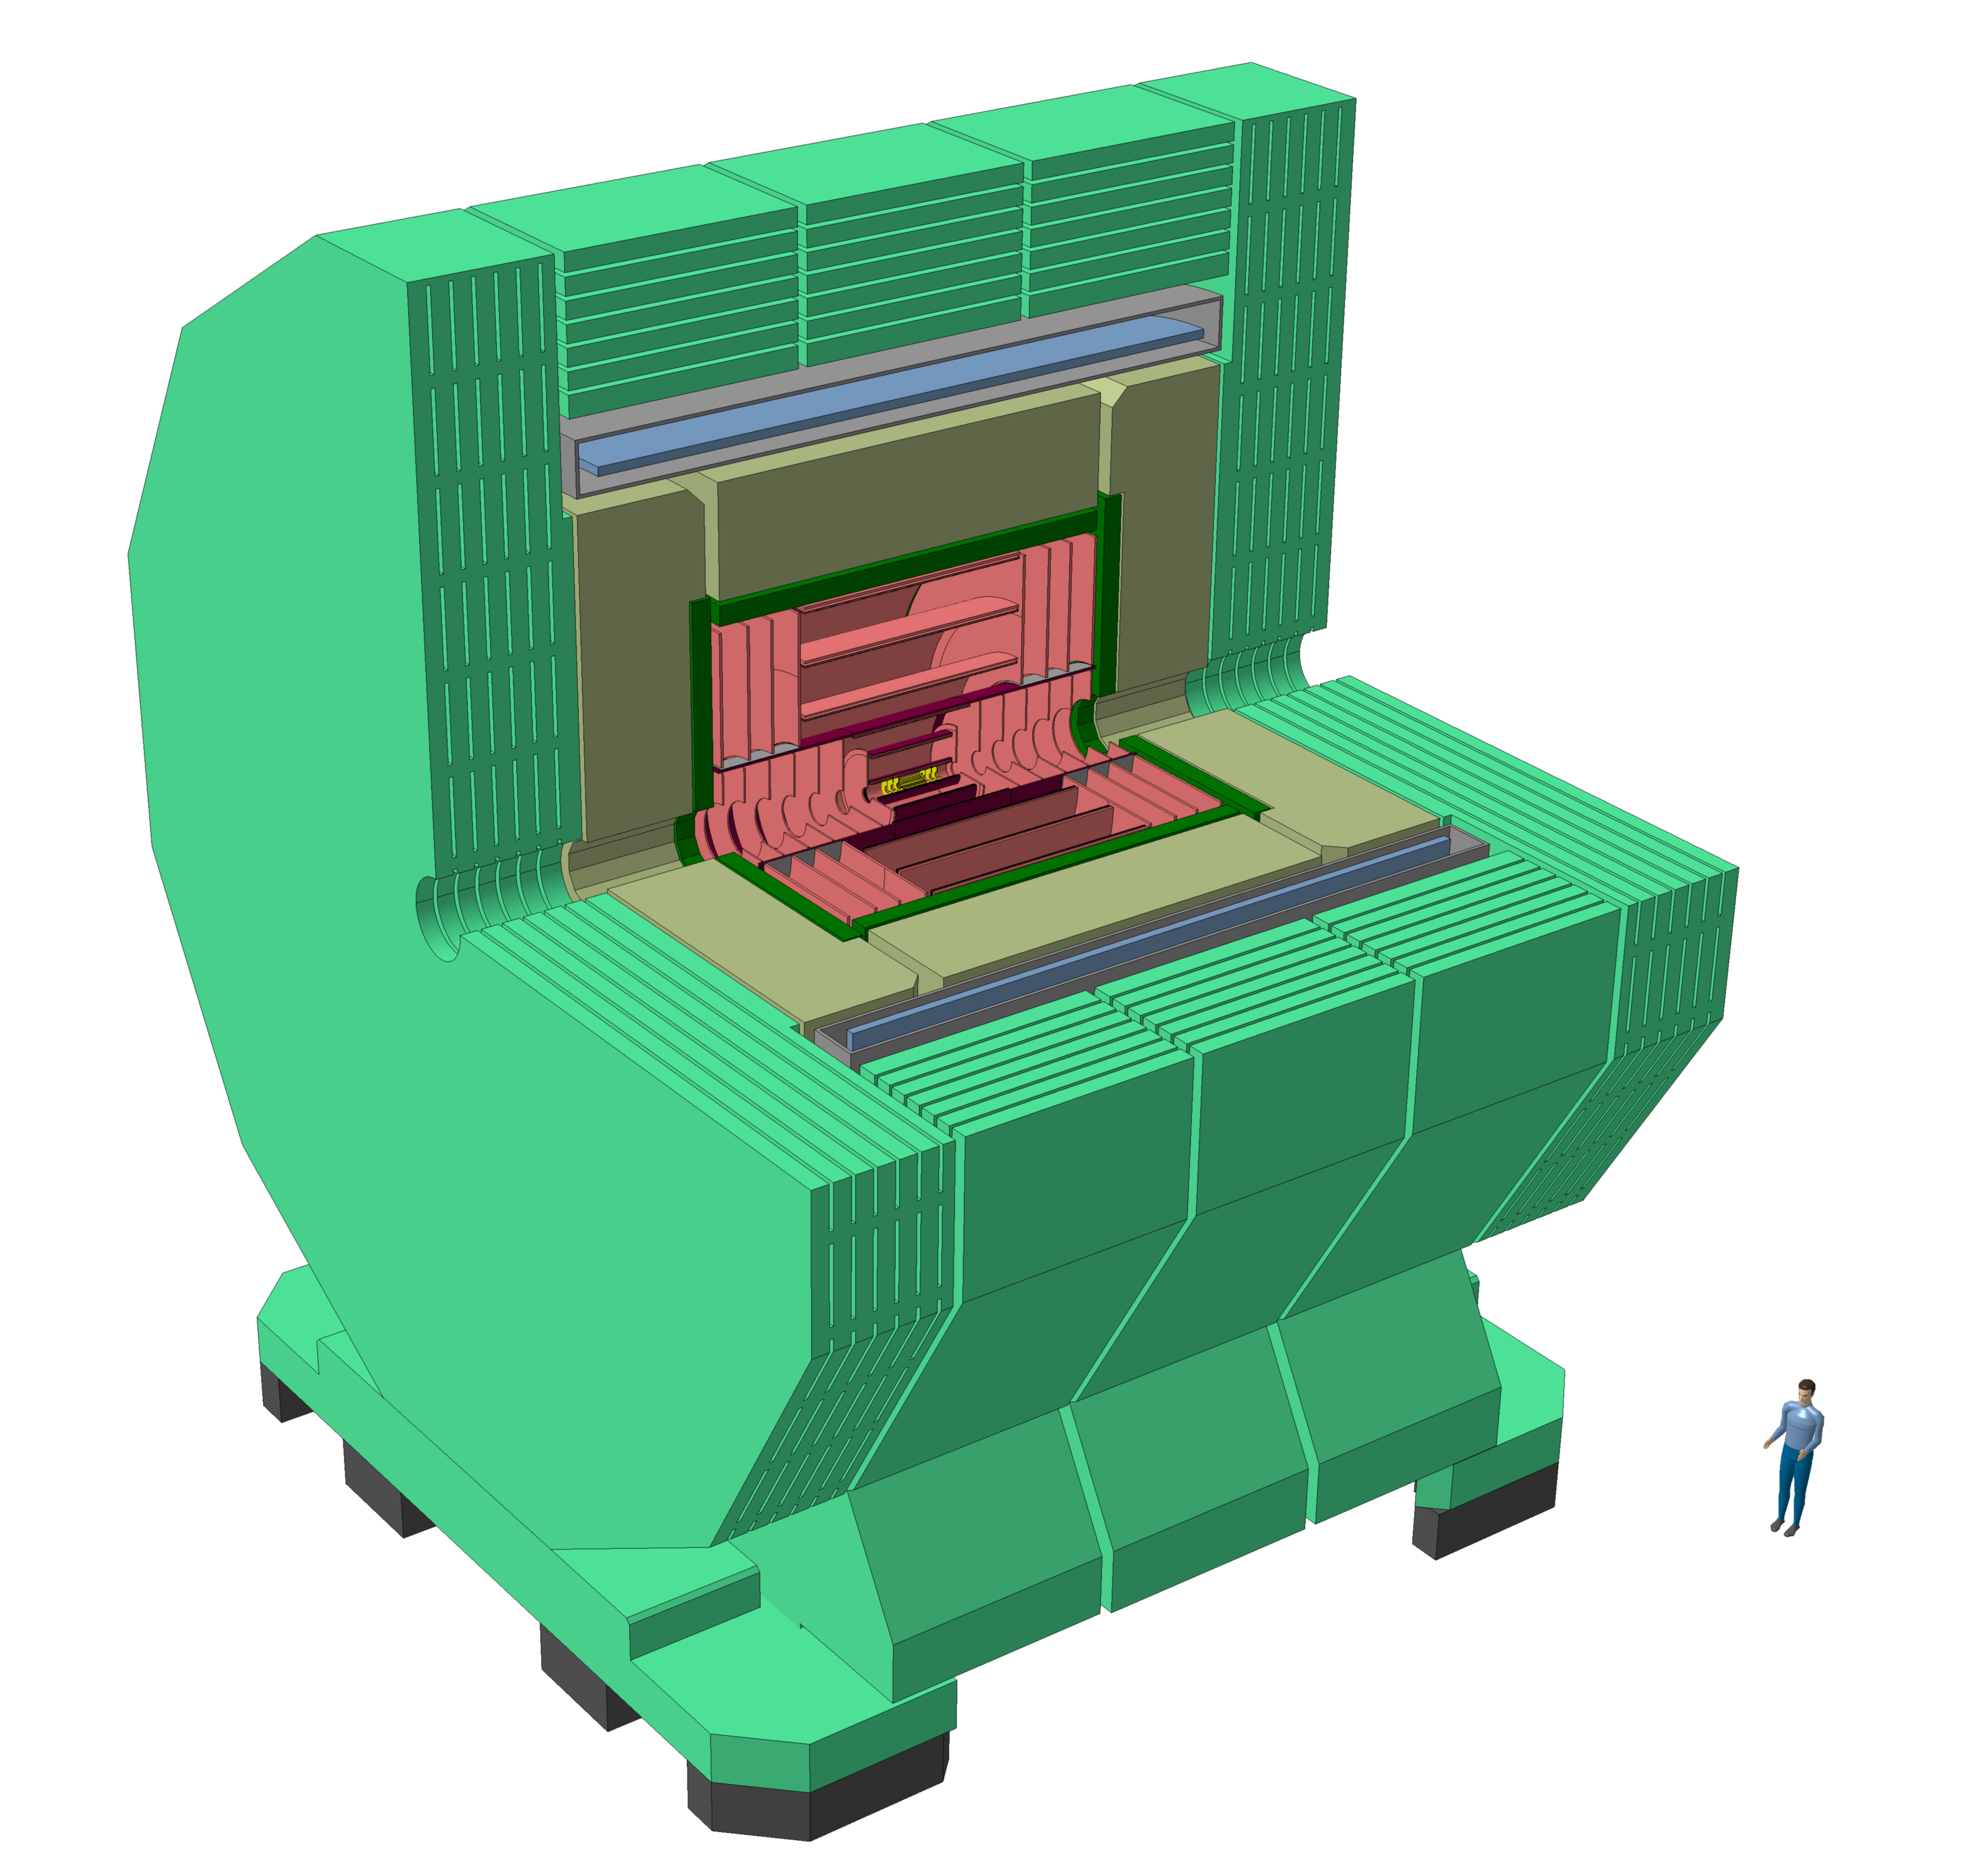
\includegraphics[width=0.82\textwidth]{Figs/commontools/CLD_iso_View.pdf}
  \caption{CLD detector concept view, illustrating a silicon-tracker and particle-flow oriented detector layout. Source: Ref.~\cite{ECFAFactories2025}.}
  \label{fig:cld-view}
\end{figure}
The key lesson is that a projection is meaningful only after the measured observable, the assumptions entering its extraction, and the dominant uncertainty sources have been identified.

Figure~\ref{fig:allegro-view} is used here as a visual anchor for the surrounding discussion. The important point is not only the numerical projection shown in the figure, but also the way in which the relevant FCC observable is connected to a physical parameter of the Standard Model or to a possible deviation from it.
\begin{figure}[H]
  \centering
  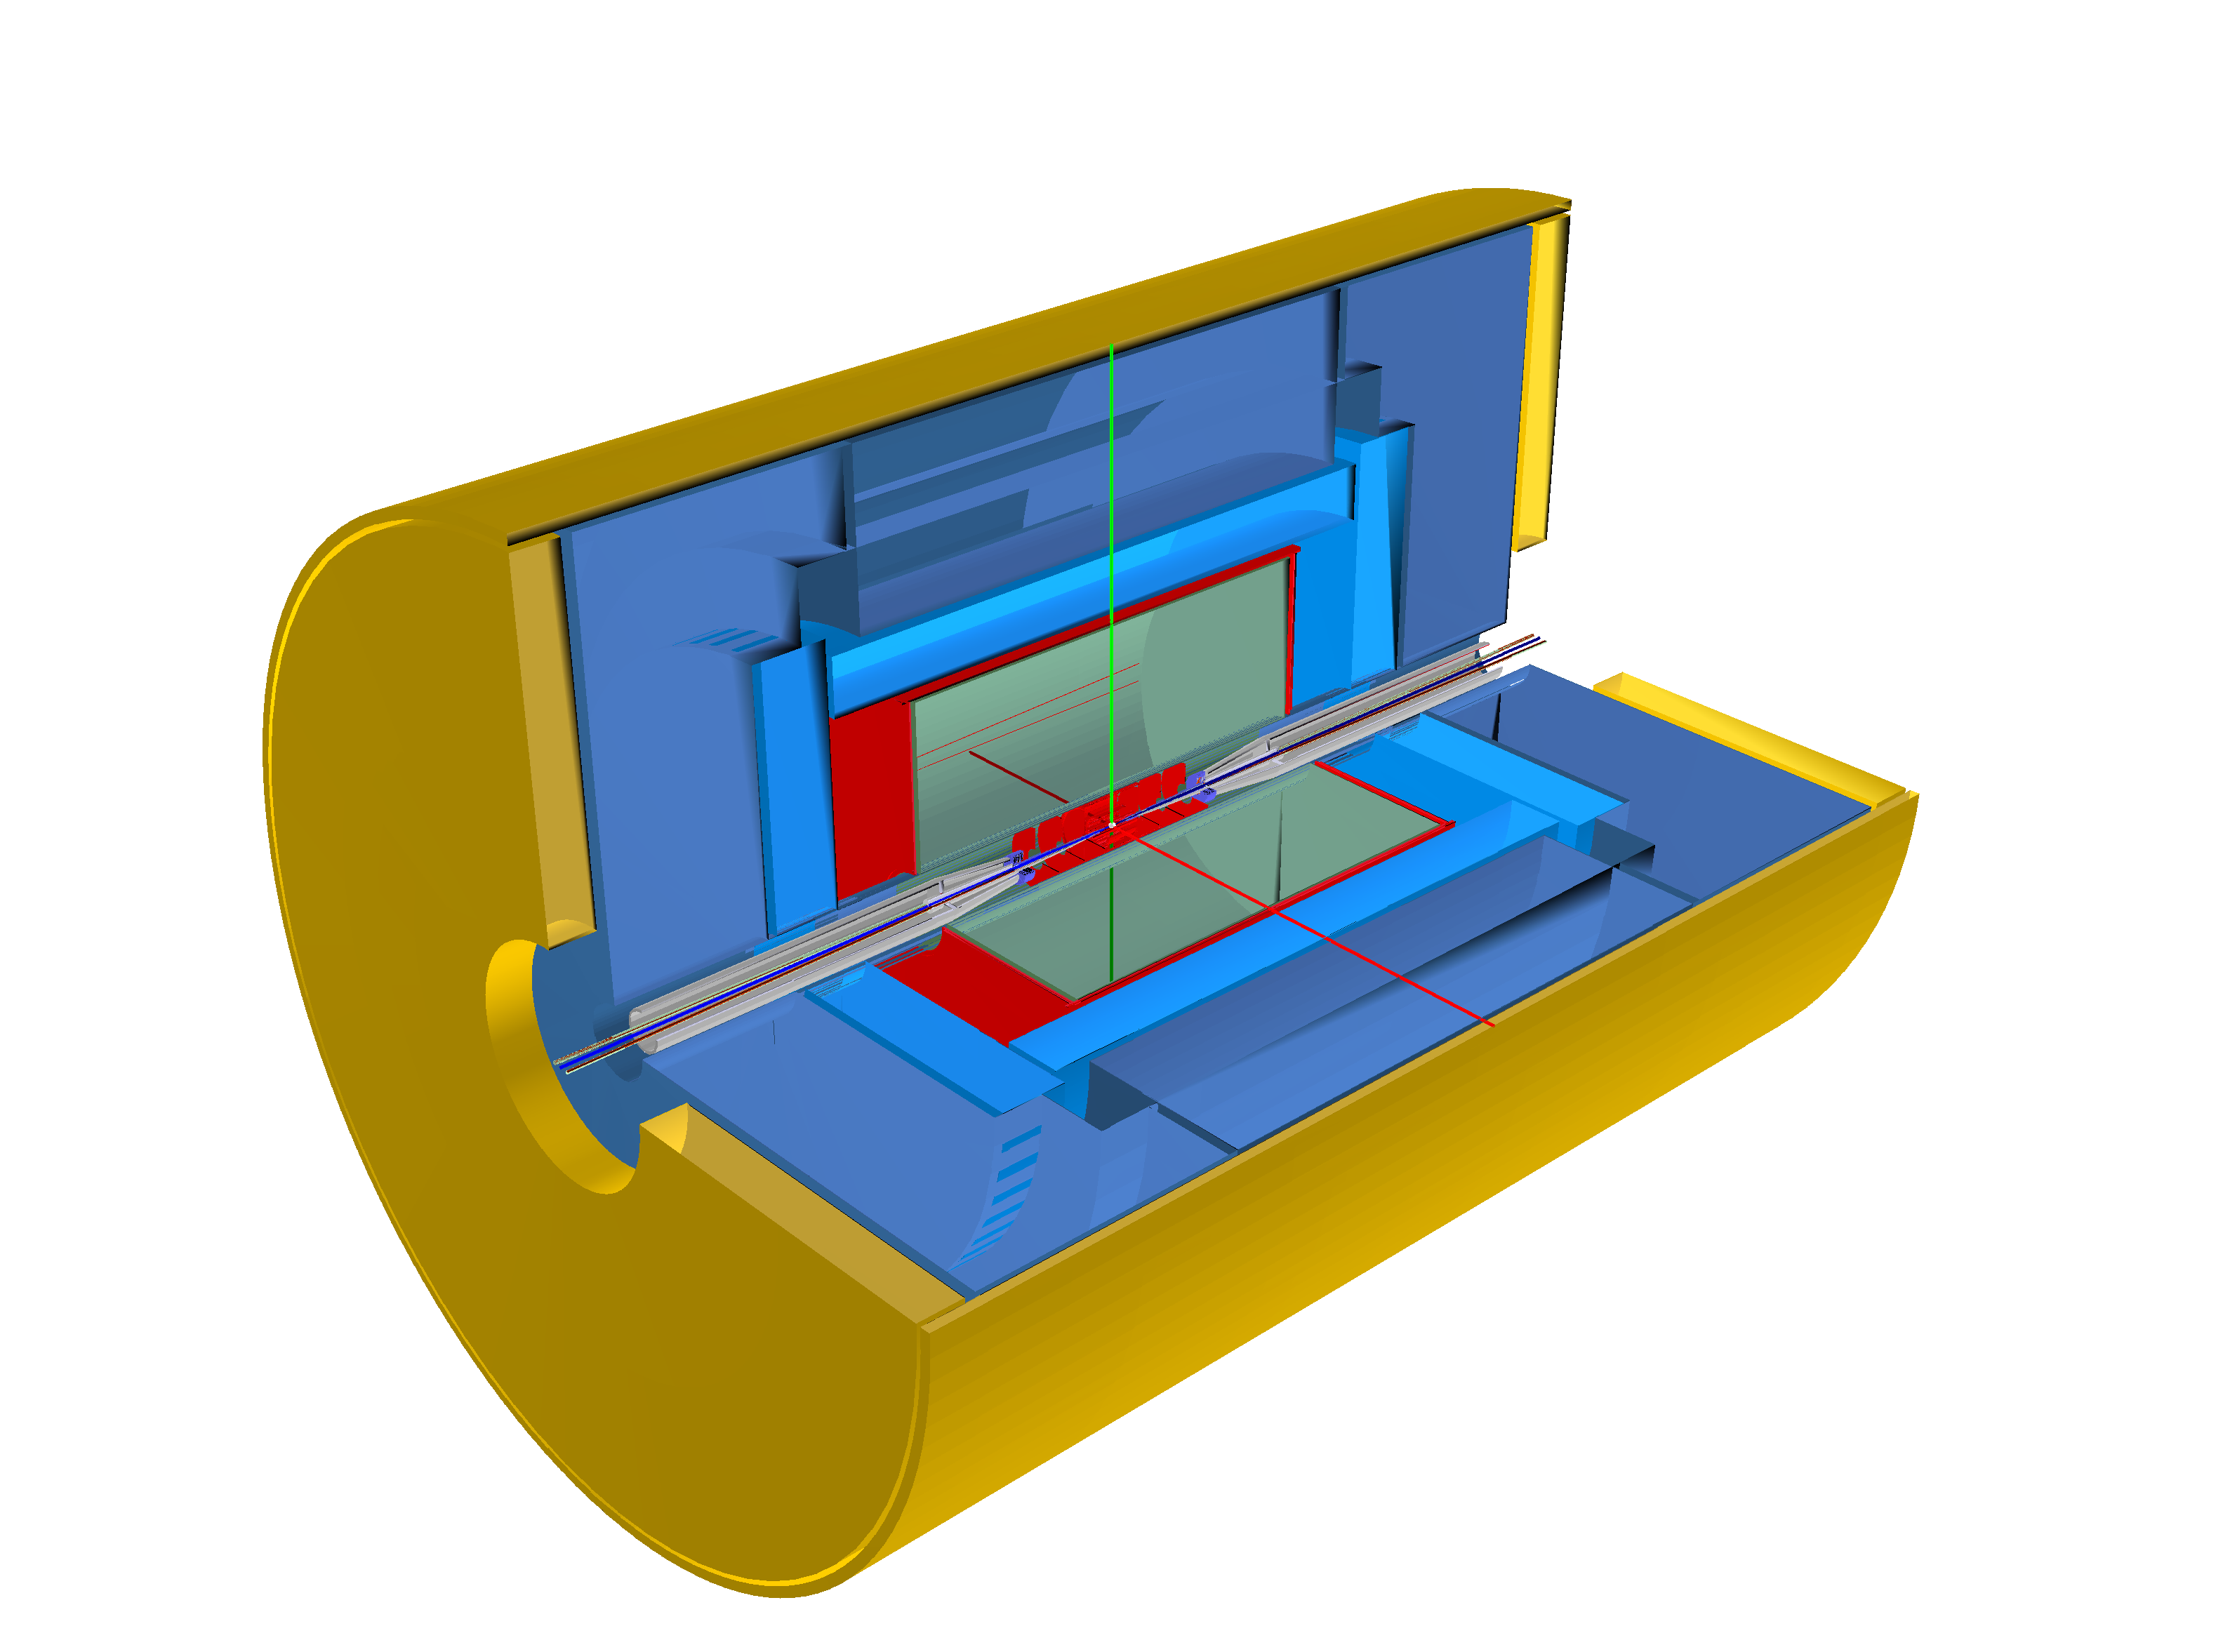
\includegraphics[width=0.82\textwidth]{Figs/commontools/allegro-compressed.pdf}
  \caption{ALLEGRO detector concept, illustrating an alternative detector approach for FCC-ee. Source: Ref.~\cite{ECFAFactories2025}.}
  \label{fig:allegro-view}
\end{figure}
The key lesson is that a projection is meaningful only after the measured observable, the assumptions entering its extraction, and the dominant uncertainty sources have been identified.

Figure~\ref{fig:momentum-resolution} is used here as a visual anchor for the surrounding discussion. The important point is not only the numerical projection shown in the figure, but also the way in which the relevant FCC observable is connected to a physical parameter of the Standard Model or to a possible deviation from it.
\begin{figure}[H]
  \centering
  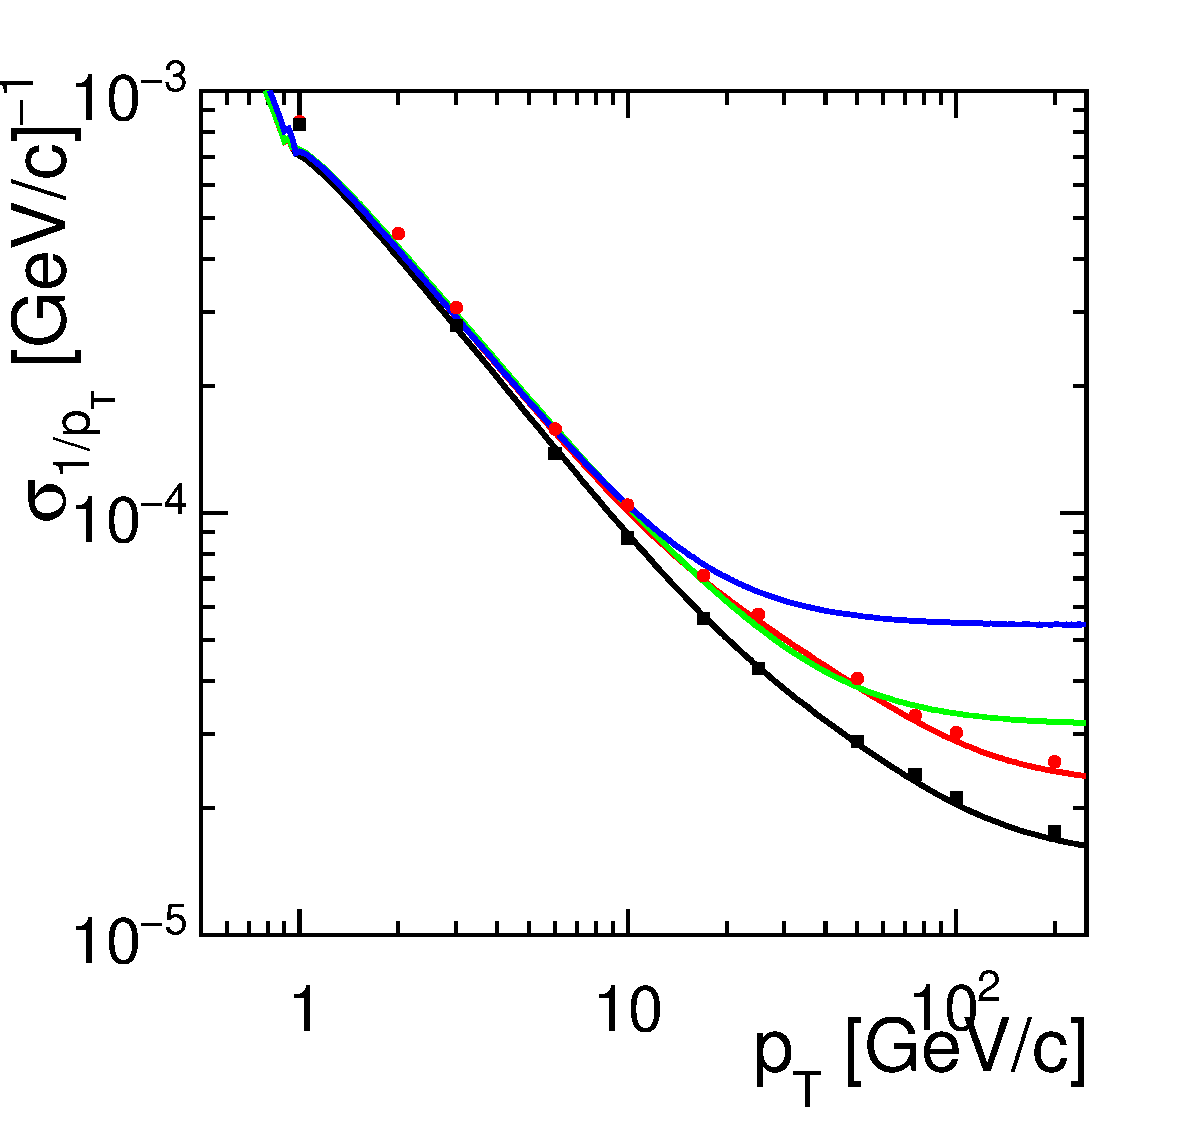
\includegraphics[width=0.75\textwidth]{Figs/commontools/dp_vs_p.pdf}
  \caption{Momentum-resolution performance as a detector requirement for precision measurements. Source: Ref.~\cite{ECFAFactories2025}.}
  \label{fig:momentum-resolution}
\end{figure}
The key lesson is that a projection is meaningful only after the measured observable, the assumptions entering its extraction, and the dominant uncertainty sources have been identified.

\begin{definition}{Jet flavour tagging}{flavour-tagging}
Jet flavour tagging is the classification of jets as likely originating from \(b\), \(c\), light quarks or gluons. At FCC-ee it is essential for Higgs couplings, electroweak heavy-flavour observables, flavour physics and many BSM searches.
\end{definition}

\subsection{Tracking, vertexing and particle identification}
The impact-parameter resolution can be parametrised schematically as
\begin{equation}
  \sigma_{d_0}=a\oplus \frac{b}{p\sin^{3/2}\theta},
\end{equation}
where \(a\) is a detector-intrinsic term and \(b\) reflects multiple scattering. Excellent vertexing is needed for heavy-flavour tagging and displaced vertices. Particle identification improves separation of kaons, pions, protons, electrons and muons, and is especially important for flavour and tau studies.

\subsection{Calorimetry and particle flow}
Higgs and electroweak measurements rely on reconstructing jets, photons, missing momentum and neutral hadrons. Particle-flow reconstruction combines information from tracking and calorimetry to avoid double counting and improve jet energy resolution. Dual-readout calorimetry, high-granularity calorimetry and noble-liquid options appear in different FCC detector concepts; the lecture-note point is that detector choices are linked to physics channels.

Figure~\ref{fig:edm4hep} is used here as a visual anchor for the surrounding discussion. The important point is not only the numerical projection shown in the figure, but also the way in which the relevant FCC observable is connected to a physical parameter of the Standard Model or to a possible deviation from it.
\begin{figure}[H]
  \centering
  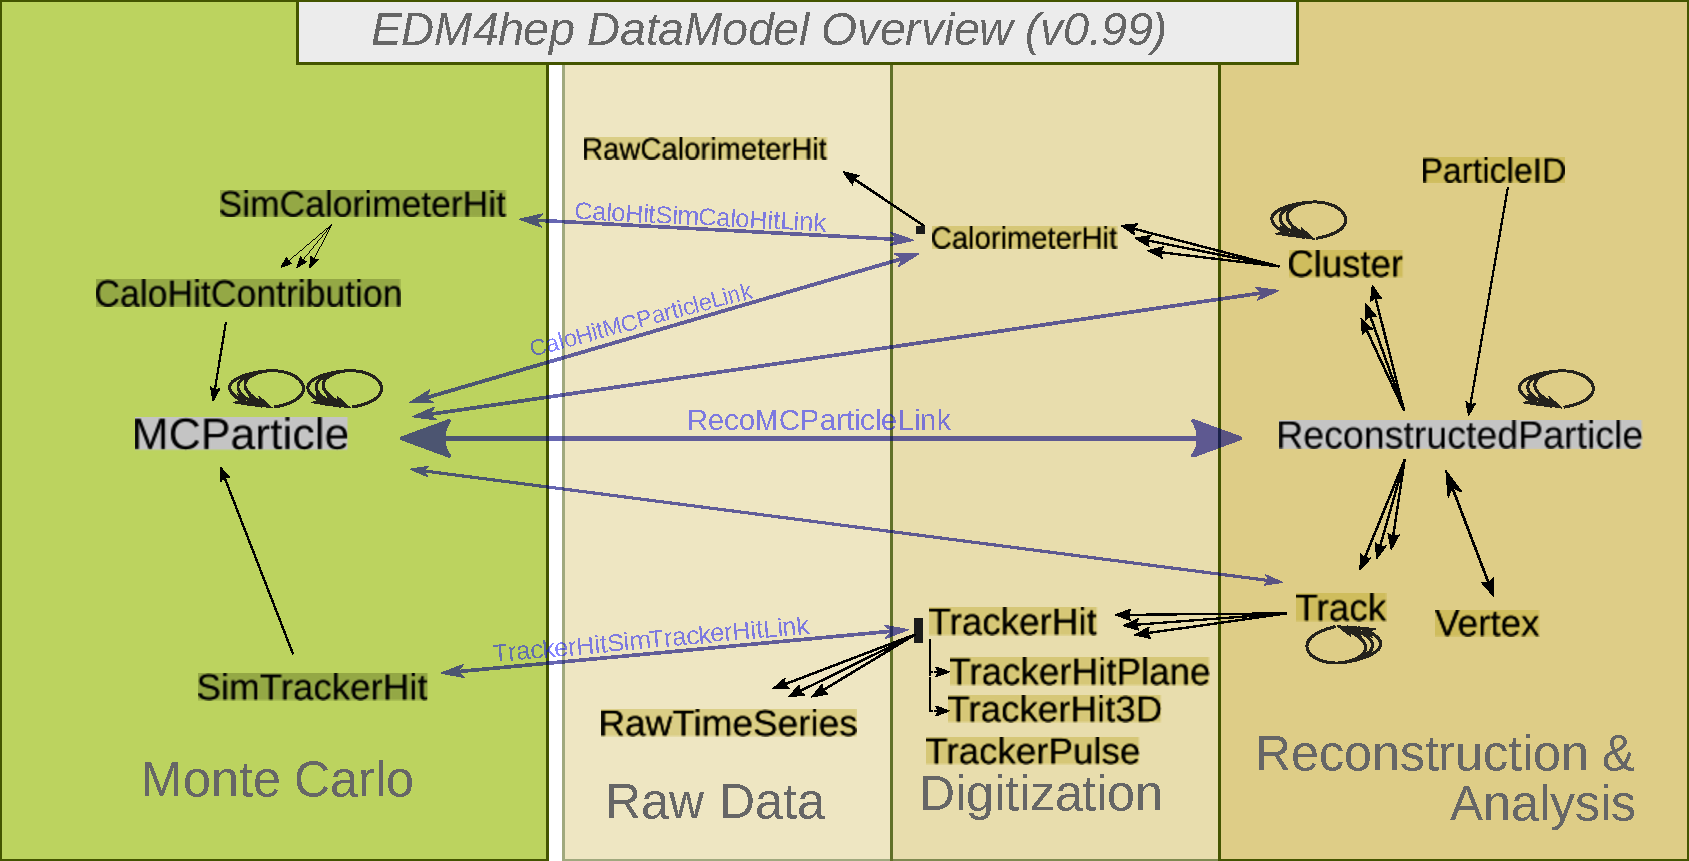
\includegraphics[width=0.82\textwidth]{Figs/commontools/edm4hep_diagram_v99.pdf}
  \caption{EDM4hep event-data model diagram used in the common software ecosystem. Source: Ref.~\cite{Key4hep2022}.}
  \label{fig:edm4hep}
\end{figure}
The key lesson is that a projection is meaningful only after the measured observable, the assumptions entering its extraction, and the dominant uncertainty sources have been identified.

Figure~\ref{fig:key4hep} is used here as a visual anchor for the surrounding discussion. The important point is not only the numerical projection shown in the figure, but also the way in which the relevant FCC observable is connected to a physical parameter of the Standard Model or to a possible deviation from it.
\begin{figure}[H]
  \centering
  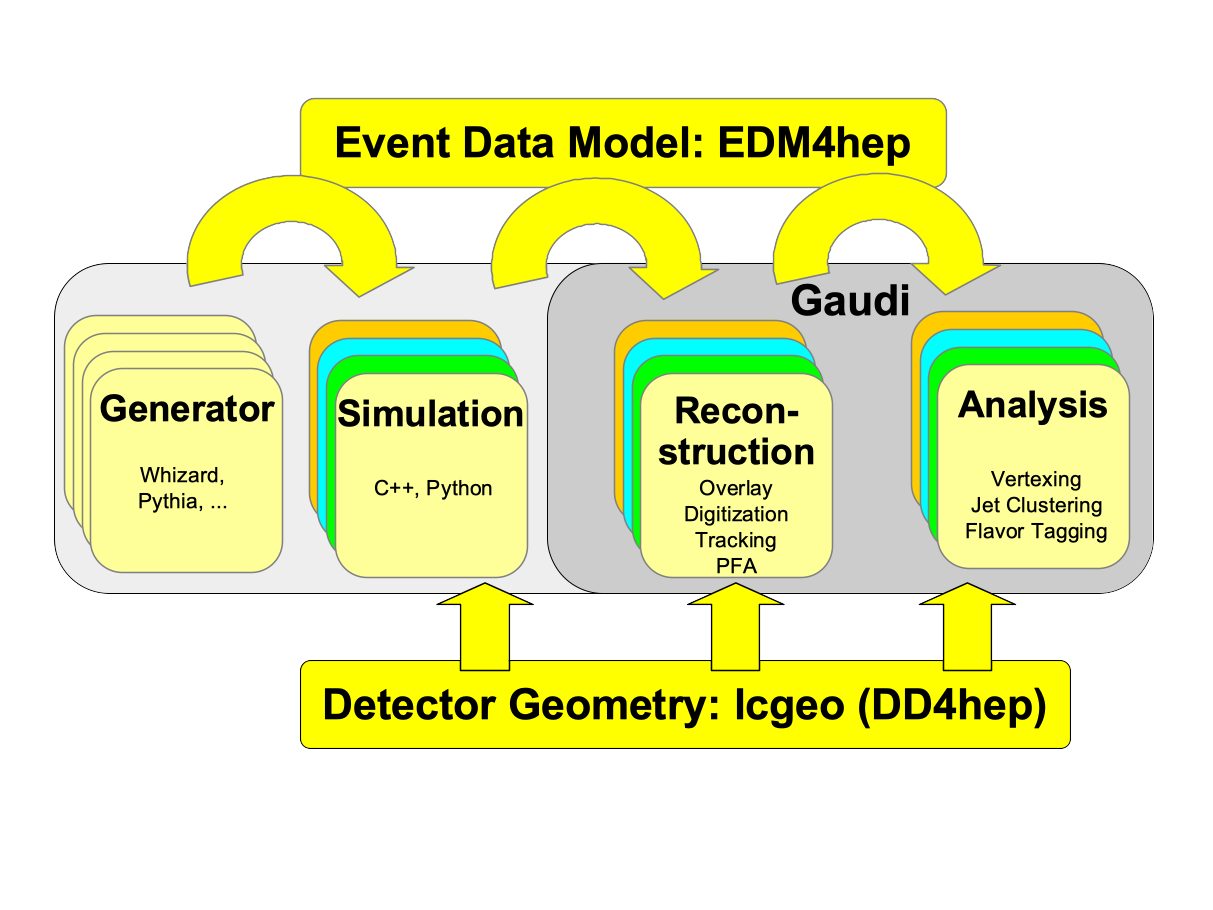
\includegraphics[width=0.86\textwidth]{Figs/commontools/key4hep_chain_gaudi.png}
  \caption{Key4hep/Gaudi-based software chain for simulation, reconstruction and analysis. Source: Ref.~\cite{Key4hep2022}.}
  \label{fig:key4hep}
\end{figure}
The key lesson is that a projection is meaningful only after the measured observable, the assumptions entering its extraction, and the dominant uncertainty sources have been identified.

\subsection{Software: Key4hep and EDM4hep}
The FCC software ecosystem aims to provide common tools for detector description, simulation, reconstruction and analysis. EDM4hep defines a common event-data model, while Key4hep provides the software environment in which multiple future-collider detector studies can share infrastructure. This is important for reproducibility and for comparing detector concepts under similar assumptions.

\begin{examplebox}{Detector requirement from \(H	o c\bar c\)}{hcc-detector-example}
The \(H\to c\bar c\) coupling requires separation of charm jets from bottom and light jets. A high charm-tagging efficiency with controlled b-jet and light-jet mistag rates depends on vertex detector resolution, tracking efficiency, material budget, and multivariate flavour-tagging algorithms. Thus a Higgs coupling number is ultimately tied to detector technology.
\end{examplebox}

\begin{guidedchecksbox}
\begin{enumerate}[leftmargin=1.6em]
\item Why does the recoil method require excellent lepton momentum resolution?
\item Explain why PID is valuable for flavour physics but less central for inclusive \(ZH\) counting.
\item List three ways detector systematics can enter a global Higgs coupling fit.
\end{enumerate}
\end{guidedchecksbox}

\subsection{Exercises}
\begin{enumerate}[leftmargin=1.6em]
\item Explain how an uncertainty in b-tagging efficiency propagates into \(H\to b\bar b\) coupling measurements.
\item Compare full simulation and fast simulation in terms of speed, realism and systematic control.
\item Describe the role of a common event-data model in a multi-detector future-collider programme.
\end{enumerate}


\newpage
\section{FCC-hh and the integrated programme}
\begin{guidelinebox}
FCC-hh extends the FCC programme to the energy frontier, building on the FCC-hh CDR and broader 100 TeV collider studies~\cite{FCCCDRVol3,ArkaniHamed100TeV2016,ManganoFCChh2017}. Its role is not only to search for new heavy particles, but also to complete the Higgs programme, test high-energy tails and provide direct access to physics that may first appear indirectly at FCC-ee.
\end{guidelinebox}

\subsection{Direct search reach}
At FCC-hh, representative processes include
\begin{equation}
  pp\to Z',\ W',\ \tilde q\tilde q,\ \tilde g\tilde g,\ X_{\rm BSM},
\end{equation}
with subsequent decays into leptons, jets, missing energy, Higgs bosons or electroweak bosons. The exact reach depends on parton luminosities, backgrounds, detector performance and integrated luminosity. The gain relative to the LHC comes from both energy and luminosity.

Figure~\ref{fig:fcchh-reach} is used here as a visual anchor for the surrounding discussion. The important point is not only the numerical projection shown in the figure, but also the way in which the relevant FCC observable is connected to a physical parameter of the Standard Model or to a possible deviation from it.
\begin{figure}[H]
  \centering
  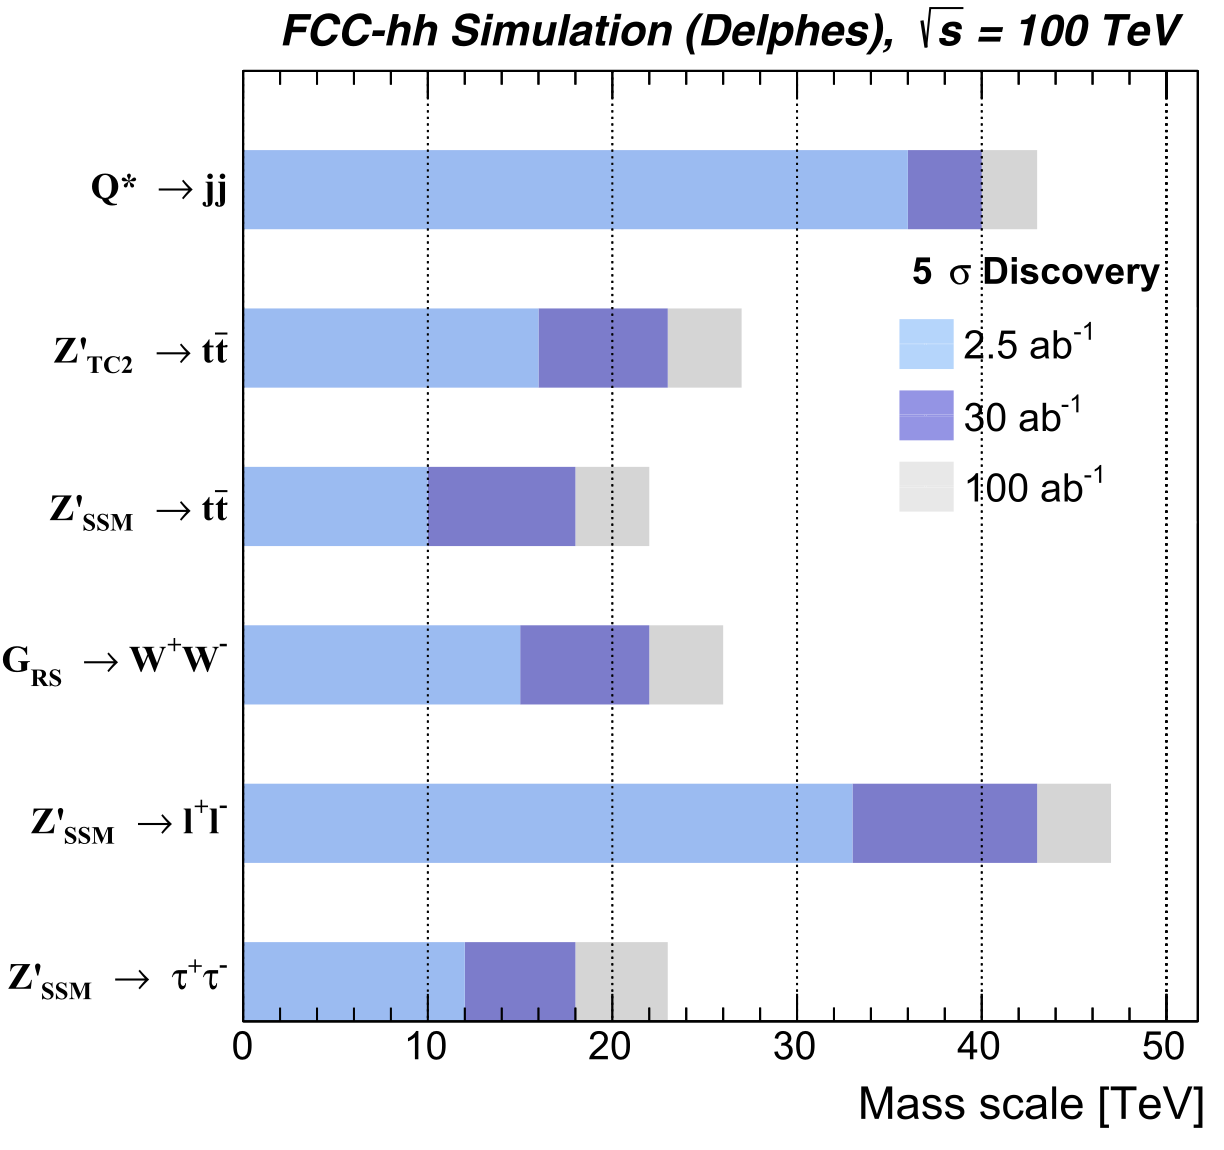
\includegraphics[width=0.86\textwidth]{Figs/FCCHHschannelreach.png}
  \caption{FCC-hh s-channel resonance discovery reach as a function of resonance mass and luminosity. Source: Ref.~\cite{FCCFSRVol1}.}
  \label{fig:fcchh-reach}
\end{figure}
The key lesson is that a projection is meaningful only after the measured observable, the assumptions entering its extraction, and the dominant uncertainty sources have been identified.

Figure~\ref{fig:pair-comp} is used here as a visual anchor for the surrounding discussion. The important point is not only the numerical projection shown in the figure, but also the way in which the relevant FCC observable is connected to a physical parameter of the Standard Model or to a possible deviation from it.
\begin{figure}[H]
  \centering
  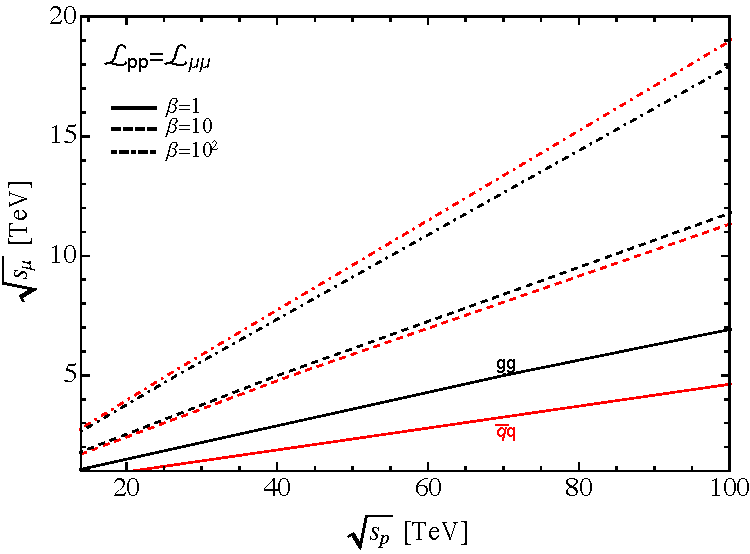
\includegraphics[width=0.86\textwidth]{Figs/PairComp.pdf}
  \caption{Pair-production reach comparison for future collider options. Source: Ref.~\cite{FCCFSRVol1}.}
  \label{fig:pair-comp}
\end{figure}
The key lesson is that a projection is meaningful only after the measured observable, the assumptions entering its extraction, and the dominant uncertainty sources have been identified.

Figure~\ref{fig:resonance-comp} is used here as a visual anchor for the surrounding discussion. The important point is not only the numerical projection shown in the figure, but also the way in which the relevant FCC observable is connected to a physical parameter of the Standard Model or to a possible deviation from it.
\begin{figure}[H]
  \centering
  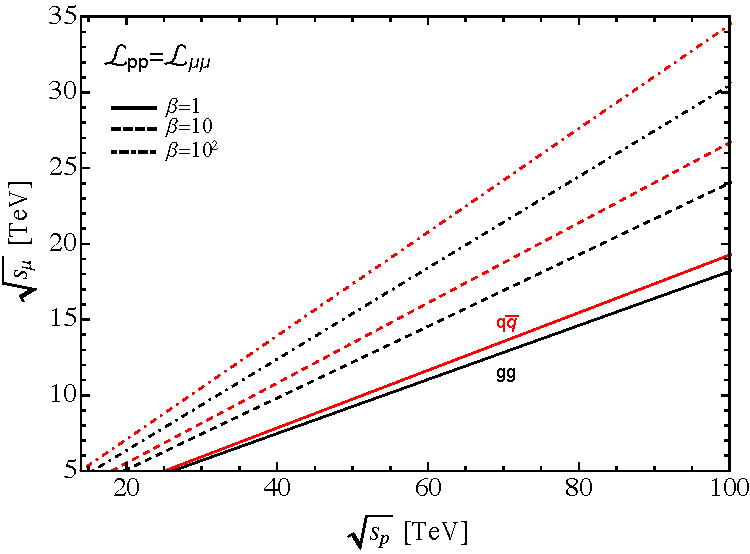
\includegraphics[width=0.86\textwidth]{Figs/ResonanceComp.pdf}
  \caption{Resonance-search reach comparison for future collider options. Source: Ref.~\cite{FCCFSRVol1}.}
  \label{fig:resonance-comp}
\end{figure}
The key lesson is that a projection is meaningful only after the measured observable, the assumptions entering its extraction, and the dominant uncertainty sources have been identified.

\subsection{Higgs self-coupling at FCC-hh}
Double-Higgs production is the direct route to the trilinear coupling:
\begin{equation}
  pp\to HH+X .
\end{equation}
A useful schematic dependence is
\begin{equation}
  \sigma(pp\to HH)=\sigma_{\SM}\left[1+a(\kappa_\lambda-1)+b(\kappa_\lambda-1)^2\right],
\end{equation}
where \(a\) and \(b\) depend on collider energy, fiducial phase space and analysis selection. FCC-hh can substantially improve the precision on \(\kappa_\lambda\), while FCC-ee provides complementary loop-level constraints in single-Higgs processes.

Figure~\ref{fig:hself-precision} is used here as a visual anchor for the surrounding discussion. The important point is not only the numerical projection shown in the figure, but also the way in which the relevant FCC observable is connected to a physical parameter of the Standard Model or to a possible deviation from it.
\begin{figure}[H]
  \centering
  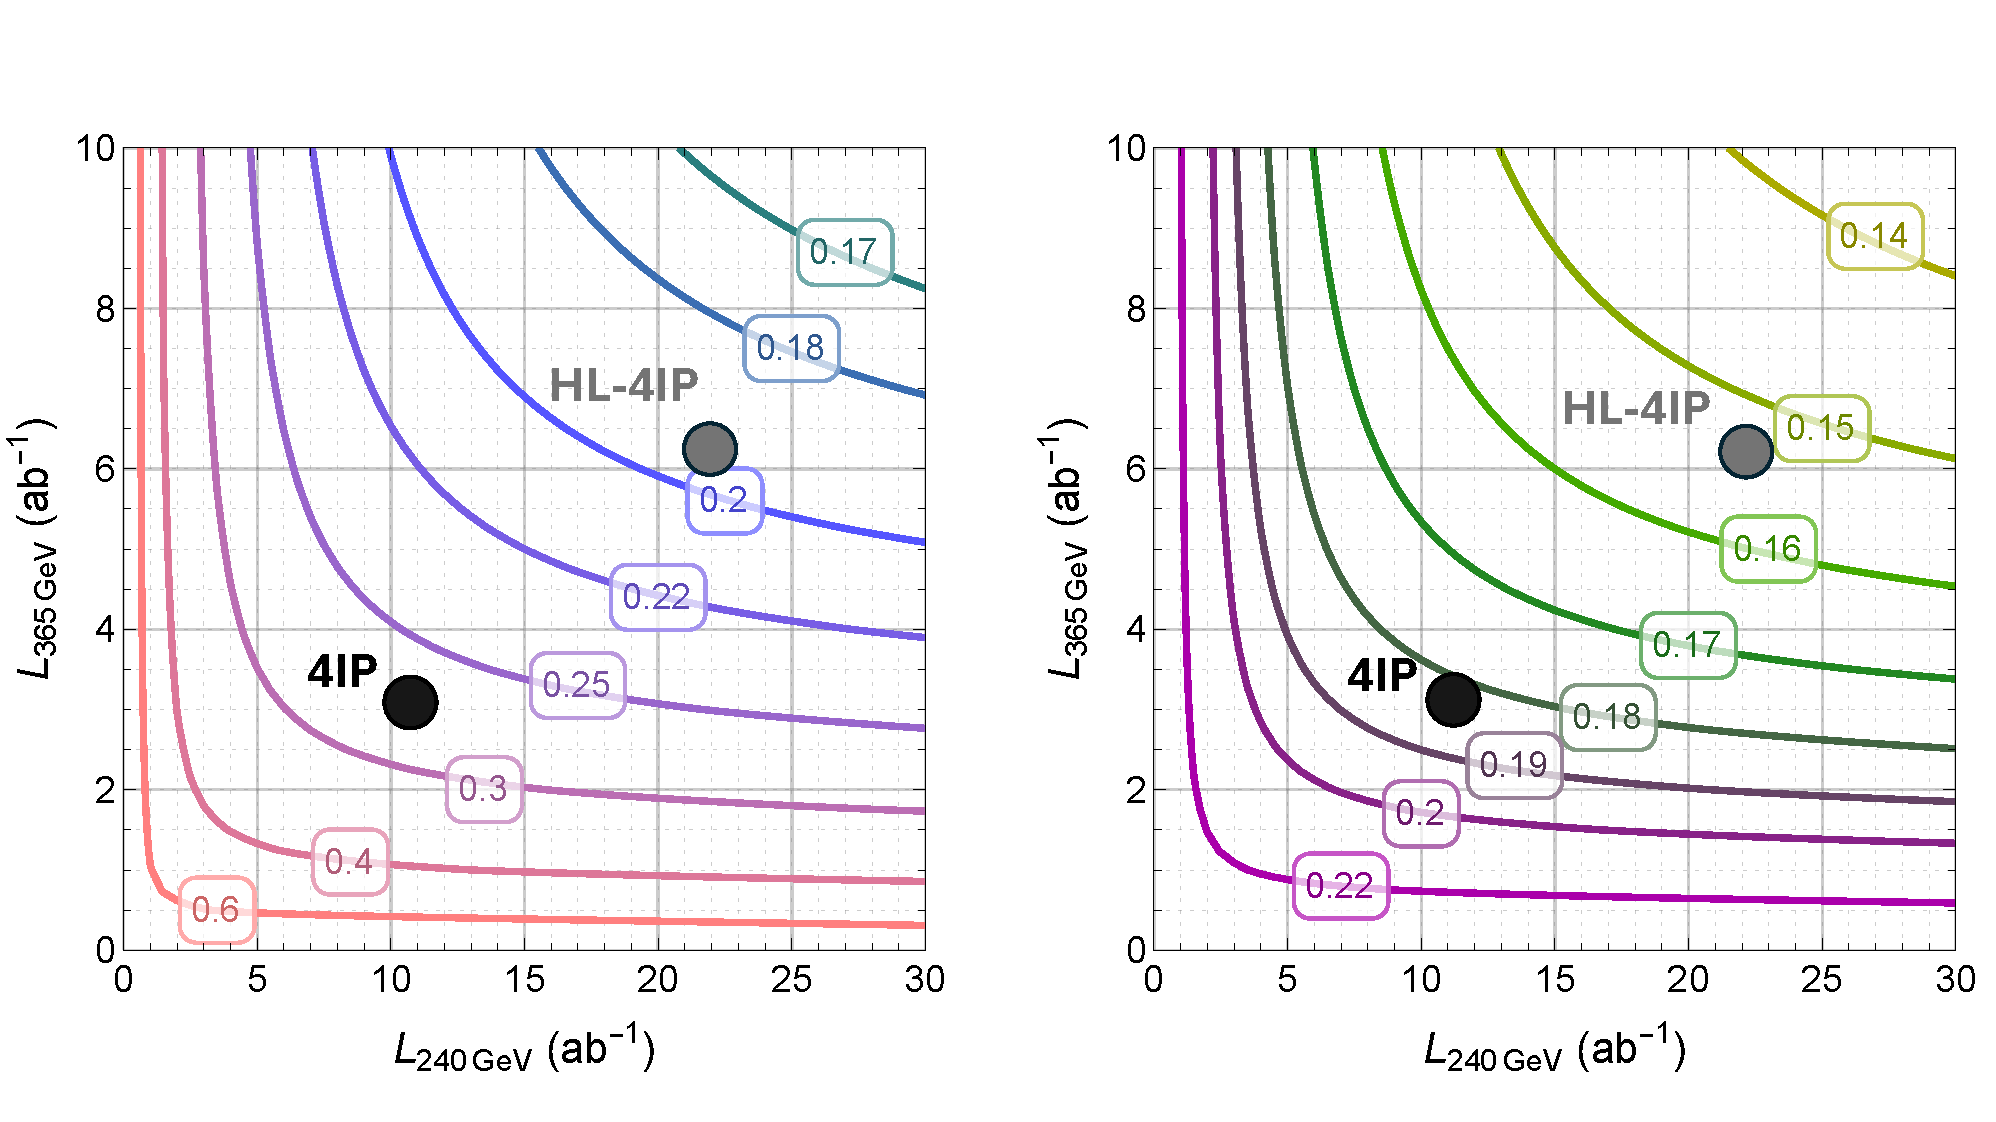
\includegraphics[width=0.86\textwidth]{Figs/Hselfcoupling-precision-1b.pdf}
  \caption{Projected precision on the Higgs self-coupling in future collider programmes. Source: Ref.~\cite{FCCFSRVol1}.}
  \label{fig:hself-precision}
\end{figure}
The key lesson is that a projection is meaningful only after the measured observable, the assumptions entering its extraction, and the dominant uncertainty sources have been identified.

Figure~\ref{fig:neutrino-spectra} is used here as a visual anchor for the surrounding discussion. The important point is not only the numerical projection shown in the figure, but also the way in which the relevant FCC observable is connected to a physical parameter of the Standard Model or to a possible deviation from it.
\begin{figure}[H]
  \centering
  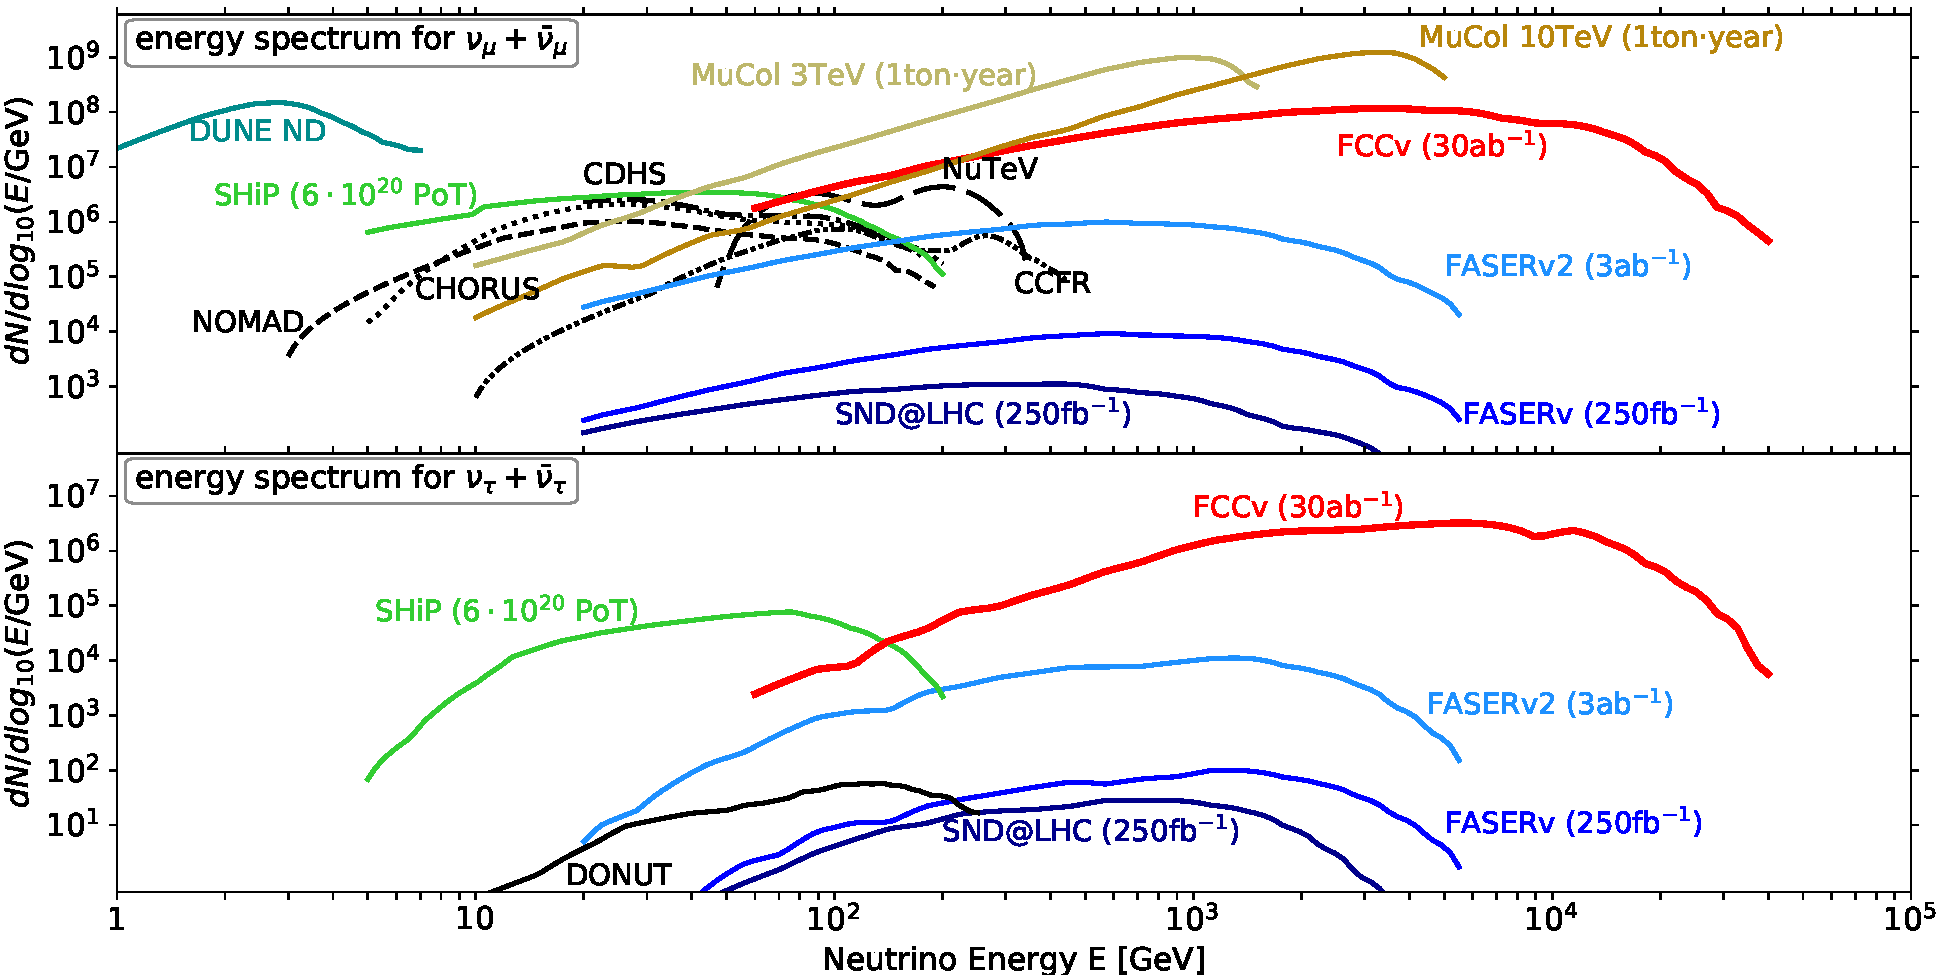
\includegraphics[width=0.80\textwidth]{Figs/NeutrinoSpectra.pdf}
  \caption{Illustrative neutrino spectra for forward physics opportunities at FCC-hh. Source: Ref.~\cite{FCCFSRVol1}.}
  \label{fig:neutrino-spectra}
\end{figure}
The key lesson is that a projection is meaningful only after the measured observable, the assumptions entering its extraction, and the dominant uncertainty sources have been identified.

\subsection{High-energy precision and SMEFT tails}
High-mass Drell--Yan, vector-boson scattering, associated Higgs production and boosted final states probe energy-growing SMEFT effects,
\begin{equation}
  \frac{\delta\sigma}{\sigma}\sim C_i\frac{\hat s}{\Lambda^2} .
\end{equation}
This is complementary to FCC-ee, where the clean environment and Z-pole precision dominate many electroweak constraints. The best physics interpretation combines low-energy precision with high-energy tails and direct searches.

\begin{remarkbox}{Integrated does not mean redundant}{integrated-not-redundant}
FCC-ee and FCC-hh probe different directions in theory space. FCC-ee is often superior for weakly coupled electroweak and flavour effects, while FCC-hh is essential for direct production at tens of TeV and for rare high-energy processes. The integrated programme is powerful precisely because the two stages are not identical.
\end{remarkbox}

\begin{guidedchecksbox}
\begin{enumerate}[leftmargin=1.6em]
\item Explain why a heavy resonance may be found directly at FCC-hh but only indirectly at FCC-ee.
\item Give an example where FCC-ee precision would help interpret an FCC-hh discovery.
\item Explain why high-energy tails can enhance SMEFT sensitivity.
\end{enumerate}
\end{guidedchecksbox}

\subsection{Exercises}
\begin{enumerate}[leftmargin=1.6em]
\item Sketch the interference between triangle and box diagrams in \(gg\to HH\) and explain why the cross section is not a linear function of \(\kappa_\lambda\).
\item Compare the sensitivity of FCC-ee and FCC-hh to a weakly coupled dark sector and to a strongly produced coloured resonance.
\item Explain why parton luminosities matter for FCC-hh mass reach.
\end{enumerate}


\newpage
\section{Summary and outlook}
\begin{guidelinebox}
This final chapter collects the main conceptual messages. The FCC precision programme is not a list of independent measurements; it is a correlated set of Standard Model closure tests and BSM probes whose power depends on experiment, theory, detector design and global interpretation.
\end{guidelinebox}

\subsection{Core messages}
\begin{enumerate}[leftmargin=1.6em]
\item FCC-ee provides extremely clean and high-statistics samples of Z bosons, W pairs, Higgs bosons and top quarks.
\item The Higgs recoil method is the key to absolute Higgs coupling and width determinations.
\item The Tera-Z and WW-threshold programmes sharpen electroweak closure tests and improve inputs to Higgs and SMEFT fits.
\item The top-threshold scan can measure a theoretically well-defined top mass, but the final interpretation requires high-order QCD and electroweak calculations.
\item SMEFT and effective-coupling interpretations require global fits because Higgs, electroweak, top and diboson observables are correlated.
\item Flavour, tau and BSM searches are integral to the programme, not optional additions.
\item FCC-hh completes the integrated programme through direct high-mass searches, high-energy precision and direct Higgs self-coupling sensitivity.
\end{enumerate}

Figure~\ref{fig:ped-groups} is used here as a visual anchor for the surrounding discussion. The important point is not only the numerical projection shown in the figure, but also the way in which the relevant FCC observable is connected to a physical parameter of the Standard Model or to a possible deviation from it.
\begin{figure}[H]
  \centering
  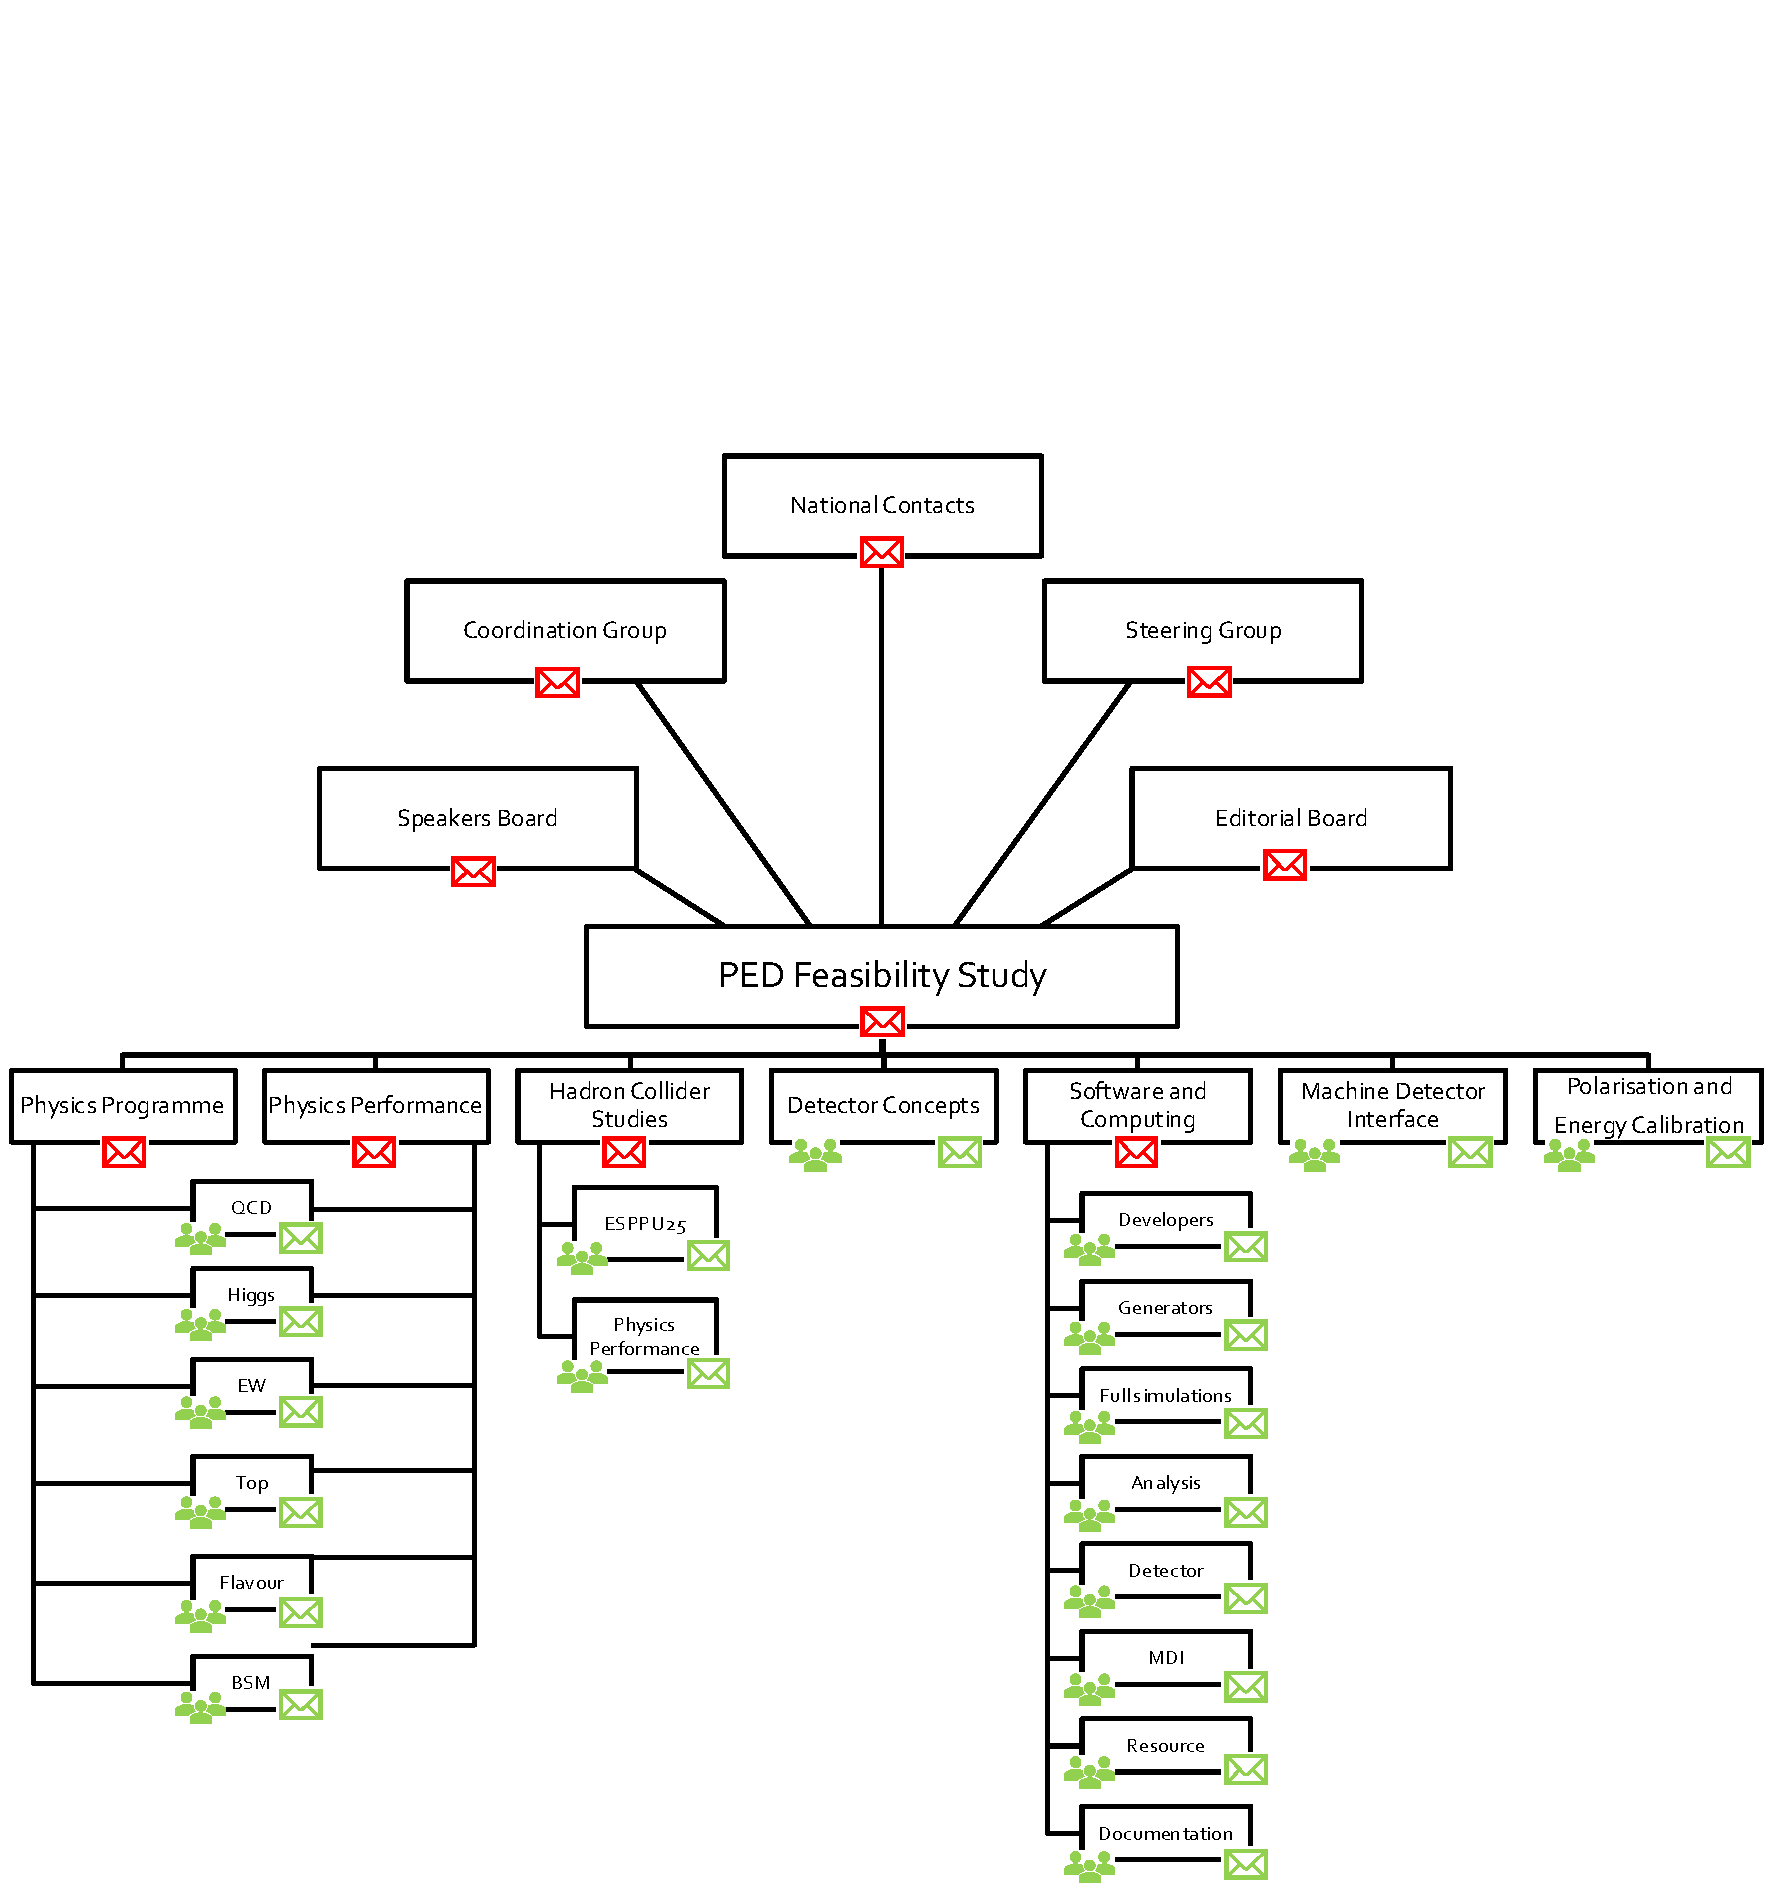
\includegraphics[width=0.80\textwidth]{Figs/PED_e-groups.pdf}
  \caption{Physics, experiments and detectors organisation schematic. Source: Ref.~\cite{FCCFSRVol1}.}
  \label{fig:ped-groups}
\end{figure}
The key lesson is that a projection is meaningful only after the measured observable, the assumptions entering its extraction, and the dominant uncertainty sources have been identified.

\subsection{Summary table of physics pillars}
\begin{table}[H]
\centering
\scriptsize
\caption{Conceptual summary of FCC precision-physics pillars.}
\label{tab:summary-pillars}
\begin{tabularx}{\textwidth}{@{}p{2.2cm}p{4.0cm}X@{}}
\toprule
Pillar & Representative observables & Main interpretation role\\
\midrule
Higgs & \(\sigma_{ZH}\), \(\BR(H\to X)\), \(\Gamma_H\), \(\kappa_i\) & Absolute couplings, invisible/exotic decays, Higgs potential.\\
Electroweak & \(\mZ,\Gamma_Z,\sigma^0_{\rm had},\sintw,\mW\) & Closure tests, weak mixing, input parameters, SMEFT currents.\\
Top & \(m_t^{\rm PS},\Gamma_t,y_t,t\bar tZ\) couplings & Mass scheme, electroweak/top sector, Higgs-top interplay.\\
Flavour/tau & Rare \(b,c,\tau\) decays, LFV, LFU & Flavour structure, third-generation BSM, rare processes.\\
BSM/LLP & HNLs, ALPs, exotic Z/H decays, displaced vertices & Feebly coupled sectors and hidden particles.\\
FCC-hh & Resonances, pair production, \(HH\), high-energy tails & Energy-frontier completion and direct discovery.\\
\bottomrule
\end{tabularx}
\end{table}

\begin{takehomebox}
The central scientific promise of the FCC is not merely a smaller error bar on one parameter. It is an overconstrained map of the electroweak scale, the Higgs sector, flavour, top physics and possible new interactions.
\end{takehomebox}

\begin{guidedchecksbox}
\begin{enumerate}[leftmargin=1.6em]
\item Identify one measurement in the lecture note that is mainly statistics driven and one that is mainly systematics/theory driven.
\item Explain why the FCC-ee Higgs programme depends on the electroweak programme.
\item Give a possible research project based on one figure or observable discussed in the note.
\end{enumerate}
\end{guidedchecksbox}

\subsection{Open research directions for students}
\begin{itemize}[leftmargin=1.6em]
\item Updating Higgs coupling fits with the latest FCC-ee run scenario and theory uncertainties.
\item Studying flavour-tagging assumptions for \(H\to c\bar c\), \(H\to b\bar b\) and \(H\to gg\).
\item Testing the stability of SMEFT fits under different flavour assumptions.
\item Exploring top-FCNC sensitivity at 365 GeV using realistic reconstruction assumptions.
\item Comparing exotic Higgs decay searches in prompt and displaced regimes.
\item Quantifying how improvements in \(\alpha_s\) or \(\Delta\alpha_{\rm had}\) propagate to electroweak closure tests.
\end{itemize}

\subsection{Final exercises}
\begin{enumerate}[leftmargin=1.6em]
\item Write a two-page mini-proposal for an FCC-ee precision observable, including process, selection idea, uncertainties and interpretation.
\item Choose one SMEFT figure in Chapter~7 and explain what additional measurements would help resolve degeneracies.
\item Explain in your own words why FCC-ee and FCC-hh should be evaluated as an integrated programme.
\end{enumerate}

\newpage
\appendix
\section{Formula compendium}
\begin{guidelinebox}
This appendix collects formulas that are repeatedly used in the lecture note. It is intended as a quick reference for students while reading the main chapters.
\end{guidelinebox}

\subsection{Collider kinematics}
For an \(e^+e^-\) collider in the centre-of-mass frame,
\begin{equation}
  s=(p_{e^+}+p_{e^-})^2,
  \qquad
  E_{\rm beam}=\frac{\sqrt{s}}{2} .
\end{equation}
For Higgs recoil in \(e^+e^-\to ZH\),
\begin{equation}
  m_{\rm rec}^2=s+m_Z^2-2\sqrt{s}E_Z .
\end{equation}
For a two-body final state \(AB\), the momentum magnitude is
\begin{equation}
  |\vec p|=\frac{1}{2\sqrt{s}}\sqrt{\lambda(s,m_A^2,m_B^2)},
  \qquad
  \lambda(x,y,z)=x^2+y^2+z^2-2xy-2xz-2yz .
\end{equation}

\subsection{Higgs rates and coupling modifiers}
\begin{align}
  \sigma_{ZH} &\propto g_{HZZ}^2,\\
  \sigma_{ZH}\BR(H\to X)&\propto\frac{g_{HZZ}^2g_{HXX}^2}{\Gamma_H},\\
  \sigma_{\nu\bar\nu H}\BR(H\to X)&\propto\frac{g_{HWW}^2g_{HXX}^2}{\Gamma_H},\\
  \mu_i^f&=\frac{\kappa_i^2\kappa_f^2}{\kappa_H^2},\\
  \kappa_H^2&=\sum_f\kappa_f^2\BR_f^{\rm SM}.
\end{align}

\subsection{Electroweak pseudo-observables}
\begin{align}
  \sigma^0_{\rm had}&=\frac{12\pi}{m_Z^2}\frac{\Gamma_e\Gamma_{\rm had}}{\Gamma_Z^2},\\
  R_\ell&=\frac{\Gamma_{\rm had}}{\Gamma_{\ell\ell}},\\
  R_b&=\frac{\Gamma_{b\bar b}}{\Gamma_{\rm had}},\\
  A_f&=\frac{2g_V^fg_A^f}{(g_V^f)^2+(g_A^f)^2},\\
  A_{\rm FB}^{0,f}&=\frac34 A_eA_f,\\
  g_V^f&=T_3^f-2Q_f\sin^2\theta_{\rm eff}^f,\\
  g_A^f&=T_3^f.
\end{align}

\subsection{SMEFT expansions}
\begin{align}
  \Lag_{\SMEFT}&=\Lag_{\SM}+\sum_i\frac{C_i}{\Lambda^2}O_i^{(6)}+\cdots,\\
  \sigma&=\sigma_{\SM}+\sum_i\frac{C_i}{\Lambda^2}\sigma_i^{\rm int}
  +\sum_{ij}\frac{C_iC_j}{\Lambda^4}\sigma_{ij}^{\rm quad}+\cdots,\\
  \frac{\delta\mathcal O}{\mathcal O_{\SM}}&\sim C_i\frac{v^2}{\Lambda^2}\quad\text{or}\quad C_i\frac{E^2}{\Lambda^2}.
\end{align}

\subsection{Uncertainty bookkeeping}
\begin{equation}
  \delta_{\rm tot}^2=\delta_{\rm stat}^2+\delta_{\rm syst}^2+\delta_{\rm th}^2+\delta_{\rm param}^2+\delta_{\rm model}^2 .
\end{equation}

\newpage
\section{Extended guided problem set}
\begin{enumerate}[leftmargin=1.6em]
\item \textbf{Recoil derivation.} Derive the recoil-mass formula and discuss how beam-energy spread enters the measured distribution.
\item \textbf{Width extraction.} Starting from Higgsstrahlung and WW-fusion rates, explain which combinations of observables determine \(g_{HZZ}\), \(g_{HWW}\) and \(\Gamma_H\).
\item \textbf{Electroweak closure.} Explain why \(m_W\), \(m_t\), \(m_H\), \(\alpha_s\) and \(\alpha_{\rm QED}(m_Z)\) form an interdependent set of inputs in the electroweak fit.
\item \textbf{Threshold mass.} Compare the conceptual meaning of a pole mass, a Monte-Carlo mass and a threshold mass.
\item \textbf{SMEFT degeneracy.} Construct a two-parameter toy model in which two observables leave one flat direction. Add a third observable and show how the degeneracy is lifted.
\item \textbf{Flavour complementarity.} Compare \(b\to s\tau^+\tau^-\) and \(\tau\to3\mu\) as probes of third-generation new physics.
\item \textbf{Long-lived particles.} Explain how a displaced-vertex efficiency depends on lifetime, boost and detector geometry.
\item \textbf{Theory bottleneck.} Choose an FCC-ee observable and identify the theory calculation that must be improved to fully exploit it.
\item \textbf{Detector design.} Explain how changing the vertex detector material budget affects flavour tagging and displaced-vertex searches.
\item \textbf{FCC-hh synergy.} Write a scenario in which FCC-ee sees a deviation and FCC-hh tests the corresponding new particle directly.
\end{enumerate}

\newpage
\section{Figure-reading guide}
The figures in this note should be read as physics arguments rather than as decoration. For each plot, ask the following questions:
\begin{enumerate}[leftmargin=1.6em]
\item What is the observable on each axis?
\item Is the plot showing a measurement, a projection, a fit, a model interpretation, or a detector performance study?
\item What assumptions enter the projection?
\item Which uncertainty dominates?
\item Which chapter-level concept does the figure support?
\end{enumerate}
For figures taken from FCC reports or source papers, the captions include source attributions. For any public redistribution beyond internal teaching use, the relevant open-access licence or permission conditions should be checked against the original source document.

\newpage
\begin{thebibliography}{99}
\addcontentsline{toc}{section}{References}
\bibitem{FCCFSRVol1} FCC Collaboration, \emph{Future Circular Collider Feasibility Study Report Volume 1: Physics, Experiments, Detectors}, Eur. Phys. J. C 85 (2025) 1468, arXiv:2505.00272.
\bibitem{FCCFSRVol2} FCC Collaboration, \emph{Future Circular Collider Feasibility Study Report Volume 2: Accelerators, Technical Infrastructure and Safety}, arXiv:2505.00274.
\bibitem{FCCFSRVol3} FCC Collaboration, \emph{Future Circular Collider Feasibility Study Report Volume 3: Civil Engineering, Implementation and Sustainability}, arXiv:2505.00273.
\bibitem{FCCCDRVol1} FCC Collaboration, \emph{FCC Physics Opportunities: Future Circular Collider Conceptual Design Report Volume 1}, Eur. Phys. J. C 79 (2019) 474.
\bibitem{FCCCDRVol2} FCC Collaboration, \emph{FCC-ee: The Lepton Collider: Future Circular Collider Conceptual Design Report Volume 2}, Eur. Phys. J. ST 228 (2019) 261.
\bibitem{FCCCDRVol3} FCC Collaboration, \emph{FCC-hh: The Hadron Collider: Future Circular Collider Conceptual Design Report Volume 3}, Eur. Phys. J. ST 228 (2019) 755.
\bibitem{FCCManifesto2025} A. Blondel, C. Grojean, P. Janot, S. Rajagopalan and G. Wilkinson, \emph{The FCC integrated programme: a physics manifesto}, arXiv:2504.02634.
\bibitem{PBB2026} European Strategy Physics Briefing Book, arXiv:2511.03883.
\bibitem{FCCeeStage1} FCC integrated programme, \emph{Stage 1: The FCC-ee}, CERN-FCC-ACC-2025-0006.
\bibitem{FCChhStage2} FCC integrated programme, \emph{Stage 2: The FCC-hh}, CERN-FCC-ACC-2025-0007.
\bibitem{SelvaggiEWHT2025} M. Selvaggi, J. Eysermans and A. Blondel, \emph{Prospects in electroweak, Higgs and top physics at FCC}, ESPPU/FCC contribution, 2025.
\bibitem{dEnterriaQCD2025} D. d'Enterria and P. F. Monni, \emph{FCC: QCD physics}, ESPPU/FCC contribution, 2025.
\bibitem{WilkinsonFlavour2025} G. Wilkinson, S. Monteil, J. F. Kamenik and A. Lusiani, \emph{Prospects in flavour physics at the FCC}, 2025.
\bibitem{McCulloughBSM2025} M. McCullough et al., \emph{Prospects in BSM physics at FCC}, 2025.
\bibitem{ECFAFactories2025} ECFA Higgs, Electroweak and Top Factory Study, CERN Yellow Report Monograph 5/2025, arXiv:2506.15390.
\bibitem{ArmadilloSMEFiT2026} T. Armadillo et al., \emph{New Physics Reach through Precision at Future Colliders: a Multi-Pronged Approach}, arXiv:2604.16596.
\bibitem{FCCeeOverview2021} A. Blondel et al., \emph{FCC-ee overview: new opportunities create new challenges}, Eur. Phys. J. Plus 136 (2021) 1103.
\bibitem{AzzurriHiggsChallenge2021} P. Azzurri et al., \emph{A special Higgs challenge: measuring the mass and production cross section with ultimate precision at FCC-ee}, arXiv:2106.15438.
\bibitem{MauraHiggsSelf2025} F. Maura, B. Stefanek and T. You, \emph{The Higgs Self-Coupling at FCC-ee}, arXiv:2503.13719.
\bibitem{HiggsTrilinearSMEFT2025} \emph{The Higgs trilinear coupling in the SMEFT at the HL-LHC and FCC-ee}, arXiv:2504.05974.
\bibitem{AsteriadisPRL2024} K. Asteriadis et al., \emph{Impact of next-to-leading-order weak SMEFT corrections in e+e- to ZH}, Phys. Rev. Lett. 133 (2024) 231801.
\bibitem{AsteriadisJHEP2025} K. Asteriadis et al., \emph{e+e- to ZH process in the SMEFT beyond leading order}, JHEP 02 (2025) 162.
\bibitem{ZLineshape2021} J. Alcaraz Maestre, A. Blondel, M. Dam and P. Janot, \emph{The Z lineshape challenge: ppm and keV measurements}, Eur. Phys. J. Plus 136 (2021) 848, arXiv:2107.00616.
\bibitem{WMassWidth2021} P. Azzurri, \emph{The W mass and width measurement challenge at FCC-ee}, Eur. Phys. J. Plus 136 (2021) 1203, arXiv:2107.04444.
\bibitem{JanotAlphaQED2016} P. Janot, \emph{Direct measurement of $\\alpha_{\\rm QED}(m_Z^2)$ at the FCC-ee}, JHEP 02 (2016) 053.
\bibitem{FCCPolarization2019} A. Blondel et al., \emph{Polarization and centre-of-mass energy calibration at FCC-ee}, arXiv:1909.12245.
\bibitem{BlondelGianfelice2021} A. Blondel and E. Gianfelice, \emph{The challenges of beam polarization and keV-scale centre-of-mass energy calibration at the FCC-ee}, Eur. Phys. J. Plus 136 (2021).
\bibitem{DefranchisTopThreshold2025} M. M. Defranchis, J. de Blas, A. Mehta, M. Selvaggi and M. Vos, \emph{A detailed study on the prospects for a tt threshold scan in e+e- collisions}, JHEP 11 (2025) 020, arXiv:2503.18713.
\bibitem{NowakZarnecki2021} K. Nowak and A. F. Zarnecki, \emph{Optimising top-quark threshold scan at future e+e- colliders}, arXiv:2103.00522.
\bibitem{QCD_FCCee2022} D. d'Enterria et al., \emph{High-precision QCD physics at FCC-ee}, arXiv:2208.09621.
\bibitem{WilkinsonHeavyQuark2021} G. Wilkinson, \emph{Heavy-quark opportunities and challenges at FCC-ee}, Eur. Phys. J. Plus 136 (2021) 835.
\bibitem{DamTau2021} M. Dam, \emph{The tau challenges at FCC-ee}, Eur. Phys. J. Plus 136 (2021) 963.
\bibitem{AntuschSterile2016} S. Antusch, E. Cazzato and O. Fischer, \emph{Sterile neutrino searches at future e+e-, pp, and e-p colliders}, arXiv:1612.02728.
\bibitem{BordoneBsNuNu2024} M. Bordone et al., \emph{Prospects for searches of b to s nu nubar decays at FCC-ee}, JHEP 01 (2024) 144.
\bibitem{KamenikBsTauTau2021} J. F. Kamenik et al., \emph{b to s tau+ tau- physics at future Z factories}, JHEP 06 (2021) 064.
\bibitem{HECATE2021} M. Chrz\k{a}szcz, M. Drewes and J. Hajer, \emph{HECATE: a long-lived particle detector concept for FCC-ee or CEPC}, Eur. Phys. J. C 81 (2021) 546.
\bibitem{OtherScienceFCCee2026} \emph{Other science opportunities at the FCC-ee}, CERN document, 2026.
\bibitem{FlavouredCircularCollider2025} L. Allwicher, G. Isidori and D. Pesut, \emph{The flavoured circular collider: cornering new physics at FCC-ee via flavour-changing processes}, arXiv:2503.17019.
\bibitem{DamDetector2025} M. Dam, \emph{Detector requirements, design and technologies for the FCC-ee Higgs, electroweak, top factory}, arXiv:2505.06781.
\bibitem{IDEA2025} \emph{The IDEA detector concept for FCC-ee}, arXiv:2502.21223.
\bibitem{AzziPerez2021} P. Azzi and E. Perez, \emph{Exploring requirements and detector solutions for FCC-ee}, Eur. Phys. J. Plus 136 (2021) 1195.
\bibitem{WilkinsonPID2021} G. Wilkinson, \emph{Particle identification at FCC-ee}, arXiv:2106.01253.
\bibitem{AleksaCalorimetry2021} M. Aleksa et al., \emph{Calorimetry at FCC-ee}, arXiv:2109.00391.
\bibitem{LumiMonitor2021} \emph{Challenges for FCC-ee luminosity monitor design}, Eur. Phys. J. Plus 136 (2021) 1207.
\bibitem{Key4hep2022} G. Ganis et al., \emph{Key4hep, a framework for future HEP experiments and its use in FCC}, Eur. Phys. J. Plus 137 (2022) 149, arXiv:2111.09874.
\bibitem{Key4hepStack2023} \emph{The Key4hep software stack: beyond future Higgs factories}, arXiv:2312.08151.
\bibitem{ArkaniHamed100TeV2016} N. Arkani-Hamed, T. Han, M. Mangano and L.-T. Wang, \emph{Physics opportunities of a 100 TeV proton-proton collider}, Phys. Rept. 652 (2016) 1.
\bibitem{ManganoFCChh2017} M. Mangano, \emph{Physics at the FCC-hh, a 100 TeV pp collider}, CERN Yellow Report 2017-003.
\bibitem{FCChhStatus2022} D. Schulte and F. Zimmermann, \emph{The Future Circular Hadron Collider FCC-hh: overview and status}, arXiv:2203.07804.
\bibitem{HiggsFactoryOptions2024} A. Blondel, C. Grojean, P. Janot and G. Wilkinson, \emph{Higgs factory options for CERN: a comparative study}, arXiv:2412.13130.
\end{thebibliography}

\end{document}
